\documentclass[twoside]{book}

% Packages required by doxygen
\usepackage{fixltx2e}
\usepackage{calc}
\usepackage{doxygen}
\usepackage[export]{adjustbox} % also loads graphicx
\usepackage{graphicx}
\usepackage[utf8]{inputenc}
\usepackage{makeidx}
\usepackage{multicol}
\usepackage{multirow}
\PassOptionsToPackage{warn}{textcomp}
\usepackage{textcomp}
\usepackage[nointegrals]{wasysym}
\usepackage[table]{xcolor}

% Font selection
\usepackage[T1]{fontenc}
\usepackage[scaled=.90]{helvet}
\usepackage{courier}
\usepackage{amssymb}
\usepackage{sectsty}
\renewcommand{\familydefault}{\sfdefault}
\allsectionsfont{%
  \fontseries{bc}\selectfont%
  \color{darkgray}%
}
\renewcommand{\DoxyLabelFont}{%
  \fontseries{bc}\selectfont%
  \color{darkgray}%
}
\newcommand{\+}{\discretionary{\mbox{\scriptsize$\hookleftarrow$}}{}{}}

% Page & text layout
\usepackage{geometry}
\geometry{%
  a4paper,%
  top=2.5cm,%
  bottom=2.5cm,%
  left=2.5cm,%
  right=2.5cm%
}
\tolerance=750
\hfuzz=15pt
\hbadness=750
\setlength{\emergencystretch}{15pt}
\setlength{\parindent}{0cm}
\setlength{\parskip}{3ex plus 2ex minus 2ex}
\makeatletter
\renewcommand{\paragraph}{%
  \@startsection{paragraph}{4}{0ex}{-1.0ex}{1.0ex}{%
    \normalfont\normalsize\bfseries\SS@parafont%
  }%
}
\renewcommand{\subparagraph}{%
  \@startsection{subparagraph}{5}{0ex}{-1.0ex}{1.0ex}{%
    \normalfont\normalsize\bfseries\SS@subparafont%
  }%
}
\makeatother

% Headers & footers
\usepackage{fancyhdr}
\pagestyle{fancyplain}
\fancyhead[LE]{\fancyplain{}{\bfseries\thepage}}
\fancyhead[CE]{\fancyplain{}{}}
\fancyhead[RE]{\fancyplain{}{\bfseries\leftmark}}
\fancyhead[LO]{\fancyplain{}{\bfseries\rightmark}}
\fancyhead[CO]{\fancyplain{}{}}
\fancyhead[RO]{\fancyplain{}{\bfseries\thepage}}
\fancyfoot[LE]{\fancyplain{}{}}
\fancyfoot[CE]{\fancyplain{}{}}
\fancyfoot[RE]{\fancyplain{}{\bfseries\scriptsize Generated by Doxygen }}
\fancyfoot[LO]{\fancyplain{}{\bfseries\scriptsize Generated by Doxygen }}
\fancyfoot[CO]{\fancyplain{}{}}
\fancyfoot[RO]{\fancyplain{}{}}
\renewcommand{\footrulewidth}{0.4pt}
\renewcommand{\chaptermark}[1]{%
  \markboth{#1}{}%
}
\renewcommand{\sectionmark}[1]{%
  \markright{\thesection\ #1}%
}

% Indices & bibliography
\usepackage{natbib}
\usepackage[titles]{tocloft}
\setcounter{tocdepth}{3}
\setcounter{secnumdepth}{5}
\makeindex

% Hyperlinks (required, but should be loaded last)
\usepackage{ifpdf}
\ifpdf
  \usepackage[pdftex,pagebackref=true]{hyperref}
\else
  \usepackage[ps2pdf,pagebackref=true]{hyperref}
\fi
\hypersetup{%
  colorlinks=true,%
  linkcolor=blue,%
  citecolor=blue,%
  unicode%
}

% Custom commands
\newcommand{\clearemptydoublepage}{%
  \newpage{\pagestyle{empty}\cleardoublepage}%
}

\usepackage{caption}
\captionsetup{labelsep=space,justification=centering,font={bf},singlelinecheck=off,skip=4pt,position=top}

%===== C O N T E N T S =====

\begin{document}

% Titlepage & ToC
\hypersetup{pageanchor=false,
             bookmarksnumbered=true,
             pdfencoding=unicode
            }
\pagenumbering{roman}
\begin{titlepage}
\vspace*{7cm}
\begin{center}%
{\Large Mercury S\+DK }\\
\vspace*{1cm}
{\large Generated by Doxygen 1.8.11}\\
\end{center}
\end{titlepage}
\clearemptydoublepage
\tableofcontents
\clearemptydoublepage
\pagenumbering{arabic}
\hypersetup{pageanchor=true}

%--- Begin generated contents ---
\chapter{Hierarchical Index}
\section{Class Hierarchy}
This inheritance list is sorted roughly, but not completely, alphabetically\+:\begin{DoxyCompactList}
\item \contentsline{section}{mercury\+:\+:Group\+Bulk\+Read}{\pageref{classmercury_1_1_group_bulk_read}}{}
\item \contentsline{section}{mercury\+:\+:Group\+Bulk\+Write}{\pageref{classmercury_1_1_group_bulk_write}}{}
\item \contentsline{section}{mercury\+:\+:Group\+Sync\+Read}{\pageref{classmercury_1_1_group_sync_read}}{}
\item \contentsline{section}{mercury\+:\+:Group\+Sync\+Write}{\pageref{classmercury_1_1_group_sync_write}}{}
\item \contentsline{section}{mercury\+:\+:Packet\+Handler}{\pageref{classmercury_1_1_packet_handler}}{}
\begin{DoxyCompactList}
\item \contentsline{section}{mercury\+:\+:Protocol\+Packet\+Handler}{\pageref{classmercury_1_1_protocol_packet_handler}}{}
\end{DoxyCompactList}
\item \contentsline{section}{mercury\+:\+:Port\+Handler}{\pageref{classmercury_1_1_port_handler}}{}
\begin{DoxyCompactList}
\item \contentsline{section}{mercury\+:\+:Port\+Handler\+Arduino}{\pageref{classmercury_1_1_port_handler_arduino}}{}
\item \contentsline{section}{mercury\+:\+:Port\+Handler\+Linux}{\pageref{classmercury_1_1_port_handler_linux}}{}
\item \contentsline{section}{mercury\+:\+:Port\+Handler\+Mac}{\pageref{classmercury_1_1_port_handler_mac}}{}
\item \contentsline{section}{mercury\+:\+:Port\+Handler\+Windows}{\pageref{classmercury_1_1_port_handler_windows}}{}
\end{DoxyCompactList}
\end{DoxyCompactList}

\chapter{Class Index}
\section{Class List}
Here are the classes, structs, unions and interfaces with brief descriptions\+:\begin{DoxyCompactList}
\item\contentsline{section}{\hyperlink{classmercury_1_1_packet_handler}{mercury\+::\+Packet\+Handler} \\*The class that inherits \hyperlink{classmercury_1_1_protocol_packet_handler}{Protocol\+Packet\+Handler} class }{\pageref{classmercury_1_1_packet_handler}}{}
\item\contentsline{section}{\hyperlink{classmercury_1_1_port_handler}{mercury\+::\+Port\+Handler} \\*The class for port control that inherits \hyperlink{classmercury_1_1_port_handler_linux}{Port\+Handler\+Linux}, \hyperlink{classmercury_1_1_port_handler_windows}{Port\+Handler\+Windows}, \hyperlink{classmercury_1_1_port_handler_mac}{Port\+Handler\+Mac}, or \hyperlink{classmercury_1_1_port_handler_arduino}{Port\+Handler\+Arduino} }{\pageref{classmercury_1_1_port_handler}}{}
\item\contentsline{section}{\hyperlink{classmercury_1_1_port_handler_arduino}{mercury\+::\+Port\+Handler\+Arduino} \\*The class for control port in Arduino }{\pageref{classmercury_1_1_port_handler_arduino}}{}
\item\contentsline{section}{\hyperlink{classmercury_1_1_port_handler_linux}{mercury\+::\+Port\+Handler\+Linux} \\*The class for control port in Linux }{\pageref{classmercury_1_1_port_handler_linux}}{}
\item\contentsline{section}{\hyperlink{classmercury_1_1_port_handler_mac}{mercury\+::\+Port\+Handler\+Mac} \\*The class for control port in Mac OS }{\pageref{classmercury_1_1_port_handler_mac}}{}
\item\contentsline{section}{\hyperlink{classmercury_1_1_port_handler_windows}{mercury\+::\+Port\+Handler\+Windows} \\*The class for control port in Windows }{\pageref{classmercury_1_1_port_handler_windows}}{}
\item\contentsline{section}{\hyperlink{classmercury_1_1_protocol_packet_handler}{mercury\+::\+Protocol\+Packet\+Handler} \\*The class for control Mercury by using Protocol.\+0 }{\pageref{classmercury_1_1_protocol_packet_handler}}{}
\item\contentsline{section}{\hyperlink{classmercury_1_1_read_composite}{mercury\+::\+Read\+Composite} \\*The class for reading multiple Mercury data from same address with same length at once }{\pageref{classmercury_1_1_read_composite}}{}
\item\contentsline{section}{\hyperlink{classmercury_1_1_read_direct}{mercury\+::\+Read\+Direct} \\*The class for reading multiple Mercury data from different addresses with different lengths at once }{\pageref{classmercury_1_1_read_direct}}{}
\item\contentsline{section}{\hyperlink{classmercury_1_1_write_composite}{mercury\+::\+Write\+Composite} \\*The class for writing multiple Mercury data from same address with same length at once }{\pageref{classmercury_1_1_write_composite}}{}
\item\contentsline{section}{\hyperlink{classmercury_1_1_write_direct}{mercury\+::\+Write\+Direct} \\*The class for writing multiple Mercury data from different addresses with different lengths at once }{\pageref{classmercury_1_1_write_direct}}{}
\end{DoxyCompactList}

\chapter{Class Documentation}
\hypertarget{classmercury_1_1_group_bulk_read}{}\section{mercury\+:\+:Group\+Bulk\+Read Class Reference}
\label{classmercury_1_1_group_bulk_read}\index{mercury\+::\+Group\+Bulk\+Read@{mercury\+::\+Group\+Bulk\+Read}}


The class for reading multiple Mercury data from different addresses with different lengths at once.  




{\ttfamily \#include $<$group\+\_\+bulk\+\_\+read.\+h$>$}

\subsection*{Public Member Functions}
\begin{DoxyCompactItemize}
\item 
\hyperlink{classmercury_1_1_group_bulk_read_a068e0308d6e8b6b62a35c9ab990771bb}{Group\+Bulk\+Read} (\hyperlink{classmercury_1_1_port_handler}{Port\+Handler} $\ast$port, \hyperlink{classmercury_1_1_packet_handler}{Packet\+Handler} $\ast$ph)
\begin{DoxyCompactList}\small\item\em The function that Initializes instance for Bulk Read. \end{DoxyCompactList}\item 
\hyperlink{classmercury_1_1_group_bulk_read_adc97370dd1e953132e9ef39bf480c112}{$\sim$\+Group\+Bulk\+Read} ()\hypertarget{classmercury_1_1_group_bulk_read_adc97370dd1e953132e9ef39bf480c112}{}\label{classmercury_1_1_group_bulk_read_adc97370dd1e953132e9ef39bf480c112}

\begin{DoxyCompactList}\small\item\em The function that calls clear\+Param function to clear the parameter list for Bulk Read. \end{DoxyCompactList}\item 
\hyperlink{classmercury_1_1_port_handler}{Port\+Handler} $\ast$ \hyperlink{classmercury_1_1_group_bulk_read_a611b27bd089d9452e33e7daea9b97df8}{get\+Port\+Handler} ()
\begin{DoxyCompactList}\small\item\em The function that returns \hyperlink{classmercury_1_1_port_handler}{Port\+Handler} instance. \end{DoxyCompactList}\item 
\hyperlink{classmercury_1_1_packet_handler}{Packet\+Handler} $\ast$ \hyperlink{classmercury_1_1_group_bulk_read_a0d8b00481238fab03625f4790e3e6941}{get\+Packet\+Handler} ()
\begin{DoxyCompactList}\small\item\em The function that returns \hyperlink{classmercury_1_1_packet_handler}{Packet\+Handler} instance. \end{DoxyCompactList}\item 
bool \hyperlink{classmercury_1_1_group_bulk_read_a1fdaca39d85fe45525d0da304bb8fa0b}{add\+Param} (uint8\+\_\+t id, uint16\+\_\+t start\+\_\+address, uint16\+\_\+t data\+\_\+length)
\begin{DoxyCompactList}\small\item\em The function that adds id, start\+\_\+address, data\+\_\+length to the Bulk Read list. \end{DoxyCompactList}\item 
void \hyperlink{classmercury_1_1_group_bulk_read_a381a49730d4590ba2c27d9ddccb8ac7c}{remove\+Param} (uint8\+\_\+t id)
\begin{DoxyCompactList}\small\item\em The function that removes id from the Bulk Read list. \end{DoxyCompactList}\item 
void \hyperlink{classmercury_1_1_group_bulk_read_a0611ad8878f2b265deaea81db47d21a3}{clear\+Param} ()\hypertarget{classmercury_1_1_group_bulk_read_a0611ad8878f2b265deaea81db47d21a3}{}\label{classmercury_1_1_group_bulk_read_a0611ad8878f2b265deaea81db47d21a3}

\begin{DoxyCompactList}\small\item\em The function that clears the Bulk Read list. \end{DoxyCompactList}\item 
int \hyperlink{classmercury_1_1_group_bulk_read_acc37aa26808f73af17c8ccd418256008}{tx\+Packet} ()
\begin{DoxyCompactList}\small\item\em The function that transmits the Bulk Read instruction packet which might be constructed by \hyperlink{classmercury_1_1_group_bulk_read_a1fdaca39d85fe45525d0da304bb8fa0b}{Group\+Bulk\+Read\+::add\+Param} function. \end{DoxyCompactList}\item 
int \hyperlink{classmercury_1_1_group_bulk_read_a3bc43ddf2eceb8c4e3866fe13465d889}{rx\+Packet} ()
\begin{DoxyCompactList}\small\item\em The function that receives the packet which might be come from the Mercury. \end{DoxyCompactList}\item 
int \hyperlink{classmercury_1_1_group_bulk_read_aaef8e0ee13233d46e19bd2c433defcc5}{tx\+Rx\+Packet} ()
\begin{DoxyCompactList}\small\item\em The function that transmits and receives the packet which might be come from the Mercury. \end{DoxyCompactList}\item 
bool \hyperlink{classmercury_1_1_group_bulk_read_aebbee267376666fe5694a1cc0f1d7ab1}{is\+Available} (uint8\+\_\+t id, uint16\+\_\+t address, uint16\+\_\+t data\+\_\+length)
\begin{DoxyCompactList}\small\item\em The function that checks whether there are available data which might be received by \hyperlink{classmercury_1_1_group_bulk_read_a3bc43ddf2eceb8c4e3866fe13465d889}{Group\+Bulk\+Read\+::rx\+Packet} or \hyperlink{classmercury_1_1_group_bulk_read_aaef8e0ee13233d46e19bd2c433defcc5}{Group\+Bulk\+Read\+::tx\+Rx\+Packet}. \end{DoxyCompactList}\item 
uint32\+\_\+t \hyperlink{classmercury_1_1_group_bulk_read_a20fa38efc58e214731285b28a25e43f7}{get\+Data} (uint8\+\_\+t id, uint16\+\_\+t address, uint16\+\_\+t data\+\_\+length)
\begin{DoxyCompactList}\small\item\em The function that gets the data which might be received by \hyperlink{classmercury_1_1_group_bulk_read_a3bc43ddf2eceb8c4e3866fe13465d889}{Group\+Bulk\+Read\+::rx\+Packet} or \hyperlink{classmercury_1_1_group_bulk_read_aaef8e0ee13233d46e19bd2c433defcc5}{Group\+Bulk\+Read\+::tx\+Rx\+Packet}. \end{DoxyCompactList}\end{DoxyCompactItemize}


\subsection{Detailed Description}
The class for reading multiple Mercury data from different addresses with different lengths at once. 

\subsection{Constructor \& Destructor Documentation}
\index{mercury\+::\+Group\+Bulk\+Read@{mercury\+::\+Group\+Bulk\+Read}!Group\+Bulk\+Read@{Group\+Bulk\+Read}}
\index{Group\+Bulk\+Read@{Group\+Bulk\+Read}!mercury\+::\+Group\+Bulk\+Read@{mercury\+::\+Group\+Bulk\+Read}}
\subsubsection[{\texorpdfstring{Group\+Bulk\+Read(\+Port\+Handler $\ast$port, Packet\+Handler $\ast$ph)}{GroupBulkRead(PortHandler *port, PacketHandler *ph)}}]{\setlength{\rightskip}{0pt plus 5cm}mercury\+::\+Group\+Bulk\+Read\+::\+Group\+Bulk\+Read (
\begin{DoxyParamCaption}
\item[{{\bf Port\+Handler} $\ast$}]{port, }
\item[{{\bf Packet\+Handler} $\ast$}]{ph}
\end{DoxyParamCaption}
)}\hypertarget{classmercury_1_1_group_bulk_read_a068e0308d6e8b6b62a35c9ab990771bb}{}\label{classmercury_1_1_group_bulk_read_a068e0308d6e8b6b62a35c9ab990771bb}


The function that Initializes instance for Bulk Read. 


\begin{DoxyParams}{Parameters}
{\em port} & \hyperlink{classmercury_1_1_port_handler}{Port\+Handler} instance \\
\hline
{\em ph} & \hyperlink{classmercury_1_1_packet_handler}{Packet\+Handler} instance \\
\hline
\end{DoxyParams}


\subsection{Member Function Documentation}
\index{mercury\+::\+Group\+Bulk\+Read@{mercury\+::\+Group\+Bulk\+Read}!add\+Param@{add\+Param}}
\index{add\+Param@{add\+Param}!mercury\+::\+Group\+Bulk\+Read@{mercury\+::\+Group\+Bulk\+Read}}
\subsubsection[{\texorpdfstring{add\+Param(uint8\+\_\+t id, uint16\+\_\+t start\+\_\+address, uint16\+\_\+t data\+\_\+length)}{addParam(uint8_t id, uint16_t start_address, uint16_t data_length)}}]{\setlength{\rightskip}{0pt plus 5cm}bool mercury\+::\+Group\+Bulk\+Read\+::add\+Param (
\begin{DoxyParamCaption}
\item[{uint8\+\_\+t}]{id, }
\item[{uint16\+\_\+t}]{start\+\_\+address, }
\item[{uint16\+\_\+t}]{data\+\_\+length}
\end{DoxyParamCaption}
)}\hypertarget{classmercury_1_1_group_bulk_read_a1fdaca39d85fe45525d0da304bb8fa0b}{}\label{classmercury_1_1_group_bulk_read_a1fdaca39d85fe45525d0da304bb8fa0b}


The function that adds id, start\+\_\+address, data\+\_\+length to the Bulk Read list. 


\begin{DoxyParams}{Parameters}
{\em id} & Mercury ID \\
\hline
{\em start\+\_\+address} & Address of the data for read  Length of the data for read \\
\hline
\end{DoxyParams}
\begin{DoxyReturn}{Returns}
false 

when the ID exists already in the list 

or true 
\end{DoxyReturn}
\index{mercury\+::\+Group\+Bulk\+Read@{mercury\+::\+Group\+Bulk\+Read}!get\+Data@{get\+Data}}
\index{get\+Data@{get\+Data}!mercury\+::\+Group\+Bulk\+Read@{mercury\+::\+Group\+Bulk\+Read}}
\subsubsection[{\texorpdfstring{get\+Data(uint8\+\_\+t id, uint16\+\_\+t address, uint16\+\_\+t data\+\_\+length)}{getData(uint8_t id, uint16_t address, uint16_t data_length)}}]{\setlength{\rightskip}{0pt plus 5cm}uint32\+\_\+t mercury\+::\+Group\+Bulk\+Read\+::get\+Data (
\begin{DoxyParamCaption}
\item[{uint8\+\_\+t}]{id, }
\item[{uint16\+\_\+t}]{address, }
\item[{uint16\+\_\+t}]{data\+\_\+length}
\end{DoxyParamCaption}
)}\hypertarget{classmercury_1_1_group_bulk_read_a20fa38efc58e214731285b28a25e43f7}{}\label{classmercury_1_1_group_bulk_read_a20fa38efc58e214731285b28a25e43f7}


The function that gets the data which might be received by \hyperlink{classmercury_1_1_group_bulk_read_a3bc43ddf2eceb8c4e3866fe13465d889}{Group\+Bulk\+Read\+::rx\+Packet} or \hyperlink{classmercury_1_1_group_bulk_read_aaef8e0ee13233d46e19bd2c433defcc5}{Group\+Bulk\+Read\+::tx\+Rx\+Packet}. 


\begin{DoxyParams}{Parameters}
{\em id} & Mercury ID \\
\hline
{\em address} & Address of the data for read  Length of the data for read \\
\hline
\end{DoxyParams}
\begin{DoxyReturn}{Returns}
data value 
\end{DoxyReturn}
\index{mercury\+::\+Group\+Bulk\+Read@{mercury\+::\+Group\+Bulk\+Read}!get\+Packet\+Handler@{get\+Packet\+Handler}}
\index{get\+Packet\+Handler@{get\+Packet\+Handler}!mercury\+::\+Group\+Bulk\+Read@{mercury\+::\+Group\+Bulk\+Read}}
\subsubsection[{\texorpdfstring{get\+Packet\+Handler()}{getPacketHandler()}}]{\setlength{\rightskip}{0pt plus 5cm}{\bf Packet\+Handler}$\ast$ mercury\+::\+Group\+Bulk\+Read\+::get\+Packet\+Handler (
\begin{DoxyParamCaption}
{}
\end{DoxyParamCaption}
)\hspace{0.3cm}{\ttfamily [inline]}}\hypertarget{classmercury_1_1_group_bulk_read_a0d8b00481238fab03625f4790e3e6941}{}\label{classmercury_1_1_group_bulk_read_a0d8b00481238fab03625f4790e3e6941}


The function that returns \hyperlink{classmercury_1_1_packet_handler}{Packet\+Handler} instance. 

\begin{DoxyReturn}{Returns}
\hyperlink{classmercury_1_1_packet_handler}{Packet\+Handler} instance 
\end{DoxyReturn}
\index{mercury\+::\+Group\+Bulk\+Read@{mercury\+::\+Group\+Bulk\+Read}!get\+Port\+Handler@{get\+Port\+Handler}}
\index{get\+Port\+Handler@{get\+Port\+Handler}!mercury\+::\+Group\+Bulk\+Read@{mercury\+::\+Group\+Bulk\+Read}}
\subsubsection[{\texorpdfstring{get\+Port\+Handler()}{getPortHandler()}}]{\setlength{\rightskip}{0pt plus 5cm}{\bf Port\+Handler}$\ast$ mercury\+::\+Group\+Bulk\+Read\+::get\+Port\+Handler (
\begin{DoxyParamCaption}
{}
\end{DoxyParamCaption}
)\hspace{0.3cm}{\ttfamily [inline]}}\hypertarget{classmercury_1_1_group_bulk_read_a611b27bd089d9452e33e7daea9b97df8}{}\label{classmercury_1_1_group_bulk_read_a611b27bd089d9452e33e7daea9b97df8}


The function that returns \hyperlink{classmercury_1_1_port_handler}{Port\+Handler} instance. 

\begin{DoxyReturn}{Returns}
\hyperlink{classmercury_1_1_port_handler}{Port\+Handler} instance 
\end{DoxyReturn}
\index{mercury\+::\+Group\+Bulk\+Read@{mercury\+::\+Group\+Bulk\+Read}!is\+Available@{is\+Available}}
\index{is\+Available@{is\+Available}!mercury\+::\+Group\+Bulk\+Read@{mercury\+::\+Group\+Bulk\+Read}}
\subsubsection[{\texorpdfstring{is\+Available(uint8\+\_\+t id, uint16\+\_\+t address, uint16\+\_\+t data\+\_\+length)}{isAvailable(uint8_t id, uint16_t address, uint16_t data_length)}}]{\setlength{\rightskip}{0pt plus 5cm}bool mercury\+::\+Group\+Bulk\+Read\+::is\+Available (
\begin{DoxyParamCaption}
\item[{uint8\+\_\+t}]{id, }
\item[{uint16\+\_\+t}]{address, }
\item[{uint16\+\_\+t}]{data\+\_\+length}
\end{DoxyParamCaption}
)}\hypertarget{classmercury_1_1_group_bulk_read_aebbee267376666fe5694a1cc0f1d7ab1}{}\label{classmercury_1_1_group_bulk_read_aebbee267376666fe5694a1cc0f1d7ab1}


The function that checks whether there are available data which might be received by \hyperlink{classmercury_1_1_group_bulk_read_a3bc43ddf2eceb8c4e3866fe13465d889}{Group\+Bulk\+Read\+::rx\+Packet} or \hyperlink{classmercury_1_1_group_bulk_read_aaef8e0ee13233d46e19bd2c433defcc5}{Group\+Bulk\+Read\+::tx\+Rx\+Packet}. 


\begin{DoxyParams}{Parameters}
{\em id} & Mercury ID \\
\hline
{\em address} & Address of the data for read \\
\hline
{\em data\+\_\+length} & Length of the data for read \\
\hline
\end{DoxyParams}
\begin{DoxyReturn}{Returns}
false 

when there are no data available 

or true 
\end{DoxyReturn}
\index{mercury\+::\+Group\+Bulk\+Read@{mercury\+::\+Group\+Bulk\+Read}!remove\+Param@{remove\+Param}}
\index{remove\+Param@{remove\+Param}!mercury\+::\+Group\+Bulk\+Read@{mercury\+::\+Group\+Bulk\+Read}}
\subsubsection[{\texorpdfstring{remove\+Param(uint8\+\_\+t id)}{removeParam(uint8_t id)}}]{\setlength{\rightskip}{0pt plus 5cm}void mercury\+::\+Group\+Bulk\+Read\+::remove\+Param (
\begin{DoxyParamCaption}
\item[{uint8\+\_\+t}]{id}
\end{DoxyParamCaption}
)}\hypertarget{classmercury_1_1_group_bulk_read_a381a49730d4590ba2c27d9ddccb8ac7c}{}\label{classmercury_1_1_group_bulk_read_a381a49730d4590ba2c27d9ddccb8ac7c}


The function that removes id from the Bulk Read list. 


\begin{DoxyParams}{Parameters}
{\em id} & Mercury ID \\
\hline
\end{DoxyParams}
\index{mercury\+::\+Group\+Bulk\+Read@{mercury\+::\+Group\+Bulk\+Read}!rx\+Packet@{rx\+Packet}}
\index{rx\+Packet@{rx\+Packet}!mercury\+::\+Group\+Bulk\+Read@{mercury\+::\+Group\+Bulk\+Read}}
\subsubsection[{\texorpdfstring{rx\+Packet()}{rxPacket()}}]{\setlength{\rightskip}{0pt plus 5cm}int mercury\+::\+Group\+Bulk\+Read\+::rx\+Packet (
\begin{DoxyParamCaption}
{}
\end{DoxyParamCaption}
)}\hypertarget{classmercury_1_1_group_bulk_read_a3bc43ddf2eceb8c4e3866fe13465d889}{}\label{classmercury_1_1_group_bulk_read_a3bc43ddf2eceb8c4e3866fe13465d889}


The function that receives the packet which might be come from the Mercury. 

\begin{DoxyReturn}{Returns}
C\+O\+M\+M\+\_\+\+N\+O\+T\+\_\+\+A\+V\+A\+I\+L\+A\+B\+LE 

when the list for Bulk Read is empty 

C\+O\+M\+M\+\_\+\+R\+X\+\_\+\+F\+A\+IL 

when there is no packet recieved 

C\+O\+M\+M\+\_\+\+S\+U\+C\+C\+E\+SS 

when there is packet recieved 

or the other communication results 
\end{DoxyReturn}
\index{mercury\+::\+Group\+Bulk\+Read@{mercury\+::\+Group\+Bulk\+Read}!tx\+Packet@{tx\+Packet}}
\index{tx\+Packet@{tx\+Packet}!mercury\+::\+Group\+Bulk\+Read@{mercury\+::\+Group\+Bulk\+Read}}
\subsubsection[{\texorpdfstring{tx\+Packet()}{txPacket()}}]{\setlength{\rightskip}{0pt plus 5cm}int mercury\+::\+Group\+Bulk\+Read\+::tx\+Packet (
\begin{DoxyParamCaption}
{}
\end{DoxyParamCaption}
)}\hypertarget{classmercury_1_1_group_bulk_read_acc37aa26808f73af17c8ccd418256008}{}\label{classmercury_1_1_group_bulk_read_acc37aa26808f73af17c8ccd418256008}


The function that transmits the Bulk Read instruction packet which might be constructed by \hyperlink{classmercury_1_1_group_bulk_read_a1fdaca39d85fe45525d0da304bb8fa0b}{Group\+Bulk\+Read\+::add\+Param} function. 

\begin{DoxyReturn}{Returns}
C\+O\+M\+M\+\_\+\+N\+O\+T\+\_\+\+A\+V\+A\+I\+L\+A\+B\+LE 

when the list for Bulk Read is empty 

or the other communication results which come from \hyperlink{classmercury_1_1_packet_handler_a88c18487119394e45537098716cbf6af}{Packet\+Handler\+::bulk\+Read\+Tx} 
\end{DoxyReturn}
\index{mercury\+::\+Group\+Bulk\+Read@{mercury\+::\+Group\+Bulk\+Read}!tx\+Rx\+Packet@{tx\+Rx\+Packet}}
\index{tx\+Rx\+Packet@{tx\+Rx\+Packet}!mercury\+::\+Group\+Bulk\+Read@{mercury\+::\+Group\+Bulk\+Read}}
\subsubsection[{\texorpdfstring{tx\+Rx\+Packet()}{txRxPacket()}}]{\setlength{\rightskip}{0pt plus 5cm}int mercury\+::\+Group\+Bulk\+Read\+::tx\+Rx\+Packet (
\begin{DoxyParamCaption}
{}
\end{DoxyParamCaption}
)}\hypertarget{classmercury_1_1_group_bulk_read_aaef8e0ee13233d46e19bd2c433defcc5}{}\label{classmercury_1_1_group_bulk_read_aaef8e0ee13233d46e19bd2c433defcc5}


The function that transmits and receives the packet which might be come from the Mercury. 

\begin{DoxyReturn}{Returns}
C\+O\+M\+M\+\_\+\+R\+X\+\_\+\+F\+A\+IL 

when there is no packet recieved 

C\+O\+M\+M\+\_\+\+S\+U\+C\+C\+E\+SS 

when there is packet recieved 

or the other communication results which come from \hyperlink{classmercury_1_1_group_bulk_read_acc37aa26808f73af17c8ccd418256008}{Group\+Bulk\+Read\+::tx\+Packet} or \hyperlink{classmercury_1_1_group_bulk_read_a3bc43ddf2eceb8c4e3866fe13465d889}{Group\+Bulk\+Read\+::rx\+Packet} 
\end{DoxyReturn}


The documentation for this class was generated from the following file\+:\begin{DoxyCompactItemize}
\item 
/home/wigir/dev/software/projects/\+Mercury\+S\+D\+K/c++/include/mercury\+\_\+sdk/group\+\_\+bulk\+\_\+read.\+h\end{DoxyCompactItemize}

\hypertarget{classmercury_1_1_group_bulk_write}{}\section{mercury\+:\+:Group\+Bulk\+Write Class Reference}
\label{classmercury_1_1_group_bulk_write}\index{mercury\+::\+Group\+Bulk\+Write@{mercury\+::\+Group\+Bulk\+Write}}


The class for writing multiple Mercury data from different addresses with different lengths at once.  




{\ttfamily \#include $<$group\+\_\+bulk\+\_\+write.\+h$>$}

\subsection*{Public Member Functions}
\begin{DoxyCompactItemize}
\item 
\hyperlink{classmercury_1_1_group_bulk_write_a360c267f9500e096a4f3544cc856004d}{Group\+Bulk\+Write} (\hyperlink{classmercury_1_1_port_handler}{Port\+Handler} $\ast$port, \hyperlink{classmercury_1_1_packet_handler}{Packet\+Handler} $\ast$ph)
\begin{DoxyCompactList}\small\item\em The function that Initializes instance for Bulk Write. \end{DoxyCompactList}\item 
\hyperlink{classmercury_1_1_group_bulk_write_a8c5eda151b931f420d51fd9a98c40cff}{$\sim$\+Group\+Bulk\+Write} ()\hypertarget{classmercury_1_1_group_bulk_write_a8c5eda151b931f420d51fd9a98c40cff}{}\label{classmercury_1_1_group_bulk_write_a8c5eda151b931f420d51fd9a98c40cff}

\begin{DoxyCompactList}\small\item\em The function that calls clear\+Param function to clear the parameter list for Bulk Write. \end{DoxyCompactList}\item 
\hyperlink{classmercury_1_1_port_handler}{Port\+Handler} $\ast$ \hyperlink{classmercury_1_1_group_bulk_write_a2a2493c608b428de125c8bb9e4ceb2b8}{get\+Port\+Handler} ()
\begin{DoxyCompactList}\small\item\em The function that returns \hyperlink{classmercury_1_1_port_handler}{Port\+Handler} instance. \end{DoxyCompactList}\item 
\hyperlink{classmercury_1_1_packet_handler}{Packet\+Handler} $\ast$ \hyperlink{classmercury_1_1_group_bulk_write_aa2759c3d49f1ea057dcdf640c51dcd19}{get\+Packet\+Handler} ()
\begin{DoxyCompactList}\small\item\em The function that returns \hyperlink{classmercury_1_1_packet_handler}{Packet\+Handler} instance. \end{DoxyCompactList}\item 
bool \hyperlink{classmercury_1_1_group_bulk_write_abdf0b366f7e1b18c0619a6aff729913c}{add\+Param} (uint8\+\_\+t id, uint16\+\_\+t start\+\_\+address, uint16\+\_\+t data\+\_\+length, uint8\+\_\+t $\ast$data)
\begin{DoxyCompactList}\small\item\em The function that adds id, start\+\_\+address, data\+\_\+length to the Bulk Write list. \end{DoxyCompactList}\item 
void \hyperlink{classmercury_1_1_group_bulk_write_a2bc7007a74d27ce95578de1368cf8304}{remove\+Param} (uint8\+\_\+t id)
\begin{DoxyCompactList}\small\item\em The function that removes id from the Bulk Write list. \end{DoxyCompactList}\item 
bool \hyperlink{classmercury_1_1_group_bulk_write_a72819c9a82f4e9fd10897595a6a299a3}{change\+Param} (uint8\+\_\+t id, uint16\+\_\+t start\+\_\+address, uint16\+\_\+t data\+\_\+length, uint8\+\_\+t $\ast$data)
\begin{DoxyCompactList}\small\item\em The function that changes the data for write in id -\/$>$ start\+\_\+address -\/$>$ data\+\_\+length to the Bulk Write list. \end{DoxyCompactList}\item 
void \hyperlink{classmercury_1_1_group_bulk_write_a2f0a92ae1bd8d024a8804b054dbeb077}{clear\+Param} ()\hypertarget{classmercury_1_1_group_bulk_write_a2f0a92ae1bd8d024a8804b054dbeb077}{}\label{classmercury_1_1_group_bulk_write_a2f0a92ae1bd8d024a8804b054dbeb077}

\begin{DoxyCompactList}\small\item\em The function that clears the Bulk Write list. \end{DoxyCompactList}\item 
int \hyperlink{classmercury_1_1_group_bulk_write_aee795c5799719d95c856100d1e00c7c4}{tx\+Packet} ()
\begin{DoxyCompactList}\small\item\em The function that transmits the Bulk Write instruction packet which might be constructed by \hyperlink{classmercury_1_1_group_bulk_write_abdf0b366f7e1b18c0619a6aff729913c}{Group\+Bulk\+Write\+::add\+Param} function. \end{DoxyCompactList}\end{DoxyCompactItemize}


\subsection{Detailed Description}
The class for writing multiple Mercury data from different addresses with different lengths at once. 

\subsection{Constructor \& Destructor Documentation}
\index{mercury\+::\+Group\+Bulk\+Write@{mercury\+::\+Group\+Bulk\+Write}!Group\+Bulk\+Write@{Group\+Bulk\+Write}}
\index{Group\+Bulk\+Write@{Group\+Bulk\+Write}!mercury\+::\+Group\+Bulk\+Write@{mercury\+::\+Group\+Bulk\+Write}}
\subsubsection[{\texorpdfstring{Group\+Bulk\+Write(\+Port\+Handler $\ast$port, Packet\+Handler $\ast$ph)}{GroupBulkWrite(PortHandler *port, PacketHandler *ph)}}]{\setlength{\rightskip}{0pt plus 5cm}mercury\+::\+Group\+Bulk\+Write\+::\+Group\+Bulk\+Write (
\begin{DoxyParamCaption}
\item[{{\bf Port\+Handler} $\ast$}]{port, }
\item[{{\bf Packet\+Handler} $\ast$}]{ph}
\end{DoxyParamCaption}
)}\hypertarget{classmercury_1_1_group_bulk_write_a360c267f9500e096a4f3544cc856004d}{}\label{classmercury_1_1_group_bulk_write_a360c267f9500e096a4f3544cc856004d}


The function that Initializes instance for Bulk Write. 


\begin{DoxyParams}{Parameters}
{\em port} & \hyperlink{classmercury_1_1_port_handler}{Port\+Handler} instance \\
\hline
{\em ph} & \hyperlink{classmercury_1_1_packet_handler}{Packet\+Handler} instance \\
\hline
\end{DoxyParams}


\subsection{Member Function Documentation}
\index{mercury\+::\+Group\+Bulk\+Write@{mercury\+::\+Group\+Bulk\+Write}!add\+Param@{add\+Param}}
\index{add\+Param@{add\+Param}!mercury\+::\+Group\+Bulk\+Write@{mercury\+::\+Group\+Bulk\+Write}}
\subsubsection[{\texorpdfstring{add\+Param(uint8\+\_\+t id, uint16\+\_\+t start\+\_\+address, uint16\+\_\+t data\+\_\+length, uint8\+\_\+t $\ast$data)}{addParam(uint8_t id, uint16_t start_address, uint16_t data_length, uint8_t *data)}}]{\setlength{\rightskip}{0pt plus 5cm}bool mercury\+::\+Group\+Bulk\+Write\+::add\+Param (
\begin{DoxyParamCaption}
\item[{uint8\+\_\+t}]{id, }
\item[{uint16\+\_\+t}]{start\+\_\+address, }
\item[{uint16\+\_\+t}]{data\+\_\+length, }
\item[{uint8\+\_\+t $\ast$}]{data}
\end{DoxyParamCaption}
)}\hypertarget{classmercury_1_1_group_bulk_write_abdf0b366f7e1b18c0619a6aff729913c}{}\label{classmercury_1_1_group_bulk_write_abdf0b366f7e1b18c0619a6aff729913c}


The function that adds id, start\+\_\+address, data\+\_\+length to the Bulk Write list. 


\begin{DoxyParams}{Parameters}
{\em id} & Mercury ID \\
\hline
{\em start\+\_\+address} & Address of the data for write \\
\hline
{\em data\+\_\+length} & Length of the data for write \\
\hline
\end{DoxyParams}
\begin{DoxyReturn}{Returns}
false 

when the ID exists already in the list 

or true 
\end{DoxyReturn}
\index{mercury\+::\+Group\+Bulk\+Write@{mercury\+::\+Group\+Bulk\+Write}!change\+Param@{change\+Param}}
\index{change\+Param@{change\+Param}!mercury\+::\+Group\+Bulk\+Write@{mercury\+::\+Group\+Bulk\+Write}}
\subsubsection[{\texorpdfstring{change\+Param(uint8\+\_\+t id, uint16\+\_\+t start\+\_\+address, uint16\+\_\+t data\+\_\+length, uint8\+\_\+t $\ast$data)}{changeParam(uint8_t id, uint16_t start_address, uint16_t data_length, uint8_t *data)}}]{\setlength{\rightskip}{0pt plus 5cm}bool mercury\+::\+Group\+Bulk\+Write\+::change\+Param (
\begin{DoxyParamCaption}
\item[{uint8\+\_\+t}]{id, }
\item[{uint16\+\_\+t}]{start\+\_\+address, }
\item[{uint16\+\_\+t}]{data\+\_\+length, }
\item[{uint8\+\_\+t $\ast$}]{data}
\end{DoxyParamCaption}
)}\hypertarget{classmercury_1_1_group_bulk_write_a72819c9a82f4e9fd10897595a6a299a3}{}\label{classmercury_1_1_group_bulk_write_a72819c9a82f4e9fd10897595a6a299a3}


The function that changes the data for write in id -\/$>$ start\+\_\+address -\/$>$ data\+\_\+length to the Bulk Write list. 


\begin{DoxyParams}{Parameters}
{\em id} & Mercury ID \\
\hline
{\em start\+\_\+address} & Address of the data for write \\
\hline
{\em data\+\_\+length} & Length of the data for write \\
\hline
{\em data} & for replacement \\
\hline
\end{DoxyParams}
\begin{DoxyReturn}{Returns}
false 

when the ID doesn\textquotesingle{}t exist in the list 

or true 
\end{DoxyReturn}
\index{mercury\+::\+Group\+Bulk\+Write@{mercury\+::\+Group\+Bulk\+Write}!get\+Packet\+Handler@{get\+Packet\+Handler}}
\index{get\+Packet\+Handler@{get\+Packet\+Handler}!mercury\+::\+Group\+Bulk\+Write@{mercury\+::\+Group\+Bulk\+Write}}
\subsubsection[{\texorpdfstring{get\+Packet\+Handler()}{getPacketHandler()}}]{\setlength{\rightskip}{0pt plus 5cm}{\bf Packet\+Handler}$\ast$ mercury\+::\+Group\+Bulk\+Write\+::get\+Packet\+Handler (
\begin{DoxyParamCaption}
{}
\end{DoxyParamCaption}
)\hspace{0.3cm}{\ttfamily [inline]}}\hypertarget{classmercury_1_1_group_bulk_write_aa2759c3d49f1ea057dcdf640c51dcd19}{}\label{classmercury_1_1_group_bulk_write_aa2759c3d49f1ea057dcdf640c51dcd19}


The function that returns \hyperlink{classmercury_1_1_packet_handler}{Packet\+Handler} instance. 

\begin{DoxyReturn}{Returns}
\hyperlink{classmercury_1_1_packet_handler}{Packet\+Handler} instance 
\end{DoxyReturn}
\index{mercury\+::\+Group\+Bulk\+Write@{mercury\+::\+Group\+Bulk\+Write}!get\+Port\+Handler@{get\+Port\+Handler}}
\index{get\+Port\+Handler@{get\+Port\+Handler}!mercury\+::\+Group\+Bulk\+Write@{mercury\+::\+Group\+Bulk\+Write}}
\subsubsection[{\texorpdfstring{get\+Port\+Handler()}{getPortHandler()}}]{\setlength{\rightskip}{0pt plus 5cm}{\bf Port\+Handler}$\ast$ mercury\+::\+Group\+Bulk\+Write\+::get\+Port\+Handler (
\begin{DoxyParamCaption}
{}
\end{DoxyParamCaption}
)\hspace{0.3cm}{\ttfamily [inline]}}\hypertarget{classmercury_1_1_group_bulk_write_a2a2493c608b428de125c8bb9e4ceb2b8}{}\label{classmercury_1_1_group_bulk_write_a2a2493c608b428de125c8bb9e4ceb2b8}


The function that returns \hyperlink{classmercury_1_1_port_handler}{Port\+Handler} instance. 

\begin{DoxyReturn}{Returns}
\hyperlink{classmercury_1_1_port_handler}{Port\+Handler} instance 
\end{DoxyReturn}
\index{mercury\+::\+Group\+Bulk\+Write@{mercury\+::\+Group\+Bulk\+Write}!remove\+Param@{remove\+Param}}
\index{remove\+Param@{remove\+Param}!mercury\+::\+Group\+Bulk\+Write@{mercury\+::\+Group\+Bulk\+Write}}
\subsubsection[{\texorpdfstring{remove\+Param(uint8\+\_\+t id)}{removeParam(uint8_t id)}}]{\setlength{\rightskip}{0pt plus 5cm}void mercury\+::\+Group\+Bulk\+Write\+::remove\+Param (
\begin{DoxyParamCaption}
\item[{uint8\+\_\+t}]{id}
\end{DoxyParamCaption}
)}\hypertarget{classmercury_1_1_group_bulk_write_a2bc7007a74d27ce95578de1368cf8304}{}\label{classmercury_1_1_group_bulk_write_a2bc7007a74d27ce95578de1368cf8304}


The function that removes id from the Bulk Write list. 


\begin{DoxyParams}{Parameters}
{\em id} & Mercury ID \\
\hline
\end{DoxyParams}
\index{mercury\+::\+Group\+Bulk\+Write@{mercury\+::\+Group\+Bulk\+Write}!tx\+Packet@{tx\+Packet}}
\index{tx\+Packet@{tx\+Packet}!mercury\+::\+Group\+Bulk\+Write@{mercury\+::\+Group\+Bulk\+Write}}
\subsubsection[{\texorpdfstring{tx\+Packet()}{txPacket()}}]{\setlength{\rightskip}{0pt plus 5cm}int mercury\+::\+Group\+Bulk\+Write\+::tx\+Packet (
\begin{DoxyParamCaption}
{}
\end{DoxyParamCaption}
)}\hypertarget{classmercury_1_1_group_bulk_write_aee795c5799719d95c856100d1e00c7c4}{}\label{classmercury_1_1_group_bulk_write_aee795c5799719d95c856100d1e00c7c4}


The function that transmits the Bulk Write instruction packet which might be constructed by \hyperlink{classmercury_1_1_group_bulk_write_abdf0b366f7e1b18c0619a6aff729913c}{Group\+Bulk\+Write\+::add\+Param} function. 

\begin{DoxyReturn}{Returns}
C\+O\+M\+M\+\_\+\+N\+O\+T\+\_\+\+A\+V\+A\+I\+L\+A\+B\+LE 

when the list for Bulk Write is empty 

when Protocol.\+0 has been used 

or the other communication results which come from \hyperlink{classmercury_1_1_packet_handler_a43bc93f4a1305ae3aea45f67404d8b6d}{Packet\+Handler\+::bulk\+Write\+Tx\+Only} 
\end{DoxyReturn}


The documentation for this class was generated from the following file\+:\begin{DoxyCompactItemize}
\item 
/home/wigir/dev/software/projects/\+Mercury\+S\+D\+K/c++/include/mercury\+\_\+sdk/group\+\_\+bulk\+\_\+write.\+h\end{DoxyCompactItemize}

\hypertarget{classmercury_1_1_group_sync_read}{}\section{mercury\+:\+:Group\+Sync\+Read Class Reference}
\label{classmercury_1_1_group_sync_read}\index{mercury\+::\+Group\+Sync\+Read@{mercury\+::\+Group\+Sync\+Read}}


The class for reading multiple Mercury data from same address with same length at once.  




{\ttfamily \#include $<$group\+\_\+sync\+\_\+read.\+h$>$}

\subsection*{Public Member Functions}
\begin{DoxyCompactItemize}
\item 
\hyperlink{classmercury_1_1_group_sync_read_a6bdbf8d8bbff889a801d24dad6b68fac}{Group\+Sync\+Read} (\hyperlink{classmercury_1_1_port_handler}{Port\+Handler} $\ast$port, \hyperlink{classmercury_1_1_packet_handler}{Packet\+Handler} $\ast$ph, uint16\+\_\+t start\+\_\+address, uint16\+\_\+t data\+\_\+length)
\begin{DoxyCompactList}\small\item\em The function that Initializes instance for Sync Read. \end{DoxyCompactList}\item 
\hyperlink{classmercury_1_1_group_sync_read_af4336e4edfd6b9291709cb60a5a0d321}{$\sim$\+Group\+Sync\+Read} ()\hypertarget{classmercury_1_1_group_sync_read_af4336e4edfd6b9291709cb60a5a0d321}{}\label{classmercury_1_1_group_sync_read_af4336e4edfd6b9291709cb60a5a0d321}

\begin{DoxyCompactList}\small\item\em The function that calls clear\+Param function to clear the parameter list for Sync Read. \end{DoxyCompactList}\item 
\hyperlink{classmercury_1_1_port_handler}{Port\+Handler} $\ast$ \hyperlink{classmercury_1_1_group_sync_read_a9bf14be6dbf84a1310e6f21ef7b927a5}{get\+Port\+Handler} ()
\begin{DoxyCompactList}\small\item\em The function that returns \hyperlink{classmercury_1_1_port_handler}{Port\+Handler} instance. \end{DoxyCompactList}\item 
\hyperlink{classmercury_1_1_packet_handler}{Packet\+Handler} $\ast$ \hyperlink{classmercury_1_1_group_sync_read_a3f2de7cb7c8d9b40d9ead61157aa1d7a}{get\+Packet\+Handler} ()
\begin{DoxyCompactList}\small\item\em The function that returns \hyperlink{classmercury_1_1_packet_handler}{Packet\+Handler} instance. \end{DoxyCompactList}\item 
bool \hyperlink{classmercury_1_1_group_sync_read_ae71f56583201a641f461cf6c05935b35}{add\+Param} (uint8\+\_\+t id)
\begin{DoxyCompactList}\small\item\em The function that adds id, start\+\_\+address, data\+\_\+length to the Sync Read list. \end{DoxyCompactList}\item 
void \hyperlink{classmercury_1_1_group_sync_read_af151114e31ba5a6459d34ac6c8e60f7b}{remove\+Param} (uint8\+\_\+t id)
\begin{DoxyCompactList}\small\item\em The function that removes id from the Sync Read list. \end{DoxyCompactList}\item 
void \hyperlink{classmercury_1_1_group_sync_read_ad759a37988a62efb3e4643c424b538e3}{clear\+Param} ()\hypertarget{classmercury_1_1_group_sync_read_ad759a37988a62efb3e4643c424b538e3}{}\label{classmercury_1_1_group_sync_read_ad759a37988a62efb3e4643c424b538e3}

\begin{DoxyCompactList}\small\item\em The function that clears the Sync Read list. \end{DoxyCompactList}\item 
int \hyperlink{classmercury_1_1_group_sync_read_aff47d20571c0a74b523b67b84106b5ad}{tx\+Packet} ()
\begin{DoxyCompactList}\small\item\em The function that transmits the Sync Read instruction packet which might be constructed by \hyperlink{classmercury_1_1_group_sync_read_ae71f56583201a641f461cf6c05935b35}{Group\+Sync\+Read\+::add\+Param} function. \end{DoxyCompactList}\item 
int \hyperlink{classmercury_1_1_group_sync_read_a3a8ddc22092e3abb293cc1c00622bce6}{rx\+Packet} ()
\begin{DoxyCompactList}\small\item\em The function that receives the packet which might be come from the Mercury. \end{DoxyCompactList}\item 
int \hyperlink{classmercury_1_1_group_sync_read_afe02414ad53e3fd021cda88cd9bf078b}{tx\+Rx\+Packet} ()
\begin{DoxyCompactList}\small\item\em The function that transmits and receives the packet which might be come from the Mercury. \end{DoxyCompactList}\item 
bool \hyperlink{classmercury_1_1_group_sync_read_ac50a1abb5d3c22932784cbe2f5ebd275}{is\+Available} (uint8\+\_\+t id, uint16\+\_\+t address, uint16\+\_\+t data\+\_\+length)
\begin{DoxyCompactList}\small\item\em The function that checks whether there are available data which might be received by \hyperlink{classmercury_1_1_group_sync_read_a3a8ddc22092e3abb293cc1c00622bce6}{Group\+Sync\+Read\+::rx\+Packet} or \hyperlink{classmercury_1_1_group_sync_read_afe02414ad53e3fd021cda88cd9bf078b}{Group\+Sync\+Read\+::tx\+Rx\+Packet}. \end{DoxyCompactList}\item 
uint32\+\_\+t \hyperlink{classmercury_1_1_group_sync_read_a9823bb189260acab7c522dcc99d32f5a}{get\+Data} (uint8\+\_\+t id, uint16\+\_\+t address, uint16\+\_\+t data\+\_\+length)
\begin{DoxyCompactList}\small\item\em The function that gets the data which might be received by \hyperlink{classmercury_1_1_group_sync_read_a3a8ddc22092e3abb293cc1c00622bce6}{Group\+Sync\+Read\+::rx\+Packet} or \hyperlink{classmercury_1_1_group_sync_read_afe02414ad53e3fd021cda88cd9bf078b}{Group\+Sync\+Read\+::tx\+Rx\+Packet}. \end{DoxyCompactList}\end{DoxyCompactItemize}


\subsection{Detailed Description}
The class for reading multiple Mercury data from same address with same length at once. 

\subsection{Constructor \& Destructor Documentation}
\index{mercury\+::\+Group\+Sync\+Read@{mercury\+::\+Group\+Sync\+Read}!Group\+Sync\+Read@{Group\+Sync\+Read}}
\index{Group\+Sync\+Read@{Group\+Sync\+Read}!mercury\+::\+Group\+Sync\+Read@{mercury\+::\+Group\+Sync\+Read}}
\subsubsection[{\texorpdfstring{Group\+Sync\+Read(\+Port\+Handler $\ast$port, Packet\+Handler $\ast$ph, uint16\+\_\+t start\+\_\+address, uint16\+\_\+t data\+\_\+length)}{GroupSyncRead(PortHandler *port, PacketHandler *ph, uint16_t start_address, uint16_t data_length)}}]{\setlength{\rightskip}{0pt plus 5cm}mercury\+::\+Group\+Sync\+Read\+::\+Group\+Sync\+Read (
\begin{DoxyParamCaption}
\item[{{\bf Port\+Handler} $\ast$}]{port, }
\item[{{\bf Packet\+Handler} $\ast$}]{ph, }
\item[{uint16\+\_\+t}]{start\+\_\+address, }
\item[{uint16\+\_\+t}]{data\+\_\+length}
\end{DoxyParamCaption}
)}\hypertarget{classmercury_1_1_group_sync_read_a6bdbf8d8bbff889a801d24dad6b68fac}{}\label{classmercury_1_1_group_sync_read_a6bdbf8d8bbff889a801d24dad6b68fac}


The function that Initializes instance for Sync Read. 


\begin{DoxyParams}{Parameters}
{\em port} & \hyperlink{classmercury_1_1_port_handler}{Port\+Handler} instance \\
\hline
{\em ph} & \hyperlink{classmercury_1_1_packet_handler}{Packet\+Handler} instance \\
\hline
{\em start\+\_\+address} & Address of the data for read \\
\hline
{\em data\+\_\+length} & Length of the data for read \\
\hline
\end{DoxyParams}


\subsection{Member Function Documentation}
\index{mercury\+::\+Group\+Sync\+Read@{mercury\+::\+Group\+Sync\+Read}!add\+Param@{add\+Param}}
\index{add\+Param@{add\+Param}!mercury\+::\+Group\+Sync\+Read@{mercury\+::\+Group\+Sync\+Read}}
\subsubsection[{\texorpdfstring{add\+Param(uint8\+\_\+t id)}{addParam(uint8_t id)}}]{\setlength{\rightskip}{0pt plus 5cm}bool mercury\+::\+Group\+Sync\+Read\+::add\+Param (
\begin{DoxyParamCaption}
\item[{uint8\+\_\+t}]{id}
\end{DoxyParamCaption}
)}\hypertarget{classmercury_1_1_group_sync_read_ae71f56583201a641f461cf6c05935b35}{}\label{classmercury_1_1_group_sync_read_ae71f56583201a641f461cf6c05935b35}


The function that adds id, start\+\_\+address, data\+\_\+length to the Sync Read list. 


\begin{DoxyParams}{Parameters}
{\em id} & Mercury ID \\
\hline
\end{DoxyParams}
\begin{DoxyReturn}{Returns}
false 

when the ID exists already in the list 

when the protocol.\+0 has been used 

or true 
\end{DoxyReturn}
\index{mercury\+::\+Group\+Sync\+Read@{mercury\+::\+Group\+Sync\+Read}!get\+Data@{get\+Data}}
\index{get\+Data@{get\+Data}!mercury\+::\+Group\+Sync\+Read@{mercury\+::\+Group\+Sync\+Read}}
\subsubsection[{\texorpdfstring{get\+Data(uint8\+\_\+t id, uint16\+\_\+t address, uint16\+\_\+t data\+\_\+length)}{getData(uint8_t id, uint16_t address, uint16_t data_length)}}]{\setlength{\rightskip}{0pt plus 5cm}uint32\+\_\+t mercury\+::\+Group\+Sync\+Read\+::get\+Data (
\begin{DoxyParamCaption}
\item[{uint8\+\_\+t}]{id, }
\item[{uint16\+\_\+t}]{address, }
\item[{uint16\+\_\+t}]{data\+\_\+length}
\end{DoxyParamCaption}
)}\hypertarget{classmercury_1_1_group_sync_read_a9823bb189260acab7c522dcc99d32f5a}{}\label{classmercury_1_1_group_sync_read_a9823bb189260acab7c522dcc99d32f5a}


The function that gets the data which might be received by \hyperlink{classmercury_1_1_group_sync_read_a3a8ddc22092e3abb293cc1c00622bce6}{Group\+Sync\+Read\+::rx\+Packet} or \hyperlink{classmercury_1_1_group_sync_read_afe02414ad53e3fd021cda88cd9bf078b}{Group\+Sync\+Read\+::tx\+Rx\+Packet}. 


\begin{DoxyParams}{Parameters}
{\em id} & Mercury ID \\
\hline
{\em address} & Address of the data for read  Length of the data for read \\
\hline
\end{DoxyParams}
\begin{DoxyReturn}{Returns}
data value 
\end{DoxyReturn}
\index{mercury\+::\+Group\+Sync\+Read@{mercury\+::\+Group\+Sync\+Read}!get\+Packet\+Handler@{get\+Packet\+Handler}}
\index{get\+Packet\+Handler@{get\+Packet\+Handler}!mercury\+::\+Group\+Sync\+Read@{mercury\+::\+Group\+Sync\+Read}}
\subsubsection[{\texorpdfstring{get\+Packet\+Handler()}{getPacketHandler()}}]{\setlength{\rightskip}{0pt plus 5cm}{\bf Packet\+Handler}$\ast$ mercury\+::\+Group\+Sync\+Read\+::get\+Packet\+Handler (
\begin{DoxyParamCaption}
{}
\end{DoxyParamCaption}
)\hspace{0.3cm}{\ttfamily [inline]}}\hypertarget{classmercury_1_1_group_sync_read_a3f2de7cb7c8d9b40d9ead61157aa1d7a}{}\label{classmercury_1_1_group_sync_read_a3f2de7cb7c8d9b40d9ead61157aa1d7a}


The function that returns \hyperlink{classmercury_1_1_packet_handler}{Packet\+Handler} instance. 

\begin{DoxyReturn}{Returns}
\hyperlink{classmercury_1_1_packet_handler}{Packet\+Handler} instance 
\end{DoxyReturn}
\index{mercury\+::\+Group\+Sync\+Read@{mercury\+::\+Group\+Sync\+Read}!get\+Port\+Handler@{get\+Port\+Handler}}
\index{get\+Port\+Handler@{get\+Port\+Handler}!mercury\+::\+Group\+Sync\+Read@{mercury\+::\+Group\+Sync\+Read}}
\subsubsection[{\texorpdfstring{get\+Port\+Handler()}{getPortHandler()}}]{\setlength{\rightskip}{0pt plus 5cm}{\bf Port\+Handler}$\ast$ mercury\+::\+Group\+Sync\+Read\+::get\+Port\+Handler (
\begin{DoxyParamCaption}
{}
\end{DoxyParamCaption}
)\hspace{0.3cm}{\ttfamily [inline]}}\hypertarget{classmercury_1_1_group_sync_read_a9bf14be6dbf84a1310e6f21ef7b927a5}{}\label{classmercury_1_1_group_sync_read_a9bf14be6dbf84a1310e6f21ef7b927a5}


The function that returns \hyperlink{classmercury_1_1_port_handler}{Port\+Handler} instance. 

\begin{DoxyReturn}{Returns}
\hyperlink{classmercury_1_1_port_handler}{Port\+Handler} instance 
\end{DoxyReturn}
\index{mercury\+::\+Group\+Sync\+Read@{mercury\+::\+Group\+Sync\+Read}!is\+Available@{is\+Available}}
\index{is\+Available@{is\+Available}!mercury\+::\+Group\+Sync\+Read@{mercury\+::\+Group\+Sync\+Read}}
\subsubsection[{\texorpdfstring{is\+Available(uint8\+\_\+t id, uint16\+\_\+t address, uint16\+\_\+t data\+\_\+length)}{isAvailable(uint8_t id, uint16_t address, uint16_t data_length)}}]{\setlength{\rightskip}{0pt plus 5cm}bool mercury\+::\+Group\+Sync\+Read\+::is\+Available (
\begin{DoxyParamCaption}
\item[{uint8\+\_\+t}]{id, }
\item[{uint16\+\_\+t}]{address, }
\item[{uint16\+\_\+t}]{data\+\_\+length}
\end{DoxyParamCaption}
)}\hypertarget{classmercury_1_1_group_sync_read_ac50a1abb5d3c22932784cbe2f5ebd275}{}\label{classmercury_1_1_group_sync_read_ac50a1abb5d3c22932784cbe2f5ebd275}


The function that checks whether there are available data which might be received by \hyperlink{classmercury_1_1_group_sync_read_a3a8ddc22092e3abb293cc1c00622bce6}{Group\+Sync\+Read\+::rx\+Packet} or \hyperlink{classmercury_1_1_group_sync_read_afe02414ad53e3fd021cda88cd9bf078b}{Group\+Sync\+Read\+::tx\+Rx\+Packet}. 


\begin{DoxyParams}{Parameters}
{\em id} & Mercury ID \\
\hline
{\em address} & Address of the data for read \\
\hline
{\em data\+\_\+length} & Length of the data for read \\
\hline
\end{DoxyParams}
\begin{DoxyReturn}{Returns}
false 

when there are no data available 

when the protocol.\+0 has been used 

or true 
\end{DoxyReturn}
\index{mercury\+::\+Group\+Sync\+Read@{mercury\+::\+Group\+Sync\+Read}!remove\+Param@{remove\+Param}}
\index{remove\+Param@{remove\+Param}!mercury\+::\+Group\+Sync\+Read@{mercury\+::\+Group\+Sync\+Read}}
\subsubsection[{\texorpdfstring{remove\+Param(uint8\+\_\+t id)}{removeParam(uint8_t id)}}]{\setlength{\rightskip}{0pt plus 5cm}void mercury\+::\+Group\+Sync\+Read\+::remove\+Param (
\begin{DoxyParamCaption}
\item[{uint8\+\_\+t}]{id}
\end{DoxyParamCaption}
)}\hypertarget{classmercury_1_1_group_sync_read_af151114e31ba5a6459d34ac6c8e60f7b}{}\label{classmercury_1_1_group_sync_read_af151114e31ba5a6459d34ac6c8e60f7b}


The function that removes id from the Sync Read list. 


\begin{DoxyParams}{Parameters}
{\em id} & Mercury ID \\
\hline
\end{DoxyParams}
\index{mercury\+::\+Group\+Sync\+Read@{mercury\+::\+Group\+Sync\+Read}!rx\+Packet@{rx\+Packet}}
\index{rx\+Packet@{rx\+Packet}!mercury\+::\+Group\+Sync\+Read@{mercury\+::\+Group\+Sync\+Read}}
\subsubsection[{\texorpdfstring{rx\+Packet()}{rxPacket()}}]{\setlength{\rightskip}{0pt plus 5cm}int mercury\+::\+Group\+Sync\+Read\+::rx\+Packet (
\begin{DoxyParamCaption}
{}
\end{DoxyParamCaption}
)}\hypertarget{classmercury_1_1_group_sync_read_a3a8ddc22092e3abb293cc1c00622bce6}{}\label{classmercury_1_1_group_sync_read_a3a8ddc22092e3abb293cc1c00622bce6}


The function that receives the packet which might be come from the Mercury. 

\begin{DoxyReturn}{Returns}
C\+O\+M\+M\+\_\+\+N\+O\+T\+\_\+\+A\+V\+A\+I\+L\+A\+B\+LE 

when the list for Sync Read is empty 

when the protocol.\+0 has been used 

C\+O\+M\+M\+\_\+\+S\+U\+C\+C\+E\+SS 

when there is packet recieved 

or the other communication results 
\end{DoxyReturn}
\index{mercury\+::\+Group\+Sync\+Read@{mercury\+::\+Group\+Sync\+Read}!tx\+Packet@{tx\+Packet}}
\index{tx\+Packet@{tx\+Packet}!mercury\+::\+Group\+Sync\+Read@{mercury\+::\+Group\+Sync\+Read}}
\subsubsection[{\texorpdfstring{tx\+Packet()}{txPacket()}}]{\setlength{\rightskip}{0pt plus 5cm}int mercury\+::\+Group\+Sync\+Read\+::tx\+Packet (
\begin{DoxyParamCaption}
{}
\end{DoxyParamCaption}
)}\hypertarget{classmercury_1_1_group_sync_read_aff47d20571c0a74b523b67b84106b5ad}{}\label{classmercury_1_1_group_sync_read_aff47d20571c0a74b523b67b84106b5ad}


The function that transmits the Sync Read instruction packet which might be constructed by \hyperlink{classmercury_1_1_group_sync_read_ae71f56583201a641f461cf6c05935b35}{Group\+Sync\+Read\+::add\+Param} function. 

\begin{DoxyReturn}{Returns}
C\+O\+M\+M\+\_\+\+N\+O\+T\+\_\+\+A\+V\+A\+I\+L\+A\+B\+LE 

when the list for Sync Read is empty 

when the protocol.\+0 has been used 

or the other communication results which come from \hyperlink{classmercury_1_1_packet_handler_af51ee95bfc3f386235e746b1418d5d38}{Packet\+Handler\+::sync\+Read\+Tx} 
\end{DoxyReturn}
\index{mercury\+::\+Group\+Sync\+Read@{mercury\+::\+Group\+Sync\+Read}!tx\+Rx\+Packet@{tx\+Rx\+Packet}}
\index{tx\+Rx\+Packet@{tx\+Rx\+Packet}!mercury\+::\+Group\+Sync\+Read@{mercury\+::\+Group\+Sync\+Read}}
\subsubsection[{\texorpdfstring{tx\+Rx\+Packet()}{txRxPacket()}}]{\setlength{\rightskip}{0pt plus 5cm}int mercury\+::\+Group\+Sync\+Read\+::tx\+Rx\+Packet (
\begin{DoxyParamCaption}
{}
\end{DoxyParamCaption}
)}\hypertarget{classmercury_1_1_group_sync_read_afe02414ad53e3fd021cda88cd9bf078b}{}\label{classmercury_1_1_group_sync_read_afe02414ad53e3fd021cda88cd9bf078b}


The function that transmits and receives the packet which might be come from the Mercury. 

\begin{DoxyReturn}{Returns}
C\+O\+M\+M\+\_\+\+N\+O\+T\+\_\+\+A\+V\+A\+I\+L\+A\+B\+LE 

when the protocol.\+0 has been used 

C\+O\+M\+M\+\_\+\+R\+X\+\_\+\+F\+A\+IL 

when there is no packet recieved 

C\+O\+M\+M\+\_\+\+S\+U\+C\+C\+E\+SS 

when there is packet recieved 

or the other communication results which come from \hyperlink{classmercury_1_1_group_bulk_read_acc37aa26808f73af17c8ccd418256008}{Group\+Bulk\+Read\+::tx\+Packet} or \hyperlink{classmercury_1_1_group_bulk_read_a3bc43ddf2eceb8c4e3866fe13465d889}{Group\+Bulk\+Read\+::rx\+Packet} 
\end{DoxyReturn}


The documentation for this class was generated from the following file\+:\begin{DoxyCompactItemize}
\item 
/home/wigir/dev/software/projects/\+Mercury\+S\+D\+K/c++/include/mercury\+\_\+sdk/group\+\_\+sync\+\_\+read.\+h\end{DoxyCompactItemize}

\hypertarget{classmercury_1_1_group_sync_write}{}\section{mercury\+:\+:Group\+Sync\+Write Class Reference}
\label{classmercury_1_1_group_sync_write}\index{mercury\+::\+Group\+Sync\+Write@{mercury\+::\+Group\+Sync\+Write}}


The class for writing multiple Mercury data from same address with same length at once.  




{\ttfamily \#include $<$group\+\_\+sync\+\_\+write.\+h$>$}

\subsection*{Public Member Functions}
\begin{DoxyCompactItemize}
\item 
\hyperlink{classmercury_1_1_group_sync_write_ae11458dfefdf9f9a172c5eb9746e7e8a}{Group\+Sync\+Write} (\hyperlink{classmercury_1_1_port_handler}{Port\+Handler} $\ast$port, \hyperlink{classmercury_1_1_packet_handler}{Packet\+Handler} $\ast$ph, uint16\+\_\+t start\+\_\+address, uint16\+\_\+t data\+\_\+length)
\begin{DoxyCompactList}\small\item\em The function that Initializes instance for Sync Write. \end{DoxyCompactList}\item 
\hyperlink{classmercury_1_1_group_sync_write_af1f453f4d1667a67021f80fd516a83e6}{$\sim$\+Group\+Sync\+Write} ()\hypertarget{classmercury_1_1_group_sync_write_af1f453f4d1667a67021f80fd516a83e6}{}\label{classmercury_1_1_group_sync_write_af1f453f4d1667a67021f80fd516a83e6}

\begin{DoxyCompactList}\small\item\em The function that calls clear\+Param function to clear the parameter list for Sync Write. \end{DoxyCompactList}\item 
\hyperlink{classmercury_1_1_port_handler}{Port\+Handler} $\ast$ \hyperlink{classmercury_1_1_group_sync_write_afbccd7955e2149b64a057698243996b0}{get\+Port\+Handler} ()
\begin{DoxyCompactList}\small\item\em The function that returns \hyperlink{classmercury_1_1_port_handler}{Port\+Handler} instance. \end{DoxyCompactList}\item 
\hyperlink{classmercury_1_1_packet_handler}{Packet\+Handler} $\ast$ \hyperlink{classmercury_1_1_group_sync_write_ad8187f5c835b6c134ef83a8c39529ded}{get\+Packet\+Handler} ()
\begin{DoxyCompactList}\small\item\em The function that returns \hyperlink{classmercury_1_1_packet_handler}{Packet\+Handler} instance. \end{DoxyCompactList}\item 
bool \hyperlink{classmercury_1_1_group_sync_write_ab4536ca554d59700c0836807eb2b5e41}{add\+Param} (uint8\+\_\+t id, uint8\+\_\+t $\ast$data)
\begin{DoxyCompactList}\small\item\em The function that adds id, start\+\_\+address, data\+\_\+length to the Sync Write list. \end{DoxyCompactList}\item 
void \hyperlink{classmercury_1_1_group_sync_write_a34a769d2f920ab3f60c2b50fae7bdcc0}{remove\+Param} (uint8\+\_\+t id)
\begin{DoxyCompactList}\small\item\em The function that removes id from the Sync Write list. \end{DoxyCompactList}\item 
bool \hyperlink{classmercury_1_1_group_sync_write_a5d52e7ecf7bc734d9d5173d92b6ef17e}{change\+Param} (uint8\+\_\+t id, uint8\+\_\+t $\ast$data)
\begin{DoxyCompactList}\small\item\em The function that changes the data for write in id -\/$>$ start\+\_\+address -\/$>$ data\+\_\+length to the Sync Write list. \end{DoxyCompactList}\item 
void \hyperlink{classmercury_1_1_group_sync_write_af9a7a561919eb58047e35885e2023a26}{clear\+Param} ()\hypertarget{classmercury_1_1_group_sync_write_af9a7a561919eb58047e35885e2023a26}{}\label{classmercury_1_1_group_sync_write_af9a7a561919eb58047e35885e2023a26}

\begin{DoxyCompactList}\small\item\em The function that clears the Sync Write list. \end{DoxyCompactList}\item 
int \hyperlink{classmercury_1_1_group_sync_write_a95b94f034a6e4b5fb9ae63e462874b06}{tx\+Packet} ()
\begin{DoxyCompactList}\small\item\em The function that transmits the Sync Write instruction packet which might be constructed by \hyperlink{classmercury_1_1_group_sync_write_ab4536ca554d59700c0836807eb2b5e41}{Group\+Sync\+Write\+::add\+Param} function. \end{DoxyCompactList}\end{DoxyCompactItemize}


\subsection{Detailed Description}
The class for writing multiple Mercury data from same address with same length at once. 

\subsection{Constructor \& Destructor Documentation}
\index{mercury\+::\+Group\+Sync\+Write@{mercury\+::\+Group\+Sync\+Write}!Group\+Sync\+Write@{Group\+Sync\+Write}}
\index{Group\+Sync\+Write@{Group\+Sync\+Write}!mercury\+::\+Group\+Sync\+Write@{mercury\+::\+Group\+Sync\+Write}}
\subsubsection[{\texorpdfstring{Group\+Sync\+Write(\+Port\+Handler $\ast$port, Packet\+Handler $\ast$ph, uint16\+\_\+t start\+\_\+address, uint16\+\_\+t data\+\_\+length)}{GroupSyncWrite(PortHandler *port, PacketHandler *ph, uint16_t start_address, uint16_t data_length)}}]{\setlength{\rightskip}{0pt plus 5cm}mercury\+::\+Group\+Sync\+Write\+::\+Group\+Sync\+Write (
\begin{DoxyParamCaption}
\item[{{\bf Port\+Handler} $\ast$}]{port, }
\item[{{\bf Packet\+Handler} $\ast$}]{ph, }
\item[{uint16\+\_\+t}]{start\+\_\+address, }
\item[{uint16\+\_\+t}]{data\+\_\+length}
\end{DoxyParamCaption}
)}\hypertarget{classmercury_1_1_group_sync_write_ae11458dfefdf9f9a172c5eb9746e7e8a}{}\label{classmercury_1_1_group_sync_write_ae11458dfefdf9f9a172c5eb9746e7e8a}


The function that Initializes instance for Sync Write. 


\begin{DoxyParams}{Parameters}
{\em port} & \hyperlink{classmercury_1_1_port_handler}{Port\+Handler} instance \\
\hline
{\em ph} & \hyperlink{classmercury_1_1_packet_handler}{Packet\+Handler} instance \\
\hline
{\em start\+\_\+address} & Address of the data for write \\
\hline
{\em data\+\_\+length} & Length of the data for write \\
\hline
\end{DoxyParams}


\subsection{Member Function Documentation}
\index{mercury\+::\+Group\+Sync\+Write@{mercury\+::\+Group\+Sync\+Write}!add\+Param@{add\+Param}}
\index{add\+Param@{add\+Param}!mercury\+::\+Group\+Sync\+Write@{mercury\+::\+Group\+Sync\+Write}}
\subsubsection[{\texorpdfstring{add\+Param(uint8\+\_\+t id, uint8\+\_\+t $\ast$data)}{addParam(uint8_t id, uint8_t *data)}}]{\setlength{\rightskip}{0pt plus 5cm}bool mercury\+::\+Group\+Sync\+Write\+::add\+Param (
\begin{DoxyParamCaption}
\item[{uint8\+\_\+t}]{id, }
\item[{uint8\+\_\+t $\ast$}]{data}
\end{DoxyParamCaption}
)}\hypertarget{classmercury_1_1_group_sync_write_ab4536ca554d59700c0836807eb2b5e41}{}\label{classmercury_1_1_group_sync_write_ab4536ca554d59700c0836807eb2b5e41}


The function that adds id, start\+\_\+address, data\+\_\+length to the Sync Write list. 


\begin{DoxyParams}{Parameters}
{\em id} & Mercury ID \\
\hline
{\em data} & Data for write \\
\hline
\end{DoxyParams}
\begin{DoxyReturn}{Returns}
false 

when the ID exists already in the list 

or true 
\end{DoxyReturn}
\index{mercury\+::\+Group\+Sync\+Write@{mercury\+::\+Group\+Sync\+Write}!change\+Param@{change\+Param}}
\index{change\+Param@{change\+Param}!mercury\+::\+Group\+Sync\+Write@{mercury\+::\+Group\+Sync\+Write}}
\subsubsection[{\texorpdfstring{change\+Param(uint8\+\_\+t id, uint8\+\_\+t $\ast$data)}{changeParam(uint8_t id, uint8_t *data)}}]{\setlength{\rightskip}{0pt plus 5cm}bool mercury\+::\+Group\+Sync\+Write\+::change\+Param (
\begin{DoxyParamCaption}
\item[{uint8\+\_\+t}]{id, }
\item[{uint8\+\_\+t $\ast$}]{data}
\end{DoxyParamCaption}
)}\hypertarget{classmercury_1_1_group_sync_write_a5d52e7ecf7bc734d9d5173d92b6ef17e}{}\label{classmercury_1_1_group_sync_write_a5d52e7ecf7bc734d9d5173d92b6ef17e}


The function that changes the data for write in id -\/$>$ start\+\_\+address -\/$>$ data\+\_\+length to the Sync Write list. 


\begin{DoxyParams}{Parameters}
{\em id} & Mercury ID \\
\hline
{\em data} & for replacement \\
\hline
\end{DoxyParams}
\begin{DoxyReturn}{Returns}
false 

when the ID doesn\textquotesingle{}t exist in the list 

or true 
\end{DoxyReturn}
\index{mercury\+::\+Group\+Sync\+Write@{mercury\+::\+Group\+Sync\+Write}!get\+Packet\+Handler@{get\+Packet\+Handler}}
\index{get\+Packet\+Handler@{get\+Packet\+Handler}!mercury\+::\+Group\+Sync\+Write@{mercury\+::\+Group\+Sync\+Write}}
\subsubsection[{\texorpdfstring{get\+Packet\+Handler()}{getPacketHandler()}}]{\setlength{\rightskip}{0pt plus 5cm}{\bf Packet\+Handler}$\ast$ mercury\+::\+Group\+Sync\+Write\+::get\+Packet\+Handler (
\begin{DoxyParamCaption}
{}
\end{DoxyParamCaption}
)\hspace{0.3cm}{\ttfamily [inline]}}\hypertarget{classmercury_1_1_group_sync_write_ad8187f5c835b6c134ef83a8c39529ded}{}\label{classmercury_1_1_group_sync_write_ad8187f5c835b6c134ef83a8c39529ded}


The function that returns \hyperlink{classmercury_1_1_packet_handler}{Packet\+Handler} instance. 

\begin{DoxyReturn}{Returns}
\hyperlink{classmercury_1_1_packet_handler}{Packet\+Handler} instance 
\end{DoxyReturn}
\index{mercury\+::\+Group\+Sync\+Write@{mercury\+::\+Group\+Sync\+Write}!get\+Port\+Handler@{get\+Port\+Handler}}
\index{get\+Port\+Handler@{get\+Port\+Handler}!mercury\+::\+Group\+Sync\+Write@{mercury\+::\+Group\+Sync\+Write}}
\subsubsection[{\texorpdfstring{get\+Port\+Handler()}{getPortHandler()}}]{\setlength{\rightskip}{0pt plus 5cm}{\bf Port\+Handler}$\ast$ mercury\+::\+Group\+Sync\+Write\+::get\+Port\+Handler (
\begin{DoxyParamCaption}
{}
\end{DoxyParamCaption}
)\hspace{0.3cm}{\ttfamily [inline]}}\hypertarget{classmercury_1_1_group_sync_write_afbccd7955e2149b64a057698243996b0}{}\label{classmercury_1_1_group_sync_write_afbccd7955e2149b64a057698243996b0}


The function that returns \hyperlink{classmercury_1_1_port_handler}{Port\+Handler} instance. 

\begin{DoxyReturn}{Returns}
\hyperlink{classmercury_1_1_port_handler}{Port\+Handler} instance 
\end{DoxyReturn}
\index{mercury\+::\+Group\+Sync\+Write@{mercury\+::\+Group\+Sync\+Write}!remove\+Param@{remove\+Param}}
\index{remove\+Param@{remove\+Param}!mercury\+::\+Group\+Sync\+Write@{mercury\+::\+Group\+Sync\+Write}}
\subsubsection[{\texorpdfstring{remove\+Param(uint8\+\_\+t id)}{removeParam(uint8_t id)}}]{\setlength{\rightskip}{0pt plus 5cm}void mercury\+::\+Group\+Sync\+Write\+::remove\+Param (
\begin{DoxyParamCaption}
\item[{uint8\+\_\+t}]{id}
\end{DoxyParamCaption}
)}\hypertarget{classmercury_1_1_group_sync_write_a34a769d2f920ab3f60c2b50fae7bdcc0}{}\label{classmercury_1_1_group_sync_write_a34a769d2f920ab3f60c2b50fae7bdcc0}


The function that removes id from the Sync Write list. 


\begin{DoxyParams}{Parameters}
{\em id} & Mercury ID \\
\hline
\end{DoxyParams}
\index{mercury\+::\+Group\+Sync\+Write@{mercury\+::\+Group\+Sync\+Write}!tx\+Packet@{tx\+Packet}}
\index{tx\+Packet@{tx\+Packet}!mercury\+::\+Group\+Sync\+Write@{mercury\+::\+Group\+Sync\+Write}}
\subsubsection[{\texorpdfstring{tx\+Packet()}{txPacket()}}]{\setlength{\rightskip}{0pt plus 5cm}int mercury\+::\+Group\+Sync\+Write\+::tx\+Packet (
\begin{DoxyParamCaption}
{}
\end{DoxyParamCaption}
)}\hypertarget{classmercury_1_1_group_sync_write_a95b94f034a6e4b5fb9ae63e462874b06}{}\label{classmercury_1_1_group_sync_write_a95b94f034a6e4b5fb9ae63e462874b06}


The function that transmits the Sync Write instruction packet which might be constructed by \hyperlink{classmercury_1_1_group_sync_write_ab4536ca554d59700c0836807eb2b5e41}{Group\+Sync\+Write\+::add\+Param} function. 

\begin{DoxyReturn}{Returns}
C\+O\+M\+M\+\_\+\+N\+O\+T\+\_\+\+A\+V\+A\+I\+L\+A\+B\+LE 

when the list for Sync Write is empty 

or the other communication results which come from \hyperlink{classmercury_1_1_packet_handler_aa4c16ce358c78638f49f6dc1b5b141bd}{Packet\+Handler\+::sync\+Write\+Tx\+Only} 
\end{DoxyReturn}


The documentation for this class was generated from the following file\+:\begin{DoxyCompactItemize}
\item 
/home/wigir/dev/software/projects/\+Mercury\+S\+D\+K/c++/include/mercury\+\_\+sdk/group\+\_\+sync\+\_\+write.\+h\end{DoxyCompactItemize}

\hypertarget{classmercury_1_1_packet_handler}{}\doxysection{mercury\+::Packet\+Handler Class Reference}
\label{classmercury_1_1_packet_handler}\index{mercury::PacketHandler@{mercury::PacketHandler}}


The class that inherits Protocol1\+Packet\+Handler class or \mbox{\hyperlink{classmercury_1_1_protocol2_packet_handler}{Protocol2\+Packet\+Handler}} class.  




{\ttfamily \#include $<$packet\+\_\+handler.\+h$>$}



Inheritance diagram for mercury\+::Packet\+Handler\+:
% FIG 0
\doxysubsection*{Public Member Functions}
\begin{DoxyCompactItemize}
\item 
virtual \mbox{\hyperlink{classmercury_1_1_packet_handler_a53a6b2d26928e79013c38426943ab4cd}{$\sim$\+Packet\+Handler}} ()
\item 
virtual float \mbox{\hyperlink{classmercury_1_1_packet_handler_adddbcda3ac5e3fa954d57cce01d7d8b0}{get\+Protocol\+Version}} ()=0
\begin{DoxyCompactList}\small\item\em The function that returns Protocol version. \end{DoxyCompactList}\item 
virtual const char $\ast$ \mbox{\hyperlink{classmercury_1_1_packet_handler_a0c752d5086c323bb21b842d2162f7b3a}{get\+Tx\+Rx\+Result}} (int result)=0
\begin{DoxyCompactList}\small\item\em The function that gets description of communication result. \end{DoxyCompactList}\item 
virtual const char $\ast$ \mbox{\hyperlink{classmercury_1_1_packet_handler_a5c65f7193cdc11a03de69deae4fb0a88}{get\+Rx\+Packet\+Error}} (uint8\+\_\+t error)=0
\begin{DoxyCompactList}\small\item\em The function that gets description of hardware error. \end{DoxyCompactList}\item 
virtual int \mbox{\hyperlink{classmercury_1_1_packet_handler_acc3f84f0d952dc2d827d8500de512abe}{tx\+Packet}} (\mbox{\hyperlink{classmercury_1_1_port_handler}{Port\+Handler}} $\ast$port, uint8\+\_\+t $\ast$txpacket)=0
\begin{DoxyCompactList}\small\item\em The function that transmits the instruction packet txpacket via \mbox{\hyperlink{classmercury_1_1_port_handler}{Port\+Handler}} port. @description The function clears the port buffer by \mbox{\hyperlink{classmercury_1_1_port_handler_accf37c8838c1ce3042a0127ceeb89c48}{Port\+Handler\+::clear\+Port()}} function, @description then transmits txpacket by \mbox{\hyperlink{classmercury_1_1_port_handler_ad26c3a106d6b668b6fae3d2f0afeab9e}{Port\+Handler\+::write\+Port()}} function. @description The function activates only when the port is not busy and when the packet is already written on the port buffer. \end{DoxyCompactList}\item 
virtual int \mbox{\hyperlink{classmercury_1_1_packet_handler_a01a3929c3514eac14b4ca5a61b498e20}{rx\+Packet}} (\mbox{\hyperlink{classmercury_1_1_port_handler}{Port\+Handler}} $\ast$port, uint8\+\_\+t $\ast$rxpacket)=0
\begin{DoxyCompactList}\small\item\em The function that receives packet (rxpacket) during designated time via \mbox{\hyperlink{classmercury_1_1_port_handler}{Port\+Handler}} port @description The function repeatedly tries to receive rxpacket by \mbox{\hyperlink{classmercury_1_1_port_handler_afa6f52d7b95c5ffd8f0c92477d517c79}{Port\+Handler\+::read\+Port()}} function. @description It breaks out @description when \mbox{\hyperlink{classmercury_1_1_port_handler_a6733438255ede3d34738842e10cd8fc2}{Port\+Handler\+::is\+Packet\+Timeout()}} shows the timeout, @description when rxpacket seemed as corrupted, or @description when nothing received. \end{DoxyCompactList}\item 
virtual int \mbox{\hyperlink{classmercury_1_1_packet_handler_ac7ceeaec210827d119199144badaad3a}{tx\+Rx\+Packet}} (\mbox{\hyperlink{classmercury_1_1_port_handler}{Port\+Handler}} $\ast$port, uint8\+\_\+t $\ast$txpacket, uint8\+\_\+t $\ast$rxpacket, uint8\+\_\+t $\ast$error=0)=0
\begin{DoxyCompactList}\small\item\em The function that transmits packet (txpacket) and receives packet (rxpacket) during designated time via \mbox{\hyperlink{classmercury_1_1_port_handler}{Port\+Handler}} port @description The function calls \mbox{\hyperlink{classmercury_1_1_packet_handler_acc3f84f0d952dc2d827d8500de512abe}{Packet\+Handler\+::tx\+Packet()}}, @description and calls \mbox{\hyperlink{classmercury_1_1_packet_handler_a01a3929c3514eac14b4ca5a61b498e20}{Packet\+Handler\+::rx\+Packet()}} if it succeeds \mbox{\hyperlink{classmercury_1_1_packet_handler_acc3f84f0d952dc2d827d8500de512abe}{Packet\+Handler\+::tx\+Packet()}}. @description It breaks out @description when it fails \mbox{\hyperlink{classmercury_1_1_packet_handler_acc3f84f0d952dc2d827d8500de512abe}{Packet\+Handler\+::tx\+Packet()}}, @description when txpacket is called by \mbox{\hyperlink{classmercury_1_1_packet_handler_aae8b5fb10e57973884589a0318e30fad}{Packet\+Handler\+::broadcast\+Ping()}} / Packet\+Handler\+::sync\+Write\+Tx\+Only() / \mbox{\hyperlink{classmercury_1_1_packet_handler_a0b0daaabd6473e14b2fbfbbf3260bc7b}{Packet\+Handler\+::reg\+Write\+Tx\+Only}} / \mbox{\hyperlink{classmercury_1_1_packet_handler_a2ce31bd650d032c4bff957c9e453f38e}{Packet\+Handler\+::action}}. \end{DoxyCompactList}\item 
virtual int \mbox{\hyperlink{classmercury_1_1_packet_handler_a5fce347ac1f55de301e50bac01c58f4f}{ping}} (\mbox{\hyperlink{classmercury_1_1_port_handler}{Port\+Handler}} $\ast$port, uint8\+\_\+t id, uint8\+\_\+t $\ast$error=0)=0
\begin{DoxyCompactList}\small\item\em The function that pings Mercury but doesn\textquotesingle{}t take its model number @description The function calls \mbox{\hyperlink{classmercury_1_1_packet_handler_a5fce347ac1f55de301e50bac01c58f4f}{Packet\+Handler\+::ping()}} which gets Mercury model number, @description but doesn\textquotesingle{}t carry the model number. \end{DoxyCompactList}\item 
virtual int \mbox{\hyperlink{classmercury_1_1_packet_handler_a10c18ef1d19f531f71c3996f10b6426d}{ping}} (\mbox{\hyperlink{classmercury_1_1_port_handler}{Port\+Handler}} $\ast$port, uint8\+\_\+t id, uint16\+\_\+t $\ast$model\+\_\+number, uint8\+\_\+t $\ast$error=0)=0
\begin{DoxyCompactList}\small\item\em The function that pings Mercury and takes its model number @description The function makes an instruction packet with I\+N\+S\+T\+\_\+\+P\+I\+NG, @description transmits the packet with \mbox{\hyperlink{classmercury_1_1_packet_handler_ac7ceeaec210827d119199144badaad3a}{Packet\+Handler\+::tx\+Rx\+Packet()}}, @description and call \mbox{\hyperlink{classmercury_1_1_packet_handler_ac743a57bba9e71aadb1578f0e704f166}{Packet\+Handler\+::read\+Tx\+Rx}} to read model\+\_\+number in the rx buffer. @description It breaks out @description when it tries to transmit to B\+R\+O\+A\+D\+C\+A\+S\+T\+\_\+\+ID. \end{DoxyCompactList}\item 
virtual int \mbox{\hyperlink{classmercury_1_1_packet_handler_aae8b5fb10e57973884589a0318e30fad}{broadcast\+Ping}} (\mbox{\hyperlink{classmercury_1_1_port_handler}{Port\+Handler}} $\ast$port, std\+::vector$<$ uint8\+\_\+t $>$ \&id\+\_\+list)=0
\begin{DoxyCompactList}\small\item\em (Available only in Protocol 2.\+0) The function that pings all connected Mercury \end{DoxyCompactList}\item 
virtual int \mbox{\hyperlink{classmercury_1_1_packet_handler_a2ce31bd650d032c4bff957c9e453f38e}{action}} (\mbox{\hyperlink{classmercury_1_1_port_handler}{Port\+Handler}} $\ast$port, uint8\+\_\+t id)=0
\begin{DoxyCompactList}\small\item\em The function that makes Mercurys run as written in the Mercury register @description The function makes an instruction packet with I\+N\+S\+T\+\_\+\+A\+C\+T\+I\+ON, @description transmits the packet with \mbox{\hyperlink{classmercury_1_1_packet_handler_ac7ceeaec210827d119199144badaad3a}{Packet\+Handler\+::tx\+Rx\+Packet()}}. @description To use this function, Mercury register should be set by \mbox{\hyperlink{classmercury_1_1_packet_handler_a0b0daaabd6473e14b2fbfbbf3260bc7b}{Packet\+Handler\+::reg\+Write\+Tx\+Only()}} or \mbox{\hyperlink{classmercury_1_1_packet_handler_a9944f0271cdcc637429b678a3cd73273}{Packet\+Handler\+::reg\+Write\+Tx\+Rx()}} \end{DoxyCompactList}\item 
virtual int \mbox{\hyperlink{classmercury_1_1_packet_handler_a3ef14097ca9a667b90660edb72c61427}{reboot}} (\mbox{\hyperlink{classmercury_1_1_port_handler}{Port\+Handler}} $\ast$port, uint8\+\_\+t id, uint8\+\_\+t $\ast$error=0)=0
\begin{DoxyCompactList}\small\item\em The function that makes Mercury reboot @description The function makes an instruction packet with I\+N\+S\+T\+\_\+\+R\+E\+B\+O\+OT, @description transmits the packet with \mbox{\hyperlink{classmercury_1_1_packet_handler_ac7ceeaec210827d119199144badaad3a}{Packet\+Handler\+::tx\+Rx\+Packet()}}, @description then Mercury reboots. @description During reboot, its L\+ED will blink. \end{DoxyCompactList}\item 
virtual int \mbox{\hyperlink{classmercury_1_1_packet_handler_a03067ed71a4267c2b4fd3c21e63884f2}{factory\+Reset}} (\mbox{\hyperlink{classmercury_1_1_port_handler}{Port\+Handler}} $\ast$port, uint8\+\_\+t id, uint8\+\_\+t option=0, uint8\+\_\+t $\ast$error=0)=0
\begin{DoxyCompactList}\small\item\em The function that makes Mercury reset as it was produced in the factory @description The function makes an instruction packet with I\+N\+S\+T\+\_\+\+F\+A\+C\+T\+O\+R\+Y\+\_\+\+R\+E\+S\+ET, @description transmits the packet with \mbox{\hyperlink{classmercury_1_1_packet_handler_ac7ceeaec210827d119199144badaad3a}{Packet\+Handler\+::tx\+Rx\+Packet()}}. @description Be careful of the use. \end{DoxyCompactList}\item 
virtual int \mbox{\hyperlink{classmercury_1_1_packet_handler_a58220a79dcdff959241bd5688e6dbb1a}{read\+Tx}} (\mbox{\hyperlink{classmercury_1_1_port_handler}{Port\+Handler}} $\ast$port, uint8\+\_\+t id, uint16\+\_\+t address, uint16\+\_\+t length)=0
\begin{DoxyCompactList}\small\item\em The function that transmits I\+N\+S\+T\+\_\+\+R\+E\+AD instruction packet @description The function makes an instruction packet with I\+N\+S\+T\+\_\+\+R\+E\+AD, @description transmits the packet with \mbox{\hyperlink{classmercury_1_1_packet_handler_acc3f84f0d952dc2d827d8500de512abe}{Packet\+Handler\+::tx\+Packet()}}. @description It breaks out @description when it tries to transmit to B\+R\+O\+A\+D\+C\+A\+S\+T\+\_\+\+ID. \end{DoxyCompactList}\item 
virtual int \mbox{\hyperlink{classmercury_1_1_packet_handler_a0857bd487c48ea83fc2b93e1e3e80200}{read\+Rx}} (\mbox{\hyperlink{classmercury_1_1_port_handler}{Port\+Handler}} $\ast$port, uint8\+\_\+t id, uint16\+\_\+t length, uint8\+\_\+t $\ast$data, uint8\+\_\+t $\ast$error=0)=0
\begin{DoxyCompactList}\small\item\em The function that receives the packet and reads the data in the packet @description The function receives the packet which might be come by previous I\+N\+S\+T\+\_\+\+R\+E\+AD instruction packet transmission, @description gets the data from the packet. \end{DoxyCompactList}\item 
virtual int \mbox{\hyperlink{classmercury_1_1_packet_handler_ac743a57bba9e71aadb1578f0e704f166}{read\+Tx\+Rx}} (\mbox{\hyperlink{classmercury_1_1_port_handler}{Port\+Handler}} $\ast$port, uint8\+\_\+t id, uint16\+\_\+t address, uint16\+\_\+t length, uint8\+\_\+t $\ast$data, uint8\+\_\+t $\ast$error=0)=0
\begin{DoxyCompactList}\small\item\em The function that transmits I\+N\+S\+T\+\_\+\+R\+E\+AD instruction packet, and read data from received packet @description The function makes an instruction packet with I\+N\+S\+T\+\_\+\+R\+E\+AD, @description transmits and receives the packet with \mbox{\hyperlink{classmercury_1_1_packet_handler_ac7ceeaec210827d119199144badaad3a}{Packet\+Handler\+::tx\+Rx\+Packet()}}, @description gets the data from the packet. @description It breaks out @description when it tries to transmit to B\+R\+O\+A\+D\+C\+A\+S\+T\+\_\+\+ID. \end{DoxyCompactList}\item 
virtual int \mbox{\hyperlink{classmercury_1_1_packet_handler_a2da3f399926be08a5a436e3eaefd0766}{read1\+Byte\+Tx}} (\mbox{\hyperlink{classmercury_1_1_port_handler}{Port\+Handler}} $\ast$port, uint8\+\_\+t id, uint16\+\_\+t address)=0
\begin{DoxyCompactList}\small\item\em The function that calls \mbox{\hyperlink{classmercury_1_1_packet_handler_a58220a79dcdff959241bd5688e6dbb1a}{Packet\+Handler\+::read\+Tx()}} function for reading 1 byte data @description The function calls \mbox{\hyperlink{classmercury_1_1_packet_handler_a58220a79dcdff959241bd5688e6dbb1a}{Packet\+Handler\+::read\+Tx()}} function for reading 1 byte data. \end{DoxyCompactList}\item 
virtual int \mbox{\hyperlink{classmercury_1_1_packet_handler_a0162ef35e4e4e3faa1f2130728e7cee3}{read1\+Byte\+Rx}} (\mbox{\hyperlink{classmercury_1_1_port_handler}{Port\+Handler}} $\ast$port, uint8\+\_\+t id, uint8\+\_\+t $\ast$data, uint8\+\_\+t $\ast$error=0)=0
\begin{DoxyCompactList}\small\item\em The function that calls \mbox{\hyperlink{classmercury_1_1_packet_handler_a0857bd487c48ea83fc2b93e1e3e80200}{Packet\+Handler\+::read\+Rx()}} function and reads 1 byte data on the packet @description The function calls \mbox{\hyperlink{classmercury_1_1_packet_handler_a0857bd487c48ea83fc2b93e1e3e80200}{Packet\+Handler\+::read\+Rx()}} function, @description gets 1 byte data from the packet. \end{DoxyCompactList}\item 
virtual int \mbox{\hyperlink{classmercury_1_1_packet_handler_a69f3253e59e7b285747db9dcd4c02723}{read1\+Byte\+Tx\+Rx}} (\mbox{\hyperlink{classmercury_1_1_port_handler}{Port\+Handler}} $\ast$port, uint8\+\_\+t id, uint16\+\_\+t address, uint8\+\_\+t $\ast$data, uint8\+\_\+t $\ast$error=0)=0
\begin{DoxyCompactList}\small\item\em The function that calls \mbox{\hyperlink{classmercury_1_1_packet_handler_ac743a57bba9e71aadb1578f0e704f166}{Packet\+Handler\+::read\+Tx\+Rx()}} function for reading 1 byte data @description The function calls \mbox{\hyperlink{classmercury_1_1_packet_handler_ac743a57bba9e71aadb1578f0e704f166}{Packet\+Handler\+::read\+Tx\+Rx()}}, @description gets 1 byte data from the packet. \end{DoxyCompactList}\item 
virtual int \mbox{\hyperlink{classmercury_1_1_packet_handler_aecb0bdf7b52d85e417b2bd2d5c539266}{read2\+Byte\+Tx}} (\mbox{\hyperlink{classmercury_1_1_port_handler}{Port\+Handler}} $\ast$port, uint8\+\_\+t id, uint16\+\_\+t address)=0
\begin{DoxyCompactList}\small\item\em The function that calls \mbox{\hyperlink{classmercury_1_1_packet_handler_a58220a79dcdff959241bd5688e6dbb1a}{Packet\+Handler\+::read\+Tx()}} function for reading 2 byte data @description The function calls \mbox{\hyperlink{classmercury_1_1_packet_handler_a58220a79dcdff959241bd5688e6dbb1a}{Packet\+Handler\+::read\+Tx()}} function for reading 2 byte data. \end{DoxyCompactList}\item 
virtual int \mbox{\hyperlink{classmercury_1_1_packet_handler_a31cd98b259f0732baf1791014f2eed85}{read2\+Byte\+Rx}} (\mbox{\hyperlink{classmercury_1_1_port_handler}{Port\+Handler}} $\ast$port, uint8\+\_\+t id, uint16\+\_\+t $\ast$data, uint8\+\_\+t $\ast$error=0)=0
\begin{DoxyCompactList}\small\item\em The function that calls \mbox{\hyperlink{classmercury_1_1_packet_handler_a0857bd487c48ea83fc2b93e1e3e80200}{Packet\+Handler\+::read\+Rx()}} function and reads 2 byte data on the packet @description The function calls \mbox{\hyperlink{classmercury_1_1_packet_handler_a0857bd487c48ea83fc2b93e1e3e80200}{Packet\+Handler\+::read\+Rx()}} function, @description gets 2 byte data from the packet. \end{DoxyCompactList}\item 
virtual int \mbox{\hyperlink{classmercury_1_1_packet_handler_aed1867891e008664d21eaa1280551323}{read2\+Byte\+Tx\+Rx}} (\mbox{\hyperlink{classmercury_1_1_port_handler}{Port\+Handler}} $\ast$port, uint8\+\_\+t id, uint16\+\_\+t address, uint16\+\_\+t $\ast$data, uint8\+\_\+t $\ast$error=0)=0
\begin{DoxyCompactList}\small\item\em The function that calls \mbox{\hyperlink{classmercury_1_1_packet_handler_ac743a57bba9e71aadb1578f0e704f166}{Packet\+Handler\+::read\+Tx\+Rx()}} function for reading 2 byte data @description The function calls \mbox{\hyperlink{classmercury_1_1_packet_handler_ac743a57bba9e71aadb1578f0e704f166}{Packet\+Handler\+::read\+Tx\+Rx()}}, @description gets 2 byte data from the packet. \end{DoxyCompactList}\item 
virtual int \mbox{\hyperlink{classmercury_1_1_packet_handler_a636053184fc047cbf93dd3865b8790f4}{read4\+Byte\+Tx}} (\mbox{\hyperlink{classmercury_1_1_port_handler}{Port\+Handler}} $\ast$port, uint8\+\_\+t id, uint16\+\_\+t address)=0
\begin{DoxyCompactList}\small\item\em The function that calls \mbox{\hyperlink{classmercury_1_1_packet_handler_a58220a79dcdff959241bd5688e6dbb1a}{Packet\+Handler\+::read\+Tx()}} function for reading 4 byte data @description The function calls \mbox{\hyperlink{classmercury_1_1_packet_handler_a58220a79dcdff959241bd5688e6dbb1a}{Packet\+Handler\+::read\+Tx()}} function for reading 4 byte data. \end{DoxyCompactList}\item 
virtual int \mbox{\hyperlink{classmercury_1_1_packet_handler_a0f590b9cefb32d8b6b00f9ba4f3f37a7}{read4\+Byte\+Rx}} (\mbox{\hyperlink{classmercury_1_1_port_handler}{Port\+Handler}} $\ast$port, uint8\+\_\+t id, uint32\+\_\+t $\ast$data, uint8\+\_\+t $\ast$error=0)=0
\begin{DoxyCompactList}\small\item\em The function that calls \mbox{\hyperlink{classmercury_1_1_packet_handler_a0857bd487c48ea83fc2b93e1e3e80200}{Packet\+Handler\+::read\+Rx()}} function and reads 4 byte data on the packet @description The function calls \mbox{\hyperlink{classmercury_1_1_packet_handler_a0857bd487c48ea83fc2b93e1e3e80200}{Packet\+Handler\+::read\+Rx()}} function, @description gets 4 byte data from the packet. \end{DoxyCompactList}\item 
virtual int \mbox{\hyperlink{classmercury_1_1_packet_handler_a92d8e5c9d5a0ed26dc5ba3cd78c3b636}{read4\+Byte\+Tx\+Rx}} (\mbox{\hyperlink{classmercury_1_1_port_handler}{Port\+Handler}} $\ast$port, uint8\+\_\+t id, uint16\+\_\+t address, uint32\+\_\+t $\ast$data, uint8\+\_\+t $\ast$error=0)=0
\begin{DoxyCompactList}\small\item\em The function that calls \mbox{\hyperlink{classmercury_1_1_packet_handler_ac743a57bba9e71aadb1578f0e704f166}{Packet\+Handler\+::read\+Tx\+Rx()}} function for reading 4 byte data @description The function calls \mbox{\hyperlink{classmercury_1_1_packet_handler_ac743a57bba9e71aadb1578f0e704f166}{Packet\+Handler\+::read\+Tx\+Rx()}}, @description gets 4 byte data from the packet. \end{DoxyCompactList}\item 
virtual int \mbox{\hyperlink{classmercury_1_1_packet_handler_acf4e01987186250221603f794e7e4b59}{write\+Tx\+Only}} (\mbox{\hyperlink{classmercury_1_1_port_handler}{Port\+Handler}} $\ast$port, uint8\+\_\+t id, uint16\+\_\+t address, uint16\+\_\+t length, uint8\+\_\+t $\ast$data)=0
\begin{DoxyCompactList}\small\item\em The function that transmits I\+N\+S\+T\+\_\+\+W\+R\+I\+TE instruction packet with the data for write @description The function makes an instruction packet with I\+N\+S\+T\+\_\+\+W\+R\+I\+TE and the data for write, @description transmits the packet with \mbox{\hyperlink{classmercury_1_1_packet_handler_acc3f84f0d952dc2d827d8500de512abe}{Packet\+Handler\+::tx\+Packet()}}. \end{DoxyCompactList}\item 
virtual int \mbox{\hyperlink{classmercury_1_1_packet_handler_adf35a5000d465bd5426530e34a91a21d}{write\+Tx\+Rx}} (\mbox{\hyperlink{classmercury_1_1_port_handler}{Port\+Handler}} $\ast$port, uint8\+\_\+t id, uint16\+\_\+t address, uint16\+\_\+t length, uint8\+\_\+t $\ast$data, uint8\+\_\+t $\ast$error=0)=0
\begin{DoxyCompactList}\small\item\em The function that transmits I\+N\+S\+T\+\_\+\+W\+R\+I\+TE instruction packet with the data for write, and receives the packet @description The function makes an instruction packet with I\+N\+S\+T\+\_\+\+W\+R\+I\+TE and the data for write, @description transmits and receives the packet with \mbox{\hyperlink{classmercury_1_1_packet_handler_ac7ceeaec210827d119199144badaad3a}{Packet\+Handler\+::tx\+Rx\+Packet()}}, @description gets the error from the packet. \end{DoxyCompactList}\item 
virtual int \mbox{\hyperlink{classmercury_1_1_packet_handler_a21553798faa86c41203ab41a5c930938}{write1\+Byte\+Tx\+Only}} (\mbox{\hyperlink{classmercury_1_1_port_handler}{Port\+Handler}} $\ast$port, uint8\+\_\+t id, uint16\+\_\+t address, uint8\+\_\+t data)=0
\begin{DoxyCompactList}\small\item\em The function that calls \mbox{\hyperlink{classmercury_1_1_packet_handler_acf4e01987186250221603f794e7e4b59}{Packet\+Handler\+::write\+Tx\+Only()}} for writing 1 byte data @description The function calls \mbox{\hyperlink{classmercury_1_1_packet_handler_acf4e01987186250221603f794e7e4b59}{Packet\+Handler\+::write\+Tx\+Only()}} for writing 1 byte data. \end{DoxyCompactList}\item 
virtual int \mbox{\hyperlink{classmercury_1_1_packet_handler_a23576f2a57fb0bb66797b8a3a1935cd1}{write1\+Byte\+Tx\+Rx}} (\mbox{\hyperlink{classmercury_1_1_port_handler}{Port\+Handler}} $\ast$port, uint8\+\_\+t id, uint16\+\_\+t address, uint8\+\_\+t data, uint8\+\_\+t $\ast$error=0)=0
\begin{DoxyCompactList}\small\item\em The function that calls \mbox{\hyperlink{classmercury_1_1_packet_handler_adf35a5000d465bd5426530e34a91a21d}{Packet\+Handler\+::write\+Tx\+Rx()}} for writing 1 byte data and receives the packet @description The function calls \mbox{\hyperlink{classmercury_1_1_packet_handler_adf35a5000d465bd5426530e34a91a21d}{Packet\+Handler\+::write\+Tx\+Rx()}} for writing 1 byte data and receves the packet, @description gets the error from the packet. \end{DoxyCompactList}\item 
virtual int \mbox{\hyperlink{classmercury_1_1_packet_handler_a417e5e07c5592d3dc524da4b4c829fb4}{write2\+Byte\+Tx\+Only}} (\mbox{\hyperlink{classmercury_1_1_port_handler}{Port\+Handler}} $\ast$port, uint8\+\_\+t id, uint16\+\_\+t address, uint16\+\_\+t data)=0
\begin{DoxyCompactList}\small\item\em The function that calls \mbox{\hyperlink{classmercury_1_1_packet_handler_acf4e01987186250221603f794e7e4b59}{Packet\+Handler\+::write\+Tx\+Only()}} for writing 2 byte data @description The function calls \mbox{\hyperlink{classmercury_1_1_packet_handler_acf4e01987186250221603f794e7e4b59}{Packet\+Handler\+::write\+Tx\+Only()}} for writing 2 byte data. \end{DoxyCompactList}\item 
virtual int \mbox{\hyperlink{classmercury_1_1_packet_handler_a5beac405c8ea75cc82ea5c01867a45db}{write2\+Byte\+Tx\+Rx}} (\mbox{\hyperlink{classmercury_1_1_port_handler}{Port\+Handler}} $\ast$port, uint8\+\_\+t id, uint16\+\_\+t address, uint16\+\_\+t data, uint8\+\_\+t $\ast$error=0)=0
\begin{DoxyCompactList}\small\item\em The function that calls \mbox{\hyperlink{classmercury_1_1_packet_handler_adf35a5000d465bd5426530e34a91a21d}{Packet\+Handler\+::write\+Tx\+Rx()}} for writing 2 byte data and receives the packet @description The function calls \mbox{\hyperlink{classmercury_1_1_packet_handler_adf35a5000d465bd5426530e34a91a21d}{Packet\+Handler\+::write\+Tx\+Rx()}} for writing 2 byte data and receves the packet, @description gets the error from the packet. \end{DoxyCompactList}\item 
virtual int \mbox{\hyperlink{classmercury_1_1_packet_handler_adf97e077894f1e01f53b7468e4470c19}{write4\+Byte\+Tx\+Only}} (\mbox{\hyperlink{classmercury_1_1_port_handler}{Port\+Handler}} $\ast$port, uint8\+\_\+t id, uint16\+\_\+t address, uint32\+\_\+t data)=0
\begin{DoxyCompactList}\small\item\em The function that calls \mbox{\hyperlink{classmercury_1_1_packet_handler_acf4e01987186250221603f794e7e4b59}{Packet\+Handler\+::write\+Tx\+Only()}} for writing 4 byte data @description The function calls \mbox{\hyperlink{classmercury_1_1_packet_handler_acf4e01987186250221603f794e7e4b59}{Packet\+Handler\+::write\+Tx\+Only()}} for writing 4 byte data. \end{DoxyCompactList}\item 
virtual int \mbox{\hyperlink{classmercury_1_1_packet_handler_acd4df6583fcbaf872a4aba6623c9b084}{write4\+Byte\+Tx\+Rx}} (\mbox{\hyperlink{classmercury_1_1_port_handler}{Port\+Handler}} $\ast$port, uint8\+\_\+t id, uint16\+\_\+t address, uint32\+\_\+t data, uint8\+\_\+t $\ast$error=0)=0
\begin{DoxyCompactList}\small\item\em The function that calls \mbox{\hyperlink{classmercury_1_1_packet_handler_adf35a5000d465bd5426530e34a91a21d}{Packet\+Handler\+::write\+Tx\+Rx()}} for writing 4 byte data and receives the packet @description The function calls \mbox{\hyperlink{classmercury_1_1_packet_handler_adf35a5000d465bd5426530e34a91a21d}{Packet\+Handler\+::write\+Tx\+Rx()}} for writing 4 byte data and receves the packet, @description gets the error from the packet. \end{DoxyCompactList}\item 
virtual int \mbox{\hyperlink{classmercury_1_1_packet_handler_a0b0daaabd6473e14b2fbfbbf3260bc7b}{reg\+Write\+Tx\+Only}} (\mbox{\hyperlink{classmercury_1_1_port_handler}{Port\+Handler}} $\ast$port, uint8\+\_\+t id, uint16\+\_\+t address, uint16\+\_\+t length, uint8\+\_\+t $\ast$data)=0
\begin{DoxyCompactList}\small\item\em The function that transmits I\+N\+S\+T\+\_\+\+R\+E\+G\+\_\+\+W\+R\+I\+TE instruction packet with the data for writing on the Mercury register @description The function makes an instruction packet with I\+N\+S\+T\+\_\+\+R\+E\+G\+\_\+\+W\+R\+I\+TE and the data for writing on the Mercury register, @description transmits the packet with \mbox{\hyperlink{classmercury_1_1_packet_handler_acc3f84f0d952dc2d827d8500de512abe}{Packet\+Handler\+::tx\+Packet()}}. @description The data written in the register will act when I\+N\+S\+T\+\_\+\+A\+C\+T\+I\+ON instruction packet is transmitted to the Mercury. \end{DoxyCompactList}\item 
virtual int \mbox{\hyperlink{classmercury_1_1_packet_handler_a9944f0271cdcc637429b678a3cd73273}{reg\+Write\+Tx\+Rx}} (\mbox{\hyperlink{classmercury_1_1_port_handler}{Port\+Handler}} $\ast$port, uint8\+\_\+t id, uint16\+\_\+t address, uint16\+\_\+t length, uint8\+\_\+t $\ast$data, uint8\+\_\+t $\ast$error=0)=0
\begin{DoxyCompactList}\small\item\em The function that transmits I\+N\+S\+T\+\_\+\+R\+E\+G\+\_\+\+W\+R\+I\+TE instruction packet with the data for writing on the Mercury register, and receives the packet @description The function makes an instruction packet with I\+N\+S\+T\+\_\+\+R\+E\+G\+\_\+\+W\+R\+I\+TE and the data for writing on the Mercury register, @description transmits and receives the packet with \mbox{\hyperlink{classmercury_1_1_packet_handler_ac7ceeaec210827d119199144badaad3a}{Packet\+Handler\+::tx\+Rx\+Packet()}}, @description gets the error from the packet. @description The data written in the register will act when I\+N\+S\+T\+\_\+\+A\+C\+T\+I\+ON instruction packet is transmitted to the Mercury. \end{DoxyCompactList}\end{DoxyCompactItemize}
\doxysubsection*{Static Public Member Functions}
\begin{DoxyCompactItemize}
\item 
static \mbox{\hyperlink{classmercury_1_1_packet_handler}{Packet\+Handler}} $\ast$ \mbox{\hyperlink{classmercury_1_1_packet_handler_ad959555d643211a9372c7a3b8f1ee263}{get\+Packet\+Handler}} ()
\begin{DoxyCompactList}\small\item\em The function that returns \mbox{\hyperlink{classmercury_1_1_packet_handler}{Packet\+Handler}} instance. \end{DoxyCompactList}\end{DoxyCompactItemize}
\doxysubsection*{Protected Member Functions}
\begin{DoxyCompactItemize}
\item 
\mbox{\hyperlink{classmercury_1_1_packet_handler_aa5b6391f7d8e03c2de7f53bb58d5cfe3}{Packet\+Handler}} ()
\end{DoxyCompactItemize}


\doxysubsection{Detailed Description}
The class that inherits Protocol1\+Packet\+Handler class or \mbox{\hyperlink{classmercury_1_1_protocol2_packet_handler}{Protocol2\+Packet\+Handler}} class. 

Definition at line 79 of file packet\+\_\+handler.\+h.



\doxysubsection{Constructor \& Destructor Documentation}
\mbox{\Hypertarget{classmercury_1_1_packet_handler_aa5b6391f7d8e03c2de7f53bb58d5cfe3}\label{classmercury_1_1_packet_handler_aa5b6391f7d8e03c2de7f53bb58d5cfe3}} 
\index{mercury::PacketHandler@{mercury::PacketHandler}!PacketHandler@{PacketHandler}}
\index{PacketHandler@{PacketHandler}!mercury::PacketHandler@{mercury::PacketHandler}}
\doxysubsubsection{\texorpdfstring{PacketHandler()}{PacketHandler()}}
{\footnotesize\ttfamily mercury\+::\+Packet\+Handler\+::\+Packet\+Handler (\begin{DoxyParamCaption}{ }\end{DoxyParamCaption})\hspace{0.3cm}{\ttfamily [inline]}, {\ttfamily [protected]}}



Definition at line 82 of file packet\+\_\+handler.\+h.

\mbox{\Hypertarget{classmercury_1_1_packet_handler_a53a6b2d26928e79013c38426943ab4cd}\label{classmercury_1_1_packet_handler_a53a6b2d26928e79013c38426943ab4cd}} 
\index{mercury::PacketHandler@{mercury::PacketHandler}!````~PacketHandler@{$\sim$PacketHandler}}
\index{````~PacketHandler@{$\sim$PacketHandler}!mercury::PacketHandler@{mercury::PacketHandler}}
\doxysubsubsection{\texorpdfstring{$\sim$PacketHandler()}{~PacketHandler()}}
{\footnotesize\ttfamily virtual mercury\+::\+Packet\+Handler\+::$\sim$\+Packet\+Handler (\begin{DoxyParamCaption}{ }\end{DoxyParamCaption})\hspace{0.3cm}{\ttfamily [inline]}, {\ttfamily [virtual]}}



Definition at line 91 of file packet\+\_\+handler.\+h.



\doxysubsection{Member Function Documentation}
\mbox{\Hypertarget{classmercury_1_1_packet_handler_a2ce31bd650d032c4bff957c9e453f38e}\label{classmercury_1_1_packet_handler_a2ce31bd650d032c4bff957c9e453f38e}} 
\index{mercury::PacketHandler@{mercury::PacketHandler}!action@{action}}
\index{action@{action}!mercury::PacketHandler@{mercury::PacketHandler}}
\doxysubsubsection{\texorpdfstring{action()}{action()}}
{\footnotesize\ttfamily virtual int mercury\+::\+Packet\+Handler\+::action (\begin{DoxyParamCaption}\item[{\mbox{\hyperlink{classmercury_1_1_port_handler}{Port\+Handler}} $\ast$}]{port,  }\item[{uint8\+\_\+t}]{id }\end{DoxyParamCaption})\hspace{0.3cm}{\ttfamily [pure virtual]}}



The function that makes Mercurys run as written in the Mercury register @description The function makes an instruction packet with I\+N\+S\+T\+\_\+\+A\+C\+T\+I\+ON, @description transmits the packet with \mbox{\hyperlink{classmercury_1_1_packet_handler_ac7ceeaec210827d119199144badaad3a}{Packet\+Handler\+::tx\+Rx\+Packet()}}. @description To use this function, Mercury register should be set by \mbox{\hyperlink{classmercury_1_1_packet_handler_a0b0daaabd6473e14b2fbfbbf3260bc7b}{Packet\+Handler\+::reg\+Write\+Tx\+Only()}} or \mbox{\hyperlink{classmercury_1_1_packet_handler_a9944f0271cdcc637429b678a3cd73273}{Packet\+Handler\+::reg\+Write\+Tx\+Rx()}} 


\begin{DoxyParams}{Parameters}
{\em port} & \mbox{\hyperlink{classmercury_1_1_port_handler}{Port\+Handler}} instance \\
\hline
{\em id} & Mercury ID \\
\hline
\end{DoxyParams}
\begin{DoxyReturn}{Returns}
communication results which come from \mbox{\hyperlink{classmercury_1_1_packet_handler_ac7ceeaec210827d119199144badaad3a}{Packet\+Handler\+::tx\+Rx\+Packet()}} 
\end{DoxyReturn}


Implemented in \mbox{\hyperlink{classmercury_1_1_protocol2_packet_handler_a4b6231b51cec8db8f047cf93bcccf6f9}{mercury\+::\+Protocol2\+Packet\+Handler}}.

\mbox{\Hypertarget{classmercury_1_1_packet_handler_aae8b5fb10e57973884589a0318e30fad}\label{classmercury_1_1_packet_handler_aae8b5fb10e57973884589a0318e30fad}} 
\index{mercury::PacketHandler@{mercury::PacketHandler}!broadcastPing@{broadcastPing}}
\index{broadcastPing@{broadcastPing}!mercury::PacketHandler@{mercury::PacketHandler}}
\doxysubsubsection{\texorpdfstring{broadcastPing()}{broadcastPing()}}
{\footnotesize\ttfamily virtual int mercury\+::\+Packet\+Handler\+::broadcast\+Ping (\begin{DoxyParamCaption}\item[{\mbox{\hyperlink{classmercury_1_1_port_handler}{Port\+Handler}} $\ast$}]{port,  }\item[{std\+::vector$<$ uint8\+\_\+t $>$ \&}]{id\+\_\+list }\end{DoxyParamCaption})\hspace{0.3cm}{\ttfamily [pure virtual]}}



(Available only in Protocol 2.\+0) The function that pings all connected Mercury 


\begin{DoxyParams}{Parameters}
{\em port} & \mbox{\hyperlink{classmercury_1_1_port_handler}{Port\+Handler}} instance \\
\hline
{\em id\+\_\+list} & ID list of Mercurys which are found by broadcast ping \\
\hline
\end{DoxyParams}
\begin{DoxyReturn}{Returns}
C\+O\+M\+M\+\_\+\+N\+O\+T\+\_\+\+A\+V\+A\+I\+L\+A\+B\+LE 
\end{DoxyReturn}


Implemented in \mbox{\hyperlink{classmercury_1_1_protocol2_packet_handler_ab46b125cc4255258d033a446fd603342}{mercury\+::\+Protocol2\+Packet\+Handler}}.

\mbox{\Hypertarget{classmercury_1_1_packet_handler_a03067ed71a4267c2b4fd3c21e63884f2}\label{classmercury_1_1_packet_handler_a03067ed71a4267c2b4fd3c21e63884f2}} 
\index{mercury::PacketHandler@{mercury::PacketHandler}!factoryReset@{factoryReset}}
\index{factoryReset@{factoryReset}!mercury::PacketHandler@{mercury::PacketHandler}}
\doxysubsubsection{\texorpdfstring{factoryReset()}{factoryReset()}}
{\footnotesize\ttfamily virtual int mercury\+::\+Packet\+Handler\+::factory\+Reset (\begin{DoxyParamCaption}\item[{\mbox{\hyperlink{classmercury_1_1_port_handler}{Port\+Handler}} $\ast$}]{port,  }\item[{uint8\+\_\+t}]{id,  }\item[{uint8\+\_\+t}]{option = {\ttfamily 0},  }\item[{uint8\+\_\+t $\ast$}]{error = {\ttfamily 0} }\end{DoxyParamCaption})\hspace{0.3cm}{\ttfamily [pure virtual]}}



The function that makes Mercury reset as it was produced in the factory @description The function makes an instruction packet with I\+N\+S\+T\+\_\+\+F\+A\+C\+T\+O\+R\+Y\+\_\+\+R\+E\+S\+ET, @description transmits the packet with \mbox{\hyperlink{classmercury_1_1_packet_handler_ac7ceeaec210827d119199144badaad3a}{Packet\+Handler\+::tx\+Rx\+Packet()}}. @description Be careful of the use. 


\begin{DoxyParams}{Parameters}
{\em port} & \mbox{\hyperlink{classmercury_1_1_port_handler}{Port\+Handler}} instance \\
\hline
{\em id} & Mercury ID \\
\hline
{\em option} & Reset option \\
\hline
{\em error} & Mercury hardware error \\
\hline
\end{DoxyParams}
\begin{DoxyReturn}{Returns}
communication results which come from \mbox{\hyperlink{classmercury_1_1_packet_handler_ac7ceeaec210827d119199144badaad3a}{Packet\+Handler\+::tx\+Rx\+Packet()}} 
\end{DoxyReturn}


Implemented in \mbox{\hyperlink{classmercury_1_1_protocol2_packet_handler_a291f10ad0f09de007caf24b8067f4dde}{mercury\+::\+Protocol2\+Packet\+Handler}}.

\mbox{\Hypertarget{classmercury_1_1_packet_handler_ad959555d643211a9372c7a3b8f1ee263}\label{classmercury_1_1_packet_handler_ad959555d643211a9372c7a3b8f1ee263}} 
\index{mercury::PacketHandler@{mercury::PacketHandler}!getPacketHandler@{getPacketHandler}}
\index{getPacketHandler@{getPacketHandler}!mercury::PacketHandler@{mercury::PacketHandler}}
\doxysubsubsection{\texorpdfstring{getPacketHandler()}{getPacketHandler()}}
{\footnotesize\ttfamily \mbox{\hyperlink{classmercury_1_1_packet_handler}{Packet\+Handler}} $\ast$ Packet\+Handler\+::get\+Packet\+Handler (\begin{DoxyParamCaption}{ }\end{DoxyParamCaption})\hspace{0.3cm}{\ttfamily [static]}}



The function that returns \mbox{\hyperlink{classmercury_1_1_packet_handler}{Packet\+Handler}} instance. 

\begin{DoxyReturn}{Returns}
\mbox{\hyperlink{classmercury_1_1_packet_handler}{Packet\+Handler}} instance 
\end{DoxyReturn}


Definition at line 36 of file packet\+\_\+handler.\+cpp.

\mbox{\Hypertarget{classmercury_1_1_packet_handler_adddbcda3ac5e3fa954d57cce01d7d8b0}\label{classmercury_1_1_packet_handler_adddbcda3ac5e3fa954d57cce01d7d8b0}} 
\index{mercury::PacketHandler@{mercury::PacketHandler}!getProtocolVersion@{getProtocolVersion}}
\index{getProtocolVersion@{getProtocolVersion}!mercury::PacketHandler@{mercury::PacketHandler}}
\doxysubsubsection{\texorpdfstring{getProtocolVersion()}{getProtocolVersion()}}
{\footnotesize\ttfamily virtual float mercury\+::\+Packet\+Handler\+::get\+Protocol\+Version (\begin{DoxyParamCaption}{ }\end{DoxyParamCaption})\hspace{0.3cm}{\ttfamily [pure virtual]}}



The function that returns Protocol version. 

\begin{DoxyReturn}{Returns}
protocol version 
\end{DoxyReturn}


Implemented in \mbox{\hyperlink{classmercury_1_1_protocol2_packet_handler_ac4900fe3a1b5d512405cf1b9d4b52b18}{mercury\+::\+Protocol2\+Packet\+Handler}}.

\mbox{\Hypertarget{classmercury_1_1_packet_handler_a5c65f7193cdc11a03de69deae4fb0a88}\label{classmercury_1_1_packet_handler_a5c65f7193cdc11a03de69deae4fb0a88}} 
\index{mercury::PacketHandler@{mercury::PacketHandler}!getRxPacketError@{getRxPacketError}}
\index{getRxPacketError@{getRxPacketError}!mercury::PacketHandler@{mercury::PacketHandler}}
\doxysubsubsection{\texorpdfstring{getRxPacketError()}{getRxPacketError()}}
{\footnotesize\ttfamily virtual const char$\ast$ mercury\+::\+Packet\+Handler\+::get\+Rx\+Packet\+Error (\begin{DoxyParamCaption}\item[{uint8\+\_\+t}]{error }\end{DoxyParamCaption})\hspace{0.3cm}{\ttfamily [pure virtual]}}



The function that gets description of hardware error. 


\begin{DoxyParams}{Parameters}
{\em error} & Mercury hardware error which might be gotten by the tx rx functions \\
\hline
\end{DoxyParams}
\begin{DoxyReturn}{Returns}
description of hardware error in const char$\ast$ (string) 
\end{DoxyReturn}


Implemented in \mbox{\hyperlink{classmercury_1_1_protocol2_packet_handler_add3fd4f5d9005de55e05153ad37f5c8d}{mercury\+::\+Protocol2\+Packet\+Handler}}.

\mbox{\Hypertarget{classmercury_1_1_packet_handler_a0c752d5086c323bb21b842d2162f7b3a}\label{classmercury_1_1_packet_handler_a0c752d5086c323bb21b842d2162f7b3a}} 
\index{mercury::PacketHandler@{mercury::PacketHandler}!getTxRxResult@{getTxRxResult}}
\index{getTxRxResult@{getTxRxResult}!mercury::PacketHandler@{mercury::PacketHandler}}
\doxysubsubsection{\texorpdfstring{getTxRxResult()}{getTxRxResult()}}
{\footnotesize\ttfamily virtual const char$\ast$ mercury\+::\+Packet\+Handler\+::get\+Tx\+Rx\+Result (\begin{DoxyParamCaption}\item[{int}]{result }\end{DoxyParamCaption})\hspace{0.3cm}{\ttfamily [pure virtual]}}



The function that gets description of communication result. 


\begin{DoxyParams}{Parameters}
{\em result} & Communication result which might be gotten by the tx rx functions \\
\hline
\end{DoxyParams}
\begin{DoxyReturn}{Returns}
description of communication result in const char$\ast$ (string) 
\end{DoxyReturn}


Implemented in \mbox{\hyperlink{classmercury_1_1_protocol2_packet_handler_ab4374274165b280feb8a8bb94a6716e6}{mercury\+::\+Protocol2\+Packet\+Handler}}.

\mbox{\Hypertarget{classmercury_1_1_packet_handler_a10c18ef1d19f531f71c3996f10b6426d}\label{classmercury_1_1_packet_handler_a10c18ef1d19f531f71c3996f10b6426d}} 
\index{mercury::PacketHandler@{mercury::PacketHandler}!ping@{ping}}
\index{ping@{ping}!mercury::PacketHandler@{mercury::PacketHandler}}
\doxysubsubsection{\texorpdfstring{ping()}{ping()}\hspace{0.1cm}{\footnotesize\ttfamily [1/2]}}
{\footnotesize\ttfamily virtual int mercury\+::\+Packet\+Handler\+::ping (\begin{DoxyParamCaption}\item[{\mbox{\hyperlink{classmercury_1_1_port_handler}{Port\+Handler}} $\ast$}]{port,  }\item[{uint8\+\_\+t}]{id,  }\item[{uint16\+\_\+t $\ast$}]{model\+\_\+number,  }\item[{uint8\+\_\+t $\ast$}]{error = {\ttfamily 0} }\end{DoxyParamCaption})\hspace{0.3cm}{\ttfamily [pure virtual]}}



The function that pings Mercury and takes its model number @description The function makes an instruction packet with I\+N\+S\+T\+\_\+\+P\+I\+NG, @description transmits the packet with \mbox{\hyperlink{classmercury_1_1_packet_handler_ac7ceeaec210827d119199144badaad3a}{Packet\+Handler\+::tx\+Rx\+Packet()}}, @description and call \mbox{\hyperlink{classmercury_1_1_packet_handler_ac743a57bba9e71aadb1578f0e704f166}{Packet\+Handler\+::read\+Tx\+Rx}} to read model\+\_\+number in the rx buffer. @description It breaks out @description when it tries to transmit to B\+R\+O\+A\+D\+C\+A\+S\+T\+\_\+\+ID. 


\begin{DoxyParams}{Parameters}
{\em port} & \mbox{\hyperlink{classmercury_1_1_port_handler}{Port\+Handler}} instance \\
\hline
{\em id} & Mercury ID \\
\hline
{\em error} & Mercury hardware error \\
\hline
\end{DoxyParams}
\begin{DoxyReturn}{Returns}
C\+O\+M\+M\+\_\+\+N\+O\+T\+\_\+\+A\+V\+A\+I\+L\+A\+B\+LE 

when it tries to transmit to B\+R\+O\+A\+D\+C\+A\+S\+T\+\_\+\+ID 

C\+O\+M\+M\+\_\+\+S\+U\+C\+C\+E\+SS 

when it succeeds to ping Mercury and get model\+\_\+number from it 

or the other communication results which come from \mbox{\hyperlink{classmercury_1_1_packet_handler_ac7ceeaec210827d119199144badaad3a}{Packet\+Handler\+::tx\+Rx\+Packet()}} and \mbox{\hyperlink{classmercury_1_1_packet_handler_ac743a57bba9e71aadb1578f0e704f166}{Packet\+Handler\+::read\+Tx\+Rx()}} 
\end{DoxyReturn}


Implemented in \mbox{\hyperlink{classmercury_1_1_protocol2_packet_handler_ac121623251539aaac617a91f47200920}{mercury\+::\+Protocol2\+Packet\+Handler}}.

\mbox{\Hypertarget{classmercury_1_1_packet_handler_a5fce347ac1f55de301e50bac01c58f4f}\label{classmercury_1_1_packet_handler_a5fce347ac1f55de301e50bac01c58f4f}} 
\index{mercury::PacketHandler@{mercury::PacketHandler}!ping@{ping}}
\index{ping@{ping}!mercury::PacketHandler@{mercury::PacketHandler}}
\doxysubsubsection{\texorpdfstring{ping()}{ping()}\hspace{0.1cm}{\footnotesize\ttfamily [2/2]}}
{\footnotesize\ttfamily virtual int mercury\+::\+Packet\+Handler\+::ping (\begin{DoxyParamCaption}\item[{\mbox{\hyperlink{classmercury_1_1_port_handler}{Port\+Handler}} $\ast$}]{port,  }\item[{uint8\+\_\+t}]{id,  }\item[{uint8\+\_\+t $\ast$}]{error = {\ttfamily 0} }\end{DoxyParamCaption})\hspace{0.3cm}{\ttfamily [pure virtual]}}



The function that pings Mercury but doesn\textquotesingle{}t take its model number @description The function calls \mbox{\hyperlink{classmercury_1_1_packet_handler_a5fce347ac1f55de301e50bac01c58f4f}{Packet\+Handler\+::ping()}} which gets Mercury model number, @description but doesn\textquotesingle{}t carry the model number. 


\begin{DoxyParams}{Parameters}
{\em port} & \mbox{\hyperlink{classmercury_1_1_port_handler}{Port\+Handler}} instance \\
\hline
{\em id} & Mercury ID \\
\hline
{\em error} & Mercury hardware error \\
\hline
\end{DoxyParams}
\begin{DoxyReturn}{Returns}
communication results which come from \mbox{\hyperlink{classmercury_1_1_packet_handler_a5fce347ac1f55de301e50bac01c58f4f}{Packet\+Handler\+::ping()}} 
\end{DoxyReturn}


Implemented in \mbox{\hyperlink{classmercury_1_1_protocol2_packet_handler_a370c70cd088b77902ff54b0a06828795}{mercury\+::\+Protocol2\+Packet\+Handler}}.

\mbox{\Hypertarget{classmercury_1_1_packet_handler_a0162ef35e4e4e3faa1f2130728e7cee3}\label{classmercury_1_1_packet_handler_a0162ef35e4e4e3faa1f2130728e7cee3}} 
\index{mercury::PacketHandler@{mercury::PacketHandler}!read1ByteRx@{read1ByteRx}}
\index{read1ByteRx@{read1ByteRx}!mercury::PacketHandler@{mercury::PacketHandler}}
\doxysubsubsection{\texorpdfstring{read1ByteRx()}{read1ByteRx()}}
{\footnotesize\ttfamily virtual int mercury\+::\+Packet\+Handler\+::read1\+Byte\+Rx (\begin{DoxyParamCaption}\item[{\mbox{\hyperlink{classmercury_1_1_port_handler}{Port\+Handler}} $\ast$}]{port,  }\item[{uint8\+\_\+t}]{id,  }\item[{uint8\+\_\+t $\ast$}]{data,  }\item[{uint8\+\_\+t $\ast$}]{error = {\ttfamily 0} }\end{DoxyParamCaption})\hspace{0.3cm}{\ttfamily [pure virtual]}}



The function that calls \mbox{\hyperlink{classmercury_1_1_packet_handler_a0857bd487c48ea83fc2b93e1e3e80200}{Packet\+Handler\+::read\+Rx()}} function and reads 1 byte data on the packet @description The function calls \mbox{\hyperlink{classmercury_1_1_packet_handler_a0857bd487c48ea83fc2b93e1e3e80200}{Packet\+Handler\+::read\+Rx()}} function, @description gets 1 byte data from the packet. 


\begin{DoxyParams}{Parameters}
{\em port} & \mbox{\hyperlink{classmercury_1_1_port_handler}{Port\+Handler}} instance \\
\hline
{\em data} & Data extracted from the packet \\
\hline
{\em error} & Mercury hardware error \\
\hline
\end{DoxyParams}
\begin{DoxyReturn}{Returns}
communication results which come from \mbox{\hyperlink{classmercury_1_1_packet_handler_a0857bd487c48ea83fc2b93e1e3e80200}{Packet\+Handler\+::read\+Rx()}} 
\end{DoxyReturn}


Implemented in \mbox{\hyperlink{classmercury_1_1_protocol2_packet_handler_abcff13c837273a1795d5bdd59206eb96}{mercury\+::\+Protocol2\+Packet\+Handler}}.

\mbox{\Hypertarget{classmercury_1_1_packet_handler_a2da3f399926be08a5a436e3eaefd0766}\label{classmercury_1_1_packet_handler_a2da3f399926be08a5a436e3eaefd0766}} 
\index{mercury::PacketHandler@{mercury::PacketHandler}!read1ByteTx@{read1ByteTx}}
\index{read1ByteTx@{read1ByteTx}!mercury::PacketHandler@{mercury::PacketHandler}}
\doxysubsubsection{\texorpdfstring{read1ByteTx()}{read1ByteTx()}}
{\footnotesize\ttfamily virtual int mercury\+::\+Packet\+Handler\+::read1\+Byte\+Tx (\begin{DoxyParamCaption}\item[{\mbox{\hyperlink{classmercury_1_1_port_handler}{Port\+Handler}} $\ast$}]{port,  }\item[{uint8\+\_\+t}]{id,  }\item[{uint16\+\_\+t}]{address }\end{DoxyParamCaption})\hspace{0.3cm}{\ttfamily [pure virtual]}}



The function that calls \mbox{\hyperlink{classmercury_1_1_packet_handler_a58220a79dcdff959241bd5688e6dbb1a}{Packet\+Handler\+::read\+Tx()}} function for reading 1 byte data @description The function calls \mbox{\hyperlink{classmercury_1_1_packet_handler_a58220a79dcdff959241bd5688e6dbb1a}{Packet\+Handler\+::read\+Tx()}} function for reading 1 byte data. 


\begin{DoxyParams}{Parameters}
{\em port} & \mbox{\hyperlink{classmercury_1_1_port_handler}{Port\+Handler}} instance \\
\hline
{\em id} & Mercury ID \\
\hline
{\em address} & Address of the data for read \\
\hline
\end{DoxyParams}
\begin{DoxyReturn}{Returns}
communication results which come from \mbox{\hyperlink{classmercury_1_1_packet_handler_a58220a79dcdff959241bd5688e6dbb1a}{Packet\+Handler\+::read\+Tx()}} 
\end{DoxyReturn}


Implemented in \mbox{\hyperlink{classmercury_1_1_protocol2_packet_handler_a42610df622c7ee1e50c4ad7386502314}{mercury\+::\+Protocol2\+Packet\+Handler}}.

\mbox{\Hypertarget{classmercury_1_1_packet_handler_a69f3253e59e7b285747db9dcd4c02723}\label{classmercury_1_1_packet_handler_a69f3253e59e7b285747db9dcd4c02723}} 
\index{mercury::PacketHandler@{mercury::PacketHandler}!read1ByteTxRx@{read1ByteTxRx}}
\index{read1ByteTxRx@{read1ByteTxRx}!mercury::PacketHandler@{mercury::PacketHandler}}
\doxysubsubsection{\texorpdfstring{read1ByteTxRx()}{read1ByteTxRx()}}
{\footnotesize\ttfamily virtual int mercury\+::\+Packet\+Handler\+::read1\+Byte\+Tx\+Rx (\begin{DoxyParamCaption}\item[{\mbox{\hyperlink{classmercury_1_1_port_handler}{Port\+Handler}} $\ast$}]{port,  }\item[{uint8\+\_\+t}]{id,  }\item[{uint16\+\_\+t}]{address,  }\item[{uint8\+\_\+t $\ast$}]{data,  }\item[{uint8\+\_\+t $\ast$}]{error = {\ttfamily 0} }\end{DoxyParamCaption})\hspace{0.3cm}{\ttfamily [pure virtual]}}



The function that calls \mbox{\hyperlink{classmercury_1_1_packet_handler_ac743a57bba9e71aadb1578f0e704f166}{Packet\+Handler\+::read\+Tx\+Rx()}} function for reading 1 byte data @description The function calls \mbox{\hyperlink{classmercury_1_1_packet_handler_ac743a57bba9e71aadb1578f0e704f166}{Packet\+Handler\+::read\+Tx\+Rx()}}, @description gets 1 byte data from the packet. 


\begin{DoxyParams}{Parameters}
{\em port} & \mbox{\hyperlink{classmercury_1_1_port_handler}{Port\+Handler}} instance \\
\hline
{\em id} & Mercury ID \\
\hline
{\em address} & Address of the data for read \\
\hline
{\em length} & Length of the data for read \\
\hline
{\em data} & Data extracted from the packet \\
\hline
{\em error} & Mercury hardware error \\
\hline
\end{DoxyParams}
\begin{DoxyReturn}{Returns}
communication results which come from \mbox{\hyperlink{classmercury_1_1_packet_handler_ac7ceeaec210827d119199144badaad3a}{Packet\+Handler\+::tx\+Rx\+Packet()}} 
\end{DoxyReturn}


Implemented in \mbox{\hyperlink{classmercury_1_1_protocol2_packet_handler_ae6a20ca596b20352c7ac08d42def8d62}{mercury\+::\+Protocol2\+Packet\+Handler}}.

\mbox{\Hypertarget{classmercury_1_1_packet_handler_a31cd98b259f0732baf1791014f2eed85}\label{classmercury_1_1_packet_handler_a31cd98b259f0732baf1791014f2eed85}} 
\index{mercury::PacketHandler@{mercury::PacketHandler}!read2ByteRx@{read2ByteRx}}
\index{read2ByteRx@{read2ByteRx}!mercury::PacketHandler@{mercury::PacketHandler}}
\doxysubsubsection{\texorpdfstring{read2ByteRx()}{read2ByteRx()}}
{\footnotesize\ttfamily virtual int mercury\+::\+Packet\+Handler\+::read2\+Byte\+Rx (\begin{DoxyParamCaption}\item[{\mbox{\hyperlink{classmercury_1_1_port_handler}{Port\+Handler}} $\ast$}]{port,  }\item[{uint8\+\_\+t}]{id,  }\item[{uint16\+\_\+t $\ast$}]{data,  }\item[{uint8\+\_\+t $\ast$}]{error = {\ttfamily 0} }\end{DoxyParamCaption})\hspace{0.3cm}{\ttfamily [pure virtual]}}



The function that calls \mbox{\hyperlink{classmercury_1_1_packet_handler_a0857bd487c48ea83fc2b93e1e3e80200}{Packet\+Handler\+::read\+Rx()}} function and reads 2 byte data on the packet @description The function calls \mbox{\hyperlink{classmercury_1_1_packet_handler_a0857bd487c48ea83fc2b93e1e3e80200}{Packet\+Handler\+::read\+Rx()}} function, @description gets 2 byte data from the packet. 


\begin{DoxyParams}{Parameters}
{\em port} & \mbox{\hyperlink{classmercury_1_1_port_handler}{Port\+Handler}} instance \\
\hline
{\em data} & Data extracted from the packet \\
\hline
{\em error} & Mercury hardware error \\
\hline
\end{DoxyParams}
\begin{DoxyReturn}{Returns}
communication results which come from \mbox{\hyperlink{classmercury_1_1_packet_handler_a0857bd487c48ea83fc2b93e1e3e80200}{Packet\+Handler\+::read\+Rx()}} 
\end{DoxyReturn}


Implemented in \mbox{\hyperlink{classmercury_1_1_protocol2_packet_handler_a8b52f237c69f2e30575f023c24916395}{mercury\+::\+Protocol2\+Packet\+Handler}}.

\mbox{\Hypertarget{classmercury_1_1_packet_handler_aecb0bdf7b52d85e417b2bd2d5c539266}\label{classmercury_1_1_packet_handler_aecb0bdf7b52d85e417b2bd2d5c539266}} 
\index{mercury::PacketHandler@{mercury::PacketHandler}!read2ByteTx@{read2ByteTx}}
\index{read2ByteTx@{read2ByteTx}!mercury::PacketHandler@{mercury::PacketHandler}}
\doxysubsubsection{\texorpdfstring{read2ByteTx()}{read2ByteTx()}}
{\footnotesize\ttfamily virtual int mercury\+::\+Packet\+Handler\+::read2\+Byte\+Tx (\begin{DoxyParamCaption}\item[{\mbox{\hyperlink{classmercury_1_1_port_handler}{Port\+Handler}} $\ast$}]{port,  }\item[{uint8\+\_\+t}]{id,  }\item[{uint16\+\_\+t}]{address }\end{DoxyParamCaption})\hspace{0.3cm}{\ttfamily [pure virtual]}}



The function that calls \mbox{\hyperlink{classmercury_1_1_packet_handler_a58220a79dcdff959241bd5688e6dbb1a}{Packet\+Handler\+::read\+Tx()}} function for reading 2 byte data @description The function calls \mbox{\hyperlink{classmercury_1_1_packet_handler_a58220a79dcdff959241bd5688e6dbb1a}{Packet\+Handler\+::read\+Tx()}} function for reading 2 byte data. 


\begin{DoxyParams}{Parameters}
{\em port} & \mbox{\hyperlink{classmercury_1_1_port_handler}{Port\+Handler}} instance \\
\hline
{\em id} & Mercury ID \\
\hline
{\em address} & Address of the data for read \\
\hline
\end{DoxyParams}
\begin{DoxyReturn}{Returns}
communication results which come from \mbox{\hyperlink{classmercury_1_1_packet_handler_a58220a79dcdff959241bd5688e6dbb1a}{Packet\+Handler\+::read\+Tx()}} 
\end{DoxyReturn}


Implemented in \mbox{\hyperlink{classmercury_1_1_protocol2_packet_handler_a9957478b62b62795f4bb41c3f7ae4837}{mercury\+::\+Protocol2\+Packet\+Handler}}.

\mbox{\Hypertarget{classmercury_1_1_packet_handler_aed1867891e008664d21eaa1280551323}\label{classmercury_1_1_packet_handler_aed1867891e008664d21eaa1280551323}} 
\index{mercury::PacketHandler@{mercury::PacketHandler}!read2ByteTxRx@{read2ByteTxRx}}
\index{read2ByteTxRx@{read2ByteTxRx}!mercury::PacketHandler@{mercury::PacketHandler}}
\doxysubsubsection{\texorpdfstring{read2ByteTxRx()}{read2ByteTxRx()}}
{\footnotesize\ttfamily virtual int mercury\+::\+Packet\+Handler\+::read2\+Byte\+Tx\+Rx (\begin{DoxyParamCaption}\item[{\mbox{\hyperlink{classmercury_1_1_port_handler}{Port\+Handler}} $\ast$}]{port,  }\item[{uint8\+\_\+t}]{id,  }\item[{uint16\+\_\+t}]{address,  }\item[{uint16\+\_\+t $\ast$}]{data,  }\item[{uint8\+\_\+t $\ast$}]{error = {\ttfamily 0} }\end{DoxyParamCaption})\hspace{0.3cm}{\ttfamily [pure virtual]}}



The function that calls \mbox{\hyperlink{classmercury_1_1_packet_handler_ac743a57bba9e71aadb1578f0e704f166}{Packet\+Handler\+::read\+Tx\+Rx()}} function for reading 2 byte data @description The function calls \mbox{\hyperlink{classmercury_1_1_packet_handler_ac743a57bba9e71aadb1578f0e704f166}{Packet\+Handler\+::read\+Tx\+Rx()}}, @description gets 2 byte data from the packet. 


\begin{DoxyParams}{Parameters}
{\em port} & \mbox{\hyperlink{classmercury_1_1_port_handler}{Port\+Handler}} instance \\
\hline
{\em id} & Mercury ID \\
\hline
{\em address} & Address of the data for read \\
\hline
{\em length} & Length of the data for read \\
\hline
{\em data} & Data extracted from the packet \\
\hline
{\em error} & Mercury hardware error \\
\hline
\end{DoxyParams}
\begin{DoxyReturn}{Returns}
communication results which come from \mbox{\hyperlink{classmercury_1_1_packet_handler_ac7ceeaec210827d119199144badaad3a}{Packet\+Handler\+::tx\+Rx\+Packet()}} 
\end{DoxyReturn}


Implemented in \mbox{\hyperlink{classmercury_1_1_protocol2_packet_handler_a3933d41250d189a743921ad7f10b2ee2}{mercury\+::\+Protocol2\+Packet\+Handler}}.

\mbox{\Hypertarget{classmercury_1_1_packet_handler_a0f590b9cefb32d8b6b00f9ba4f3f37a7}\label{classmercury_1_1_packet_handler_a0f590b9cefb32d8b6b00f9ba4f3f37a7}} 
\index{mercury::PacketHandler@{mercury::PacketHandler}!read4ByteRx@{read4ByteRx}}
\index{read4ByteRx@{read4ByteRx}!mercury::PacketHandler@{mercury::PacketHandler}}
\doxysubsubsection{\texorpdfstring{read4ByteRx()}{read4ByteRx()}}
{\footnotesize\ttfamily virtual int mercury\+::\+Packet\+Handler\+::read4\+Byte\+Rx (\begin{DoxyParamCaption}\item[{\mbox{\hyperlink{classmercury_1_1_port_handler}{Port\+Handler}} $\ast$}]{port,  }\item[{uint8\+\_\+t}]{id,  }\item[{uint32\+\_\+t $\ast$}]{data,  }\item[{uint8\+\_\+t $\ast$}]{error = {\ttfamily 0} }\end{DoxyParamCaption})\hspace{0.3cm}{\ttfamily [pure virtual]}}



The function that calls \mbox{\hyperlink{classmercury_1_1_packet_handler_a0857bd487c48ea83fc2b93e1e3e80200}{Packet\+Handler\+::read\+Rx()}} function and reads 4 byte data on the packet @description The function calls \mbox{\hyperlink{classmercury_1_1_packet_handler_a0857bd487c48ea83fc2b93e1e3e80200}{Packet\+Handler\+::read\+Rx()}} function, @description gets 4 byte data from the packet. 


\begin{DoxyParams}{Parameters}
{\em port} & \mbox{\hyperlink{classmercury_1_1_port_handler}{Port\+Handler}} instance \\
\hline
{\em data} & Data extracted from the packet \\
\hline
{\em error} & Mercury hardware error \\
\hline
\end{DoxyParams}
\begin{DoxyReturn}{Returns}
communication results which come from \mbox{\hyperlink{classmercury_1_1_packet_handler_a0857bd487c48ea83fc2b93e1e3e80200}{Packet\+Handler\+::read\+Rx()}} 
\end{DoxyReturn}


Implemented in \mbox{\hyperlink{classmercury_1_1_protocol2_packet_handler_a7dcd3b085e8f399b03e88d0dba2f5766}{mercury\+::\+Protocol2\+Packet\+Handler}}.

\mbox{\Hypertarget{classmercury_1_1_packet_handler_a636053184fc047cbf93dd3865b8790f4}\label{classmercury_1_1_packet_handler_a636053184fc047cbf93dd3865b8790f4}} 
\index{mercury::PacketHandler@{mercury::PacketHandler}!read4ByteTx@{read4ByteTx}}
\index{read4ByteTx@{read4ByteTx}!mercury::PacketHandler@{mercury::PacketHandler}}
\doxysubsubsection{\texorpdfstring{read4ByteTx()}{read4ByteTx()}}
{\footnotesize\ttfamily virtual int mercury\+::\+Packet\+Handler\+::read4\+Byte\+Tx (\begin{DoxyParamCaption}\item[{\mbox{\hyperlink{classmercury_1_1_port_handler}{Port\+Handler}} $\ast$}]{port,  }\item[{uint8\+\_\+t}]{id,  }\item[{uint16\+\_\+t}]{address }\end{DoxyParamCaption})\hspace{0.3cm}{\ttfamily [pure virtual]}}



The function that calls \mbox{\hyperlink{classmercury_1_1_packet_handler_a58220a79dcdff959241bd5688e6dbb1a}{Packet\+Handler\+::read\+Tx()}} function for reading 4 byte data @description The function calls \mbox{\hyperlink{classmercury_1_1_packet_handler_a58220a79dcdff959241bd5688e6dbb1a}{Packet\+Handler\+::read\+Tx()}} function for reading 4 byte data. 


\begin{DoxyParams}{Parameters}
{\em port} & \mbox{\hyperlink{classmercury_1_1_port_handler}{Port\+Handler}} instance \\
\hline
{\em id} & Mercury ID \\
\hline
{\em address} & Address of the data for read \\
\hline
\end{DoxyParams}
\begin{DoxyReturn}{Returns}
communication results which come from \mbox{\hyperlink{classmercury_1_1_packet_handler_a58220a79dcdff959241bd5688e6dbb1a}{Packet\+Handler\+::read\+Tx()}} 
\end{DoxyReturn}


Implemented in \mbox{\hyperlink{classmercury_1_1_protocol2_packet_handler_a6fbf8a8d6104704662e727ac8c32d24a}{mercury\+::\+Protocol2\+Packet\+Handler}}.

\mbox{\Hypertarget{classmercury_1_1_packet_handler_a92d8e5c9d5a0ed26dc5ba3cd78c3b636}\label{classmercury_1_1_packet_handler_a92d8e5c9d5a0ed26dc5ba3cd78c3b636}} 
\index{mercury::PacketHandler@{mercury::PacketHandler}!read4ByteTxRx@{read4ByteTxRx}}
\index{read4ByteTxRx@{read4ByteTxRx}!mercury::PacketHandler@{mercury::PacketHandler}}
\doxysubsubsection{\texorpdfstring{read4ByteTxRx()}{read4ByteTxRx()}}
{\footnotesize\ttfamily virtual int mercury\+::\+Packet\+Handler\+::read4\+Byte\+Tx\+Rx (\begin{DoxyParamCaption}\item[{\mbox{\hyperlink{classmercury_1_1_port_handler}{Port\+Handler}} $\ast$}]{port,  }\item[{uint8\+\_\+t}]{id,  }\item[{uint16\+\_\+t}]{address,  }\item[{uint32\+\_\+t $\ast$}]{data,  }\item[{uint8\+\_\+t $\ast$}]{error = {\ttfamily 0} }\end{DoxyParamCaption})\hspace{0.3cm}{\ttfamily [pure virtual]}}



The function that calls \mbox{\hyperlink{classmercury_1_1_packet_handler_ac743a57bba9e71aadb1578f0e704f166}{Packet\+Handler\+::read\+Tx\+Rx()}} function for reading 4 byte data @description The function calls \mbox{\hyperlink{classmercury_1_1_packet_handler_ac743a57bba9e71aadb1578f0e704f166}{Packet\+Handler\+::read\+Tx\+Rx()}}, @description gets 4 byte data from the packet. 


\begin{DoxyParams}{Parameters}
{\em port} & \mbox{\hyperlink{classmercury_1_1_port_handler}{Port\+Handler}} instance \\
\hline
{\em id} & Mercury ID \\
\hline
{\em address} & Address of the data for read \\
\hline
{\em length} & Length of the data for read \\
\hline
{\em data} & Data extracted from the packet \\
\hline
{\em error} & Mercury hardware error \\
\hline
\end{DoxyParams}
\begin{DoxyReturn}{Returns}
communication results which come from \mbox{\hyperlink{classmercury_1_1_packet_handler_ac7ceeaec210827d119199144badaad3a}{Packet\+Handler\+::tx\+Rx\+Packet()}} 
\end{DoxyReturn}


Implemented in \mbox{\hyperlink{classmercury_1_1_protocol2_packet_handler_adfc87413fcc079d6eb69de5b005d7624}{mercury\+::\+Protocol2\+Packet\+Handler}}.

\mbox{\Hypertarget{classmercury_1_1_packet_handler_a0857bd487c48ea83fc2b93e1e3e80200}\label{classmercury_1_1_packet_handler_a0857bd487c48ea83fc2b93e1e3e80200}} 
\index{mercury::PacketHandler@{mercury::PacketHandler}!readRx@{readRx}}
\index{readRx@{readRx}!mercury::PacketHandler@{mercury::PacketHandler}}
\doxysubsubsection{\texorpdfstring{readRx()}{readRx()}}
{\footnotesize\ttfamily virtual int mercury\+::\+Packet\+Handler\+::read\+Rx (\begin{DoxyParamCaption}\item[{\mbox{\hyperlink{classmercury_1_1_port_handler}{Port\+Handler}} $\ast$}]{port,  }\item[{uint8\+\_\+t}]{id,  }\item[{uint16\+\_\+t}]{length,  }\item[{uint8\+\_\+t $\ast$}]{data,  }\item[{uint8\+\_\+t $\ast$}]{error = {\ttfamily 0} }\end{DoxyParamCaption})\hspace{0.3cm}{\ttfamily [pure virtual]}}



The function that receives the packet and reads the data in the packet @description The function receives the packet which might be come by previous I\+N\+S\+T\+\_\+\+R\+E\+AD instruction packet transmission, @description gets the data from the packet. 


\begin{DoxyParams}{Parameters}
{\em port} & \mbox{\hyperlink{classmercury_1_1_port_handler}{Port\+Handler}} instance \\
\hline
{\em length} & Length of the data for read \\
\hline
{\em data} & Data extracted from the packet \\
\hline
{\em error} & Mercury hardware error \\
\hline
\end{DoxyParams}
\begin{DoxyReturn}{Returns}
communication results which come from \mbox{\hyperlink{classmercury_1_1_packet_handler_a01a3929c3514eac14b4ca5a61b498e20}{Packet\+Handler\+::rx\+Packet()}} 
\end{DoxyReturn}


Implemented in \mbox{\hyperlink{classmercury_1_1_protocol2_packet_handler_ab2bb1549fa85ca6ff3c0ee621b26b2ac}{mercury\+::\+Protocol2\+Packet\+Handler}}.

\mbox{\Hypertarget{classmercury_1_1_packet_handler_a58220a79dcdff959241bd5688e6dbb1a}\label{classmercury_1_1_packet_handler_a58220a79dcdff959241bd5688e6dbb1a}} 
\index{mercury::PacketHandler@{mercury::PacketHandler}!readTx@{readTx}}
\index{readTx@{readTx}!mercury::PacketHandler@{mercury::PacketHandler}}
\doxysubsubsection{\texorpdfstring{readTx()}{readTx()}}
{\footnotesize\ttfamily virtual int mercury\+::\+Packet\+Handler\+::read\+Tx (\begin{DoxyParamCaption}\item[{\mbox{\hyperlink{classmercury_1_1_port_handler}{Port\+Handler}} $\ast$}]{port,  }\item[{uint8\+\_\+t}]{id,  }\item[{uint16\+\_\+t}]{address,  }\item[{uint16\+\_\+t}]{length }\end{DoxyParamCaption})\hspace{0.3cm}{\ttfamily [pure virtual]}}



The function that transmits I\+N\+S\+T\+\_\+\+R\+E\+AD instruction packet @description The function makes an instruction packet with I\+N\+S\+T\+\_\+\+R\+E\+AD, @description transmits the packet with \mbox{\hyperlink{classmercury_1_1_packet_handler_acc3f84f0d952dc2d827d8500de512abe}{Packet\+Handler\+::tx\+Packet()}}. @description It breaks out @description when it tries to transmit to B\+R\+O\+A\+D\+C\+A\+S\+T\+\_\+\+ID. 


\begin{DoxyParams}{Parameters}
{\em port} & \mbox{\hyperlink{classmercury_1_1_port_handler}{Port\+Handler}} instance \\
\hline
{\em id} & Mercury ID \\
\hline
{\em address} & Address of the data for read \\
\hline
{\em length} & Length of the data for read \\
\hline
\end{DoxyParams}
\begin{DoxyReturn}{Returns}
C\+O\+M\+M\+\_\+\+N\+O\+T\+\_\+\+A\+V\+A\+I\+L\+A\+B\+LE 

when it tries to transmit to B\+R\+O\+A\+D\+C\+A\+S\+T\+\_\+\+ID 

or the other communication results which come from \mbox{\hyperlink{classmercury_1_1_packet_handler_acc3f84f0d952dc2d827d8500de512abe}{Packet\+Handler\+::tx\+Packet()}} 
\end{DoxyReturn}


Implemented in \mbox{\hyperlink{classmercury_1_1_protocol2_packet_handler_a520a589945e2ee3bd5311a81260b1cf1}{mercury\+::\+Protocol2\+Packet\+Handler}}.

\mbox{\Hypertarget{classmercury_1_1_packet_handler_ac743a57bba9e71aadb1578f0e704f166}\label{classmercury_1_1_packet_handler_ac743a57bba9e71aadb1578f0e704f166}} 
\index{mercury::PacketHandler@{mercury::PacketHandler}!readTxRx@{readTxRx}}
\index{readTxRx@{readTxRx}!mercury::PacketHandler@{mercury::PacketHandler}}
\doxysubsubsection{\texorpdfstring{readTxRx()}{readTxRx()}}
{\footnotesize\ttfamily virtual int mercury\+::\+Packet\+Handler\+::read\+Tx\+Rx (\begin{DoxyParamCaption}\item[{\mbox{\hyperlink{classmercury_1_1_port_handler}{Port\+Handler}} $\ast$}]{port,  }\item[{uint8\+\_\+t}]{id,  }\item[{uint16\+\_\+t}]{address,  }\item[{uint16\+\_\+t}]{length,  }\item[{uint8\+\_\+t $\ast$}]{data,  }\item[{uint8\+\_\+t $\ast$}]{error = {\ttfamily 0} }\end{DoxyParamCaption})\hspace{0.3cm}{\ttfamily [pure virtual]}}



The function that transmits I\+N\+S\+T\+\_\+\+R\+E\+AD instruction packet, and read data from received packet @description The function makes an instruction packet with I\+N\+S\+T\+\_\+\+R\+E\+AD, @description transmits and receives the packet with \mbox{\hyperlink{classmercury_1_1_packet_handler_ac7ceeaec210827d119199144badaad3a}{Packet\+Handler\+::tx\+Rx\+Packet()}}, @description gets the data from the packet. @description It breaks out @description when it tries to transmit to B\+R\+O\+A\+D\+C\+A\+S\+T\+\_\+\+ID. 


\begin{DoxyParams}{Parameters}
{\em port} & \mbox{\hyperlink{classmercury_1_1_port_handler}{Port\+Handler}} instance \\
\hline
{\em id} & Mercury ID \\
\hline
{\em address} & Address of the data for read \\
\hline
{\em length} & Length of the data for read \\
\hline
{\em data} & Data extracted from the packet \\
\hline
{\em error} & Mercury hardware error \\
\hline
\end{DoxyParams}
\begin{DoxyReturn}{Returns}
C\+O\+M\+M\+\_\+\+N\+O\+T\+\_\+\+A\+V\+A\+I\+L\+A\+B\+LE 

when it tries to transmit to B\+R\+O\+A\+D\+C\+A\+S\+T\+\_\+\+ID 

or the other communication results which come from \mbox{\hyperlink{classmercury_1_1_packet_handler_ac7ceeaec210827d119199144badaad3a}{Packet\+Handler\+::tx\+Rx\+Packet()}} 
\end{DoxyReturn}


Implemented in \mbox{\hyperlink{classmercury_1_1_protocol2_packet_handler_ad5190675d80871a44ec95f710b499277}{mercury\+::\+Protocol2\+Packet\+Handler}}.

\mbox{\Hypertarget{classmercury_1_1_packet_handler_a3ef14097ca9a667b90660edb72c61427}\label{classmercury_1_1_packet_handler_a3ef14097ca9a667b90660edb72c61427}} 
\index{mercury::PacketHandler@{mercury::PacketHandler}!reboot@{reboot}}
\index{reboot@{reboot}!mercury::PacketHandler@{mercury::PacketHandler}}
\doxysubsubsection{\texorpdfstring{reboot()}{reboot()}}
{\footnotesize\ttfamily virtual int mercury\+::\+Packet\+Handler\+::reboot (\begin{DoxyParamCaption}\item[{\mbox{\hyperlink{classmercury_1_1_port_handler}{Port\+Handler}} $\ast$}]{port,  }\item[{uint8\+\_\+t}]{id,  }\item[{uint8\+\_\+t $\ast$}]{error = {\ttfamily 0} }\end{DoxyParamCaption})\hspace{0.3cm}{\ttfamily [pure virtual]}}



The function that makes Mercury reboot @description The function makes an instruction packet with I\+N\+S\+T\+\_\+\+R\+E\+B\+O\+OT, @description transmits the packet with \mbox{\hyperlink{classmercury_1_1_packet_handler_ac7ceeaec210827d119199144badaad3a}{Packet\+Handler\+::tx\+Rx\+Packet()}}, @description then Mercury reboots. @description During reboot, its L\+ED will blink. 


\begin{DoxyParams}{Parameters}
{\em port} & \mbox{\hyperlink{classmercury_1_1_port_handler}{Port\+Handler}} instance \\
\hline
{\em id} & Mercury ID \\
\hline
{\em error} & Mercury hardware error \\
\hline
\end{DoxyParams}
\begin{DoxyReturn}{Returns}
C\+O\+M\+M\+\_\+\+N\+O\+T\+\_\+\+A\+V\+A\+I\+L\+A\+B\+LE 
\end{DoxyReturn}


Implemented in \mbox{\hyperlink{classmercury_1_1_protocol2_packet_handler_a1c4202730383e8b5ee8a106a1e4006f1}{mercury\+::\+Protocol2\+Packet\+Handler}}.

\mbox{\Hypertarget{classmercury_1_1_packet_handler_a0b0daaabd6473e14b2fbfbbf3260bc7b}\label{classmercury_1_1_packet_handler_a0b0daaabd6473e14b2fbfbbf3260bc7b}} 
\index{mercury::PacketHandler@{mercury::PacketHandler}!regWriteTxOnly@{regWriteTxOnly}}
\index{regWriteTxOnly@{regWriteTxOnly}!mercury::PacketHandler@{mercury::PacketHandler}}
\doxysubsubsection{\texorpdfstring{regWriteTxOnly()}{regWriteTxOnly()}}
{\footnotesize\ttfamily virtual int mercury\+::\+Packet\+Handler\+::reg\+Write\+Tx\+Only (\begin{DoxyParamCaption}\item[{\mbox{\hyperlink{classmercury_1_1_port_handler}{Port\+Handler}} $\ast$}]{port,  }\item[{uint8\+\_\+t}]{id,  }\item[{uint16\+\_\+t}]{address,  }\item[{uint16\+\_\+t}]{length,  }\item[{uint8\+\_\+t $\ast$}]{data }\end{DoxyParamCaption})\hspace{0.3cm}{\ttfamily [pure virtual]}}



The function that transmits I\+N\+S\+T\+\_\+\+R\+E\+G\+\_\+\+W\+R\+I\+TE instruction packet with the data for writing on the Mercury register @description The function makes an instruction packet with I\+N\+S\+T\+\_\+\+R\+E\+G\+\_\+\+W\+R\+I\+TE and the data for writing on the Mercury register, @description transmits the packet with \mbox{\hyperlink{classmercury_1_1_packet_handler_acc3f84f0d952dc2d827d8500de512abe}{Packet\+Handler\+::tx\+Packet()}}. @description The data written in the register will act when I\+N\+S\+T\+\_\+\+A\+C\+T\+I\+ON instruction packet is transmitted to the Mercury. 


\begin{DoxyParams}{Parameters}
{\em port} & \mbox{\hyperlink{classmercury_1_1_port_handler}{Port\+Handler}} instance \\
\hline
{\em id} & Mercury ID \\
\hline
{\em address} & Address of the data for write \\
\hline
{\em length} & Length of the data for write \\
\hline
{\em data} & Data for write \\
\hline
\end{DoxyParams}
\begin{DoxyReturn}{Returns}
communication results which come from \mbox{\hyperlink{classmercury_1_1_packet_handler_acc3f84f0d952dc2d827d8500de512abe}{Packet\+Handler\+::tx\+Packet()}} 
\end{DoxyReturn}


Implemented in \mbox{\hyperlink{classmercury_1_1_protocol2_packet_handler_ab0152c1239d4d7593e5c34ea79c1a23b}{mercury\+::\+Protocol2\+Packet\+Handler}}.

\mbox{\Hypertarget{classmercury_1_1_packet_handler_a9944f0271cdcc637429b678a3cd73273}\label{classmercury_1_1_packet_handler_a9944f0271cdcc637429b678a3cd73273}} 
\index{mercury::PacketHandler@{mercury::PacketHandler}!regWriteTxRx@{regWriteTxRx}}
\index{regWriteTxRx@{regWriteTxRx}!mercury::PacketHandler@{mercury::PacketHandler}}
\doxysubsubsection{\texorpdfstring{regWriteTxRx()}{regWriteTxRx()}}
{\footnotesize\ttfamily virtual int mercury\+::\+Packet\+Handler\+::reg\+Write\+Tx\+Rx (\begin{DoxyParamCaption}\item[{\mbox{\hyperlink{classmercury_1_1_port_handler}{Port\+Handler}} $\ast$}]{port,  }\item[{uint8\+\_\+t}]{id,  }\item[{uint16\+\_\+t}]{address,  }\item[{uint16\+\_\+t}]{length,  }\item[{uint8\+\_\+t $\ast$}]{data,  }\item[{uint8\+\_\+t $\ast$}]{error = {\ttfamily 0} }\end{DoxyParamCaption})\hspace{0.3cm}{\ttfamily [pure virtual]}}



The function that transmits I\+N\+S\+T\+\_\+\+R\+E\+G\+\_\+\+W\+R\+I\+TE instruction packet with the data for writing on the Mercury register, and receives the packet @description The function makes an instruction packet with I\+N\+S\+T\+\_\+\+R\+E\+G\+\_\+\+W\+R\+I\+TE and the data for writing on the Mercury register, @description transmits and receives the packet with \mbox{\hyperlink{classmercury_1_1_packet_handler_ac7ceeaec210827d119199144badaad3a}{Packet\+Handler\+::tx\+Rx\+Packet()}}, @description gets the error from the packet. @description The data written in the register will act when I\+N\+S\+T\+\_\+\+A\+C\+T\+I\+ON instruction packet is transmitted to the Mercury. 


\begin{DoxyParams}{Parameters}
{\em port} & \mbox{\hyperlink{classmercury_1_1_port_handler}{Port\+Handler}} instance \\
\hline
{\em id} & Mercury ID \\
\hline
{\em address} & Address of the data for write \\
\hline
{\em length} & Length of the data for write \\
\hline
{\em data} & Data for write \\
\hline
{\em error} & Mercury hardware error \\
\hline
\end{DoxyParams}
\begin{DoxyReturn}{Returns}
communication results which come from \mbox{\hyperlink{classmercury_1_1_packet_handler_ac7ceeaec210827d119199144badaad3a}{Packet\+Handler\+::tx\+Rx\+Packet()}} 
\end{DoxyReturn}


Implemented in \mbox{\hyperlink{classmercury_1_1_protocol2_packet_handler_a6ec5c2c4dbca012fbd87639b02ad72c0}{mercury\+::\+Protocol2\+Packet\+Handler}}.

\mbox{\Hypertarget{classmercury_1_1_packet_handler_a01a3929c3514eac14b4ca5a61b498e20}\label{classmercury_1_1_packet_handler_a01a3929c3514eac14b4ca5a61b498e20}} 
\index{mercury::PacketHandler@{mercury::PacketHandler}!rxPacket@{rxPacket}}
\index{rxPacket@{rxPacket}!mercury::PacketHandler@{mercury::PacketHandler}}
\doxysubsubsection{\texorpdfstring{rxPacket()}{rxPacket()}}
{\footnotesize\ttfamily virtual int mercury\+::\+Packet\+Handler\+::rx\+Packet (\begin{DoxyParamCaption}\item[{\mbox{\hyperlink{classmercury_1_1_port_handler}{Port\+Handler}} $\ast$}]{port,  }\item[{uint8\+\_\+t $\ast$}]{rxpacket }\end{DoxyParamCaption})\hspace{0.3cm}{\ttfamily [pure virtual]}}



The function that receives packet (rxpacket) during designated time via \mbox{\hyperlink{classmercury_1_1_port_handler}{Port\+Handler}} port @description The function repeatedly tries to receive rxpacket by \mbox{\hyperlink{classmercury_1_1_port_handler_afa6f52d7b95c5ffd8f0c92477d517c79}{Port\+Handler\+::read\+Port()}} function. @description It breaks out @description when \mbox{\hyperlink{classmercury_1_1_port_handler_a6733438255ede3d34738842e10cd8fc2}{Port\+Handler\+::is\+Packet\+Timeout()}} shows the timeout, @description when rxpacket seemed as corrupted, or @description when nothing received. 


\begin{DoxyParams}{Parameters}
{\em port} & \mbox{\hyperlink{classmercury_1_1_port_handler}{Port\+Handler}} instance \\
\hline
{\em rxpacket} & received packet \\
\hline
\end{DoxyParams}
\begin{DoxyReturn}{Returns}
C\+O\+M\+M\+\_\+\+R\+X\+\_\+\+C\+O\+R\+R\+U\+PT 

when it received the packet but it couldn\textquotesingle{}t find header in the packet 

when it found header in the packet but the id, length or error value is out of range 

when it received the packet but it is shorted than expected 

C\+O\+M\+M\+\_\+\+R\+X\+\_\+\+T\+I\+M\+E\+O\+UT 

when there is no rxpacket received until \mbox{\hyperlink{classmercury_1_1_port_handler_a6733438255ede3d34738842e10cd8fc2}{Port\+Handler\+::is\+Packet\+Timeout()}} shows the timeout 

C\+O\+M\+M\+\_\+\+S\+U\+C\+C\+E\+SS 

when rxpacket passes checksum test 

or C\+O\+M\+M\+\_\+\+R\+X\+\_\+\+F\+A\+IL 
\end{DoxyReturn}


Implemented in \mbox{\hyperlink{classmercury_1_1_protocol2_packet_handler_ad803f86faf151470d91bc51dc3191c6d}{mercury\+::\+Protocol2\+Packet\+Handler}}.

\mbox{\Hypertarget{classmercury_1_1_packet_handler_acc3f84f0d952dc2d827d8500de512abe}\label{classmercury_1_1_packet_handler_acc3f84f0d952dc2d827d8500de512abe}} 
\index{mercury::PacketHandler@{mercury::PacketHandler}!txPacket@{txPacket}}
\index{txPacket@{txPacket}!mercury::PacketHandler@{mercury::PacketHandler}}
\doxysubsubsection{\texorpdfstring{txPacket()}{txPacket()}}
{\footnotesize\ttfamily virtual int mercury\+::\+Packet\+Handler\+::tx\+Packet (\begin{DoxyParamCaption}\item[{\mbox{\hyperlink{classmercury_1_1_port_handler}{Port\+Handler}} $\ast$}]{port,  }\item[{uint8\+\_\+t $\ast$}]{txpacket }\end{DoxyParamCaption})\hspace{0.3cm}{\ttfamily [pure virtual]}}



The function that transmits the instruction packet txpacket via \mbox{\hyperlink{classmercury_1_1_port_handler}{Port\+Handler}} port. @description The function clears the port buffer by \mbox{\hyperlink{classmercury_1_1_port_handler_accf37c8838c1ce3042a0127ceeb89c48}{Port\+Handler\+::clear\+Port()}} function, @description then transmits txpacket by \mbox{\hyperlink{classmercury_1_1_port_handler_ad26c3a106d6b668b6fae3d2f0afeab9e}{Port\+Handler\+::write\+Port()}} function. @description The function activates only when the port is not busy and when the packet is already written on the port buffer. 


\begin{DoxyParams}{Parameters}
{\em port} & \mbox{\hyperlink{classmercury_1_1_port_handler}{Port\+Handler}} instance \\
\hline
{\em txpacket} & packet for transmission \\
\hline
\end{DoxyParams}
\begin{DoxyReturn}{Returns}
C\+O\+M\+M\+\_\+\+P\+O\+R\+T\+\_\+\+B\+U\+SY 

when the port is already in use 

C\+O\+M\+M\+\_\+\+T\+X\+\_\+\+E\+R\+R\+OR 

when txpacket is out of range described by T\+X\+P\+A\+C\+K\+E\+T\+\_\+\+M\+A\+X\+\_\+\+L\+EN 

C\+O\+M\+M\+\_\+\+T\+X\+\_\+\+F\+A\+IL 

when written packet is shorter than expected 

or C\+O\+M\+M\+\_\+\+S\+U\+C\+C\+E\+SS 
\end{DoxyReturn}


Implemented in \mbox{\hyperlink{classmercury_1_1_protocol2_packet_handler_ae2c329813c020e6563595a0af2a182ec}{mercury\+::\+Protocol2\+Packet\+Handler}}.

\mbox{\Hypertarget{classmercury_1_1_packet_handler_ac7ceeaec210827d119199144badaad3a}\label{classmercury_1_1_packet_handler_ac7ceeaec210827d119199144badaad3a}} 
\index{mercury::PacketHandler@{mercury::PacketHandler}!txRxPacket@{txRxPacket}}
\index{txRxPacket@{txRxPacket}!mercury::PacketHandler@{mercury::PacketHandler}}
\doxysubsubsection{\texorpdfstring{txRxPacket()}{txRxPacket()}}
{\footnotesize\ttfamily virtual int mercury\+::\+Packet\+Handler\+::tx\+Rx\+Packet (\begin{DoxyParamCaption}\item[{\mbox{\hyperlink{classmercury_1_1_port_handler}{Port\+Handler}} $\ast$}]{port,  }\item[{uint8\+\_\+t $\ast$}]{txpacket,  }\item[{uint8\+\_\+t $\ast$}]{rxpacket,  }\item[{uint8\+\_\+t $\ast$}]{error = {\ttfamily 0} }\end{DoxyParamCaption})\hspace{0.3cm}{\ttfamily [pure virtual]}}



The function that transmits packet (txpacket) and receives packet (rxpacket) during designated time via \mbox{\hyperlink{classmercury_1_1_port_handler}{Port\+Handler}} port @description The function calls \mbox{\hyperlink{classmercury_1_1_packet_handler_acc3f84f0d952dc2d827d8500de512abe}{Packet\+Handler\+::tx\+Packet()}}, @description and calls \mbox{\hyperlink{classmercury_1_1_packet_handler_a01a3929c3514eac14b4ca5a61b498e20}{Packet\+Handler\+::rx\+Packet()}} if it succeeds \mbox{\hyperlink{classmercury_1_1_packet_handler_acc3f84f0d952dc2d827d8500de512abe}{Packet\+Handler\+::tx\+Packet()}}. @description It breaks out @description when it fails \mbox{\hyperlink{classmercury_1_1_packet_handler_acc3f84f0d952dc2d827d8500de512abe}{Packet\+Handler\+::tx\+Packet()}}, @description when txpacket is called by \mbox{\hyperlink{classmercury_1_1_packet_handler_aae8b5fb10e57973884589a0318e30fad}{Packet\+Handler\+::broadcast\+Ping()}} / Packet\+Handler\+::sync\+Write\+Tx\+Only() / \mbox{\hyperlink{classmercury_1_1_packet_handler_a0b0daaabd6473e14b2fbfbbf3260bc7b}{Packet\+Handler\+::reg\+Write\+Tx\+Only}} / \mbox{\hyperlink{classmercury_1_1_packet_handler_a2ce31bd650d032c4bff957c9e453f38e}{Packet\+Handler\+::action}}. 


\begin{DoxyParams}{Parameters}
{\em port} & \mbox{\hyperlink{classmercury_1_1_port_handler}{Port\+Handler}} instance \\
\hline
{\em txpacket} & packet for transmission \\
\hline
{\em rxpacket} & received packet \\
\hline
\end{DoxyParams}
\begin{DoxyReturn}{Returns}
C\+O\+M\+M\+\_\+\+S\+U\+C\+C\+E\+SS 

when it succeeds \mbox{\hyperlink{classmercury_1_1_packet_handler_acc3f84f0d952dc2d827d8500de512abe}{Packet\+Handler\+::tx\+Packet()}} and \mbox{\hyperlink{classmercury_1_1_packet_handler_a01a3929c3514eac14b4ca5a61b498e20}{Packet\+Handler\+::rx\+Packet()}} 

or the other communication results which come from \mbox{\hyperlink{classmercury_1_1_packet_handler_acc3f84f0d952dc2d827d8500de512abe}{Packet\+Handler\+::tx\+Packet()}} and \mbox{\hyperlink{classmercury_1_1_packet_handler_a01a3929c3514eac14b4ca5a61b498e20}{Packet\+Handler\+::rx\+Packet()}} 
\end{DoxyReturn}


Implemented in \mbox{\hyperlink{classmercury_1_1_protocol2_packet_handler_a1f481e89d5155c7f27c33544726ddf68}{mercury\+::\+Protocol2\+Packet\+Handler}}.

\mbox{\Hypertarget{classmercury_1_1_packet_handler_a21553798faa86c41203ab41a5c930938}\label{classmercury_1_1_packet_handler_a21553798faa86c41203ab41a5c930938}} 
\index{mercury::PacketHandler@{mercury::PacketHandler}!write1ByteTxOnly@{write1ByteTxOnly}}
\index{write1ByteTxOnly@{write1ByteTxOnly}!mercury::PacketHandler@{mercury::PacketHandler}}
\doxysubsubsection{\texorpdfstring{write1ByteTxOnly()}{write1ByteTxOnly()}}
{\footnotesize\ttfamily virtual int mercury\+::\+Packet\+Handler\+::write1\+Byte\+Tx\+Only (\begin{DoxyParamCaption}\item[{\mbox{\hyperlink{classmercury_1_1_port_handler}{Port\+Handler}} $\ast$}]{port,  }\item[{uint8\+\_\+t}]{id,  }\item[{uint16\+\_\+t}]{address,  }\item[{uint8\+\_\+t}]{data }\end{DoxyParamCaption})\hspace{0.3cm}{\ttfamily [pure virtual]}}



The function that calls \mbox{\hyperlink{classmercury_1_1_packet_handler_acf4e01987186250221603f794e7e4b59}{Packet\+Handler\+::write\+Tx\+Only()}} for writing 1 byte data @description The function calls \mbox{\hyperlink{classmercury_1_1_packet_handler_acf4e01987186250221603f794e7e4b59}{Packet\+Handler\+::write\+Tx\+Only()}} for writing 1 byte data. 


\begin{DoxyParams}{Parameters}
{\em port} & \mbox{\hyperlink{classmercury_1_1_port_handler}{Port\+Handler}} instance \\
\hline
{\em id} & Mercury ID \\
\hline
{\em address} & Address of the data for write \\
\hline
{\em data} & Data for write \\
\hline
\end{DoxyParams}
\begin{DoxyReturn}{Returns}
communication results which come from \mbox{\hyperlink{classmercury_1_1_packet_handler_acf4e01987186250221603f794e7e4b59}{Packet\+Handler\+::write\+Tx\+Only()}} 
\end{DoxyReturn}


Implemented in \mbox{\hyperlink{classmercury_1_1_protocol2_packet_handler_a35d651309b95f4a7fc2f7cb42bda1c31}{mercury\+::\+Protocol2\+Packet\+Handler}}.

\mbox{\Hypertarget{classmercury_1_1_packet_handler_a23576f2a57fb0bb66797b8a3a1935cd1}\label{classmercury_1_1_packet_handler_a23576f2a57fb0bb66797b8a3a1935cd1}} 
\index{mercury::PacketHandler@{mercury::PacketHandler}!write1ByteTxRx@{write1ByteTxRx}}
\index{write1ByteTxRx@{write1ByteTxRx}!mercury::PacketHandler@{mercury::PacketHandler}}
\doxysubsubsection{\texorpdfstring{write1ByteTxRx()}{write1ByteTxRx()}}
{\footnotesize\ttfamily virtual int mercury\+::\+Packet\+Handler\+::write1\+Byte\+Tx\+Rx (\begin{DoxyParamCaption}\item[{\mbox{\hyperlink{classmercury_1_1_port_handler}{Port\+Handler}} $\ast$}]{port,  }\item[{uint8\+\_\+t}]{id,  }\item[{uint16\+\_\+t}]{address,  }\item[{uint8\+\_\+t}]{data,  }\item[{uint8\+\_\+t $\ast$}]{error = {\ttfamily 0} }\end{DoxyParamCaption})\hspace{0.3cm}{\ttfamily [pure virtual]}}



The function that calls \mbox{\hyperlink{classmercury_1_1_packet_handler_adf35a5000d465bd5426530e34a91a21d}{Packet\+Handler\+::write\+Tx\+Rx()}} for writing 1 byte data and receives the packet @description The function calls \mbox{\hyperlink{classmercury_1_1_packet_handler_adf35a5000d465bd5426530e34a91a21d}{Packet\+Handler\+::write\+Tx\+Rx()}} for writing 1 byte data and receves the packet, @description gets the error from the packet. 


\begin{DoxyParams}{Parameters}
{\em port} & \mbox{\hyperlink{classmercury_1_1_port_handler}{Port\+Handler}} instance \\
\hline
{\em id} & Mercury ID \\
\hline
{\em address} & Address of the data for write \\
\hline
{\em data} & Data for write \\
\hline
{\em error} & Mercury hardware error \\
\hline
\end{DoxyParams}
\begin{DoxyReturn}{Returns}
communication results which come from \mbox{\hyperlink{classmercury_1_1_packet_handler_adf35a5000d465bd5426530e34a91a21d}{Packet\+Handler\+::write\+Tx\+Rx()}} 
\end{DoxyReturn}


Implemented in \mbox{\hyperlink{classmercury_1_1_protocol2_packet_handler_a738bb9bee2ac70f93fa4917837d31d76}{mercury\+::\+Protocol2\+Packet\+Handler}}.

\mbox{\Hypertarget{classmercury_1_1_packet_handler_a417e5e07c5592d3dc524da4b4c829fb4}\label{classmercury_1_1_packet_handler_a417e5e07c5592d3dc524da4b4c829fb4}} 
\index{mercury::PacketHandler@{mercury::PacketHandler}!write2ByteTxOnly@{write2ByteTxOnly}}
\index{write2ByteTxOnly@{write2ByteTxOnly}!mercury::PacketHandler@{mercury::PacketHandler}}
\doxysubsubsection{\texorpdfstring{write2ByteTxOnly()}{write2ByteTxOnly()}}
{\footnotesize\ttfamily virtual int mercury\+::\+Packet\+Handler\+::write2\+Byte\+Tx\+Only (\begin{DoxyParamCaption}\item[{\mbox{\hyperlink{classmercury_1_1_port_handler}{Port\+Handler}} $\ast$}]{port,  }\item[{uint8\+\_\+t}]{id,  }\item[{uint16\+\_\+t}]{address,  }\item[{uint16\+\_\+t}]{data }\end{DoxyParamCaption})\hspace{0.3cm}{\ttfamily [pure virtual]}}



The function that calls \mbox{\hyperlink{classmercury_1_1_packet_handler_acf4e01987186250221603f794e7e4b59}{Packet\+Handler\+::write\+Tx\+Only()}} for writing 2 byte data @description The function calls \mbox{\hyperlink{classmercury_1_1_packet_handler_acf4e01987186250221603f794e7e4b59}{Packet\+Handler\+::write\+Tx\+Only()}} for writing 2 byte data. 


\begin{DoxyParams}{Parameters}
{\em port} & \mbox{\hyperlink{classmercury_1_1_port_handler}{Port\+Handler}} instance \\
\hline
{\em id} & Mercury ID \\
\hline
{\em address} & Address of the data for write \\
\hline
{\em data} & Data for write \\
\hline
\end{DoxyParams}
\begin{DoxyReturn}{Returns}
communication results which come from \mbox{\hyperlink{classmercury_1_1_packet_handler_acf4e01987186250221603f794e7e4b59}{Packet\+Handler\+::write\+Tx\+Only()}} 
\end{DoxyReturn}


Implemented in \mbox{\hyperlink{classmercury_1_1_protocol2_packet_handler_a706e68534d300319088674bc1c6c1eb8}{mercury\+::\+Protocol2\+Packet\+Handler}}.

\mbox{\Hypertarget{classmercury_1_1_packet_handler_a5beac405c8ea75cc82ea5c01867a45db}\label{classmercury_1_1_packet_handler_a5beac405c8ea75cc82ea5c01867a45db}} 
\index{mercury::PacketHandler@{mercury::PacketHandler}!write2ByteTxRx@{write2ByteTxRx}}
\index{write2ByteTxRx@{write2ByteTxRx}!mercury::PacketHandler@{mercury::PacketHandler}}
\doxysubsubsection{\texorpdfstring{write2ByteTxRx()}{write2ByteTxRx()}}
{\footnotesize\ttfamily virtual int mercury\+::\+Packet\+Handler\+::write2\+Byte\+Tx\+Rx (\begin{DoxyParamCaption}\item[{\mbox{\hyperlink{classmercury_1_1_port_handler}{Port\+Handler}} $\ast$}]{port,  }\item[{uint8\+\_\+t}]{id,  }\item[{uint16\+\_\+t}]{address,  }\item[{uint16\+\_\+t}]{data,  }\item[{uint8\+\_\+t $\ast$}]{error = {\ttfamily 0} }\end{DoxyParamCaption})\hspace{0.3cm}{\ttfamily [pure virtual]}}



The function that calls \mbox{\hyperlink{classmercury_1_1_packet_handler_adf35a5000d465bd5426530e34a91a21d}{Packet\+Handler\+::write\+Tx\+Rx()}} for writing 2 byte data and receives the packet @description The function calls \mbox{\hyperlink{classmercury_1_1_packet_handler_adf35a5000d465bd5426530e34a91a21d}{Packet\+Handler\+::write\+Tx\+Rx()}} for writing 2 byte data and receves the packet, @description gets the error from the packet. 


\begin{DoxyParams}{Parameters}
{\em port} & \mbox{\hyperlink{classmercury_1_1_port_handler}{Port\+Handler}} instance \\
\hline
{\em id} & Mercury ID \\
\hline
{\em address} & Address of the data for write \\
\hline
{\em data} & Data for write \\
\hline
{\em error} & Mercury hardware error \\
\hline
\end{DoxyParams}
\begin{DoxyReturn}{Returns}
communication results which come from \mbox{\hyperlink{classmercury_1_1_packet_handler_adf35a5000d465bd5426530e34a91a21d}{Packet\+Handler\+::write\+Tx\+Rx()}} 
\end{DoxyReturn}


Implemented in \mbox{\hyperlink{classmercury_1_1_protocol2_packet_handler_ab759bd126a655747a98d7c21c6529709}{mercury\+::\+Protocol2\+Packet\+Handler}}.

\mbox{\Hypertarget{classmercury_1_1_packet_handler_adf97e077894f1e01f53b7468e4470c19}\label{classmercury_1_1_packet_handler_adf97e077894f1e01f53b7468e4470c19}} 
\index{mercury::PacketHandler@{mercury::PacketHandler}!write4ByteTxOnly@{write4ByteTxOnly}}
\index{write4ByteTxOnly@{write4ByteTxOnly}!mercury::PacketHandler@{mercury::PacketHandler}}
\doxysubsubsection{\texorpdfstring{write4ByteTxOnly()}{write4ByteTxOnly()}}
{\footnotesize\ttfamily virtual int mercury\+::\+Packet\+Handler\+::write4\+Byte\+Tx\+Only (\begin{DoxyParamCaption}\item[{\mbox{\hyperlink{classmercury_1_1_port_handler}{Port\+Handler}} $\ast$}]{port,  }\item[{uint8\+\_\+t}]{id,  }\item[{uint16\+\_\+t}]{address,  }\item[{uint32\+\_\+t}]{data }\end{DoxyParamCaption})\hspace{0.3cm}{\ttfamily [pure virtual]}}



The function that calls \mbox{\hyperlink{classmercury_1_1_packet_handler_acf4e01987186250221603f794e7e4b59}{Packet\+Handler\+::write\+Tx\+Only()}} for writing 4 byte data @description The function calls \mbox{\hyperlink{classmercury_1_1_packet_handler_acf4e01987186250221603f794e7e4b59}{Packet\+Handler\+::write\+Tx\+Only()}} for writing 4 byte data. 


\begin{DoxyParams}{Parameters}
{\em port} & \mbox{\hyperlink{classmercury_1_1_port_handler}{Port\+Handler}} instance \\
\hline
{\em id} & Mercury ID \\
\hline
{\em address} & Address of the data for write \\
\hline
{\em data} & Data for write \\
\hline
\end{DoxyParams}
\begin{DoxyReturn}{Returns}
communication results which come from \mbox{\hyperlink{classmercury_1_1_packet_handler_acf4e01987186250221603f794e7e4b59}{Packet\+Handler\+::write\+Tx\+Only()}} 
\end{DoxyReturn}


Implemented in \mbox{\hyperlink{classmercury_1_1_protocol2_packet_handler_abd23b6a59bfa16e6410a199644cb932f}{mercury\+::\+Protocol2\+Packet\+Handler}}.

\mbox{\Hypertarget{classmercury_1_1_packet_handler_acd4df6583fcbaf872a4aba6623c9b084}\label{classmercury_1_1_packet_handler_acd4df6583fcbaf872a4aba6623c9b084}} 
\index{mercury::PacketHandler@{mercury::PacketHandler}!write4ByteTxRx@{write4ByteTxRx}}
\index{write4ByteTxRx@{write4ByteTxRx}!mercury::PacketHandler@{mercury::PacketHandler}}
\doxysubsubsection{\texorpdfstring{write4ByteTxRx()}{write4ByteTxRx()}}
{\footnotesize\ttfamily virtual int mercury\+::\+Packet\+Handler\+::write4\+Byte\+Tx\+Rx (\begin{DoxyParamCaption}\item[{\mbox{\hyperlink{classmercury_1_1_port_handler}{Port\+Handler}} $\ast$}]{port,  }\item[{uint8\+\_\+t}]{id,  }\item[{uint16\+\_\+t}]{address,  }\item[{uint32\+\_\+t}]{data,  }\item[{uint8\+\_\+t $\ast$}]{error = {\ttfamily 0} }\end{DoxyParamCaption})\hspace{0.3cm}{\ttfamily [pure virtual]}}



The function that calls \mbox{\hyperlink{classmercury_1_1_packet_handler_adf35a5000d465bd5426530e34a91a21d}{Packet\+Handler\+::write\+Tx\+Rx()}} for writing 4 byte data and receives the packet @description The function calls \mbox{\hyperlink{classmercury_1_1_packet_handler_adf35a5000d465bd5426530e34a91a21d}{Packet\+Handler\+::write\+Tx\+Rx()}} for writing 4 byte data and receves the packet, @description gets the error from the packet. 


\begin{DoxyParams}{Parameters}
{\em port} & \mbox{\hyperlink{classmercury_1_1_port_handler}{Port\+Handler}} instance \\
\hline
{\em id} & Mercury ID \\
\hline
{\em address} & Address of the data for write \\
\hline
{\em data} & Data for write \\
\hline
{\em error} & Mercury hardware error \\
\hline
\end{DoxyParams}
\begin{DoxyReturn}{Returns}
communication results which come from \mbox{\hyperlink{classmercury_1_1_packet_handler_adf35a5000d465bd5426530e34a91a21d}{Packet\+Handler\+::write\+Tx\+Rx()}} 
\end{DoxyReturn}


Implemented in \mbox{\hyperlink{classmercury_1_1_protocol2_packet_handler_a88f256bde82ebb42d5e30059f3f699b7}{mercury\+::\+Protocol2\+Packet\+Handler}}.

\mbox{\Hypertarget{classmercury_1_1_packet_handler_acf4e01987186250221603f794e7e4b59}\label{classmercury_1_1_packet_handler_acf4e01987186250221603f794e7e4b59}} 
\index{mercury::PacketHandler@{mercury::PacketHandler}!writeTxOnly@{writeTxOnly}}
\index{writeTxOnly@{writeTxOnly}!mercury::PacketHandler@{mercury::PacketHandler}}
\doxysubsubsection{\texorpdfstring{writeTxOnly()}{writeTxOnly()}}
{\footnotesize\ttfamily virtual int mercury\+::\+Packet\+Handler\+::write\+Tx\+Only (\begin{DoxyParamCaption}\item[{\mbox{\hyperlink{classmercury_1_1_port_handler}{Port\+Handler}} $\ast$}]{port,  }\item[{uint8\+\_\+t}]{id,  }\item[{uint16\+\_\+t}]{address,  }\item[{uint16\+\_\+t}]{length,  }\item[{uint8\+\_\+t $\ast$}]{data }\end{DoxyParamCaption})\hspace{0.3cm}{\ttfamily [pure virtual]}}



The function that transmits I\+N\+S\+T\+\_\+\+W\+R\+I\+TE instruction packet with the data for write @description The function makes an instruction packet with I\+N\+S\+T\+\_\+\+W\+R\+I\+TE and the data for write, @description transmits the packet with \mbox{\hyperlink{classmercury_1_1_packet_handler_acc3f84f0d952dc2d827d8500de512abe}{Packet\+Handler\+::tx\+Packet()}}. 


\begin{DoxyParams}{Parameters}
{\em port} & \mbox{\hyperlink{classmercury_1_1_port_handler}{Port\+Handler}} instance \\
\hline
{\em id} & Mercury ID \\
\hline
{\em address} & Address of the data for write \\
\hline
{\em length} & Length of the data for write \\
\hline
{\em data} & Data for write \\
\hline
\end{DoxyParams}
\begin{DoxyReturn}{Returns}
communication results which come from \mbox{\hyperlink{classmercury_1_1_packet_handler_acc3f84f0d952dc2d827d8500de512abe}{Packet\+Handler\+::tx\+Packet()}} 
\end{DoxyReturn}


Implemented in \mbox{\hyperlink{classmercury_1_1_protocol2_packet_handler_a36b730f898f376b41553c819b48d723c}{mercury\+::\+Protocol2\+Packet\+Handler}}.

\mbox{\Hypertarget{classmercury_1_1_packet_handler_adf35a5000d465bd5426530e34a91a21d}\label{classmercury_1_1_packet_handler_adf35a5000d465bd5426530e34a91a21d}} 
\index{mercury::PacketHandler@{mercury::PacketHandler}!writeTxRx@{writeTxRx}}
\index{writeTxRx@{writeTxRx}!mercury::PacketHandler@{mercury::PacketHandler}}
\doxysubsubsection{\texorpdfstring{writeTxRx()}{writeTxRx()}}
{\footnotesize\ttfamily virtual int mercury\+::\+Packet\+Handler\+::write\+Tx\+Rx (\begin{DoxyParamCaption}\item[{\mbox{\hyperlink{classmercury_1_1_port_handler}{Port\+Handler}} $\ast$}]{port,  }\item[{uint8\+\_\+t}]{id,  }\item[{uint16\+\_\+t}]{address,  }\item[{uint16\+\_\+t}]{length,  }\item[{uint8\+\_\+t $\ast$}]{data,  }\item[{uint8\+\_\+t $\ast$}]{error = {\ttfamily 0} }\end{DoxyParamCaption})\hspace{0.3cm}{\ttfamily [pure virtual]}}



The function that transmits I\+N\+S\+T\+\_\+\+W\+R\+I\+TE instruction packet with the data for write, and receives the packet @description The function makes an instruction packet with I\+N\+S\+T\+\_\+\+W\+R\+I\+TE and the data for write, @description transmits and receives the packet with \mbox{\hyperlink{classmercury_1_1_packet_handler_ac7ceeaec210827d119199144badaad3a}{Packet\+Handler\+::tx\+Rx\+Packet()}}, @description gets the error from the packet. 


\begin{DoxyParams}{Parameters}
{\em port} & \mbox{\hyperlink{classmercury_1_1_port_handler}{Port\+Handler}} instance \\
\hline
{\em id} & Mercury ID \\
\hline
{\em address} & Address of the data for write \\
\hline
{\em length} & Length of the data for write \\
\hline
{\em data} & Data for write \\
\hline
{\em error} & Mercury hardware error \\
\hline
\end{DoxyParams}
\begin{DoxyReturn}{Returns}
communication results which come from \mbox{\hyperlink{classmercury_1_1_packet_handler_ac7ceeaec210827d119199144badaad3a}{Packet\+Handler\+::tx\+Rx\+Packet()}} 
\end{DoxyReturn}


Implemented in \mbox{\hyperlink{classmercury_1_1_protocol2_packet_handler_a3db7a94ff74b687ec32500d15e0cc95c}{mercury\+::\+Protocol2\+Packet\+Handler}}.



The documentation for this class was generated from the following files\+:\begin{DoxyCompactItemize}
\item 
include/mercury\+\_\+sdk/\mbox{\hyperlink{packet__handler_8h}{packet\+\_\+handler.\+h}}\item 
src/mercury\+\_\+sdk/\mbox{\hyperlink{packet__handler_8cpp}{packet\+\_\+handler.\+cpp}}\end{DoxyCompactItemize}

\hypertarget{classmercury_1_1_port_handler}{}\doxysection{mercury\+::Port\+Handler Class Reference}
\label{classmercury_1_1_port_handler}\index{mercury::PortHandler@{mercury::PortHandler}}


The class for port control that inherits \mbox{\hyperlink{classmercury_1_1_port_handler_linux}{Port\+Handler\+Linux}}, \mbox{\hyperlink{classmercury_1_1_port_handler_windows}{Port\+Handler\+Windows}}, Port\+Handler\+Mac, or Port\+Handler\+Arduino.  




{\ttfamily \#include $<$port\+\_\+handler.\+h$>$}



Inheritance diagram for mercury\+::Port\+Handler\+:
% FIG 0
\doxysubsection*{Public Member Functions}
\begin{DoxyCompactItemize}
\item 
virtual \mbox{\hyperlink{classmercury_1_1_port_handler_aaea9d7b26fba385fce39dbe435129a62}{$\sim$\+Port\+Handler}} ()
\item 
virtual bool \mbox{\hyperlink{classmercury_1_1_port_handler_a5f65f9a73969cc170582da2d0e11f510}{open\+Port}} ()=0
\begin{DoxyCompactList}\small\item\em The function that opens the port @description The function calls \mbox{\hyperlink{classmercury_1_1_port_handler_linux_a31c5d6a569cec58d20f9041f100a637c}{Port\+Handler\+Linux\+::set\+Baud\+Rate()}} to open the port. \end{DoxyCompactList}\item 
virtual void \mbox{\hyperlink{classmercury_1_1_port_handler_ae23da4458668b517e96ee6f572ad3564}{close\+Port}} ()=0
\begin{DoxyCompactList}\small\item\em The function that closes the port @description The function closes the port. \end{DoxyCompactList}\item 
virtual void \mbox{\hyperlink{classmercury_1_1_port_handler_accf37c8838c1ce3042a0127ceeb89c48}{clear\+Port}} ()=0
\begin{DoxyCompactList}\small\item\em The function that clears the port @description The function clears the port. \end{DoxyCompactList}\item 
virtual void \mbox{\hyperlink{classmercury_1_1_port_handler_adb0bff39482904066c1bdd7713441e9e}{set\+Port\+Name}} (const char $\ast$port\+\_\+name)=0
\begin{DoxyCompactList}\small\item\em The function that sets port name into the port handler @description The function sets port name into the port handler. \end{DoxyCompactList}\item 
virtual char $\ast$ \mbox{\hyperlink{classmercury_1_1_port_handler_ab6e0df491f6a6b4f927401e60c0c9c5c}{get\+Port\+Name}} ()=0
\begin{DoxyCompactList}\small\item\em The function that returns port name set into the port handler @description The function returns current port name set into the port handler. \end{DoxyCompactList}\item 
virtual bool \mbox{\hyperlink{classmercury_1_1_port_handler_a663168c32580a532ccb328544565f06d}{set\+Baud\+Rate}} (const int baudrate)=0
\begin{DoxyCompactList}\small\item\em The function that sets baudrate into the port handler @description The function sets baudrate into the port handler. \end{DoxyCompactList}\item 
virtual int \mbox{\hyperlink{classmercury_1_1_port_handler_a686c731714c095ac194847cd585643ea}{get\+Baud\+Rate}} ()=0
\begin{DoxyCompactList}\small\item\em The function that returns current baudrate set into the port handler @description The function returns current baudrate set into the port handler. \end{DoxyCompactList}\item 
virtual int \mbox{\hyperlink{classmercury_1_1_port_handler_a2c0a25741b4b8d15e19e619ed7b5a148}{get\+Bytes\+Available}} ()=0
\begin{DoxyCompactList}\small\item\em The function that checks how much bytes are able to be read from the port buffer @description The function checks how much bytes are able to be read from the port buffer @description and returns the number. \end{DoxyCompactList}\item 
virtual int \mbox{\hyperlink{classmercury_1_1_port_handler_afa6f52d7b95c5ffd8f0c92477d517c79}{read\+Port}} (uint8\+\_\+t $\ast$packet, int length)=0
\begin{DoxyCompactList}\small\item\em The function that reads bytes from the port buffer @description The function gets bytes from the port buffer, @description and returns a number of bytes read. \end{DoxyCompactList}\item 
virtual int \mbox{\hyperlink{classmercury_1_1_port_handler_ad26c3a106d6b668b6fae3d2f0afeab9e}{write\+Port}} (uint8\+\_\+t $\ast$packet, int length)=0
\begin{DoxyCompactList}\small\item\em The function that writes bytes on the port buffer @description The function writes bytes on the port buffer, @description and returns a number of bytes which are successfully written. \end{DoxyCompactList}\item 
virtual void \mbox{\hyperlink{classmercury_1_1_port_handler_ae79ec2448529ffc2f1788da26142d164}{set\+Packet\+Timeout}} (uint16\+\_\+t packet\+\_\+length)=0
\begin{DoxyCompactList}\small\item\em The function that sets and starts stopwatch for watching packet timeout @description The function sets the stopwatch by getting current time and the time of packet timeout with packet\+\_\+length. \end{DoxyCompactList}\item 
virtual void \mbox{\hyperlink{classmercury_1_1_port_handler_ae61a4953ef52be49401af210acf820a4}{set\+Packet\+Timeout}} (double msec)=0
\begin{DoxyCompactList}\small\item\em The function that sets and starts stopwatch for watching packet timeout @description The function sets the stopwatch by getting current time and the time of packet timeout with msec. \end{DoxyCompactList}\item 
virtual bool \mbox{\hyperlink{classmercury_1_1_port_handler_a6733438255ede3d34738842e10cd8fc2}{is\+Packet\+Timeout}} ()=0
\begin{DoxyCompactList}\small\item\em The function that checks whether packet timeout is occurred @description The function checks whether current time is passed by the time of packet timeout from the time set by \mbox{\hyperlink{classmercury_1_1_port_handler_linux_a3b3e75d2f295fb4453b2f5a531110c7e}{Port\+Handler\+Linux\+::set\+Packet\+Timeout()}}. \end{DoxyCompactList}\end{DoxyCompactItemize}
\doxysubsection*{Static Public Member Functions}
\begin{DoxyCompactItemize}
\item 
static \mbox{\hyperlink{classmercury_1_1_port_handler}{Port\+Handler}} $\ast$ \mbox{\hyperlink{classmercury_1_1_port_handler_a1d784f9461d627e69bd2b93df6fb5a7d}{get\+Port\+Handler}} (const char $\ast$port\+\_\+name)
\begin{DoxyCompactList}\small\item\em The function that gets \mbox{\hyperlink{classmercury_1_1_port_handler}{Port\+Handler}} class inheritance @description The function gets class inheritance (\mbox{\hyperlink{classmercury_1_1_port_handler_linux}{Port\+Handler\+Linux}} / \mbox{\hyperlink{classmercury_1_1_port_handler_windows}{Port\+Handler\+Windows}} / Port\+Handler\+Mac / Port\+Handler\+Arduino. \end{DoxyCompactList}\end{DoxyCompactItemize}
\doxysubsection*{Public Attributes}
\begin{DoxyCompactItemize}
\item 
bool \mbox{\hyperlink{classmercury_1_1_port_handler_acd0f51362140dd0773432d6cb48653ab}{is\+\_\+using\+\_\+}}
\begin{DoxyCompactList}\small\item\em shows whether the port is in use \end{DoxyCompactList}\end{DoxyCompactItemize}
\doxysubsection*{Static Public Attributes}
\begin{DoxyCompactItemize}
\item 
static const int \mbox{\hyperlink{classmercury_1_1_port_handler_a241e299ebcc92dd959f1a7e689e80d6c}{D\+E\+F\+A\+U\+L\+T\+\_\+\+B\+A\+U\+D\+R\+A\+T\+E\+\_\+}} = 1000000
\begin{DoxyCompactList}\small\item\em Default Baudrate. \end{DoxyCompactList}\end{DoxyCompactItemize}


\doxysubsection{Detailed Description}
The class for port control that inherits \mbox{\hyperlink{classmercury_1_1_port_handler_linux}{Port\+Handler\+Linux}}, \mbox{\hyperlink{classmercury_1_1_port_handler_windows}{Port\+Handler\+Windows}}, Port\+Handler\+Mac, or Port\+Handler\+Arduino. 

Definition at line 55 of file port\+\_\+handler.\+h.



\doxysubsection{Constructor \& Destructor Documentation}
\mbox{\Hypertarget{classmercury_1_1_port_handler_aaea9d7b26fba385fce39dbe435129a62}\label{classmercury_1_1_port_handler_aaea9d7b26fba385fce39dbe435129a62}} 
\index{mercury::PortHandler@{mercury::PortHandler}!````~PortHandler@{$\sim$PortHandler}}
\index{````~PortHandler@{$\sim$PortHandler}!mercury::PortHandler@{mercury::PortHandler}}
\doxysubsubsection{\texorpdfstring{$\sim$PortHandler()}{~PortHandler()}}
{\footnotesize\ttfamily virtual mercury\+::\+Port\+Handler\+::$\sim$\+Port\+Handler (\begin{DoxyParamCaption}{ }\end{DoxyParamCaption})\hspace{0.3cm}{\ttfamily [inline]}, {\ttfamily [virtual]}}



Definition at line 68 of file port\+\_\+handler.\+h.



\doxysubsection{Member Function Documentation}
\mbox{\Hypertarget{classmercury_1_1_port_handler_accf37c8838c1ce3042a0127ceeb89c48}\label{classmercury_1_1_port_handler_accf37c8838c1ce3042a0127ceeb89c48}} 
\index{mercury::PortHandler@{mercury::PortHandler}!clearPort@{clearPort}}
\index{clearPort@{clearPort}!mercury::PortHandler@{mercury::PortHandler}}
\doxysubsubsection{\texorpdfstring{clearPort()}{clearPort()}}
{\footnotesize\ttfamily virtual void mercury\+::\+Port\+Handler\+::clear\+Port (\begin{DoxyParamCaption}{ }\end{DoxyParamCaption})\hspace{0.3cm}{\ttfamily [pure virtual]}}



The function that clears the port @description The function clears the port. 



Implemented in \mbox{\hyperlink{classmercury_1_1_port_handler_windows_a139357916c945845a6b100106285eb83}{mercury\+::\+Port\+Handler\+Windows}}, and \mbox{\hyperlink{classmercury_1_1_port_handler_linux_a13b3b62f0ba3b441e20c91ca0ccbc311}{mercury\+::\+Port\+Handler\+Linux}}.

\mbox{\Hypertarget{classmercury_1_1_port_handler_ae23da4458668b517e96ee6f572ad3564}\label{classmercury_1_1_port_handler_ae23da4458668b517e96ee6f572ad3564}} 
\index{mercury::PortHandler@{mercury::PortHandler}!closePort@{closePort}}
\index{closePort@{closePort}!mercury::PortHandler@{mercury::PortHandler}}
\doxysubsubsection{\texorpdfstring{closePort()}{closePort()}}
{\footnotesize\ttfamily virtual void mercury\+::\+Port\+Handler\+::close\+Port (\begin{DoxyParamCaption}{ }\end{DoxyParamCaption})\hspace{0.3cm}{\ttfamily [pure virtual]}}



The function that closes the port @description The function closes the port. 



Implemented in \mbox{\hyperlink{classmercury_1_1_port_handler_windows_a75263b8ac698a2ae302fc68265523463}{mercury\+::\+Port\+Handler\+Windows}}, and \mbox{\hyperlink{classmercury_1_1_port_handler_linux_ab224a54b1137daa5b542eb6ad38491da}{mercury\+::\+Port\+Handler\+Linux}}.

\mbox{\Hypertarget{classmercury_1_1_port_handler_a686c731714c095ac194847cd585643ea}\label{classmercury_1_1_port_handler_a686c731714c095ac194847cd585643ea}} 
\index{mercury::PortHandler@{mercury::PortHandler}!getBaudRate@{getBaudRate}}
\index{getBaudRate@{getBaudRate}!mercury::PortHandler@{mercury::PortHandler}}
\doxysubsubsection{\texorpdfstring{getBaudRate()}{getBaudRate()}}
{\footnotesize\ttfamily virtual int mercury\+::\+Port\+Handler\+::get\+Baud\+Rate (\begin{DoxyParamCaption}{ }\end{DoxyParamCaption})\hspace{0.3cm}{\ttfamily [pure virtual]}}



The function that returns current baudrate set into the port handler @description The function returns current baudrate set into the port handler. 

\begin{DoxyReturn}{Returns}
Baudrate 
\end{DoxyReturn}


Implemented in \mbox{\hyperlink{classmercury_1_1_port_handler_windows_a348830218ff48aab3c8f1e56c96d852c}{mercury\+::\+Port\+Handler\+Windows}}, and \mbox{\hyperlink{classmercury_1_1_port_handler_linux_aa2deb65e4f97877e9d1b4b84c7b4d433}{mercury\+::\+Port\+Handler\+Linux}}.

\mbox{\Hypertarget{classmercury_1_1_port_handler_a2c0a25741b4b8d15e19e619ed7b5a148}\label{classmercury_1_1_port_handler_a2c0a25741b4b8d15e19e619ed7b5a148}} 
\index{mercury::PortHandler@{mercury::PortHandler}!getBytesAvailable@{getBytesAvailable}}
\index{getBytesAvailable@{getBytesAvailable}!mercury::PortHandler@{mercury::PortHandler}}
\doxysubsubsection{\texorpdfstring{getBytesAvailable()}{getBytesAvailable()}}
{\footnotesize\ttfamily virtual int mercury\+::\+Port\+Handler\+::get\+Bytes\+Available (\begin{DoxyParamCaption}{ }\end{DoxyParamCaption})\hspace{0.3cm}{\ttfamily [pure virtual]}}



The function that checks how much bytes are able to be read from the port buffer @description The function checks how much bytes are able to be read from the port buffer @description and returns the number. 

\begin{DoxyReturn}{Returns}
Length of read-\/able bytes in the port buffer 
\end{DoxyReturn}


Implemented in \mbox{\hyperlink{classmercury_1_1_port_handler_windows_a96f874b469b2565a99e0686bde6ad877}{mercury\+::\+Port\+Handler\+Windows}}, and \mbox{\hyperlink{classmercury_1_1_port_handler_linux_a632cebf3de5cd02825ba3493f47e28fa}{mercury\+::\+Port\+Handler\+Linux}}.

\mbox{\Hypertarget{classmercury_1_1_port_handler_a1d784f9461d627e69bd2b93df6fb5a7d}\label{classmercury_1_1_port_handler_a1d784f9461d627e69bd2b93df6fb5a7d}} 
\index{mercury::PortHandler@{mercury::PortHandler}!getPortHandler@{getPortHandler}}
\index{getPortHandler@{getPortHandler}!mercury::PortHandler@{mercury::PortHandler}}
\doxysubsubsection{\texorpdfstring{getPortHandler()}{getPortHandler()}}
{\footnotesize\ttfamily \mbox{\hyperlink{classmercury_1_1_port_handler}{Port\+Handler}} $\ast$ Port\+Handler\+::get\+Port\+Handler (\begin{DoxyParamCaption}\item[{const char $\ast$}]{port\+\_\+name }\end{DoxyParamCaption})\hspace{0.3cm}{\ttfamily [static]}}



The function that gets \mbox{\hyperlink{classmercury_1_1_port_handler}{Port\+Handler}} class inheritance @description The function gets class inheritance (\mbox{\hyperlink{classmercury_1_1_port_handler_linux}{Port\+Handler\+Linux}} / \mbox{\hyperlink{classmercury_1_1_port_handler_windows}{Port\+Handler\+Windows}} / Port\+Handler\+Mac / Port\+Handler\+Arduino. 



Definition at line 36 of file port\+\_\+handler.\+cpp.

\mbox{\Hypertarget{classmercury_1_1_port_handler_ab6e0df491f6a6b4f927401e60c0c9c5c}\label{classmercury_1_1_port_handler_ab6e0df491f6a6b4f927401e60c0c9c5c}} 
\index{mercury::PortHandler@{mercury::PortHandler}!getPortName@{getPortName}}
\index{getPortName@{getPortName}!mercury::PortHandler@{mercury::PortHandler}}
\doxysubsubsection{\texorpdfstring{getPortName()}{getPortName()}}
{\footnotesize\ttfamily virtual char$\ast$ mercury\+::\+Port\+Handler\+::get\+Port\+Name (\begin{DoxyParamCaption}{ }\end{DoxyParamCaption})\hspace{0.3cm}{\ttfamily [pure virtual]}}



The function that returns port name set into the port handler @description The function returns current port name set into the port handler. 

\begin{DoxyReturn}{Returns}
Port name 
\end{DoxyReturn}


Implemented in \mbox{\hyperlink{classmercury_1_1_port_handler_windows_acabc8f26d7e894fc993b5b991f7f8ab4}{mercury\+::\+Port\+Handler\+Windows}}, and \mbox{\hyperlink{classmercury_1_1_port_handler_linux_a2bfe34d53f78e0266de06e9cd4e58193}{mercury\+::\+Port\+Handler\+Linux}}.

\mbox{\Hypertarget{classmercury_1_1_port_handler_a6733438255ede3d34738842e10cd8fc2}\label{classmercury_1_1_port_handler_a6733438255ede3d34738842e10cd8fc2}} 
\index{mercury::PortHandler@{mercury::PortHandler}!isPacketTimeout@{isPacketTimeout}}
\index{isPacketTimeout@{isPacketTimeout}!mercury::PortHandler@{mercury::PortHandler}}
\doxysubsubsection{\texorpdfstring{isPacketTimeout()}{isPacketTimeout()}}
{\footnotesize\ttfamily virtual bool mercury\+::\+Port\+Handler\+::is\+Packet\+Timeout (\begin{DoxyParamCaption}{ }\end{DoxyParamCaption})\hspace{0.3cm}{\ttfamily [pure virtual]}}



The function that checks whether packet timeout is occurred @description The function checks whether current time is passed by the time of packet timeout from the time set by \mbox{\hyperlink{classmercury_1_1_port_handler_linux_a3b3e75d2f295fb4453b2f5a531110c7e}{Port\+Handler\+Linux\+::set\+Packet\+Timeout()}}. 



Implemented in \mbox{\hyperlink{classmercury_1_1_port_handler_windows_ab8c72fb39e2632f1c07d5be6f313e0eb}{mercury\+::\+Port\+Handler\+Windows}}, and \mbox{\hyperlink{classmercury_1_1_port_handler_linux_a389d65f59f704306acda863748638918}{mercury\+::\+Port\+Handler\+Linux}}.

\mbox{\Hypertarget{classmercury_1_1_port_handler_a5f65f9a73969cc170582da2d0e11f510}\label{classmercury_1_1_port_handler_a5f65f9a73969cc170582da2d0e11f510}} 
\index{mercury::PortHandler@{mercury::PortHandler}!openPort@{openPort}}
\index{openPort@{openPort}!mercury::PortHandler@{mercury::PortHandler}}
\doxysubsubsection{\texorpdfstring{openPort()}{openPort()}}
{\footnotesize\ttfamily virtual bool mercury\+::\+Port\+Handler\+::open\+Port (\begin{DoxyParamCaption}{ }\end{DoxyParamCaption})\hspace{0.3cm}{\ttfamily [pure virtual]}}



The function that opens the port @description The function calls \mbox{\hyperlink{classmercury_1_1_port_handler_linux_a31c5d6a569cec58d20f9041f100a637c}{Port\+Handler\+Linux\+::set\+Baud\+Rate()}} to open the port. 

\begin{DoxyReturn}{Returns}
communication results which come from \mbox{\hyperlink{classmercury_1_1_port_handler_linux_a31c5d6a569cec58d20f9041f100a637c}{Port\+Handler\+Linux\+::set\+Baud\+Rate()}} 
\end{DoxyReturn}


Implemented in \mbox{\hyperlink{classmercury_1_1_port_handler_windows_adfe63f740bfc82abc6ba720a2c87116b}{mercury\+::\+Port\+Handler\+Windows}}, and \mbox{\hyperlink{classmercury_1_1_port_handler_linux_aa28ad8fa7617a396f5fd347e716af964}{mercury\+::\+Port\+Handler\+Linux}}.

\mbox{\Hypertarget{classmercury_1_1_port_handler_afa6f52d7b95c5ffd8f0c92477d517c79}\label{classmercury_1_1_port_handler_afa6f52d7b95c5ffd8f0c92477d517c79}} 
\index{mercury::PortHandler@{mercury::PortHandler}!readPort@{readPort}}
\index{readPort@{readPort}!mercury::PortHandler@{mercury::PortHandler}}
\doxysubsubsection{\texorpdfstring{readPort()}{readPort()}}
{\footnotesize\ttfamily virtual int mercury\+::\+Port\+Handler\+::read\+Port (\begin{DoxyParamCaption}\item[{uint8\+\_\+t $\ast$}]{packet,  }\item[{int}]{length }\end{DoxyParamCaption})\hspace{0.3cm}{\ttfamily [pure virtual]}}



The function that reads bytes from the port buffer @description The function gets bytes from the port buffer, @description and returns a number of bytes read. 


\begin{DoxyParams}{Parameters}
{\em packet} & Buffer for the packet received \\
\hline
{\em length} & Length of the buffer for read \\
\hline
\end{DoxyParams}
\begin{DoxyReturn}{Returns}
-\/1 

when error was occurred 

or Length of bytes read 
\end{DoxyReturn}


Implemented in \mbox{\hyperlink{classmercury_1_1_port_handler_windows_af86bc8437461da934d84cd205a252d9f}{mercury\+::\+Port\+Handler\+Windows}}, and \mbox{\hyperlink{classmercury_1_1_port_handler_linux_ac4667b4e9350fffa2163ee547cce1b88}{mercury\+::\+Port\+Handler\+Linux}}.

\mbox{\Hypertarget{classmercury_1_1_port_handler_a663168c32580a532ccb328544565f06d}\label{classmercury_1_1_port_handler_a663168c32580a532ccb328544565f06d}} 
\index{mercury::PortHandler@{mercury::PortHandler}!setBaudRate@{setBaudRate}}
\index{setBaudRate@{setBaudRate}!mercury::PortHandler@{mercury::PortHandler}}
\doxysubsubsection{\texorpdfstring{setBaudRate()}{setBaudRate()}}
{\footnotesize\ttfamily virtual bool mercury\+::\+Port\+Handler\+::set\+Baud\+Rate (\begin{DoxyParamCaption}\item[{const int}]{baudrate }\end{DoxyParamCaption})\hspace{0.3cm}{\ttfamily [pure virtual]}}



The function that sets baudrate into the port handler @description The function sets baudrate into the port handler. 


\begin{DoxyParams}{Parameters}
{\em baudrate} & Baudrate \\
\hline
\end{DoxyParams}
\begin{DoxyReturn}{Returns}
false 

when error was occurred during port opening 

or true 
\end{DoxyReturn}


Implemented in \mbox{\hyperlink{classmercury_1_1_port_handler_windows_a31dedf26ac2e57cc3cd39f8a3372d2da}{mercury\+::\+Port\+Handler\+Windows}}, and \mbox{\hyperlink{classmercury_1_1_port_handler_linux_a31c5d6a569cec58d20f9041f100a637c}{mercury\+::\+Port\+Handler\+Linux}}.

\mbox{\Hypertarget{classmercury_1_1_port_handler_ae61a4953ef52be49401af210acf820a4}\label{classmercury_1_1_port_handler_ae61a4953ef52be49401af210acf820a4}} 
\index{mercury::PortHandler@{mercury::PortHandler}!setPacketTimeout@{setPacketTimeout}}
\index{setPacketTimeout@{setPacketTimeout}!mercury::PortHandler@{mercury::PortHandler}}
\doxysubsubsection{\texorpdfstring{setPacketTimeout()}{setPacketTimeout()}\hspace{0.1cm}{\footnotesize\ttfamily [1/2]}}
{\footnotesize\ttfamily virtual void mercury\+::\+Port\+Handler\+::set\+Packet\+Timeout (\begin{DoxyParamCaption}\item[{double}]{msec }\end{DoxyParamCaption})\hspace{0.3cm}{\ttfamily [pure virtual]}}



The function that sets and starts stopwatch for watching packet timeout @description The function sets the stopwatch by getting current time and the time of packet timeout with msec. 


\begin{DoxyParams}{Parameters}
{\em packet\+\_\+length} & Length of the packet expected to be received \\
\hline
\end{DoxyParams}


Implemented in \mbox{\hyperlink{classmercury_1_1_port_handler_windows_ac1e4413b63e3c5bd8320df864257543e}{mercury\+::\+Port\+Handler\+Windows}}, and \mbox{\hyperlink{classmercury_1_1_port_handler_linux_af998c701488acf2581dbc5f5a36a3588}{mercury\+::\+Port\+Handler\+Linux}}.

\mbox{\Hypertarget{classmercury_1_1_port_handler_ae79ec2448529ffc2f1788da26142d164}\label{classmercury_1_1_port_handler_ae79ec2448529ffc2f1788da26142d164}} 
\index{mercury::PortHandler@{mercury::PortHandler}!setPacketTimeout@{setPacketTimeout}}
\index{setPacketTimeout@{setPacketTimeout}!mercury::PortHandler@{mercury::PortHandler}}
\doxysubsubsection{\texorpdfstring{setPacketTimeout()}{setPacketTimeout()}\hspace{0.1cm}{\footnotesize\ttfamily [2/2]}}
{\footnotesize\ttfamily virtual void mercury\+::\+Port\+Handler\+::set\+Packet\+Timeout (\begin{DoxyParamCaption}\item[{uint16\+\_\+t}]{packet\+\_\+length }\end{DoxyParamCaption})\hspace{0.3cm}{\ttfamily [pure virtual]}}



The function that sets and starts stopwatch for watching packet timeout @description The function sets the stopwatch by getting current time and the time of packet timeout with packet\+\_\+length. 


\begin{DoxyParams}{Parameters}
{\em packet\+\_\+length} & Length of the packet expected to be received \\
\hline
\end{DoxyParams}


Implemented in \mbox{\hyperlink{classmercury_1_1_port_handler_windows_aab80ca949581a85b60e985bb31352875}{mercury\+::\+Port\+Handler\+Windows}}, and \mbox{\hyperlink{classmercury_1_1_port_handler_linux_a3b3e75d2f295fb4453b2f5a531110c7e}{mercury\+::\+Port\+Handler\+Linux}}.

\mbox{\Hypertarget{classmercury_1_1_port_handler_adb0bff39482904066c1bdd7713441e9e}\label{classmercury_1_1_port_handler_adb0bff39482904066c1bdd7713441e9e}} 
\index{mercury::PortHandler@{mercury::PortHandler}!setPortName@{setPortName}}
\index{setPortName@{setPortName}!mercury::PortHandler@{mercury::PortHandler}}
\doxysubsubsection{\texorpdfstring{setPortName()}{setPortName()}}
{\footnotesize\ttfamily virtual void mercury\+::\+Port\+Handler\+::set\+Port\+Name (\begin{DoxyParamCaption}\item[{const char $\ast$}]{port\+\_\+name }\end{DoxyParamCaption})\hspace{0.3cm}{\ttfamily [pure virtual]}}



The function that sets port name into the port handler @description The function sets port name into the port handler. 


\begin{DoxyParams}{Parameters}
{\em port\+\_\+name} & Port name \\
\hline
\end{DoxyParams}


Implemented in \mbox{\hyperlink{classmercury_1_1_port_handler_windows_ab4dc705daf44c4688dca7f2ee7dd3747}{mercury\+::\+Port\+Handler\+Windows}}, and \mbox{\hyperlink{classmercury_1_1_port_handler_linux_a91530ad73312a7c3a8e52c219d2b04f5}{mercury\+::\+Port\+Handler\+Linux}}.

\mbox{\Hypertarget{classmercury_1_1_port_handler_ad26c3a106d6b668b6fae3d2f0afeab9e}\label{classmercury_1_1_port_handler_ad26c3a106d6b668b6fae3d2f0afeab9e}} 
\index{mercury::PortHandler@{mercury::PortHandler}!writePort@{writePort}}
\index{writePort@{writePort}!mercury::PortHandler@{mercury::PortHandler}}
\doxysubsubsection{\texorpdfstring{writePort()}{writePort()}}
{\footnotesize\ttfamily virtual int mercury\+::\+Port\+Handler\+::write\+Port (\begin{DoxyParamCaption}\item[{uint8\+\_\+t $\ast$}]{packet,  }\item[{int}]{length }\end{DoxyParamCaption})\hspace{0.3cm}{\ttfamily [pure virtual]}}



The function that writes bytes on the port buffer @description The function writes bytes on the port buffer, @description and returns a number of bytes which are successfully written. 


\begin{DoxyParams}{Parameters}
{\em packet} & Buffer which would be written on the port buffer \\
\hline
{\em length} & Length of the buffer for write \\
\hline
\end{DoxyParams}
\begin{DoxyReturn}{Returns}
-\/1 

when error was occurred 

or Length of bytes written 
\end{DoxyReturn}


Implemented in \mbox{\hyperlink{classmercury_1_1_port_handler_windows_a4aef1e4a583ea4194afc5a926209e3a3}{mercury\+::\+Port\+Handler\+Windows}}, and \mbox{\hyperlink{classmercury_1_1_port_handler_linux_af9688d8e104e1a083958347091f234d7}{mercury\+::\+Port\+Handler\+Linux}}.



\doxysubsection{Member Data Documentation}
\mbox{\Hypertarget{classmercury_1_1_port_handler_a241e299ebcc92dd959f1a7e689e80d6c}\label{classmercury_1_1_port_handler_a241e299ebcc92dd959f1a7e689e80d6c}} 
\index{mercury::PortHandler@{mercury::PortHandler}!DEFAULT\_BAUDRATE\_@{DEFAULT\_BAUDRATE\_}}
\index{DEFAULT\_BAUDRATE\_@{DEFAULT\_BAUDRATE\_}!mercury::PortHandler@{mercury::PortHandler}}
\doxysubsubsection{\texorpdfstring{DEFAULT\_BAUDRATE\_}{DEFAULT\_BAUDRATE\_}}
{\footnotesize\ttfamily const int mercury\+::\+Port\+Handler\+::\+D\+E\+F\+A\+U\+L\+T\+\_\+\+B\+A\+U\+D\+R\+A\+T\+E\+\_\+ = 1000000\hspace{0.3cm}{\ttfamily [static]}}



Default Baudrate. 



Definition at line 58 of file port\+\_\+handler.\+h.

\mbox{\Hypertarget{classmercury_1_1_port_handler_acd0f51362140dd0773432d6cb48653ab}\label{classmercury_1_1_port_handler_acd0f51362140dd0773432d6cb48653ab}} 
\index{mercury::PortHandler@{mercury::PortHandler}!is\_using\_@{is\_using\_}}
\index{is\_using\_@{is\_using\_}!mercury::PortHandler@{mercury::PortHandler}}
\doxysubsubsection{\texorpdfstring{is\_using\_}{is\_using\_}}
{\footnotesize\ttfamily bool mercury\+::\+Port\+Handler\+::is\+\_\+using\+\_\+}



shows whether the port is in use 



Definition at line 66 of file port\+\_\+handler.\+h.



The documentation for this class was generated from the following files\+:\begin{DoxyCompactItemize}
\item 
include/mercury\+\_\+sdk/\mbox{\hyperlink{port__handler_8h}{port\+\_\+handler.\+h}}\item 
src/mercury\+\_\+sdk/\mbox{\hyperlink{port__handler_8cpp}{port\+\_\+handler.\+cpp}}\end{DoxyCompactItemize}

\hypertarget{classmercury_1_1_port_handler_arduino}{}\section{mercury\+:\+:Port\+Handler\+Arduino Class Reference}
\label{classmercury_1_1_port_handler_arduino}\index{mercury\+::\+Port\+Handler\+Arduino@{mercury\+::\+Port\+Handler\+Arduino}}


The class for control port in Arduino.  




{\ttfamily \#include $<$port\+\_\+handler\+\_\+arduino.\+h$>$}



Inheritance diagram for mercury\+:\+:Port\+Handler\+Arduino\+:\nopagebreak
\begin{figure}[H]
\begin{center}
\leavevmode
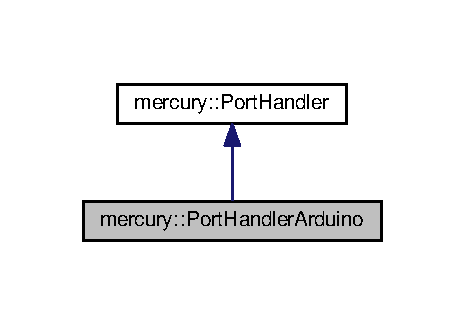
\includegraphics[width=223pt]{classmercury_1_1_port_handler_arduino__inherit__graph}
\end{center}
\end{figure}


Collaboration diagram for mercury\+:\+:Port\+Handler\+Arduino\+:\nopagebreak
\begin{figure}[H]
\begin{center}
\leavevmode
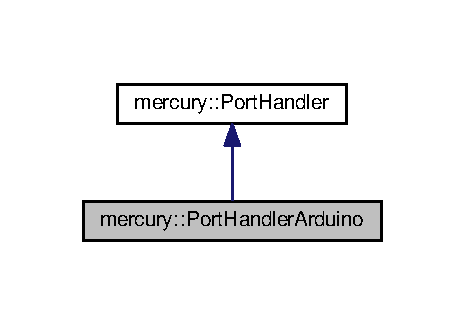
\includegraphics[width=223pt]{classmercury_1_1_port_handler_arduino__coll__graph}
\end{center}
\end{figure}
\subsection*{Public Member Functions}
\begin{DoxyCompactItemize}
\item 
\hyperlink{classmercury_1_1_port_handler_arduino_a54481f6e17666c6e04f721149f8e70f8}{Port\+Handler\+Arduino} (const char $\ast$port\+\_\+name)\hypertarget{classmercury_1_1_port_handler_arduino_a54481f6e17666c6e04f721149f8e70f8}{}\label{classmercury_1_1_port_handler_arduino_a54481f6e17666c6e04f721149f8e70f8}

\begin{DoxyCompactList}\small\item\em The function that initializes instance of \hyperlink{classmercury_1_1_port_handler}{Port\+Handler} and gets port\+\_\+name  The function initializes instance of \hyperlink{classmercury_1_1_port_handler}{Port\+Handler} and gets port\+\_\+name. \end{DoxyCompactList}\item 
virtual \hyperlink{classmercury_1_1_port_handler_arduino_a09890b269b6a041ef96289fbf7f0e9fd}{$\sim$\+Port\+Handler\+Arduino} ()\hypertarget{classmercury_1_1_port_handler_arduino_a09890b269b6a041ef96289fbf7f0e9fd}{}\label{classmercury_1_1_port_handler_arduino_a09890b269b6a041ef96289fbf7f0e9fd}

\begin{DoxyCompactList}\small\item\em The function that closes the port  The function calls \hyperlink{classmercury_1_1_port_handler_arduino_a56c560c6ea70258f04ecf1c529b06e70}{Port\+Handler\+Arduino\+::close\+Port()} to close the port. \end{DoxyCompactList}\item 
bool \hyperlink{classmercury_1_1_port_handler_arduino_a998afa0864dda7b2891238a37ebd06b7}{open\+Port} ()
\begin{DoxyCompactList}\small\item\em The function that opens the port  The function calls \hyperlink{classmercury_1_1_port_handler_arduino_a6cf1955442f7c93cbd83adde3cebc17e}{Port\+Handler\+Arduino\+::set\+Baud\+Rate()} to open the port. \end{DoxyCompactList}\item 
void \hyperlink{classmercury_1_1_port_handler_arduino_a56c560c6ea70258f04ecf1c529b06e70}{close\+Port} ()\hypertarget{classmercury_1_1_port_handler_arduino_a56c560c6ea70258f04ecf1c529b06e70}{}\label{classmercury_1_1_port_handler_arduino_a56c560c6ea70258f04ecf1c529b06e70}

\begin{DoxyCompactList}\small\item\em The function that closes the port  The function closes the port. \end{DoxyCompactList}\item 
void \hyperlink{classmercury_1_1_port_handler_arduino_ae5a4b9f34e92c1b9862bfa38de457bc6}{clear\+Port} ()\hypertarget{classmercury_1_1_port_handler_arduino_ae5a4b9f34e92c1b9862bfa38de457bc6}{}\label{classmercury_1_1_port_handler_arduino_ae5a4b9f34e92c1b9862bfa38de457bc6}

\begin{DoxyCompactList}\small\item\em The function that clears the port  The function clears the port. \end{DoxyCompactList}\item 
void \hyperlink{classmercury_1_1_port_handler_arduino_ae868b2b94cd47884bff283aab3418f12}{set\+Port\+Name} (const char $\ast$port\+\_\+name)
\begin{DoxyCompactList}\small\item\em The function that sets port name into the port handler  The function sets port name into the port handler. \end{DoxyCompactList}\item 
char $\ast$ \hyperlink{classmercury_1_1_port_handler_arduino_a356c7c38cbdf5ceb75b3192c8910b076}{get\+Port\+Name} ()
\begin{DoxyCompactList}\small\item\em The function that returns port name set into the port handler  The function returns current port name set into the port handler. \end{DoxyCompactList}\item 
bool \hyperlink{classmercury_1_1_port_handler_arduino_a6cf1955442f7c93cbd83adde3cebc17e}{set\+Baud\+Rate} (const int baudrate)
\begin{DoxyCompactList}\small\item\em The function that sets baudrate into the port handler  The function sets baudrate into the port handler. \end{DoxyCompactList}\item 
int \hyperlink{classmercury_1_1_port_handler_arduino_a26dc1b14d340b49cb43480f5fb7f177f}{get\+Baud\+Rate} ()
\begin{DoxyCompactList}\small\item\em The function that returns current baudrate set into the port handler  The function returns current baudrate set into the port handler. \end{DoxyCompactList}\item 
int \hyperlink{classmercury_1_1_port_handler_arduino_a538c84a114d4c60e3a75cca75b2998a8}{get\+Bytes\+Available} ()
\begin{DoxyCompactList}\small\item\em The function that checks how much bytes are able to be read from the port buffer  The function checks how much bytes are able to be read from the port buffer  and returns the number. \end{DoxyCompactList}\item 
int \hyperlink{classmercury_1_1_port_handler_arduino_a4fcf4a5a3981715258637198a00b4d4c}{read\+Port} (uint8\+\_\+t $\ast$packet, int length)
\begin{DoxyCompactList}\small\item\em The function that reads bytes from the port buffer  The function gets bytes from the port buffer,  and returns a number of bytes read. \end{DoxyCompactList}\item 
int \hyperlink{classmercury_1_1_port_handler_arduino_a92cd2b66a8ed120e21bc78e3b83ce15d}{write\+Port} (uint8\+\_\+t $\ast$packet, int length)
\begin{DoxyCompactList}\small\item\em The function that writes bytes on the port buffer  The function writes bytes on the port buffer,  and returns a number of bytes which are successfully written. \end{DoxyCompactList}\item 
void \hyperlink{classmercury_1_1_port_handler_arduino_ad9f8b2e9d24b8117a9ffcd99f73c78ef}{set\+Packet\+Timeout} (uint16\+\_\+t packet\+\_\+length)
\begin{DoxyCompactList}\small\item\em The function that sets and starts stopwatch for watching packet timeout  The function sets the stopwatch by getting current time and the time of packet timeout with packet\+\_\+length. \end{DoxyCompactList}\item 
void \hyperlink{classmercury_1_1_port_handler_arduino_a8d47dc2fc47a025d9285f1739356bfea}{set\+Packet\+Timeout} (double msec)
\begin{DoxyCompactList}\small\item\em The function that sets and starts stopwatch for watching packet timeout  The function sets the stopwatch by getting current time and the time of packet timeout with msec. \end{DoxyCompactList}\item 
bool \hyperlink{classmercury_1_1_port_handler_arduino_aa20b1c76747b9da4631700d1ad4f9584}{is\+Packet\+Timeout} ()\hypertarget{classmercury_1_1_port_handler_arduino_aa20b1c76747b9da4631700d1ad4f9584}{}\label{classmercury_1_1_port_handler_arduino_aa20b1c76747b9da4631700d1ad4f9584}

\begin{DoxyCompactList}\small\item\em The function that checks whether packet timeout is occurred  The function checks whether current time is passed by the time of packet timeout from the time set by \hyperlink{classmercury_1_1_port_handler_arduino_ad9f8b2e9d24b8117a9ffcd99f73c78ef}{Port\+Handler\+Arduino\+::set\+Packet\+Timeout()}. \end{DoxyCompactList}\end{DoxyCompactItemize}
\subsection*{Additional Inherited Members}


\subsection{Detailed Description}
The class for control port in Arduino. 

\subsection{Member Function Documentation}
\index{mercury\+::\+Port\+Handler\+Arduino@{mercury\+::\+Port\+Handler\+Arduino}!get\+Baud\+Rate@{get\+Baud\+Rate}}
\index{get\+Baud\+Rate@{get\+Baud\+Rate}!mercury\+::\+Port\+Handler\+Arduino@{mercury\+::\+Port\+Handler\+Arduino}}
\subsubsection[{\texorpdfstring{get\+Baud\+Rate()}{getBaudRate()}}]{\setlength{\rightskip}{0pt plus 5cm}int mercury\+::\+Port\+Handler\+Arduino\+::get\+Baud\+Rate (
\begin{DoxyParamCaption}
{}
\end{DoxyParamCaption}
)\hspace{0.3cm}{\ttfamily [virtual]}}\hypertarget{classmercury_1_1_port_handler_arduino_a26dc1b14d340b49cb43480f5fb7f177f}{}\label{classmercury_1_1_port_handler_arduino_a26dc1b14d340b49cb43480f5fb7f177f}


The function that returns current baudrate set into the port handler  The function returns current baudrate set into the port handler. 

\begin{DoxyReturn}{Returns}
Baudrate 
\end{DoxyReturn}


Implements \hyperlink{classmercury_1_1_port_handler_a686c731714c095ac194847cd585643ea}{mercury\+::\+Port\+Handler}.

\index{mercury\+::\+Port\+Handler\+Arduino@{mercury\+::\+Port\+Handler\+Arduino}!get\+Bytes\+Available@{get\+Bytes\+Available}}
\index{get\+Bytes\+Available@{get\+Bytes\+Available}!mercury\+::\+Port\+Handler\+Arduino@{mercury\+::\+Port\+Handler\+Arduino}}
\subsubsection[{\texorpdfstring{get\+Bytes\+Available()}{getBytesAvailable()}}]{\setlength{\rightskip}{0pt plus 5cm}int mercury\+::\+Port\+Handler\+Arduino\+::get\+Bytes\+Available (
\begin{DoxyParamCaption}
{}
\end{DoxyParamCaption}
)\hspace{0.3cm}{\ttfamily [virtual]}}\hypertarget{classmercury_1_1_port_handler_arduino_a538c84a114d4c60e3a75cca75b2998a8}{}\label{classmercury_1_1_port_handler_arduino_a538c84a114d4c60e3a75cca75b2998a8}


The function that checks how much bytes are able to be read from the port buffer  The function checks how much bytes are able to be read from the port buffer  and returns the number. 

\begin{DoxyReturn}{Returns}
Length of read-\/able bytes in the port buffer 
\end{DoxyReturn}


Implements \hyperlink{classmercury_1_1_port_handler_a2c0a25741b4b8d15e19e619ed7b5a148}{mercury\+::\+Port\+Handler}.

\index{mercury\+::\+Port\+Handler\+Arduino@{mercury\+::\+Port\+Handler\+Arduino}!get\+Port\+Name@{get\+Port\+Name}}
\index{get\+Port\+Name@{get\+Port\+Name}!mercury\+::\+Port\+Handler\+Arduino@{mercury\+::\+Port\+Handler\+Arduino}}
\subsubsection[{\texorpdfstring{get\+Port\+Name()}{getPortName()}}]{\setlength{\rightskip}{0pt plus 5cm}char$\ast$ mercury\+::\+Port\+Handler\+Arduino\+::get\+Port\+Name (
\begin{DoxyParamCaption}
{}
\end{DoxyParamCaption}
)\hspace{0.3cm}{\ttfamily [virtual]}}\hypertarget{classmercury_1_1_port_handler_arduino_a356c7c38cbdf5ceb75b3192c8910b076}{}\label{classmercury_1_1_port_handler_arduino_a356c7c38cbdf5ceb75b3192c8910b076}


The function that returns port name set into the port handler  The function returns current port name set into the port handler. 

\begin{DoxyReturn}{Returns}
Port name 
\end{DoxyReturn}


Implements \hyperlink{classmercury_1_1_port_handler_ab6e0df491f6a6b4f927401e60c0c9c5c}{mercury\+::\+Port\+Handler}.

\index{mercury\+::\+Port\+Handler\+Arduino@{mercury\+::\+Port\+Handler\+Arduino}!open\+Port@{open\+Port}}
\index{open\+Port@{open\+Port}!mercury\+::\+Port\+Handler\+Arduino@{mercury\+::\+Port\+Handler\+Arduino}}
\subsubsection[{\texorpdfstring{open\+Port()}{openPort()}}]{\setlength{\rightskip}{0pt plus 5cm}bool mercury\+::\+Port\+Handler\+Arduino\+::open\+Port (
\begin{DoxyParamCaption}
{}
\end{DoxyParamCaption}
)\hspace{0.3cm}{\ttfamily [virtual]}}\hypertarget{classmercury_1_1_port_handler_arduino_a998afa0864dda7b2891238a37ebd06b7}{}\label{classmercury_1_1_port_handler_arduino_a998afa0864dda7b2891238a37ebd06b7}


The function that opens the port  The function calls \hyperlink{classmercury_1_1_port_handler_arduino_a6cf1955442f7c93cbd83adde3cebc17e}{Port\+Handler\+Arduino\+::set\+Baud\+Rate()} to open the port. 

\begin{DoxyReturn}{Returns}
communication results which come from \hyperlink{classmercury_1_1_port_handler_arduino_a6cf1955442f7c93cbd83adde3cebc17e}{Port\+Handler\+Arduino\+::set\+Baud\+Rate()} 
\end{DoxyReturn}


Implements \hyperlink{classmercury_1_1_port_handler_a5f65f9a73969cc170582da2d0e11f510}{mercury\+::\+Port\+Handler}.

\index{mercury\+::\+Port\+Handler\+Arduino@{mercury\+::\+Port\+Handler\+Arduino}!read\+Port@{read\+Port}}
\index{read\+Port@{read\+Port}!mercury\+::\+Port\+Handler\+Arduino@{mercury\+::\+Port\+Handler\+Arduino}}
\subsubsection[{\texorpdfstring{read\+Port(uint8\+\_\+t $\ast$packet, int length)}{readPort(uint8_t *packet, int length)}}]{\setlength{\rightskip}{0pt plus 5cm}int mercury\+::\+Port\+Handler\+Arduino\+::read\+Port (
\begin{DoxyParamCaption}
\item[{uint8\+\_\+t $\ast$}]{packet, }
\item[{int}]{length}
\end{DoxyParamCaption}
)\hspace{0.3cm}{\ttfamily [virtual]}}\hypertarget{classmercury_1_1_port_handler_arduino_a4fcf4a5a3981715258637198a00b4d4c}{}\label{classmercury_1_1_port_handler_arduino_a4fcf4a5a3981715258637198a00b4d4c}


The function that reads bytes from the port buffer  The function gets bytes from the port buffer,  and returns a number of bytes read. 


\begin{DoxyParams}{Parameters}
{\em packet} & Buffer for the packet received \\
\hline
{\em length} & Length of the buffer for read \\
\hline
\end{DoxyParams}
\begin{DoxyReturn}{Returns}
-\/1 

when error was occurred 

or Length of bytes read 
\end{DoxyReturn}


Implements \hyperlink{classmercury_1_1_port_handler_afa6f52d7b95c5ffd8f0c92477d517c79}{mercury\+::\+Port\+Handler}.

\index{mercury\+::\+Port\+Handler\+Arduino@{mercury\+::\+Port\+Handler\+Arduino}!set\+Baud\+Rate@{set\+Baud\+Rate}}
\index{set\+Baud\+Rate@{set\+Baud\+Rate}!mercury\+::\+Port\+Handler\+Arduino@{mercury\+::\+Port\+Handler\+Arduino}}
\subsubsection[{\texorpdfstring{set\+Baud\+Rate(const int baudrate)}{setBaudRate(const int baudrate)}}]{\setlength{\rightskip}{0pt plus 5cm}bool mercury\+::\+Port\+Handler\+Arduino\+::set\+Baud\+Rate (
\begin{DoxyParamCaption}
\item[{const int}]{baudrate}
\end{DoxyParamCaption}
)\hspace{0.3cm}{\ttfamily [virtual]}}\hypertarget{classmercury_1_1_port_handler_arduino_a6cf1955442f7c93cbd83adde3cebc17e}{}\label{classmercury_1_1_port_handler_arduino_a6cf1955442f7c93cbd83adde3cebc17e}


The function that sets baudrate into the port handler  The function sets baudrate into the port handler. 


\begin{DoxyParams}{Parameters}
{\em baudrate} & Baudrate \\
\hline
\end{DoxyParams}
\begin{DoxyReturn}{Returns}
false 

when error was occurred during port opening 

or true 
\end{DoxyReturn}


Implements \hyperlink{classmercury_1_1_port_handler_a663168c32580a532ccb328544565f06d}{mercury\+::\+Port\+Handler}.

\index{mercury\+::\+Port\+Handler\+Arduino@{mercury\+::\+Port\+Handler\+Arduino}!set\+Packet\+Timeout@{set\+Packet\+Timeout}}
\index{set\+Packet\+Timeout@{set\+Packet\+Timeout}!mercury\+::\+Port\+Handler\+Arduino@{mercury\+::\+Port\+Handler\+Arduino}}
\subsubsection[{\texorpdfstring{set\+Packet\+Timeout(uint16\+\_\+t packet\+\_\+length)}{setPacketTimeout(uint16_t packet_length)}}]{\setlength{\rightskip}{0pt plus 5cm}void mercury\+::\+Port\+Handler\+Arduino\+::set\+Packet\+Timeout (
\begin{DoxyParamCaption}
\item[{uint16\+\_\+t}]{packet\+\_\+length}
\end{DoxyParamCaption}
)\hspace{0.3cm}{\ttfamily [virtual]}}\hypertarget{classmercury_1_1_port_handler_arduino_ad9f8b2e9d24b8117a9ffcd99f73c78ef}{}\label{classmercury_1_1_port_handler_arduino_ad9f8b2e9d24b8117a9ffcd99f73c78ef}


The function that sets and starts stopwatch for watching packet timeout  The function sets the stopwatch by getting current time and the time of packet timeout with packet\+\_\+length. 


\begin{DoxyParams}{Parameters}
{\em packet\+\_\+length} & Length of the packet expected to be received \\
\hline
\end{DoxyParams}


Implements \hyperlink{classmercury_1_1_port_handler_ae79ec2448529ffc2f1788da26142d164}{mercury\+::\+Port\+Handler}.

\index{mercury\+::\+Port\+Handler\+Arduino@{mercury\+::\+Port\+Handler\+Arduino}!set\+Packet\+Timeout@{set\+Packet\+Timeout}}
\index{set\+Packet\+Timeout@{set\+Packet\+Timeout}!mercury\+::\+Port\+Handler\+Arduino@{mercury\+::\+Port\+Handler\+Arduino}}
\subsubsection[{\texorpdfstring{set\+Packet\+Timeout(double msec)}{setPacketTimeout(double msec)}}]{\setlength{\rightskip}{0pt plus 5cm}void mercury\+::\+Port\+Handler\+Arduino\+::set\+Packet\+Timeout (
\begin{DoxyParamCaption}
\item[{double}]{msec}
\end{DoxyParamCaption}
)\hspace{0.3cm}{\ttfamily [virtual]}}\hypertarget{classmercury_1_1_port_handler_arduino_a8d47dc2fc47a025d9285f1739356bfea}{}\label{classmercury_1_1_port_handler_arduino_a8d47dc2fc47a025d9285f1739356bfea}


The function that sets and starts stopwatch for watching packet timeout  The function sets the stopwatch by getting current time and the time of packet timeout with msec. 


\begin{DoxyParams}{Parameters}
{\em packet\+\_\+length} & Length of the packet expected to be received \\
\hline
\end{DoxyParams}


Implements \hyperlink{classmercury_1_1_port_handler_ae61a4953ef52be49401af210acf820a4}{mercury\+::\+Port\+Handler}.

\index{mercury\+::\+Port\+Handler\+Arduino@{mercury\+::\+Port\+Handler\+Arduino}!set\+Port\+Name@{set\+Port\+Name}}
\index{set\+Port\+Name@{set\+Port\+Name}!mercury\+::\+Port\+Handler\+Arduino@{mercury\+::\+Port\+Handler\+Arduino}}
\subsubsection[{\texorpdfstring{set\+Port\+Name(const char $\ast$port\+\_\+name)}{setPortName(const char *port_name)}}]{\setlength{\rightskip}{0pt plus 5cm}void mercury\+::\+Port\+Handler\+Arduino\+::set\+Port\+Name (
\begin{DoxyParamCaption}
\item[{const char $\ast$}]{port\+\_\+name}
\end{DoxyParamCaption}
)\hspace{0.3cm}{\ttfamily [virtual]}}\hypertarget{classmercury_1_1_port_handler_arduino_ae868b2b94cd47884bff283aab3418f12}{}\label{classmercury_1_1_port_handler_arduino_ae868b2b94cd47884bff283aab3418f12}


The function that sets port name into the port handler  The function sets port name into the port handler. 


\begin{DoxyParams}{Parameters}
{\em port\+\_\+name} & Port name \\
\hline
\end{DoxyParams}


Implements \hyperlink{classmercury_1_1_port_handler_adb0bff39482904066c1bdd7713441e9e}{mercury\+::\+Port\+Handler}.

\index{mercury\+::\+Port\+Handler\+Arduino@{mercury\+::\+Port\+Handler\+Arduino}!write\+Port@{write\+Port}}
\index{write\+Port@{write\+Port}!mercury\+::\+Port\+Handler\+Arduino@{mercury\+::\+Port\+Handler\+Arduino}}
\subsubsection[{\texorpdfstring{write\+Port(uint8\+\_\+t $\ast$packet, int length)}{writePort(uint8_t *packet, int length)}}]{\setlength{\rightskip}{0pt plus 5cm}int mercury\+::\+Port\+Handler\+Arduino\+::write\+Port (
\begin{DoxyParamCaption}
\item[{uint8\+\_\+t $\ast$}]{packet, }
\item[{int}]{length}
\end{DoxyParamCaption}
)\hspace{0.3cm}{\ttfamily [virtual]}}\hypertarget{classmercury_1_1_port_handler_arduino_a92cd2b66a8ed120e21bc78e3b83ce15d}{}\label{classmercury_1_1_port_handler_arduino_a92cd2b66a8ed120e21bc78e3b83ce15d}


The function that writes bytes on the port buffer  The function writes bytes on the port buffer,  and returns a number of bytes which are successfully written. 


\begin{DoxyParams}{Parameters}
{\em packet} & Buffer which would be written on the port buffer \\
\hline
{\em length} & Length of the buffer for write \\
\hline
\end{DoxyParams}
\begin{DoxyReturn}{Returns}
-\/1 

when error was occurred 

or Length of bytes written 
\end{DoxyReturn}


Implements \hyperlink{classmercury_1_1_port_handler_ad26c3a106d6b668b6fae3d2f0afeab9e}{mercury\+::\+Port\+Handler}.



The documentation for this class was generated from the following file\+:\begin{DoxyCompactItemize}
\item 
/home/wigir/dev/software/projects/\+Mercury\+S\+D\+K/c++/include/mercury\+\_\+sdk/port\+\_\+handler\+\_\+arduino.\+h\end{DoxyCompactItemize}

\hypertarget{classmercury_1_1_port_handler_linux}{}\section{mercury\+:\+:Port\+Handler\+Linux Class Reference}
\label{classmercury_1_1_port_handler_linux}\index{mercury\+::\+Port\+Handler\+Linux@{mercury\+::\+Port\+Handler\+Linux}}


The class for control port in Linux.  




{\ttfamily \#include $<$port\+\_\+handler\+\_\+linux.\+h$>$}



Inheritance diagram for mercury\+:\+:Port\+Handler\+Linux\+:\nopagebreak
\begin{figure}[H]
\begin{center}
\leavevmode
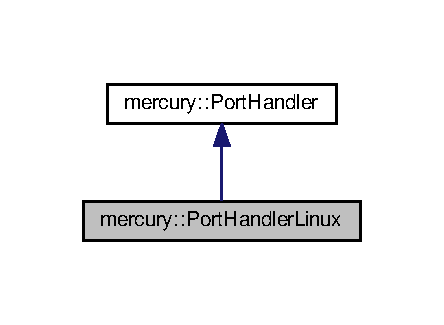
\includegraphics[width=213pt]{classmercury_1_1_port_handler_linux__inherit__graph}
\end{center}
\end{figure}


Collaboration diagram for mercury\+:\+:Port\+Handler\+Linux\+:\nopagebreak
\begin{figure}[H]
\begin{center}
\leavevmode
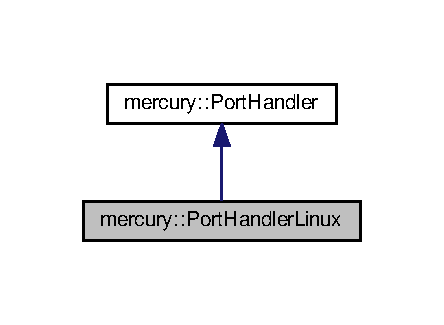
\includegraphics[width=213pt]{classmercury_1_1_port_handler_linux__coll__graph}
\end{center}
\end{figure}
\subsection*{Public Member Functions}
\begin{DoxyCompactItemize}
\item 
\hyperlink{classmercury_1_1_port_handler_linux_ac47ba79fd979eaaf39c89f6cfb5aada6}{Port\+Handler\+Linux} (const char $\ast$port\+\_\+name)\hypertarget{classmercury_1_1_port_handler_linux_ac47ba79fd979eaaf39c89f6cfb5aada6}{}\label{classmercury_1_1_port_handler_linux_ac47ba79fd979eaaf39c89f6cfb5aada6}

\begin{DoxyCompactList}\small\item\em The function that initializes instance of \hyperlink{classmercury_1_1_port_handler}{Port\+Handler} and gets port\+\_\+name  The function initializes instance of \hyperlink{classmercury_1_1_port_handler}{Port\+Handler} and gets port\+\_\+name. \end{DoxyCompactList}\item 
virtual \hyperlink{classmercury_1_1_port_handler_linux_ad950209aa592c09365d824ae1f21b28d}{$\sim$\+Port\+Handler\+Linux} ()\hypertarget{classmercury_1_1_port_handler_linux_ad950209aa592c09365d824ae1f21b28d}{}\label{classmercury_1_1_port_handler_linux_ad950209aa592c09365d824ae1f21b28d}

\begin{DoxyCompactList}\small\item\em The function that closes the port  The function calls \hyperlink{classmercury_1_1_port_handler_linux_ab224a54b1137daa5b542eb6ad38491da}{Port\+Handler\+Linux\+::close\+Port()} to close the port. \end{DoxyCompactList}\item 
bool \hyperlink{classmercury_1_1_port_handler_linux_aa28ad8fa7617a396f5fd347e716af964}{open\+Port} ()
\begin{DoxyCompactList}\small\item\em The function that opens the port  The function calls \hyperlink{classmercury_1_1_port_handler_linux_a31c5d6a569cec58d20f9041f100a637c}{Port\+Handler\+Linux\+::set\+Baud\+Rate()} to open the port. \end{DoxyCompactList}\item 
void \hyperlink{classmercury_1_1_port_handler_linux_ab224a54b1137daa5b542eb6ad38491da}{close\+Port} ()\hypertarget{classmercury_1_1_port_handler_linux_ab224a54b1137daa5b542eb6ad38491da}{}\label{classmercury_1_1_port_handler_linux_ab224a54b1137daa5b542eb6ad38491da}

\begin{DoxyCompactList}\small\item\em The function that closes the port  The function closes the port. \end{DoxyCompactList}\item 
void \hyperlink{classmercury_1_1_port_handler_linux_a13b3b62f0ba3b441e20c91ca0ccbc311}{clear\+Port} ()\hypertarget{classmercury_1_1_port_handler_linux_a13b3b62f0ba3b441e20c91ca0ccbc311}{}\label{classmercury_1_1_port_handler_linux_a13b3b62f0ba3b441e20c91ca0ccbc311}

\begin{DoxyCompactList}\small\item\em The function that clears the port  The function clears the port. \end{DoxyCompactList}\item 
void \hyperlink{classmercury_1_1_port_handler_linux_a91530ad73312a7c3a8e52c219d2b04f5}{set\+Port\+Name} (const char $\ast$port\+\_\+name)
\begin{DoxyCompactList}\small\item\em The function that sets port name into the port handler  The function sets port name into the port handler. \end{DoxyCompactList}\item 
char $\ast$ \hyperlink{classmercury_1_1_port_handler_linux_a2bfe34d53f78e0266de06e9cd4e58193}{get\+Port\+Name} ()
\begin{DoxyCompactList}\small\item\em The function that returns port name set into the port handler  The function returns current port name set into the port handler. \end{DoxyCompactList}\item 
bool \hyperlink{classmercury_1_1_port_handler_linux_a31c5d6a569cec58d20f9041f100a637c}{set\+Baud\+Rate} (const int baudrate)
\begin{DoxyCompactList}\small\item\em The function that sets baudrate into the port handler  The function sets baudrate into the port handler. \end{DoxyCompactList}\item 
int \hyperlink{classmercury_1_1_port_handler_linux_aa2deb65e4f97877e9d1b4b84c7b4d433}{get\+Baud\+Rate} ()
\begin{DoxyCompactList}\small\item\em The function that returns current baudrate set into the port handler  The function returns current baudrate set into the port handler. \end{DoxyCompactList}\item 
int \hyperlink{classmercury_1_1_port_handler_linux_a632cebf3de5cd02825ba3493f47e28fa}{get\+Bytes\+Available} ()
\begin{DoxyCompactList}\small\item\em The function that checks how much bytes are able to be read from the port buffer  The function checks how much bytes are able to be read from the port buffer  and returns the number. \end{DoxyCompactList}\item 
int \hyperlink{classmercury_1_1_port_handler_linux_ac4667b4e9350fffa2163ee547cce1b88}{read\+Port} (uint8\+\_\+t $\ast$packet, int length)
\begin{DoxyCompactList}\small\item\em The function that reads bytes from the port buffer  The function gets bytes from the port buffer,  and returns a number of bytes read. \end{DoxyCompactList}\item 
int \hyperlink{classmercury_1_1_port_handler_linux_af9688d8e104e1a083958347091f234d7}{write\+Port} (uint8\+\_\+t $\ast$packet, int length)
\begin{DoxyCompactList}\small\item\em The function that writes bytes on the port buffer  The function writes bytes on the port buffer,  and returns a number of bytes which are successfully written. \end{DoxyCompactList}\item 
void \hyperlink{classmercury_1_1_port_handler_linux_a3b3e75d2f295fb4453b2f5a531110c7e}{set\+Packet\+Timeout} (uint16\+\_\+t packet\+\_\+length)
\begin{DoxyCompactList}\small\item\em The function that sets and starts stopwatch for watching packet timeout  The function sets the stopwatch by getting current time and the time of packet timeout with packet\+\_\+length. \end{DoxyCompactList}\item 
void \hyperlink{classmercury_1_1_port_handler_linux_af998c701488acf2581dbc5f5a36a3588}{set\+Packet\+Timeout} (double msec)
\begin{DoxyCompactList}\small\item\em The function that sets and starts stopwatch for watching packet timeout  The function sets the stopwatch by getting current time and the time of packet timeout with msec. \end{DoxyCompactList}\item 
bool \hyperlink{classmercury_1_1_port_handler_linux_a389d65f59f704306acda863748638918}{is\+Packet\+Timeout} ()\hypertarget{classmercury_1_1_port_handler_linux_a389d65f59f704306acda863748638918}{}\label{classmercury_1_1_port_handler_linux_a389d65f59f704306acda863748638918}

\begin{DoxyCompactList}\small\item\em The function that checks whether packet timeout is occurred  The function checks whether current time is passed by the time of packet timeout from the time set by \hyperlink{classmercury_1_1_port_handler_linux_a3b3e75d2f295fb4453b2f5a531110c7e}{Port\+Handler\+Linux\+::set\+Packet\+Timeout()}. \end{DoxyCompactList}\end{DoxyCompactItemize}
\subsection*{Additional Inherited Members}


\subsection{Detailed Description}
The class for control port in Linux. 

\subsection{Member Function Documentation}
\index{mercury\+::\+Port\+Handler\+Linux@{mercury\+::\+Port\+Handler\+Linux}!get\+Baud\+Rate@{get\+Baud\+Rate}}
\index{get\+Baud\+Rate@{get\+Baud\+Rate}!mercury\+::\+Port\+Handler\+Linux@{mercury\+::\+Port\+Handler\+Linux}}
\subsubsection[{\texorpdfstring{get\+Baud\+Rate()}{getBaudRate()}}]{\setlength{\rightskip}{0pt plus 5cm}int mercury\+::\+Port\+Handler\+Linux\+::get\+Baud\+Rate (
\begin{DoxyParamCaption}
{}
\end{DoxyParamCaption}
)\hspace{0.3cm}{\ttfamily [virtual]}}\hypertarget{classmercury_1_1_port_handler_linux_aa2deb65e4f97877e9d1b4b84c7b4d433}{}\label{classmercury_1_1_port_handler_linux_aa2deb65e4f97877e9d1b4b84c7b4d433}


The function that returns current baudrate set into the port handler  The function returns current baudrate set into the port handler. 

\begin{DoxyReturn}{Returns}
Baudrate 
\end{DoxyReturn}


Implements \hyperlink{classmercury_1_1_port_handler_a686c731714c095ac194847cd585643ea}{mercury\+::\+Port\+Handler}.

\index{mercury\+::\+Port\+Handler\+Linux@{mercury\+::\+Port\+Handler\+Linux}!get\+Bytes\+Available@{get\+Bytes\+Available}}
\index{get\+Bytes\+Available@{get\+Bytes\+Available}!mercury\+::\+Port\+Handler\+Linux@{mercury\+::\+Port\+Handler\+Linux}}
\subsubsection[{\texorpdfstring{get\+Bytes\+Available()}{getBytesAvailable()}}]{\setlength{\rightskip}{0pt plus 5cm}int mercury\+::\+Port\+Handler\+Linux\+::get\+Bytes\+Available (
\begin{DoxyParamCaption}
{}
\end{DoxyParamCaption}
)\hspace{0.3cm}{\ttfamily [virtual]}}\hypertarget{classmercury_1_1_port_handler_linux_a632cebf3de5cd02825ba3493f47e28fa}{}\label{classmercury_1_1_port_handler_linux_a632cebf3de5cd02825ba3493f47e28fa}


The function that checks how much bytes are able to be read from the port buffer  The function checks how much bytes are able to be read from the port buffer  and returns the number. 

\begin{DoxyReturn}{Returns}
Length of read-\/able bytes in the port buffer 
\end{DoxyReturn}


Implements \hyperlink{classmercury_1_1_port_handler_a2c0a25741b4b8d15e19e619ed7b5a148}{mercury\+::\+Port\+Handler}.

\index{mercury\+::\+Port\+Handler\+Linux@{mercury\+::\+Port\+Handler\+Linux}!get\+Port\+Name@{get\+Port\+Name}}
\index{get\+Port\+Name@{get\+Port\+Name}!mercury\+::\+Port\+Handler\+Linux@{mercury\+::\+Port\+Handler\+Linux}}
\subsubsection[{\texorpdfstring{get\+Port\+Name()}{getPortName()}}]{\setlength{\rightskip}{0pt plus 5cm}char$\ast$ mercury\+::\+Port\+Handler\+Linux\+::get\+Port\+Name (
\begin{DoxyParamCaption}
{}
\end{DoxyParamCaption}
)\hspace{0.3cm}{\ttfamily [virtual]}}\hypertarget{classmercury_1_1_port_handler_linux_a2bfe34d53f78e0266de06e9cd4e58193}{}\label{classmercury_1_1_port_handler_linux_a2bfe34d53f78e0266de06e9cd4e58193}


The function that returns port name set into the port handler  The function returns current port name set into the port handler. 

\begin{DoxyReturn}{Returns}
Port name 
\end{DoxyReturn}


Implements \hyperlink{classmercury_1_1_port_handler_ab6e0df491f6a6b4f927401e60c0c9c5c}{mercury\+::\+Port\+Handler}.

\index{mercury\+::\+Port\+Handler\+Linux@{mercury\+::\+Port\+Handler\+Linux}!open\+Port@{open\+Port}}
\index{open\+Port@{open\+Port}!mercury\+::\+Port\+Handler\+Linux@{mercury\+::\+Port\+Handler\+Linux}}
\subsubsection[{\texorpdfstring{open\+Port()}{openPort()}}]{\setlength{\rightskip}{0pt plus 5cm}bool mercury\+::\+Port\+Handler\+Linux\+::open\+Port (
\begin{DoxyParamCaption}
{}
\end{DoxyParamCaption}
)\hspace{0.3cm}{\ttfamily [virtual]}}\hypertarget{classmercury_1_1_port_handler_linux_aa28ad8fa7617a396f5fd347e716af964}{}\label{classmercury_1_1_port_handler_linux_aa28ad8fa7617a396f5fd347e716af964}


The function that opens the port  The function calls \hyperlink{classmercury_1_1_port_handler_linux_a31c5d6a569cec58d20f9041f100a637c}{Port\+Handler\+Linux\+::set\+Baud\+Rate()} to open the port. 

\begin{DoxyReturn}{Returns}
communication results which come from \hyperlink{classmercury_1_1_port_handler_linux_a31c5d6a569cec58d20f9041f100a637c}{Port\+Handler\+Linux\+::set\+Baud\+Rate()} 
\end{DoxyReturn}


Implements \hyperlink{classmercury_1_1_port_handler_a5f65f9a73969cc170582da2d0e11f510}{mercury\+::\+Port\+Handler}.

\index{mercury\+::\+Port\+Handler\+Linux@{mercury\+::\+Port\+Handler\+Linux}!read\+Port@{read\+Port}}
\index{read\+Port@{read\+Port}!mercury\+::\+Port\+Handler\+Linux@{mercury\+::\+Port\+Handler\+Linux}}
\subsubsection[{\texorpdfstring{read\+Port(uint8\+\_\+t $\ast$packet, int length)}{readPort(uint8_t *packet, int length)}}]{\setlength{\rightskip}{0pt plus 5cm}int mercury\+::\+Port\+Handler\+Linux\+::read\+Port (
\begin{DoxyParamCaption}
\item[{uint8\+\_\+t $\ast$}]{packet, }
\item[{int}]{length}
\end{DoxyParamCaption}
)\hspace{0.3cm}{\ttfamily [virtual]}}\hypertarget{classmercury_1_1_port_handler_linux_ac4667b4e9350fffa2163ee547cce1b88}{}\label{classmercury_1_1_port_handler_linux_ac4667b4e9350fffa2163ee547cce1b88}


The function that reads bytes from the port buffer  The function gets bytes from the port buffer,  and returns a number of bytes read. 


\begin{DoxyParams}{Parameters}
{\em packet} & Buffer for the packet received \\
\hline
{\em length} & Length of the buffer for read \\
\hline
\end{DoxyParams}
\begin{DoxyReturn}{Returns}
-\/1 

when error was occurred 

or Length of bytes read 
\end{DoxyReturn}


Implements \hyperlink{classmercury_1_1_port_handler_afa6f52d7b95c5ffd8f0c92477d517c79}{mercury\+::\+Port\+Handler}.

\index{mercury\+::\+Port\+Handler\+Linux@{mercury\+::\+Port\+Handler\+Linux}!set\+Baud\+Rate@{set\+Baud\+Rate}}
\index{set\+Baud\+Rate@{set\+Baud\+Rate}!mercury\+::\+Port\+Handler\+Linux@{mercury\+::\+Port\+Handler\+Linux}}
\subsubsection[{\texorpdfstring{set\+Baud\+Rate(const int baudrate)}{setBaudRate(const int baudrate)}}]{\setlength{\rightskip}{0pt plus 5cm}bool mercury\+::\+Port\+Handler\+Linux\+::set\+Baud\+Rate (
\begin{DoxyParamCaption}
\item[{const int}]{baudrate}
\end{DoxyParamCaption}
)\hspace{0.3cm}{\ttfamily [virtual]}}\hypertarget{classmercury_1_1_port_handler_linux_a31c5d6a569cec58d20f9041f100a637c}{}\label{classmercury_1_1_port_handler_linux_a31c5d6a569cec58d20f9041f100a637c}


The function that sets baudrate into the port handler  The function sets baudrate into the port handler. 


\begin{DoxyParams}{Parameters}
{\em baudrate} & Baudrate \\
\hline
\end{DoxyParams}
\begin{DoxyReturn}{Returns}
false 

when error was occurred during port opening 

or true 
\end{DoxyReturn}


Implements \hyperlink{classmercury_1_1_port_handler_a663168c32580a532ccb328544565f06d}{mercury\+::\+Port\+Handler}.

\index{mercury\+::\+Port\+Handler\+Linux@{mercury\+::\+Port\+Handler\+Linux}!set\+Packet\+Timeout@{set\+Packet\+Timeout}}
\index{set\+Packet\+Timeout@{set\+Packet\+Timeout}!mercury\+::\+Port\+Handler\+Linux@{mercury\+::\+Port\+Handler\+Linux}}
\subsubsection[{\texorpdfstring{set\+Packet\+Timeout(uint16\+\_\+t packet\+\_\+length)}{setPacketTimeout(uint16_t packet_length)}}]{\setlength{\rightskip}{0pt plus 5cm}void mercury\+::\+Port\+Handler\+Linux\+::set\+Packet\+Timeout (
\begin{DoxyParamCaption}
\item[{uint16\+\_\+t}]{packet\+\_\+length}
\end{DoxyParamCaption}
)\hspace{0.3cm}{\ttfamily [virtual]}}\hypertarget{classmercury_1_1_port_handler_linux_a3b3e75d2f295fb4453b2f5a531110c7e}{}\label{classmercury_1_1_port_handler_linux_a3b3e75d2f295fb4453b2f5a531110c7e}


The function that sets and starts stopwatch for watching packet timeout  The function sets the stopwatch by getting current time and the time of packet timeout with packet\+\_\+length. 


\begin{DoxyParams}{Parameters}
{\em packet\+\_\+length} & Length of the packet expected to be received \\
\hline
\end{DoxyParams}


Implements \hyperlink{classmercury_1_1_port_handler_ae79ec2448529ffc2f1788da26142d164}{mercury\+::\+Port\+Handler}.

\index{mercury\+::\+Port\+Handler\+Linux@{mercury\+::\+Port\+Handler\+Linux}!set\+Packet\+Timeout@{set\+Packet\+Timeout}}
\index{set\+Packet\+Timeout@{set\+Packet\+Timeout}!mercury\+::\+Port\+Handler\+Linux@{mercury\+::\+Port\+Handler\+Linux}}
\subsubsection[{\texorpdfstring{set\+Packet\+Timeout(double msec)}{setPacketTimeout(double msec)}}]{\setlength{\rightskip}{0pt plus 5cm}void mercury\+::\+Port\+Handler\+Linux\+::set\+Packet\+Timeout (
\begin{DoxyParamCaption}
\item[{double}]{msec}
\end{DoxyParamCaption}
)\hspace{0.3cm}{\ttfamily [virtual]}}\hypertarget{classmercury_1_1_port_handler_linux_af998c701488acf2581dbc5f5a36a3588}{}\label{classmercury_1_1_port_handler_linux_af998c701488acf2581dbc5f5a36a3588}


The function that sets and starts stopwatch for watching packet timeout  The function sets the stopwatch by getting current time and the time of packet timeout with msec. 


\begin{DoxyParams}{Parameters}
{\em packet\+\_\+length} & Length of the packet expected to be received \\
\hline
\end{DoxyParams}


Implements \hyperlink{classmercury_1_1_port_handler_ae61a4953ef52be49401af210acf820a4}{mercury\+::\+Port\+Handler}.

\index{mercury\+::\+Port\+Handler\+Linux@{mercury\+::\+Port\+Handler\+Linux}!set\+Port\+Name@{set\+Port\+Name}}
\index{set\+Port\+Name@{set\+Port\+Name}!mercury\+::\+Port\+Handler\+Linux@{mercury\+::\+Port\+Handler\+Linux}}
\subsubsection[{\texorpdfstring{set\+Port\+Name(const char $\ast$port\+\_\+name)}{setPortName(const char *port_name)}}]{\setlength{\rightskip}{0pt plus 5cm}void mercury\+::\+Port\+Handler\+Linux\+::set\+Port\+Name (
\begin{DoxyParamCaption}
\item[{const char $\ast$}]{port\+\_\+name}
\end{DoxyParamCaption}
)\hspace{0.3cm}{\ttfamily [virtual]}}\hypertarget{classmercury_1_1_port_handler_linux_a91530ad73312a7c3a8e52c219d2b04f5}{}\label{classmercury_1_1_port_handler_linux_a91530ad73312a7c3a8e52c219d2b04f5}


The function that sets port name into the port handler  The function sets port name into the port handler. 


\begin{DoxyParams}{Parameters}
{\em port\+\_\+name} & Port name \\
\hline
\end{DoxyParams}


Implements \hyperlink{classmercury_1_1_port_handler_adb0bff39482904066c1bdd7713441e9e}{mercury\+::\+Port\+Handler}.

\index{mercury\+::\+Port\+Handler\+Linux@{mercury\+::\+Port\+Handler\+Linux}!write\+Port@{write\+Port}}
\index{write\+Port@{write\+Port}!mercury\+::\+Port\+Handler\+Linux@{mercury\+::\+Port\+Handler\+Linux}}
\subsubsection[{\texorpdfstring{write\+Port(uint8\+\_\+t $\ast$packet, int length)}{writePort(uint8_t *packet, int length)}}]{\setlength{\rightskip}{0pt plus 5cm}int mercury\+::\+Port\+Handler\+Linux\+::write\+Port (
\begin{DoxyParamCaption}
\item[{uint8\+\_\+t $\ast$}]{packet, }
\item[{int}]{length}
\end{DoxyParamCaption}
)\hspace{0.3cm}{\ttfamily [virtual]}}\hypertarget{classmercury_1_1_port_handler_linux_af9688d8e104e1a083958347091f234d7}{}\label{classmercury_1_1_port_handler_linux_af9688d8e104e1a083958347091f234d7}


The function that writes bytes on the port buffer  The function writes bytes on the port buffer,  and returns a number of bytes which are successfully written. 


\begin{DoxyParams}{Parameters}
{\em packet} & Buffer which would be written on the port buffer \\
\hline
{\em length} & Length of the buffer for write \\
\hline
\end{DoxyParams}
\begin{DoxyReturn}{Returns}
-\/1 

when error was occurred 

or Length of bytes written 
\end{DoxyReturn}


Implements \hyperlink{classmercury_1_1_port_handler_ad26c3a106d6b668b6fae3d2f0afeab9e}{mercury\+::\+Port\+Handler}.



The documentation for this class was generated from the following file\+:\begin{DoxyCompactItemize}
\item 
/home/wigir/dev/software/projects/\+Mercury\+S\+D\+K/c++/include/mercury\+\_\+sdk/port\+\_\+handler\+\_\+linux.\+h\end{DoxyCompactItemize}

\hypertarget{classmercury_1_1_port_handler_mac}{}\section{mercury\+:\+:Port\+Handler\+Mac Class Reference}
\label{classmercury_1_1_port_handler_mac}\index{mercury\+::\+Port\+Handler\+Mac@{mercury\+::\+Port\+Handler\+Mac}}


The class for control port in Mac OS.  




{\ttfamily \#include $<$port\+\_\+handler\+\_\+mac.\+h$>$}



Inheritance diagram for mercury\+:\+:Port\+Handler\+Mac\+:\nopagebreak
\begin{figure}[H]
\begin{center}
\leavevmode
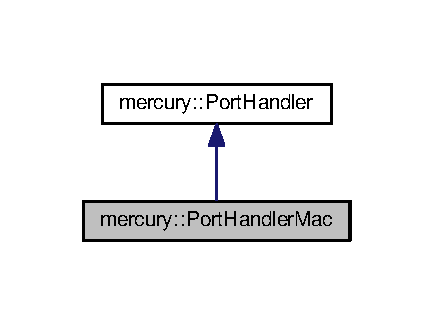
\includegraphics[width=208pt]{classmercury_1_1_port_handler_mac__inherit__graph}
\end{center}
\end{figure}


Collaboration diagram for mercury\+:\+:Port\+Handler\+Mac\+:\nopagebreak
\begin{figure}[H]
\begin{center}
\leavevmode
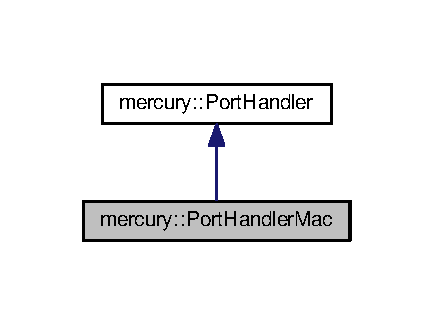
\includegraphics[width=208pt]{classmercury_1_1_port_handler_mac__coll__graph}
\end{center}
\end{figure}
\subsection*{Public Member Functions}
\begin{DoxyCompactItemize}
\item 
\hyperlink{classmercury_1_1_port_handler_mac_a96cd1a75a323cf60fd1d55b377548466}{Port\+Handler\+Mac} (const char $\ast$port\+\_\+name)\hypertarget{classmercury_1_1_port_handler_mac_a96cd1a75a323cf60fd1d55b377548466}{}\label{classmercury_1_1_port_handler_mac_a96cd1a75a323cf60fd1d55b377548466}

\begin{DoxyCompactList}\small\item\em The function that initializes instance of \hyperlink{classmercury_1_1_port_handler}{Port\+Handler} and gets port\+\_\+name  The function initializes instance of \hyperlink{classmercury_1_1_port_handler}{Port\+Handler} and gets port\+\_\+name. \end{DoxyCompactList}\item 
virtual \hyperlink{classmercury_1_1_port_handler_mac_a48c27651e31891a2bf917bdd7aa597c6}{$\sim$\+Port\+Handler\+Mac} ()\hypertarget{classmercury_1_1_port_handler_mac_a48c27651e31891a2bf917bdd7aa597c6}{}\label{classmercury_1_1_port_handler_mac_a48c27651e31891a2bf917bdd7aa597c6}

\begin{DoxyCompactList}\small\item\em The function that closes the port  The function calls \hyperlink{classmercury_1_1_port_handler_mac_aa442d4db9097cd2c5ebf8477d13c0c11}{Port\+Handler\+Mac\+::close\+Port()} to close the port. \end{DoxyCompactList}\item 
bool \hyperlink{classmercury_1_1_port_handler_mac_a572562910975b8ffaf8dd025242dcc9a}{open\+Port} ()
\begin{DoxyCompactList}\small\item\em The function that opens the port  The function calls \hyperlink{classmercury_1_1_port_handler_mac_a05773915cdf00fa5357e4c08e390d556}{Port\+Handler\+Mac\+::set\+Baud\+Rate()} to open the port. \end{DoxyCompactList}\item 
void \hyperlink{classmercury_1_1_port_handler_mac_aa442d4db9097cd2c5ebf8477d13c0c11}{close\+Port} ()\hypertarget{classmercury_1_1_port_handler_mac_aa442d4db9097cd2c5ebf8477d13c0c11}{}\label{classmercury_1_1_port_handler_mac_aa442d4db9097cd2c5ebf8477d13c0c11}

\begin{DoxyCompactList}\small\item\em The function that closes the port  The function closes the port. \end{DoxyCompactList}\item 
void \hyperlink{classmercury_1_1_port_handler_mac_a1a39aa0a85634dfa52d8df9c9ba7d837}{clear\+Port} ()\hypertarget{classmercury_1_1_port_handler_mac_a1a39aa0a85634dfa52d8df9c9ba7d837}{}\label{classmercury_1_1_port_handler_mac_a1a39aa0a85634dfa52d8df9c9ba7d837}

\begin{DoxyCompactList}\small\item\em The function that clears the port  The function clears the port. \end{DoxyCompactList}\item 
void \hyperlink{classmercury_1_1_port_handler_mac_aa5e1d5f8821e11bb5e4dd6aac1f52ec7}{set\+Port\+Name} (const char $\ast$port\+\_\+name)
\begin{DoxyCompactList}\small\item\em The function that sets port name into the port handler  The function sets port name into the port handler. \end{DoxyCompactList}\item 
char $\ast$ \hyperlink{classmercury_1_1_port_handler_mac_a447bb156aedd4ebb1ef845c9e8225536}{get\+Port\+Name} ()
\begin{DoxyCompactList}\small\item\em The function that returns port name set into the port handler  The function returns current port name set into the port handler. \end{DoxyCompactList}\item 
bool \hyperlink{classmercury_1_1_port_handler_mac_a05773915cdf00fa5357e4c08e390d556}{set\+Baud\+Rate} (const int baudrate)
\begin{DoxyCompactList}\small\item\em The function that sets baudrate into the port handler  The function sets baudrate into the port handler. \end{DoxyCompactList}\item 
int \hyperlink{classmercury_1_1_port_handler_mac_ad26a25fed3e7729fd463ebfc96935f1a}{get\+Baud\+Rate} ()
\begin{DoxyCompactList}\small\item\em The function that returns current baudrate set into the port handler  The function returns current baudrate set into the port handler. \end{DoxyCompactList}\item 
int \hyperlink{classmercury_1_1_port_handler_mac_a1b3476c05493aa3226c808825140bf9d}{get\+Bytes\+Available} ()
\begin{DoxyCompactList}\small\item\em The function that checks how much bytes are able to be read from the port buffer  The function checks how much bytes are able to be read from the port buffer  and returns the number. \end{DoxyCompactList}\item 
int \hyperlink{classmercury_1_1_port_handler_mac_a142ad8aa88110a73e2a672bce6bea39e}{read\+Port} (uint8\+\_\+t $\ast$packet, int length)
\begin{DoxyCompactList}\small\item\em The function that reads bytes from the port buffer  The function gets bytes from the port buffer,  and returns a number of bytes read. \end{DoxyCompactList}\item 
int \hyperlink{classmercury_1_1_port_handler_mac_a1a8fb2f94a1eecd4b03d3bfa961c8a32}{write\+Port} (uint8\+\_\+t $\ast$packet, int length)
\begin{DoxyCompactList}\small\item\em The function that writes bytes on the port buffer  The function writes bytes on the port buffer,  and returns a number of bytes which are successfully written. \end{DoxyCompactList}\item 
void \hyperlink{classmercury_1_1_port_handler_mac_aafe74268affe3e64399da08baae6732e}{set\+Packet\+Timeout} (uint16\+\_\+t packet\+\_\+length)
\begin{DoxyCompactList}\small\item\em The function that sets and starts stopwatch for watching packet timeout  The function sets the stopwatch by getting current time and the time of packet timeout with packet\+\_\+length. \end{DoxyCompactList}\item 
void \hyperlink{classmercury_1_1_port_handler_mac_a4c765a51cd5ef9a8310c0a7edae55caf}{set\+Packet\+Timeout} (double msec)
\begin{DoxyCompactList}\small\item\em The function that sets and starts stopwatch for watching packet timeout  The function sets the stopwatch by getting current time and the time of packet timeout with msec. \end{DoxyCompactList}\item 
bool \hyperlink{classmercury_1_1_port_handler_mac_add5e9c4f7edf811a1105b9e77cbe3469}{is\+Packet\+Timeout} ()\hypertarget{classmercury_1_1_port_handler_mac_add5e9c4f7edf811a1105b9e77cbe3469}{}\label{classmercury_1_1_port_handler_mac_add5e9c4f7edf811a1105b9e77cbe3469}

\begin{DoxyCompactList}\small\item\em The function that checks whether packet timeout is occurred  The function checks whether current time is passed by the time of packet timeout from the time set by \hyperlink{classmercury_1_1_port_handler_mac_aafe74268affe3e64399da08baae6732e}{Port\+Handler\+Mac\+::set\+Packet\+Timeout()}. \end{DoxyCompactList}\end{DoxyCompactItemize}
\subsection*{Additional Inherited Members}


\subsection{Detailed Description}
The class for control port in Mac OS. 

\subsection{Member Function Documentation}
\index{mercury\+::\+Port\+Handler\+Mac@{mercury\+::\+Port\+Handler\+Mac}!get\+Baud\+Rate@{get\+Baud\+Rate}}
\index{get\+Baud\+Rate@{get\+Baud\+Rate}!mercury\+::\+Port\+Handler\+Mac@{mercury\+::\+Port\+Handler\+Mac}}
\subsubsection[{\texorpdfstring{get\+Baud\+Rate()}{getBaudRate()}}]{\setlength{\rightskip}{0pt plus 5cm}int mercury\+::\+Port\+Handler\+Mac\+::get\+Baud\+Rate (
\begin{DoxyParamCaption}
{}
\end{DoxyParamCaption}
)\hspace{0.3cm}{\ttfamily [virtual]}}\hypertarget{classmercury_1_1_port_handler_mac_ad26a25fed3e7729fd463ebfc96935f1a}{}\label{classmercury_1_1_port_handler_mac_ad26a25fed3e7729fd463ebfc96935f1a}


The function that returns current baudrate set into the port handler  The function returns current baudrate set into the port handler. 

\begin{DoxyWarning}{Warning}
Mac OS doesn\textquotesingle{}t support over 230400 bps 
\end{DoxyWarning}
\begin{DoxyReturn}{Returns}
Baudrate 
\end{DoxyReturn}


Implements \hyperlink{classmercury_1_1_port_handler_a686c731714c095ac194847cd585643ea}{mercury\+::\+Port\+Handler}.

\index{mercury\+::\+Port\+Handler\+Mac@{mercury\+::\+Port\+Handler\+Mac}!get\+Bytes\+Available@{get\+Bytes\+Available}}
\index{get\+Bytes\+Available@{get\+Bytes\+Available}!mercury\+::\+Port\+Handler\+Mac@{mercury\+::\+Port\+Handler\+Mac}}
\subsubsection[{\texorpdfstring{get\+Bytes\+Available()}{getBytesAvailable()}}]{\setlength{\rightskip}{0pt plus 5cm}int mercury\+::\+Port\+Handler\+Mac\+::get\+Bytes\+Available (
\begin{DoxyParamCaption}
{}
\end{DoxyParamCaption}
)\hspace{0.3cm}{\ttfamily [virtual]}}\hypertarget{classmercury_1_1_port_handler_mac_a1b3476c05493aa3226c808825140bf9d}{}\label{classmercury_1_1_port_handler_mac_a1b3476c05493aa3226c808825140bf9d}


The function that checks how much bytes are able to be read from the port buffer  The function checks how much bytes are able to be read from the port buffer  and returns the number. 

\begin{DoxyReturn}{Returns}
Length of read-\/able bytes in the port buffer 
\end{DoxyReturn}


Implements \hyperlink{classmercury_1_1_port_handler_a2c0a25741b4b8d15e19e619ed7b5a148}{mercury\+::\+Port\+Handler}.

\index{mercury\+::\+Port\+Handler\+Mac@{mercury\+::\+Port\+Handler\+Mac}!get\+Port\+Name@{get\+Port\+Name}}
\index{get\+Port\+Name@{get\+Port\+Name}!mercury\+::\+Port\+Handler\+Mac@{mercury\+::\+Port\+Handler\+Mac}}
\subsubsection[{\texorpdfstring{get\+Port\+Name()}{getPortName()}}]{\setlength{\rightskip}{0pt plus 5cm}char$\ast$ mercury\+::\+Port\+Handler\+Mac\+::get\+Port\+Name (
\begin{DoxyParamCaption}
{}
\end{DoxyParamCaption}
)\hspace{0.3cm}{\ttfamily [virtual]}}\hypertarget{classmercury_1_1_port_handler_mac_a447bb156aedd4ebb1ef845c9e8225536}{}\label{classmercury_1_1_port_handler_mac_a447bb156aedd4ebb1ef845c9e8225536}


The function that returns port name set into the port handler  The function returns current port name set into the port handler. 

\begin{DoxyReturn}{Returns}
Port name 
\end{DoxyReturn}


Implements \hyperlink{classmercury_1_1_port_handler_ab6e0df491f6a6b4f927401e60c0c9c5c}{mercury\+::\+Port\+Handler}.

\index{mercury\+::\+Port\+Handler\+Mac@{mercury\+::\+Port\+Handler\+Mac}!open\+Port@{open\+Port}}
\index{open\+Port@{open\+Port}!mercury\+::\+Port\+Handler\+Mac@{mercury\+::\+Port\+Handler\+Mac}}
\subsubsection[{\texorpdfstring{open\+Port()}{openPort()}}]{\setlength{\rightskip}{0pt plus 5cm}bool mercury\+::\+Port\+Handler\+Mac\+::open\+Port (
\begin{DoxyParamCaption}
{}
\end{DoxyParamCaption}
)\hspace{0.3cm}{\ttfamily [virtual]}}\hypertarget{classmercury_1_1_port_handler_mac_a572562910975b8ffaf8dd025242dcc9a}{}\label{classmercury_1_1_port_handler_mac_a572562910975b8ffaf8dd025242dcc9a}


The function that opens the port  The function calls \hyperlink{classmercury_1_1_port_handler_mac_a05773915cdf00fa5357e4c08e390d556}{Port\+Handler\+Mac\+::set\+Baud\+Rate()} to open the port. 

\begin{DoxyReturn}{Returns}
communication results which come from \hyperlink{classmercury_1_1_port_handler_mac_a05773915cdf00fa5357e4c08e390d556}{Port\+Handler\+Mac\+::set\+Baud\+Rate()} 
\end{DoxyReturn}


Implements \hyperlink{classmercury_1_1_port_handler_a5f65f9a73969cc170582da2d0e11f510}{mercury\+::\+Port\+Handler}.

\index{mercury\+::\+Port\+Handler\+Mac@{mercury\+::\+Port\+Handler\+Mac}!read\+Port@{read\+Port}}
\index{read\+Port@{read\+Port}!mercury\+::\+Port\+Handler\+Mac@{mercury\+::\+Port\+Handler\+Mac}}
\subsubsection[{\texorpdfstring{read\+Port(uint8\+\_\+t $\ast$packet, int length)}{readPort(uint8_t *packet, int length)}}]{\setlength{\rightskip}{0pt plus 5cm}int mercury\+::\+Port\+Handler\+Mac\+::read\+Port (
\begin{DoxyParamCaption}
\item[{uint8\+\_\+t $\ast$}]{packet, }
\item[{int}]{length}
\end{DoxyParamCaption}
)\hspace{0.3cm}{\ttfamily [virtual]}}\hypertarget{classmercury_1_1_port_handler_mac_a142ad8aa88110a73e2a672bce6bea39e}{}\label{classmercury_1_1_port_handler_mac_a142ad8aa88110a73e2a672bce6bea39e}


The function that reads bytes from the port buffer  The function gets bytes from the port buffer,  and returns a number of bytes read. 


\begin{DoxyParams}{Parameters}
{\em packet} & Buffer for the packet received \\
\hline
{\em length} & Length of the buffer for read \\
\hline
\end{DoxyParams}
\begin{DoxyReturn}{Returns}
-\/1 

when error was occurred 

or Length of bytes read 
\end{DoxyReturn}


Implements \hyperlink{classmercury_1_1_port_handler_afa6f52d7b95c5ffd8f0c92477d517c79}{mercury\+::\+Port\+Handler}.

\index{mercury\+::\+Port\+Handler\+Mac@{mercury\+::\+Port\+Handler\+Mac}!set\+Baud\+Rate@{set\+Baud\+Rate}}
\index{set\+Baud\+Rate@{set\+Baud\+Rate}!mercury\+::\+Port\+Handler\+Mac@{mercury\+::\+Port\+Handler\+Mac}}
\subsubsection[{\texorpdfstring{set\+Baud\+Rate(const int baudrate)}{setBaudRate(const int baudrate)}}]{\setlength{\rightskip}{0pt plus 5cm}bool mercury\+::\+Port\+Handler\+Mac\+::set\+Baud\+Rate (
\begin{DoxyParamCaption}
\item[{const int}]{baudrate}
\end{DoxyParamCaption}
)\hspace{0.3cm}{\ttfamily [virtual]}}\hypertarget{classmercury_1_1_port_handler_mac_a05773915cdf00fa5357e4c08e390d556}{}\label{classmercury_1_1_port_handler_mac_a05773915cdf00fa5357e4c08e390d556}


The function that sets baudrate into the port handler  The function sets baudrate into the port handler. 


\begin{DoxyParams}{Parameters}
{\em baudrate} & Baudrate \\
\hline
\end{DoxyParams}
\begin{DoxyReturn}{Returns}
false 

when error was occurred during port opening 

or true 
\end{DoxyReturn}


Implements \hyperlink{classmercury_1_1_port_handler_a663168c32580a532ccb328544565f06d}{mercury\+::\+Port\+Handler}.

\index{mercury\+::\+Port\+Handler\+Mac@{mercury\+::\+Port\+Handler\+Mac}!set\+Packet\+Timeout@{set\+Packet\+Timeout}}
\index{set\+Packet\+Timeout@{set\+Packet\+Timeout}!mercury\+::\+Port\+Handler\+Mac@{mercury\+::\+Port\+Handler\+Mac}}
\subsubsection[{\texorpdfstring{set\+Packet\+Timeout(uint16\+\_\+t packet\+\_\+length)}{setPacketTimeout(uint16_t packet_length)}}]{\setlength{\rightskip}{0pt plus 5cm}void mercury\+::\+Port\+Handler\+Mac\+::set\+Packet\+Timeout (
\begin{DoxyParamCaption}
\item[{uint16\+\_\+t}]{packet\+\_\+length}
\end{DoxyParamCaption}
)\hspace{0.3cm}{\ttfamily [virtual]}}\hypertarget{classmercury_1_1_port_handler_mac_aafe74268affe3e64399da08baae6732e}{}\label{classmercury_1_1_port_handler_mac_aafe74268affe3e64399da08baae6732e}


The function that sets and starts stopwatch for watching packet timeout  The function sets the stopwatch by getting current time and the time of packet timeout with packet\+\_\+length. 


\begin{DoxyParams}{Parameters}
{\em packet\+\_\+length} & Length of the packet expected to be received \\
\hline
\end{DoxyParams}


Implements \hyperlink{classmercury_1_1_port_handler_ae79ec2448529ffc2f1788da26142d164}{mercury\+::\+Port\+Handler}.

\index{mercury\+::\+Port\+Handler\+Mac@{mercury\+::\+Port\+Handler\+Mac}!set\+Packet\+Timeout@{set\+Packet\+Timeout}}
\index{set\+Packet\+Timeout@{set\+Packet\+Timeout}!mercury\+::\+Port\+Handler\+Mac@{mercury\+::\+Port\+Handler\+Mac}}
\subsubsection[{\texorpdfstring{set\+Packet\+Timeout(double msec)}{setPacketTimeout(double msec)}}]{\setlength{\rightskip}{0pt plus 5cm}void mercury\+::\+Port\+Handler\+Mac\+::set\+Packet\+Timeout (
\begin{DoxyParamCaption}
\item[{double}]{msec}
\end{DoxyParamCaption}
)\hspace{0.3cm}{\ttfamily [virtual]}}\hypertarget{classmercury_1_1_port_handler_mac_a4c765a51cd5ef9a8310c0a7edae55caf}{}\label{classmercury_1_1_port_handler_mac_a4c765a51cd5ef9a8310c0a7edae55caf}


The function that sets and starts stopwatch for watching packet timeout  The function sets the stopwatch by getting current time and the time of packet timeout with msec. 


\begin{DoxyParams}{Parameters}
{\em packet\+\_\+length} & Length of the packet expected to be received \\
\hline
\end{DoxyParams}


Implements \hyperlink{classmercury_1_1_port_handler_ae61a4953ef52be49401af210acf820a4}{mercury\+::\+Port\+Handler}.

\index{mercury\+::\+Port\+Handler\+Mac@{mercury\+::\+Port\+Handler\+Mac}!set\+Port\+Name@{set\+Port\+Name}}
\index{set\+Port\+Name@{set\+Port\+Name}!mercury\+::\+Port\+Handler\+Mac@{mercury\+::\+Port\+Handler\+Mac}}
\subsubsection[{\texorpdfstring{set\+Port\+Name(const char $\ast$port\+\_\+name)}{setPortName(const char *port_name)}}]{\setlength{\rightskip}{0pt plus 5cm}void mercury\+::\+Port\+Handler\+Mac\+::set\+Port\+Name (
\begin{DoxyParamCaption}
\item[{const char $\ast$}]{port\+\_\+name}
\end{DoxyParamCaption}
)\hspace{0.3cm}{\ttfamily [virtual]}}\hypertarget{classmercury_1_1_port_handler_mac_aa5e1d5f8821e11bb5e4dd6aac1f52ec7}{}\label{classmercury_1_1_port_handler_mac_aa5e1d5f8821e11bb5e4dd6aac1f52ec7}


The function that sets port name into the port handler  The function sets port name into the port handler. 


\begin{DoxyParams}{Parameters}
{\em port\+\_\+name} & Port name \\
\hline
\end{DoxyParams}


Implements \hyperlink{classmercury_1_1_port_handler_adb0bff39482904066c1bdd7713441e9e}{mercury\+::\+Port\+Handler}.

\index{mercury\+::\+Port\+Handler\+Mac@{mercury\+::\+Port\+Handler\+Mac}!write\+Port@{write\+Port}}
\index{write\+Port@{write\+Port}!mercury\+::\+Port\+Handler\+Mac@{mercury\+::\+Port\+Handler\+Mac}}
\subsubsection[{\texorpdfstring{write\+Port(uint8\+\_\+t $\ast$packet, int length)}{writePort(uint8_t *packet, int length)}}]{\setlength{\rightskip}{0pt plus 5cm}int mercury\+::\+Port\+Handler\+Mac\+::write\+Port (
\begin{DoxyParamCaption}
\item[{uint8\+\_\+t $\ast$}]{packet, }
\item[{int}]{length}
\end{DoxyParamCaption}
)\hspace{0.3cm}{\ttfamily [virtual]}}\hypertarget{classmercury_1_1_port_handler_mac_a1a8fb2f94a1eecd4b03d3bfa961c8a32}{}\label{classmercury_1_1_port_handler_mac_a1a8fb2f94a1eecd4b03d3bfa961c8a32}


The function that writes bytes on the port buffer  The function writes bytes on the port buffer,  and returns a number of bytes which are successfully written. 


\begin{DoxyParams}{Parameters}
{\em packet} & Buffer which would be written on the port buffer \\
\hline
{\em length} & Length of the buffer for write \\
\hline
\end{DoxyParams}
\begin{DoxyReturn}{Returns}
-\/1 

when error was occurred 

or Length of bytes written 
\end{DoxyReturn}


Implements \hyperlink{classmercury_1_1_port_handler_ad26c3a106d6b668b6fae3d2f0afeab9e}{mercury\+::\+Port\+Handler}.



The documentation for this class was generated from the following file\+:\begin{DoxyCompactItemize}
\item 
/home/wigir/dev/software/projects/\+Mercury\+S\+D\+K/c++/include/mercury\+\_\+sdk/port\+\_\+handler\+\_\+mac.\+h\end{DoxyCompactItemize}

\hypertarget{classmercury_1_1_port_handler_windows}{}\section{mercury\+:\+:Port\+Handler\+Windows Class Reference}
\label{classmercury_1_1_port_handler_windows}\index{mercury\+::\+Port\+Handler\+Windows@{mercury\+::\+Port\+Handler\+Windows}}


The class for control port in Windows.  




{\ttfamily \#include $<$port\+\_\+handler\+\_\+windows.\+h$>$}



Inheritance diagram for mercury\+:\+:Port\+Handler\+Windows\+:\nopagebreak
\begin{figure}[H]
\begin{center}
\leavevmode
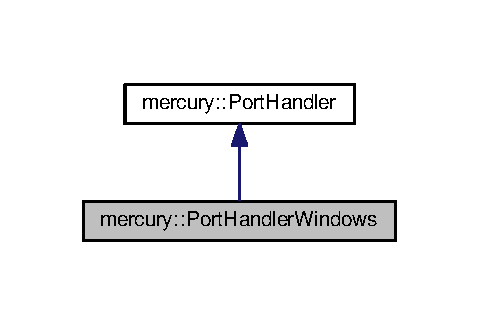
\includegraphics[width=230pt]{classmercury_1_1_port_handler_windows__inherit__graph}
\end{center}
\end{figure}


Collaboration diagram for mercury\+:\+:Port\+Handler\+Windows\+:\nopagebreak
\begin{figure}[H]
\begin{center}
\leavevmode
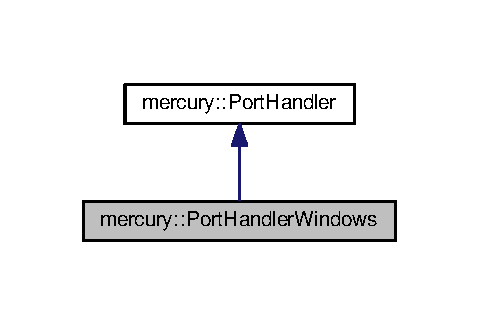
\includegraphics[width=230pt]{classmercury_1_1_port_handler_windows__coll__graph}
\end{center}
\end{figure}
\subsection*{Public Member Functions}
\begin{DoxyCompactItemize}
\item 
\hyperlink{classmercury_1_1_port_handler_windows_aa7849c96f4541fd6d1c139b33902fe24}{Port\+Handler\+Windows} (const char $\ast$port\+\_\+name)\hypertarget{classmercury_1_1_port_handler_windows_aa7849c96f4541fd6d1c139b33902fe24}{}\label{classmercury_1_1_port_handler_windows_aa7849c96f4541fd6d1c139b33902fe24}

\begin{DoxyCompactList}\small\item\em The function that initializes instance of \hyperlink{classmercury_1_1_port_handler}{Port\+Handler} and gets port\+\_\+name  The function initializes instance of \hyperlink{classmercury_1_1_port_handler}{Port\+Handler} and gets port\+\_\+name. \end{DoxyCompactList}\item 
virtual \hyperlink{classmercury_1_1_port_handler_windows_a15b9eb8961f1c19471ccf28b50e44e17}{$\sim$\+Port\+Handler\+Windows} ()\hypertarget{classmercury_1_1_port_handler_windows_a15b9eb8961f1c19471ccf28b50e44e17}{}\label{classmercury_1_1_port_handler_windows_a15b9eb8961f1c19471ccf28b50e44e17}

\begin{DoxyCompactList}\small\item\em The function that closes the port  The function calls \hyperlink{classmercury_1_1_port_handler_windows_a75263b8ac698a2ae302fc68265523463}{Port\+Handler\+Windows\+::close\+Port()} to close the port. \end{DoxyCompactList}\item 
bool \hyperlink{classmercury_1_1_port_handler_windows_adfe63f740bfc82abc6ba720a2c87116b}{open\+Port} ()
\begin{DoxyCompactList}\small\item\em The function that opens the port  The function calls \hyperlink{classmercury_1_1_port_handler_windows_a31dedf26ac2e57cc3cd39f8a3372d2da}{Port\+Handler\+Windows\+::set\+Baud\+Rate()} to open the port. \end{DoxyCompactList}\item 
void \hyperlink{classmercury_1_1_port_handler_windows_a75263b8ac698a2ae302fc68265523463}{close\+Port} ()\hypertarget{classmercury_1_1_port_handler_windows_a75263b8ac698a2ae302fc68265523463}{}\label{classmercury_1_1_port_handler_windows_a75263b8ac698a2ae302fc68265523463}

\begin{DoxyCompactList}\small\item\em The function that closes the port  The function closes the port. \end{DoxyCompactList}\item 
void \hyperlink{classmercury_1_1_port_handler_windows_a139357916c945845a6b100106285eb83}{clear\+Port} ()\hypertarget{classmercury_1_1_port_handler_windows_a139357916c945845a6b100106285eb83}{}\label{classmercury_1_1_port_handler_windows_a139357916c945845a6b100106285eb83}

\begin{DoxyCompactList}\small\item\em The function that clears the port  The function clears the port. \end{DoxyCompactList}\item 
void \hyperlink{classmercury_1_1_port_handler_windows_ab4dc705daf44c4688dca7f2ee7dd3747}{set\+Port\+Name} (const char $\ast$port\+\_\+name)
\begin{DoxyCompactList}\small\item\em The function that sets port name into the port handler  The function sets port name into the port handler. \end{DoxyCompactList}\item 
char $\ast$ \hyperlink{classmercury_1_1_port_handler_windows_acabc8f26d7e894fc993b5b991f7f8ab4}{get\+Port\+Name} ()
\begin{DoxyCompactList}\small\item\em The function that returns port name set into the port handler  The function returns current port name set into the port handler. \end{DoxyCompactList}\item 
bool \hyperlink{classmercury_1_1_port_handler_windows_a31dedf26ac2e57cc3cd39f8a3372d2da}{set\+Baud\+Rate} (const int baudrate)
\begin{DoxyCompactList}\small\item\em The function that sets baudrate into the port handler  The function sets baudrate into the port handler. \end{DoxyCompactList}\item 
int \hyperlink{classmercury_1_1_port_handler_windows_a348830218ff48aab3c8f1e56c96d852c}{get\+Baud\+Rate} ()
\begin{DoxyCompactList}\small\item\em The function that returns current baudrate set into the port handler  The function returns current baudrate set into the port handler. \end{DoxyCompactList}\item 
int \hyperlink{classmercury_1_1_port_handler_windows_a96f874b469b2565a99e0686bde6ad877}{get\+Bytes\+Available} ()
\begin{DoxyCompactList}\small\item\em The function that checks how much bytes are able to be read from the port buffer  The function checks how much bytes are able to be read from the port buffer  and returns the number. \end{DoxyCompactList}\item 
int \hyperlink{classmercury_1_1_port_handler_windows_af86bc8437461da934d84cd205a252d9f}{read\+Port} (uint8\+\_\+t $\ast$packet, int length)
\begin{DoxyCompactList}\small\item\em The function that reads bytes from the port buffer  The function gets bytes from the port buffer,  and returns a number of bytes read. \end{DoxyCompactList}\item 
int \hyperlink{classmercury_1_1_port_handler_windows_a4aef1e4a583ea4194afc5a926209e3a3}{write\+Port} (uint8\+\_\+t $\ast$packet, int length)
\begin{DoxyCompactList}\small\item\em The function that writes bytes on the port buffer  The function writes bytes on the port buffer,  and returns a number of bytes which are successfully written. \end{DoxyCompactList}\item 
void \hyperlink{classmercury_1_1_port_handler_windows_aab80ca949581a85b60e985bb31352875}{set\+Packet\+Timeout} (uint16\+\_\+t packet\+\_\+length)
\begin{DoxyCompactList}\small\item\em The function that sets and starts stopwatch for watching packet timeout  The function sets the stopwatch by getting current time and the time of packet timeout with packet\+\_\+length. \end{DoxyCompactList}\item 
void \hyperlink{classmercury_1_1_port_handler_windows_ac1e4413b63e3c5bd8320df864257543e}{set\+Packet\+Timeout} (double msec)
\begin{DoxyCompactList}\small\item\em The function that sets and starts stopwatch for watching packet timeout  The function sets the stopwatch by getting current time and the time of packet timeout with msec. \end{DoxyCompactList}\item 
bool \hyperlink{classmercury_1_1_port_handler_windows_ab8c72fb39e2632f1c07d5be6f313e0eb}{is\+Packet\+Timeout} ()\hypertarget{classmercury_1_1_port_handler_windows_ab8c72fb39e2632f1c07d5be6f313e0eb}{}\label{classmercury_1_1_port_handler_windows_ab8c72fb39e2632f1c07d5be6f313e0eb}

\begin{DoxyCompactList}\small\item\em The function that checks whether packet timeout is occurred  The function checks whether current time is passed by the time of packet timeout from the time set by \hyperlink{classmercury_1_1_port_handler_windows_aab80ca949581a85b60e985bb31352875}{Port\+Handler\+Windows\+::set\+Packet\+Timeout()}. \end{DoxyCompactList}\end{DoxyCompactItemize}
\subsection*{Additional Inherited Members}


\subsection{Detailed Description}
The class for control port in Windows. 

\subsection{Member Function Documentation}
\index{mercury\+::\+Port\+Handler\+Windows@{mercury\+::\+Port\+Handler\+Windows}!get\+Baud\+Rate@{get\+Baud\+Rate}}
\index{get\+Baud\+Rate@{get\+Baud\+Rate}!mercury\+::\+Port\+Handler\+Windows@{mercury\+::\+Port\+Handler\+Windows}}
\subsubsection[{\texorpdfstring{get\+Baud\+Rate()}{getBaudRate()}}]{\setlength{\rightskip}{0pt plus 5cm}int mercury\+::\+Port\+Handler\+Windows\+::get\+Baud\+Rate (
\begin{DoxyParamCaption}
{}
\end{DoxyParamCaption}
)\hspace{0.3cm}{\ttfamily [virtual]}}\hypertarget{classmercury_1_1_port_handler_windows_a348830218ff48aab3c8f1e56c96d852c}{}\label{classmercury_1_1_port_handler_windows_a348830218ff48aab3c8f1e56c96d852c}


The function that returns current baudrate set into the port handler  The function returns current baudrate set into the port handler. 

\begin{DoxyReturn}{Returns}
Baudrate 
\end{DoxyReturn}


Implements \hyperlink{classmercury_1_1_port_handler_a686c731714c095ac194847cd585643ea}{mercury\+::\+Port\+Handler}.

\index{mercury\+::\+Port\+Handler\+Windows@{mercury\+::\+Port\+Handler\+Windows}!get\+Bytes\+Available@{get\+Bytes\+Available}}
\index{get\+Bytes\+Available@{get\+Bytes\+Available}!mercury\+::\+Port\+Handler\+Windows@{mercury\+::\+Port\+Handler\+Windows}}
\subsubsection[{\texorpdfstring{get\+Bytes\+Available()}{getBytesAvailable()}}]{\setlength{\rightskip}{0pt plus 5cm}int mercury\+::\+Port\+Handler\+Windows\+::get\+Bytes\+Available (
\begin{DoxyParamCaption}
{}
\end{DoxyParamCaption}
)\hspace{0.3cm}{\ttfamily [virtual]}}\hypertarget{classmercury_1_1_port_handler_windows_a96f874b469b2565a99e0686bde6ad877}{}\label{classmercury_1_1_port_handler_windows_a96f874b469b2565a99e0686bde6ad877}


The function that checks how much bytes are able to be read from the port buffer  The function checks how much bytes are able to be read from the port buffer  and returns the number. 

\begin{DoxyReturn}{Returns}
Length of read-\/able bytes in the port buffer 
\end{DoxyReturn}


Implements \hyperlink{classmercury_1_1_port_handler_a2c0a25741b4b8d15e19e619ed7b5a148}{mercury\+::\+Port\+Handler}.

\index{mercury\+::\+Port\+Handler\+Windows@{mercury\+::\+Port\+Handler\+Windows}!get\+Port\+Name@{get\+Port\+Name}}
\index{get\+Port\+Name@{get\+Port\+Name}!mercury\+::\+Port\+Handler\+Windows@{mercury\+::\+Port\+Handler\+Windows}}
\subsubsection[{\texorpdfstring{get\+Port\+Name()}{getPortName()}}]{\setlength{\rightskip}{0pt plus 5cm}char$\ast$ mercury\+::\+Port\+Handler\+Windows\+::get\+Port\+Name (
\begin{DoxyParamCaption}
{}
\end{DoxyParamCaption}
)\hspace{0.3cm}{\ttfamily [virtual]}}\hypertarget{classmercury_1_1_port_handler_windows_acabc8f26d7e894fc993b5b991f7f8ab4}{}\label{classmercury_1_1_port_handler_windows_acabc8f26d7e894fc993b5b991f7f8ab4}


The function that returns port name set into the port handler  The function returns current port name set into the port handler. 

\begin{DoxyReturn}{Returns}
Port name 
\end{DoxyReturn}


Implements \hyperlink{classmercury_1_1_port_handler_ab6e0df491f6a6b4f927401e60c0c9c5c}{mercury\+::\+Port\+Handler}.

\index{mercury\+::\+Port\+Handler\+Windows@{mercury\+::\+Port\+Handler\+Windows}!open\+Port@{open\+Port}}
\index{open\+Port@{open\+Port}!mercury\+::\+Port\+Handler\+Windows@{mercury\+::\+Port\+Handler\+Windows}}
\subsubsection[{\texorpdfstring{open\+Port()}{openPort()}}]{\setlength{\rightskip}{0pt plus 5cm}bool mercury\+::\+Port\+Handler\+Windows\+::open\+Port (
\begin{DoxyParamCaption}
{}
\end{DoxyParamCaption}
)\hspace{0.3cm}{\ttfamily [virtual]}}\hypertarget{classmercury_1_1_port_handler_windows_adfe63f740bfc82abc6ba720a2c87116b}{}\label{classmercury_1_1_port_handler_windows_adfe63f740bfc82abc6ba720a2c87116b}


The function that opens the port  The function calls \hyperlink{classmercury_1_1_port_handler_windows_a31dedf26ac2e57cc3cd39f8a3372d2da}{Port\+Handler\+Windows\+::set\+Baud\+Rate()} to open the port. 

\begin{DoxyReturn}{Returns}
communication results which come from \hyperlink{classmercury_1_1_port_handler_windows_a31dedf26ac2e57cc3cd39f8a3372d2da}{Port\+Handler\+Windows\+::set\+Baud\+Rate()} 
\end{DoxyReturn}


Implements \hyperlink{classmercury_1_1_port_handler_a5f65f9a73969cc170582da2d0e11f510}{mercury\+::\+Port\+Handler}.

\index{mercury\+::\+Port\+Handler\+Windows@{mercury\+::\+Port\+Handler\+Windows}!read\+Port@{read\+Port}}
\index{read\+Port@{read\+Port}!mercury\+::\+Port\+Handler\+Windows@{mercury\+::\+Port\+Handler\+Windows}}
\subsubsection[{\texorpdfstring{read\+Port(uint8\+\_\+t $\ast$packet, int length)}{readPort(uint8_t *packet, int length)}}]{\setlength{\rightskip}{0pt plus 5cm}int mercury\+::\+Port\+Handler\+Windows\+::read\+Port (
\begin{DoxyParamCaption}
\item[{uint8\+\_\+t $\ast$}]{packet, }
\item[{int}]{length}
\end{DoxyParamCaption}
)\hspace{0.3cm}{\ttfamily [virtual]}}\hypertarget{classmercury_1_1_port_handler_windows_af86bc8437461da934d84cd205a252d9f}{}\label{classmercury_1_1_port_handler_windows_af86bc8437461da934d84cd205a252d9f}


The function that reads bytes from the port buffer  The function gets bytes from the port buffer,  and returns a number of bytes read. 


\begin{DoxyParams}{Parameters}
{\em packet} & Buffer for the packet received \\
\hline
{\em length} & Length of the buffer for read \\
\hline
\end{DoxyParams}
\begin{DoxyReturn}{Returns}
-\/1 

when error was occurred 

or Length of bytes read 
\end{DoxyReturn}


Implements \hyperlink{classmercury_1_1_port_handler_afa6f52d7b95c5ffd8f0c92477d517c79}{mercury\+::\+Port\+Handler}.

\index{mercury\+::\+Port\+Handler\+Windows@{mercury\+::\+Port\+Handler\+Windows}!set\+Baud\+Rate@{set\+Baud\+Rate}}
\index{set\+Baud\+Rate@{set\+Baud\+Rate}!mercury\+::\+Port\+Handler\+Windows@{mercury\+::\+Port\+Handler\+Windows}}
\subsubsection[{\texorpdfstring{set\+Baud\+Rate(const int baudrate)}{setBaudRate(const int baudrate)}}]{\setlength{\rightskip}{0pt plus 5cm}bool mercury\+::\+Port\+Handler\+Windows\+::set\+Baud\+Rate (
\begin{DoxyParamCaption}
\item[{const int}]{baudrate}
\end{DoxyParamCaption}
)\hspace{0.3cm}{\ttfamily [virtual]}}\hypertarget{classmercury_1_1_port_handler_windows_a31dedf26ac2e57cc3cd39f8a3372d2da}{}\label{classmercury_1_1_port_handler_windows_a31dedf26ac2e57cc3cd39f8a3372d2da}


The function that sets baudrate into the port handler  The function sets baudrate into the port handler. 


\begin{DoxyParams}{Parameters}
{\em baudrate} & Baudrate \\
\hline
\end{DoxyParams}
\begin{DoxyReturn}{Returns}
false 

when error was occurred during port opening 

or true 
\end{DoxyReturn}


Implements \hyperlink{classmercury_1_1_port_handler_a663168c32580a532ccb328544565f06d}{mercury\+::\+Port\+Handler}.

\index{mercury\+::\+Port\+Handler\+Windows@{mercury\+::\+Port\+Handler\+Windows}!set\+Packet\+Timeout@{set\+Packet\+Timeout}}
\index{set\+Packet\+Timeout@{set\+Packet\+Timeout}!mercury\+::\+Port\+Handler\+Windows@{mercury\+::\+Port\+Handler\+Windows}}
\subsubsection[{\texorpdfstring{set\+Packet\+Timeout(uint16\+\_\+t packet\+\_\+length)}{setPacketTimeout(uint16_t packet_length)}}]{\setlength{\rightskip}{0pt plus 5cm}void mercury\+::\+Port\+Handler\+Windows\+::set\+Packet\+Timeout (
\begin{DoxyParamCaption}
\item[{uint16\+\_\+t}]{packet\+\_\+length}
\end{DoxyParamCaption}
)\hspace{0.3cm}{\ttfamily [virtual]}}\hypertarget{classmercury_1_1_port_handler_windows_aab80ca949581a85b60e985bb31352875}{}\label{classmercury_1_1_port_handler_windows_aab80ca949581a85b60e985bb31352875}


The function that sets and starts stopwatch for watching packet timeout  The function sets the stopwatch by getting current time and the time of packet timeout with packet\+\_\+length. 


\begin{DoxyParams}{Parameters}
{\em packet\+\_\+length} & Length of the packet expected to be received \\
\hline
\end{DoxyParams}


Implements \hyperlink{classmercury_1_1_port_handler_ae79ec2448529ffc2f1788da26142d164}{mercury\+::\+Port\+Handler}.

\index{mercury\+::\+Port\+Handler\+Windows@{mercury\+::\+Port\+Handler\+Windows}!set\+Packet\+Timeout@{set\+Packet\+Timeout}}
\index{set\+Packet\+Timeout@{set\+Packet\+Timeout}!mercury\+::\+Port\+Handler\+Windows@{mercury\+::\+Port\+Handler\+Windows}}
\subsubsection[{\texorpdfstring{set\+Packet\+Timeout(double msec)}{setPacketTimeout(double msec)}}]{\setlength{\rightskip}{0pt plus 5cm}void mercury\+::\+Port\+Handler\+Windows\+::set\+Packet\+Timeout (
\begin{DoxyParamCaption}
\item[{double}]{msec}
\end{DoxyParamCaption}
)\hspace{0.3cm}{\ttfamily [virtual]}}\hypertarget{classmercury_1_1_port_handler_windows_ac1e4413b63e3c5bd8320df864257543e}{}\label{classmercury_1_1_port_handler_windows_ac1e4413b63e3c5bd8320df864257543e}


The function that sets and starts stopwatch for watching packet timeout  The function sets the stopwatch by getting current time and the time of packet timeout with msec. 


\begin{DoxyParams}{Parameters}
{\em packet\+\_\+length} & Length of the packet expected to be received \\
\hline
\end{DoxyParams}


Implements \hyperlink{classmercury_1_1_port_handler_ae61a4953ef52be49401af210acf820a4}{mercury\+::\+Port\+Handler}.

\index{mercury\+::\+Port\+Handler\+Windows@{mercury\+::\+Port\+Handler\+Windows}!set\+Port\+Name@{set\+Port\+Name}}
\index{set\+Port\+Name@{set\+Port\+Name}!mercury\+::\+Port\+Handler\+Windows@{mercury\+::\+Port\+Handler\+Windows}}
\subsubsection[{\texorpdfstring{set\+Port\+Name(const char $\ast$port\+\_\+name)}{setPortName(const char *port_name)}}]{\setlength{\rightskip}{0pt plus 5cm}void mercury\+::\+Port\+Handler\+Windows\+::set\+Port\+Name (
\begin{DoxyParamCaption}
\item[{const char $\ast$}]{port\+\_\+name}
\end{DoxyParamCaption}
)\hspace{0.3cm}{\ttfamily [virtual]}}\hypertarget{classmercury_1_1_port_handler_windows_ab4dc705daf44c4688dca7f2ee7dd3747}{}\label{classmercury_1_1_port_handler_windows_ab4dc705daf44c4688dca7f2ee7dd3747}


The function that sets port name into the port handler  The function sets port name into the port handler. 


\begin{DoxyParams}{Parameters}
{\em port\+\_\+name} & Port name \\
\hline
\end{DoxyParams}


Implements \hyperlink{classmercury_1_1_port_handler_adb0bff39482904066c1bdd7713441e9e}{mercury\+::\+Port\+Handler}.

\index{mercury\+::\+Port\+Handler\+Windows@{mercury\+::\+Port\+Handler\+Windows}!write\+Port@{write\+Port}}
\index{write\+Port@{write\+Port}!mercury\+::\+Port\+Handler\+Windows@{mercury\+::\+Port\+Handler\+Windows}}
\subsubsection[{\texorpdfstring{write\+Port(uint8\+\_\+t $\ast$packet, int length)}{writePort(uint8_t *packet, int length)}}]{\setlength{\rightskip}{0pt plus 5cm}int mercury\+::\+Port\+Handler\+Windows\+::write\+Port (
\begin{DoxyParamCaption}
\item[{uint8\+\_\+t $\ast$}]{packet, }
\item[{int}]{length}
\end{DoxyParamCaption}
)\hspace{0.3cm}{\ttfamily [virtual]}}\hypertarget{classmercury_1_1_port_handler_windows_a4aef1e4a583ea4194afc5a926209e3a3}{}\label{classmercury_1_1_port_handler_windows_a4aef1e4a583ea4194afc5a926209e3a3}


The function that writes bytes on the port buffer  The function writes bytes on the port buffer,  and returns a number of bytes which are successfully written. 


\begin{DoxyParams}{Parameters}
{\em packet} & Buffer which would be written on the port buffer \\
\hline
{\em length} & Length of the buffer for write \\
\hline
\end{DoxyParams}
\begin{DoxyReturn}{Returns}
-\/1 

when error was occurred 

or Length of bytes written 
\end{DoxyReturn}


Implements \hyperlink{classmercury_1_1_port_handler_ad26c3a106d6b668b6fae3d2f0afeab9e}{mercury\+::\+Port\+Handler}.



The documentation for this class was generated from the following file\+:\begin{DoxyCompactItemize}
\item 
/home/wigir/dev/software/projects/\+Mercury\+S\+D\+K/c++/include/mercury\+\_\+sdk/port\+\_\+handler\+\_\+windows.\+h\end{DoxyCompactItemize}

\hypertarget{classmercury_1_1_protocol_packet_handler}{}\section{mercury\+:\+:Protocol\+Packet\+Handler Class Reference}
\label{classmercury_1_1_protocol_packet_handler}\index{mercury\+::\+Protocol\+Packet\+Handler@{mercury\+::\+Protocol\+Packet\+Handler}}


The class for control Mercury by using Protocol.\+0.  




{\ttfamily \#include $<$protocol\+\_\+packet\+\_\+handler.\+h$>$}



Inheritance diagram for mercury\+:\+:Protocol\+Packet\+Handler\+:\nopagebreak
\begin{figure}[H]
\begin{center}
\leavevmode
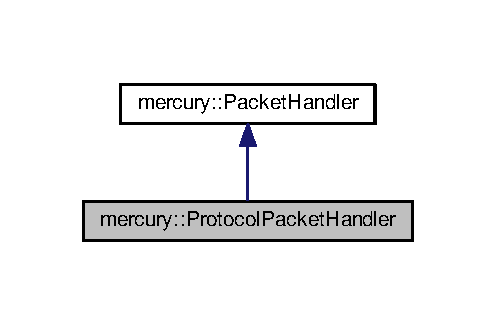
\includegraphics[width=238pt]{classmercury_1_1_protocol_packet_handler__inherit__graph}
\end{center}
\end{figure}


Collaboration diagram for mercury\+:\+:Protocol\+Packet\+Handler\+:\nopagebreak
\begin{figure}[H]
\begin{center}
\leavevmode
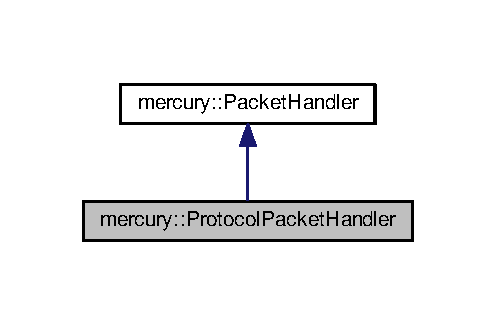
\includegraphics[width=238pt]{classmercury_1_1_protocol_packet_handler__coll__graph}
\end{center}
\end{figure}
\subsection*{Public Member Functions}
\begin{DoxyCompactItemize}
\item 
float \hyperlink{classmercury_1_1_protocol_packet_handler_a79099f3c0ebc35a9198ca88ab3bfb284}{get\+Protocol\+Version} ()
\begin{DoxyCompactList}\small\item\em The function that returns Protocol version used in \hyperlink{classmercury_1_1_protocol_packet_handler}{Protocol\+Packet\+Handler} (1.\+0) \end{DoxyCompactList}\item 
const char $\ast$ \hyperlink{classmercury_1_1_protocol_packet_handler_a9c963a7033794c15b4d51ccf7455897f}{get\+Tx\+Rx\+Result} (int result)
\begin{DoxyCompactList}\small\item\em The function that gets description of communication result. \end{DoxyCompactList}\item 
const char $\ast$ \hyperlink{classmercury_1_1_protocol_packet_handler_a0567896a3552cd6bea62e81f2b42741e}{get\+Rx\+Packet\+Error} (uint8\+\_\+t error)
\begin{DoxyCompactList}\small\item\em The function that gets description of hardware error. \end{DoxyCompactList}\item 
int \hyperlink{classmercury_1_1_protocol_packet_handler_a245f01395d9684bc58788e8a06de3ffc}{tx\+Packet} (\hyperlink{classmercury_1_1_port_handler}{Port\+Handler} $\ast$port, uint8\+\_\+t $\ast$txpacket)
\begin{DoxyCompactList}\small\item\em The function that transmits the instruction packet txpacket via \hyperlink{classmercury_1_1_port_handler}{Port\+Handler} port.  The function clears the port buffer by \hyperlink{classmercury_1_1_port_handler_accf37c8838c1ce3042a0127ceeb89c48}{Port\+Handler\+::clear\+Port()} function,  then transmits txpacket by \hyperlink{classmercury_1_1_port_handler_ad26c3a106d6b668b6fae3d2f0afeab9e}{Port\+Handler\+::write\+Port()} function.  The function activates only when the port is not busy and when the packet is already written on the port buffer. \end{DoxyCompactList}\item 
int \hyperlink{classmercury_1_1_protocol_packet_handler_a4d124ca43f6a2178497eaaabb9e5907b}{rx\+Packet} (\hyperlink{classmercury_1_1_port_handler}{Port\+Handler} $\ast$port, uint8\+\_\+t $\ast$rxpacket)
\begin{DoxyCompactList}\small\item\em The function that receives packet (rxpacket) during designated time via \hyperlink{classmercury_1_1_port_handler}{Port\+Handler} port  The function repeatedly tries to receive rxpacket by \hyperlink{classmercury_1_1_port_handler_afa6f52d7b95c5ffd8f0c92477d517c79}{Port\+Handler\+::read\+Port()} function.  It breaks out  when \hyperlink{classmercury_1_1_port_handler_a6733438255ede3d34738842e10cd8fc2}{Port\+Handler\+::is\+Packet\+Timeout()} shows the timeout,  when rxpacket seemed as corrupted, or  when nothing received. \end{DoxyCompactList}\item 
int \hyperlink{classmercury_1_1_protocol_packet_handler_a68b02f23af616886d0795ea12debd613}{tx\+Rx\+Packet} (\hyperlink{classmercury_1_1_port_handler}{Port\+Handler} $\ast$port, uint8\+\_\+t $\ast$txpacket, uint8\+\_\+t $\ast$rxpacket, uint8\+\_\+t $\ast$error=0)
\begin{DoxyCompactList}\small\item\em The function that transmits packet (txpacket) and receives packet (rxpacket) during designated time via \hyperlink{classmercury_1_1_port_handler}{Port\+Handler} port  The function calls \hyperlink{classmercury_1_1_protocol_packet_handler_a245f01395d9684bc58788e8a06de3ffc}{Protocol\+Packet\+Handler\+::tx\+Packet()},  and calls \hyperlink{classmercury_1_1_protocol_packet_handler_a4d124ca43f6a2178497eaaabb9e5907b}{Protocol\+Packet\+Handler\+::rx\+Packet()} if it succeeds \hyperlink{classmercury_1_1_protocol_packet_handler_a245f01395d9684bc58788e8a06de3ffc}{Protocol\+Packet\+Handler\+::tx\+Packet()}.  It breaks out  when it fails \hyperlink{classmercury_1_1_protocol_packet_handler_a245f01395d9684bc58788e8a06de3ffc}{Protocol\+Packet\+Handler\+::tx\+Packet()},  when txpacket is called by \hyperlink{classmercury_1_1_protocol_packet_handler_a3cbeb97b8a4a955180a54255a0931d2d}{Protocol\+Packet\+Handler\+::broadcast\+Ping()} / \hyperlink{classmercury_1_1_protocol_packet_handler_a4a08a338c48d6c9ef42183ca74297dce}{Protocol\+Packet\+Handler\+::sync\+Write\+Tx\+Only()} / \hyperlink{classmercury_1_1_protocol_packet_handler_a38b187dbb26583cb57fb7592e4be8136}{Protocol\+Packet\+Handler\+::write\+Shadow\+Tx\+Only} / \hyperlink{classmercury_1_1_protocol_packet_handler_aeb249dda7388331a21d7f765923dbd62}{Protocol\+Packet\+Handler\+::commit\+Shadow}. \end{DoxyCompactList}\item 
int \hyperlink{classmercury_1_1_protocol_packet_handler_a6a34fbd6bd9cbcedf87e5c8341be7ca0}{ping} (\hyperlink{classmercury_1_1_port_handler}{Port\+Handler} $\ast$port, uint8\+\_\+t id, uint8\+\_\+t $\ast$error=0)
\begin{DoxyCompactList}\small\item\em The function that pings Mercury but doesn\textquotesingle{}t take its model number  The function calls \hyperlink{classmercury_1_1_protocol_packet_handler_a6a34fbd6bd9cbcedf87e5c8341be7ca0}{Protocol\+Packet\+Handler\+::ping()} which gets Mercury model number,  but doesn\textquotesingle{}t carry the model number. \end{DoxyCompactList}\item 
int \hyperlink{classmercury_1_1_protocol_packet_handler_a5096f7bcb97faf46ed7b363c509283a6}{ping} (\hyperlink{classmercury_1_1_port_handler}{Port\+Handler} $\ast$port, uint8\+\_\+t id, uint16\+\_\+t $\ast$model\+\_\+number, uint8\+\_\+t $\ast$error=0)
\begin{DoxyCompactList}\small\item\em The function that pings Mercury and takes its model number  The function makes an instruction packet with I\+N\+S\+T\+\_\+\+P\+I\+NG,  transmits the packet with \hyperlink{classmercury_1_1_protocol_packet_handler_a68b02f23af616886d0795ea12debd613}{Protocol\+Packet\+Handler\+::tx\+Rx\+Packet()},  and call \hyperlink{classmercury_1_1_protocol_packet_handler_a368325ca9c0c783b1e88ef32a4544e51}{Protocol\+Packet\+Handler\+::read\+Tx\+Rx} to read model\+\_\+number in the rx buffer.  It breaks out  when it tries to transmit to B\+R\+O\+A\+D\+C\+A\+S\+T\+\_\+\+ID. \end{DoxyCompactList}\item 
int \hyperlink{classmercury_1_1_protocol_packet_handler_a3cbeb97b8a4a955180a54255a0931d2d}{broadcast\+Ping} (\hyperlink{classmercury_1_1_port_handler}{Port\+Handler} $\ast$port, std\+::vector$<$ uint8\+\_\+t $>$ \&id\+\_\+list)
\begin{DoxyCompactList}\small\item\em (Available only in Protocol 2.\+0) The function that pings all connected Mercury \end{DoxyCompactList}\item 
int \hyperlink{classmercury_1_1_protocol_packet_handler_aeb249dda7388331a21d7f765923dbd62}{commit\+Shadow} (\hyperlink{classmercury_1_1_port_handler}{Port\+Handler} $\ast$port, uint8\+\_\+t id)
\begin{DoxyCompactList}\small\item\em The function that makes Mercurys run as written in the Mercury register  The function makes an instruction packet with I\+N\+S\+T\+\_\+\+C\+O\+M\+M\+I\+T\+\_\+\+S\+H\+A\+D\+OW,  transmits the packet with \hyperlink{classmercury_1_1_protocol_packet_handler_a68b02f23af616886d0795ea12debd613}{Protocol\+Packet\+Handler\+::tx\+Rx\+Packet()}.  To use this function, Mercury register should be set by \hyperlink{classmercury_1_1_protocol_packet_handler_a38b187dbb26583cb57fb7592e4be8136}{Protocol\+Packet\+Handler\+::write\+Shadow\+Tx\+Only()} or \hyperlink{classmercury_1_1_protocol_packet_handler_a822f9e0b679c26df080a9ae7a60e741c}{Protocol\+Packet\+Handler\+::write\+Shadow\+Tx\+Rx()} \end{DoxyCompactList}\item 
int \hyperlink{classmercury_1_1_protocol_packet_handler_ada4e23e49d86234efad935480b6886f0}{reboot} (\hyperlink{classmercury_1_1_port_handler}{Port\+Handler} $\ast$port, uint8\+\_\+t id, uint8\+\_\+t $\ast$error=0)
\begin{DoxyCompactList}\small\item\em (Available only in Protocol 2.\+0) The function that makes Mercury reboot \end{DoxyCompactList}\item 
int \hyperlink{classmercury_1_1_protocol_packet_handler_ad658bff867e99f76c3b3c7cd93572041}{factory\+Reset} (\hyperlink{classmercury_1_1_port_handler}{Port\+Handler} $\ast$port, uint8\+\_\+t id, uint8\+\_\+t option, uint8\+\_\+t $\ast$error=0)
\begin{DoxyCompactList}\small\item\em The function that makes Mercury reset as it was produced in the factory  The function makes an instruction packet with I\+N\+S\+T\+\_\+\+F\+A\+C\+T\+O\+R\+Y\+\_\+\+R\+E\+S\+ET,  transmits the packet with \hyperlink{classmercury_1_1_protocol_packet_handler_a68b02f23af616886d0795ea12debd613}{Protocol\+Packet\+Handler\+::tx\+Rx\+Packet()}.  Be careful of the use. \end{DoxyCompactList}\item 
int \hyperlink{classmercury_1_1_protocol_packet_handler_aebb2c28d6b3f2e87c7a56b757a24810b}{read\+Tx} (\hyperlink{classmercury_1_1_port_handler}{Port\+Handler} $\ast$port, uint8\+\_\+t id, uint16\+\_\+t address, uint16\+\_\+t length)
\begin{DoxyCompactList}\small\item\em The function that transmits I\+N\+S\+T\+\_\+\+R\+E\+AD instruction packet  The function makes an instruction packet with I\+N\+S\+T\+\_\+\+R\+E\+AD,  transmits the packet with \hyperlink{classmercury_1_1_protocol_packet_handler_a245f01395d9684bc58788e8a06de3ffc}{Protocol\+Packet\+Handler\+::tx\+Packet()}.  It breaks out  when it tries to transmit to B\+R\+O\+A\+D\+C\+A\+S\+T\+\_\+\+ID. \end{DoxyCompactList}\item 
int \hyperlink{classmercury_1_1_protocol_packet_handler_af7ff32d0eca6395b92bf7efc02118a27}{read\+Rx} (\hyperlink{classmercury_1_1_port_handler}{Port\+Handler} $\ast$port, uint8\+\_\+t id, uint16\+\_\+t length, uint8\+\_\+t $\ast$data, uint8\+\_\+t $\ast$error=0)
\begin{DoxyCompactList}\small\item\em The function that receives the packet and reads the data in the packet  The function receives the packet which might be come by previous I\+N\+S\+T\+\_\+\+R\+E\+AD instruction packet transmission,  gets the data from the packet. \end{DoxyCompactList}\item 
int \hyperlink{classmercury_1_1_protocol_packet_handler_a368325ca9c0c783b1e88ef32a4544e51}{read\+Tx\+Rx} (\hyperlink{classmercury_1_1_port_handler}{Port\+Handler} $\ast$port, uint8\+\_\+t id, uint16\+\_\+t address, uint16\+\_\+t length, uint8\+\_\+t $\ast$data, uint8\+\_\+t $\ast$error=0)
\begin{DoxyCompactList}\small\item\em The function that transmits I\+N\+S\+T\+\_\+\+R\+E\+AD instruction packet, and read data from received packet  The function makes an instruction packet with I\+N\+S\+T\+\_\+\+R\+E\+AD,  transmits and receives the packet with \hyperlink{classmercury_1_1_protocol_packet_handler_a68b02f23af616886d0795ea12debd613}{Protocol\+Packet\+Handler\+::tx\+Rx\+Packet()},  gets the data from the packet.  It breaks out  when it tries to transmit to B\+R\+O\+A\+D\+C\+A\+S\+T\+\_\+\+ID. \end{DoxyCompactList}\item 
int \hyperlink{classmercury_1_1_protocol_packet_handler_a764ccc29353523b4a9d65fb4f49e8a34}{read1\+Byte\+Tx} (\hyperlink{classmercury_1_1_port_handler}{Port\+Handler} $\ast$port, uint8\+\_\+t id, uint16\+\_\+t address)
\begin{DoxyCompactList}\small\item\em The function that calls \hyperlink{classmercury_1_1_protocol_packet_handler_aebb2c28d6b3f2e87c7a56b757a24810b}{Protocol\+Packet\+Handler\+::read\+Tx()} function for reading 1 byte data  The function calls \hyperlink{classmercury_1_1_protocol_packet_handler_aebb2c28d6b3f2e87c7a56b757a24810b}{Protocol\+Packet\+Handler\+::read\+Tx()} function for reading 1 byte data. \end{DoxyCompactList}\item 
int \hyperlink{classmercury_1_1_protocol_packet_handler_a36f76224ff911f5bdcc7216ce0f552e3}{read1\+Byte\+Rx} (\hyperlink{classmercury_1_1_port_handler}{Port\+Handler} $\ast$port, uint8\+\_\+t id, uint8\+\_\+t $\ast$data, uint8\+\_\+t $\ast$error=0)
\begin{DoxyCompactList}\small\item\em The function that calls \hyperlink{classmercury_1_1_protocol_packet_handler_af7ff32d0eca6395b92bf7efc02118a27}{Protocol\+Packet\+Handler\+::read\+Rx()} function and reads 1 byte data on the packet  The function calls \hyperlink{classmercury_1_1_protocol_packet_handler_af7ff32d0eca6395b92bf7efc02118a27}{Protocol\+Packet\+Handler\+::read\+Rx()} function,  gets 1 byte data from the packet. \end{DoxyCompactList}\item 
int \hyperlink{classmercury_1_1_protocol_packet_handler_a1b5c51858c5bde55912fe5adf89df8a2}{read1\+Byte\+Tx\+Rx} (\hyperlink{classmercury_1_1_port_handler}{Port\+Handler} $\ast$port, uint8\+\_\+t id, uint16\+\_\+t address, uint8\+\_\+t $\ast$data, uint8\+\_\+t $\ast$error=0)
\begin{DoxyCompactList}\small\item\em The function that calls \hyperlink{classmercury_1_1_protocol_packet_handler_a368325ca9c0c783b1e88ef32a4544e51}{Protocol\+Packet\+Handler\+::read\+Tx\+Rx()} function for reading 1 byte data  The function calls \hyperlink{classmercury_1_1_protocol_packet_handler_a368325ca9c0c783b1e88ef32a4544e51}{Protocol\+Packet\+Handler\+::read\+Tx\+Rx()},  gets 1 byte data from the packet. \end{DoxyCompactList}\item 
int \hyperlink{classmercury_1_1_protocol_packet_handler_a39f55a7a7cb8f8bd9b4c2a1bfb84f855}{read2\+Byte\+Tx} (\hyperlink{classmercury_1_1_port_handler}{Port\+Handler} $\ast$port, uint8\+\_\+t id, uint16\+\_\+t address)
\begin{DoxyCompactList}\small\item\em The function that calls \hyperlink{classmercury_1_1_protocol_packet_handler_aebb2c28d6b3f2e87c7a56b757a24810b}{Protocol\+Packet\+Handler\+::read\+Tx()} function for reading 2 byte data  The function calls \hyperlink{classmercury_1_1_protocol_packet_handler_aebb2c28d6b3f2e87c7a56b757a24810b}{Protocol\+Packet\+Handler\+::read\+Tx()} function for reading 2 byte data. \end{DoxyCompactList}\item 
int \hyperlink{classmercury_1_1_protocol_packet_handler_a1d22ce94f06b67aa60172567d70330bf}{read2\+Byte\+Rx} (\hyperlink{classmercury_1_1_port_handler}{Port\+Handler} $\ast$port, uint8\+\_\+t id, uint16\+\_\+t $\ast$data, uint8\+\_\+t $\ast$error=0)
\begin{DoxyCompactList}\small\item\em The function that calls \hyperlink{classmercury_1_1_protocol_packet_handler_af7ff32d0eca6395b92bf7efc02118a27}{Protocol\+Packet\+Handler\+::read\+Rx()} function and reads 2 byte data on the packet  The function calls \hyperlink{classmercury_1_1_protocol_packet_handler_af7ff32d0eca6395b92bf7efc02118a27}{Protocol\+Packet\+Handler\+::read\+Rx()} function,  gets 2 byte data from the packet. \end{DoxyCompactList}\item 
int \hyperlink{classmercury_1_1_protocol_packet_handler_a13f3aa6d39e6ac6dd2af0dbcfabe2bd2}{read2\+Byte\+Tx\+Rx} (\hyperlink{classmercury_1_1_port_handler}{Port\+Handler} $\ast$port, uint8\+\_\+t id, uint16\+\_\+t address, uint16\+\_\+t $\ast$data, uint8\+\_\+t $\ast$error=0)
\begin{DoxyCompactList}\small\item\em The function that calls \hyperlink{classmercury_1_1_protocol_packet_handler_a368325ca9c0c783b1e88ef32a4544e51}{Protocol\+Packet\+Handler\+::read\+Tx\+Rx()} function for reading 2 byte data  The function calls \hyperlink{classmercury_1_1_protocol_packet_handler_a368325ca9c0c783b1e88ef32a4544e51}{Protocol\+Packet\+Handler\+::read\+Tx\+Rx()},  gets 2 byte data from the packet. \end{DoxyCompactList}\item 
int \hyperlink{classmercury_1_1_protocol_packet_handler_a54aca6764cfb0cfcc6069557645f18a7}{read4\+Byte\+Tx} (\hyperlink{classmercury_1_1_port_handler}{Port\+Handler} $\ast$port, uint8\+\_\+t id, uint16\+\_\+t address)
\begin{DoxyCompactList}\small\item\em The function that calls \hyperlink{classmercury_1_1_protocol_packet_handler_aebb2c28d6b3f2e87c7a56b757a24810b}{Protocol\+Packet\+Handler\+::read\+Tx()} function for reading 4 byte data  The function calls \hyperlink{classmercury_1_1_protocol_packet_handler_aebb2c28d6b3f2e87c7a56b757a24810b}{Protocol\+Packet\+Handler\+::read\+Tx()} function for reading 4 byte data. \end{DoxyCompactList}\item 
int \hyperlink{classmercury_1_1_protocol_packet_handler_ae130d40309fcbc0302274a13fd40830b}{read4\+Byte\+Rx} (\hyperlink{classmercury_1_1_port_handler}{Port\+Handler} $\ast$port, uint8\+\_\+t id, uint32\+\_\+t $\ast$data, uint8\+\_\+t $\ast$error=0)
\begin{DoxyCompactList}\small\item\em The function that calls \hyperlink{classmercury_1_1_protocol_packet_handler_af7ff32d0eca6395b92bf7efc02118a27}{Protocol\+Packet\+Handler\+::read\+Rx()} function and reads 4 byte data on the packet  The function calls \hyperlink{classmercury_1_1_protocol_packet_handler_af7ff32d0eca6395b92bf7efc02118a27}{Protocol\+Packet\+Handler\+::read\+Rx()} function,  gets 4 byte data from the packet. \end{DoxyCompactList}\item 
int \hyperlink{classmercury_1_1_protocol_packet_handler_ac8d351474e574501137c3ac02fe64fdc}{read4\+Byte\+Tx\+Rx} (\hyperlink{classmercury_1_1_port_handler}{Port\+Handler} $\ast$port, uint8\+\_\+t id, uint16\+\_\+t address, uint32\+\_\+t $\ast$data, uint8\+\_\+t $\ast$error=0)
\begin{DoxyCompactList}\small\item\em The function that calls \hyperlink{classmercury_1_1_protocol_packet_handler_a368325ca9c0c783b1e88ef32a4544e51}{Protocol\+Packet\+Handler\+::read\+Tx\+Rx()} function for reading 4 byte data  The function calls \hyperlink{classmercury_1_1_protocol_packet_handler_a368325ca9c0c783b1e88ef32a4544e51}{Protocol\+Packet\+Handler\+::read\+Tx\+Rx()},  gets 4 byte data from the packet. \end{DoxyCompactList}\item 
int \hyperlink{classmercury_1_1_protocol_packet_handler_adf6e96b412135484dac0ff7ff9c2bf36}{write\+Tx\+Only} (\hyperlink{classmercury_1_1_port_handler}{Port\+Handler} $\ast$port, uint8\+\_\+t id, uint16\+\_\+t address, uint16\+\_\+t length, uint8\+\_\+t $\ast$data)
\begin{DoxyCompactList}\small\item\em The function that transmits I\+N\+S\+T\+\_\+\+W\+R\+I\+T\+E\+\_\+\+D\+I\+R\+E\+CT instruction packet with the data for write  The function makes an instruction packet with I\+N\+S\+T\+\_\+\+W\+R\+I\+T\+E\+\_\+\+D\+I\+R\+E\+CT and the data for write,  transmits the packet with \hyperlink{classmercury_1_1_protocol_packet_handler_a245f01395d9684bc58788e8a06de3ffc}{Protocol\+Packet\+Handler\+::tx\+Packet()}. \end{DoxyCompactList}\item 
int \hyperlink{classmercury_1_1_protocol_packet_handler_a13921f2ddae0c1f1f7ac3669d1a15470}{write\+Tx\+Rx} (\hyperlink{classmercury_1_1_port_handler}{Port\+Handler} $\ast$port, uint8\+\_\+t id, uint16\+\_\+t address, uint16\+\_\+t length, uint8\+\_\+t $\ast$data, uint8\+\_\+t $\ast$error=0)
\begin{DoxyCompactList}\small\item\em The function that transmits I\+N\+S\+T\+\_\+\+W\+R\+I\+T\+E\+\_\+\+D\+I\+R\+E\+CT instruction packet with the data for write, and receives the packet  The function makes an instruction packet with I\+N\+S\+T\+\_\+\+W\+R\+I\+T\+E\+\_\+\+D\+I\+R\+E\+CT and the data for write,  transmits and receives the packet with \hyperlink{classmercury_1_1_protocol_packet_handler_a68b02f23af616886d0795ea12debd613}{Protocol\+Packet\+Handler\+::tx\+Rx\+Packet()},  gets the error from the packet. \end{DoxyCompactList}\item 
int \hyperlink{classmercury_1_1_protocol_packet_handler_a5552ae2bbb808624a5f8853a6c350c6a}{write1\+Byte\+Tx\+Only} (\hyperlink{classmercury_1_1_port_handler}{Port\+Handler} $\ast$port, uint8\+\_\+t id, uint16\+\_\+t address, uint8\+\_\+t data)
\begin{DoxyCompactList}\small\item\em The function that calls \hyperlink{classmercury_1_1_protocol_packet_handler_adf6e96b412135484dac0ff7ff9c2bf36}{Protocol\+Packet\+Handler\+::write\+Tx\+Only()} for writing 1 byte data  The function calls \hyperlink{classmercury_1_1_protocol_packet_handler_adf6e96b412135484dac0ff7ff9c2bf36}{Protocol\+Packet\+Handler\+::write\+Tx\+Only()} for writing 1 byte data. \end{DoxyCompactList}\item 
int \hyperlink{classmercury_1_1_protocol_packet_handler_a707d577c37240db5de018f154a9a0fec}{write1\+Byte\+Tx\+Rx} (\hyperlink{classmercury_1_1_port_handler}{Port\+Handler} $\ast$port, uint8\+\_\+t id, uint16\+\_\+t address, uint8\+\_\+t data, uint8\+\_\+t $\ast$error=0)
\begin{DoxyCompactList}\small\item\em The function that calls \hyperlink{classmercury_1_1_protocol_packet_handler_a13921f2ddae0c1f1f7ac3669d1a15470}{Protocol\+Packet\+Handler\+::write\+Tx\+Rx()} for writing 1 byte data and receives the packet  The function calls \hyperlink{classmercury_1_1_protocol_packet_handler_a13921f2ddae0c1f1f7ac3669d1a15470}{Protocol\+Packet\+Handler\+::write\+Tx\+Rx()} for writing 1 byte data and receves the packet,  gets the error from the packet. \end{DoxyCompactList}\item 
int \hyperlink{classmercury_1_1_protocol_packet_handler_a80a1fe6d22afe8878b23d123e2c77070}{write2\+Byte\+Tx\+Only} (\hyperlink{classmercury_1_1_port_handler}{Port\+Handler} $\ast$port, uint8\+\_\+t id, uint16\+\_\+t address, uint16\+\_\+t data)
\begin{DoxyCompactList}\small\item\em The function that calls \hyperlink{classmercury_1_1_protocol_packet_handler_adf6e96b412135484dac0ff7ff9c2bf36}{Protocol\+Packet\+Handler\+::write\+Tx\+Only()} for writing 2 byte data  The function calls \hyperlink{classmercury_1_1_protocol_packet_handler_adf6e96b412135484dac0ff7ff9c2bf36}{Protocol\+Packet\+Handler\+::write\+Tx\+Only()} for writing 2 byte data. \end{DoxyCompactList}\item 
int \hyperlink{classmercury_1_1_protocol_packet_handler_a59919f414dc8f1b0d024af5df3189294}{write2\+Byte\+Tx\+Rx} (\hyperlink{classmercury_1_1_port_handler}{Port\+Handler} $\ast$port, uint8\+\_\+t id, uint16\+\_\+t address, uint16\+\_\+t data, uint8\+\_\+t $\ast$error=0)
\begin{DoxyCompactList}\small\item\em The function that calls \hyperlink{classmercury_1_1_protocol_packet_handler_a13921f2ddae0c1f1f7ac3669d1a15470}{Protocol\+Packet\+Handler\+::write\+Tx\+Rx()} for writing 2 byte data and receives the packet  The function calls \hyperlink{classmercury_1_1_protocol_packet_handler_a13921f2ddae0c1f1f7ac3669d1a15470}{Protocol\+Packet\+Handler\+::write\+Tx\+Rx()} for writing 2 byte data and receves the packet,  gets the error from the packet. \end{DoxyCompactList}\item 
int \hyperlink{classmercury_1_1_protocol_packet_handler_a88c64703e5947188e7c83d57dd2a8ffc}{write4\+Byte\+Tx\+Only} (\hyperlink{classmercury_1_1_port_handler}{Port\+Handler} $\ast$port, uint8\+\_\+t id, uint16\+\_\+t address, uint32\+\_\+t data)
\begin{DoxyCompactList}\small\item\em The function that calls \hyperlink{classmercury_1_1_protocol_packet_handler_adf6e96b412135484dac0ff7ff9c2bf36}{Protocol\+Packet\+Handler\+::write\+Tx\+Only()} for writing 4 byte data  The function calls \hyperlink{classmercury_1_1_protocol_packet_handler_adf6e96b412135484dac0ff7ff9c2bf36}{Protocol\+Packet\+Handler\+::write\+Tx\+Only()} for writing 4 byte data. \end{DoxyCompactList}\item 
int \hyperlink{classmercury_1_1_protocol_packet_handler_abdcdc58ceead4033768386c5de3eb066}{write4\+Byte\+Tx\+Rx} (\hyperlink{classmercury_1_1_port_handler}{Port\+Handler} $\ast$port, uint8\+\_\+t id, uint16\+\_\+t address, uint32\+\_\+t data, uint8\+\_\+t $\ast$error=0)
\begin{DoxyCompactList}\small\item\em The function that calls \hyperlink{classmercury_1_1_protocol_packet_handler_a13921f2ddae0c1f1f7ac3669d1a15470}{Protocol\+Packet\+Handler\+::write\+Tx\+Rx()} for writing 4 byte data and receives the packet  The function calls \hyperlink{classmercury_1_1_protocol_packet_handler_a13921f2ddae0c1f1f7ac3669d1a15470}{Protocol\+Packet\+Handler\+::write\+Tx\+Rx()} for writing 4 byte data and receves the packet,  gets the error from the packet. \end{DoxyCompactList}\item 
int \hyperlink{classmercury_1_1_protocol_packet_handler_a38b187dbb26583cb57fb7592e4be8136}{write\+Shadow\+Tx\+Only} (\hyperlink{classmercury_1_1_port_handler}{Port\+Handler} $\ast$port, uint8\+\_\+t id, uint16\+\_\+t address, uint16\+\_\+t length, uint8\+\_\+t $\ast$data)
\begin{DoxyCompactList}\small\item\em The function that transmits I\+N\+S\+T\+\_\+\+W\+R\+I\+T\+E\+\_\+\+S\+H\+A\+D\+OW instruction packet with the data for writing on the Mercury register  The function makes an instruction packet with I\+N\+S\+T\+\_\+\+W\+R\+I\+T\+E\+\_\+\+S\+H\+A\+D\+OW and the data for writing on the Mercury register,  transmits the packet with \hyperlink{classmercury_1_1_protocol_packet_handler_a245f01395d9684bc58788e8a06de3ffc}{Protocol\+Packet\+Handler\+::tx\+Packet()}.  The data written in the register will act when I\+N\+S\+T\+\_\+\+C\+O\+M\+M\+I\+T\+\_\+\+S\+H\+A\+D\+OW instruction packet is transmitted to the Dynamxel. \end{DoxyCompactList}\item 
int \hyperlink{classmercury_1_1_protocol_packet_handler_a822f9e0b679c26df080a9ae7a60e741c}{write\+Shadow\+Tx\+Rx} (\hyperlink{classmercury_1_1_port_handler}{Port\+Handler} $\ast$port, uint8\+\_\+t id, uint16\+\_\+t address, uint16\+\_\+t length, uint8\+\_\+t $\ast$data, uint8\+\_\+t $\ast$error=0)
\begin{DoxyCompactList}\small\item\em The function that transmits I\+N\+S\+T\+\_\+\+W\+R\+I\+T\+E\+\_\+\+S\+H\+A\+D\+OW instruction packet with the data for writing on the Mercury register, and receives the packet  The function makes an instruction packet with I\+N\+S\+T\+\_\+\+W\+R\+I\+T\+E\+\_\+\+S\+H\+A\+D\+OW and the data for writing on the Mercury register,  transmits and receives the packet with \hyperlink{classmercury_1_1_protocol_packet_handler_a68b02f23af616886d0795ea12debd613}{Protocol\+Packet\+Handler\+::tx\+Rx\+Packet()},  gets the error from the packet.  The data written in the register will act when I\+N\+S\+T\+\_\+\+C\+O\+M\+M\+I\+T\+\_\+\+S\+H\+A\+D\+OW instruction packet is transmitted to the Dynamxel. \end{DoxyCompactList}\item 
int \hyperlink{classmercury_1_1_protocol_packet_handler_af742b8964f4a2fed30b268a8c6434652}{sync\+Read\+Tx} (\hyperlink{classmercury_1_1_port_handler}{Port\+Handler} $\ast$port, uint16\+\_\+t start\+\_\+address, uint16\+\_\+t data\+\_\+length, uint8\+\_\+t $\ast$param, uint16\+\_\+t param\+\_\+length)
\begin{DoxyCompactList}\small\item\em (Available only in Protocol 2.\+0) The function that transmits Sync Read instruction packet \end{DoxyCompactList}\item 
int \hyperlink{classmercury_1_1_protocol_packet_handler_a4a08a338c48d6c9ef42183ca74297dce}{sync\+Write\+Tx\+Only} (\hyperlink{classmercury_1_1_port_handler}{Port\+Handler} $\ast$port, uint16\+\_\+t start\+\_\+address, uint16\+\_\+t data\+\_\+length, uint8\+\_\+t $\ast$param, uint16\+\_\+t param\+\_\+length)
\begin{DoxyCompactList}\small\item\em The function that transmits Sync Write instruction packet  The function makes an instruction packet with I\+N\+S\+T\+\_\+\+W\+R\+I\+T\+E\+\_\+\+C\+O\+M\+P\+O\+S\+I\+TE,  transmits the packet with \hyperlink{classmercury_1_1_protocol_packet_handler_a68b02f23af616886d0795ea12debd613}{Protocol\+Packet\+Handler\+::tx\+Rx\+Packet()}. \end{DoxyCompactList}\item 
int \hyperlink{classmercury_1_1_protocol_packet_handler_a81f298b0d67e9c578a3b2b839f90b378}{bulk\+Read\+Tx} (\hyperlink{classmercury_1_1_port_handler}{Port\+Handler} $\ast$port, uint8\+\_\+t $\ast$param, uint16\+\_\+t param\+\_\+length)
\begin{DoxyCompactList}\small\item\em (Available only on Mercury MX / X series) The function that transmits Bulk Read instruction packet  The function makes an instruction packet with I\+N\+S\+T\+\_\+\+B\+U\+L\+K\+\_\+\+R\+E\+AD,  transmits the packet with \hyperlink{classmercury_1_1_protocol_packet_handler_a245f01395d9684bc58788e8a06de3ffc}{Protocol\+Packet\+Handler\+::tx\+Packet()}. \end{DoxyCompactList}\item 
int \hyperlink{classmercury_1_1_protocol_packet_handler_ac6c15829fd1bd0e321a1d63076e11839}{bulk\+Write\+Tx\+Only} (\hyperlink{classmercury_1_1_port_handler}{Port\+Handler} $\ast$port, uint8\+\_\+t $\ast$param, uint16\+\_\+t param\+\_\+length)
\begin{DoxyCompactList}\small\item\em (Available only in Protocol 2.\+0) The function that transmits Bulk Write instruction packet \end{DoxyCompactList}\end{DoxyCompactItemize}
\subsection*{Static Public Member Functions}
\begin{DoxyCompactItemize}
\item 
static \hyperlink{classmercury_1_1_protocol_packet_handler}{Protocol\+Packet\+Handler} $\ast$ \hyperlink{classmercury_1_1_protocol_packet_handler_a0de2b506e22d7673b1e5c83ddc507a74}{get\+Instance} ()
\begin{DoxyCompactList}\small\item\em The function that returns \hyperlink{classmercury_1_1_protocol_packet_handler}{Protocol\+Packet\+Handler} instance. \end{DoxyCompactList}\end{DoxyCompactItemize}


\subsection{Detailed Description}
The class for control Mercury by using Protocol.\+0. 

\subsection{Member Function Documentation}
\index{mercury\+::\+Protocol\+Packet\+Handler@{mercury\+::\+Protocol\+Packet\+Handler}!broadcast\+Ping@{broadcast\+Ping}}
\index{broadcast\+Ping@{broadcast\+Ping}!mercury\+::\+Protocol\+Packet\+Handler@{mercury\+::\+Protocol\+Packet\+Handler}}
\subsubsection[{\texorpdfstring{broadcast\+Ping(\+Port\+Handler $\ast$port, std\+::vector$<$ uint8\+\_\+t $>$ \&id\+\_\+list)}{broadcastPing(PortHandler *port, std::vector< uint8_t > &id_list)}}]{\setlength{\rightskip}{0pt plus 5cm}int mercury\+::\+Protocol\+Packet\+Handler\+::broadcast\+Ping (
\begin{DoxyParamCaption}
\item[{{\bf Port\+Handler} $\ast$}]{port, }
\item[{std\+::vector$<$ uint8\+\_\+t $>$ \&}]{id\+\_\+list}
\end{DoxyParamCaption}
)\hspace{0.3cm}{\ttfamily [virtual]}}\hypertarget{classmercury_1_1_protocol_packet_handler_a3cbeb97b8a4a955180a54255a0931d2d}{}\label{classmercury_1_1_protocol_packet_handler_a3cbeb97b8a4a955180a54255a0931d2d}


(Available only in Protocol 2.\+0) The function that pings all connected Mercury 


\begin{DoxyParams}{Parameters}
{\em port} & \hyperlink{classmercury_1_1_port_handler}{Port\+Handler} instance \\
\hline
{\em id\+\_\+list} & ID list of Mercurys which are found by broadcast ping \\
\hline
\end{DoxyParams}
\begin{DoxyReturn}{Returns}
C\+O\+M\+M\+\_\+\+N\+O\+T\+\_\+\+A\+V\+A\+I\+L\+A\+B\+LE 
\end{DoxyReturn}


Implements \hyperlink{classmercury_1_1_packet_handler_aae8b5fb10e57973884589a0318e30fad}{mercury\+::\+Packet\+Handler}.

\index{mercury\+::\+Protocol\+Packet\+Handler@{mercury\+::\+Protocol\+Packet\+Handler}!bulk\+Read\+Tx@{bulk\+Read\+Tx}}
\index{bulk\+Read\+Tx@{bulk\+Read\+Tx}!mercury\+::\+Protocol\+Packet\+Handler@{mercury\+::\+Protocol\+Packet\+Handler}}
\subsubsection[{\texorpdfstring{bulk\+Read\+Tx(\+Port\+Handler $\ast$port, uint8\+\_\+t $\ast$param, uint16\+\_\+t param\+\_\+length)}{bulkReadTx(PortHandler *port, uint8_t *param, uint16_t param_length)}}]{\setlength{\rightskip}{0pt plus 5cm}int mercury\+::\+Protocol\+Packet\+Handler\+::bulk\+Read\+Tx (
\begin{DoxyParamCaption}
\item[{{\bf Port\+Handler} $\ast$}]{port, }
\item[{uint8\+\_\+t $\ast$}]{param, }
\item[{uint16\+\_\+t}]{param\+\_\+length}
\end{DoxyParamCaption}
)\hspace{0.3cm}{\ttfamily [virtual]}}\hypertarget{classmercury_1_1_protocol_packet_handler_a81f298b0d67e9c578a3b2b839f90b378}{}\label{classmercury_1_1_protocol_packet_handler_a81f298b0d67e9c578a3b2b839f90b378}


(Available only on Mercury MX / X series) The function that transmits Bulk Read instruction packet  The function makes an instruction packet with I\+N\+S\+T\+\_\+\+B\+U\+L\+K\+\_\+\+R\+E\+AD,  transmits the packet with \hyperlink{classmercury_1_1_protocol_packet_handler_a245f01395d9684bc58788e8a06de3ffc}{Protocol\+Packet\+Handler\+::tx\+Packet()}. 


\begin{DoxyParams}{Parameters}
{\em port} & \hyperlink{classmercury_1_1_port_handler}{Port\+Handler} instance \\
\hline
{\em param} & Parameter for Bulk Read \{L\+E\+N1, I\+D1, A\+D\+D\+R1, L\+E\+N2, I\+D2, A\+D\+D\+R2, ...\} \\
\hline
{\em param\+\_\+length} & Length of the data for Bulk Read \\
\hline
\end{DoxyParams}
\begin{DoxyReturn}{Returns}
communication results which come from \hyperlink{classmercury_1_1_protocol_packet_handler_a245f01395d9684bc58788e8a06de3ffc}{Protocol\+Packet\+Handler\+::tx\+Packet()} 
\end{DoxyReturn}


Implements \hyperlink{classmercury_1_1_packet_handler_a88c18487119394e45537098716cbf6af}{mercury\+::\+Packet\+Handler}.

\index{mercury\+::\+Protocol\+Packet\+Handler@{mercury\+::\+Protocol\+Packet\+Handler}!bulk\+Write\+Tx\+Only@{bulk\+Write\+Tx\+Only}}
\index{bulk\+Write\+Tx\+Only@{bulk\+Write\+Tx\+Only}!mercury\+::\+Protocol\+Packet\+Handler@{mercury\+::\+Protocol\+Packet\+Handler}}
\subsubsection[{\texorpdfstring{bulk\+Write\+Tx\+Only(\+Port\+Handler $\ast$port, uint8\+\_\+t $\ast$param, uint16\+\_\+t param\+\_\+length)}{bulkWriteTxOnly(PortHandler *port, uint8_t *param, uint16_t param_length)}}]{\setlength{\rightskip}{0pt plus 5cm}int mercury\+::\+Protocol\+Packet\+Handler\+::bulk\+Write\+Tx\+Only (
\begin{DoxyParamCaption}
\item[{{\bf Port\+Handler} $\ast$}]{port, }
\item[{uint8\+\_\+t $\ast$}]{param, }
\item[{uint16\+\_\+t}]{param\+\_\+length}
\end{DoxyParamCaption}
)\hspace{0.3cm}{\ttfamily [virtual]}}\hypertarget{classmercury_1_1_protocol_packet_handler_ac6c15829fd1bd0e321a1d63076e11839}{}\label{classmercury_1_1_protocol_packet_handler_ac6c15829fd1bd0e321a1d63076e11839}


(Available only in Protocol 2.\+0) The function that transmits Bulk Write instruction packet 


\begin{DoxyParams}{Parameters}
{\em port} & \hyperlink{classmercury_1_1_port_handler}{Port\+Handler} instance \\
\hline
{\em param} & Parameter for Bulk Write \\
\hline
{\em param\+\_\+length} & Length of the data for Bulk Write \\
\hline
\end{DoxyParams}
\begin{DoxyReturn}{Returns}
C\+O\+M\+M\+\_\+\+N\+O\+T\+\_\+\+A\+V\+A\+I\+L\+A\+B\+LE 
\end{DoxyReturn}


Implements \hyperlink{classmercury_1_1_packet_handler_a43bc93f4a1305ae3aea45f67404d8b6d}{mercury\+::\+Packet\+Handler}.

\index{mercury\+::\+Protocol\+Packet\+Handler@{mercury\+::\+Protocol\+Packet\+Handler}!commit\+Shadow@{commit\+Shadow}}
\index{commit\+Shadow@{commit\+Shadow}!mercury\+::\+Protocol\+Packet\+Handler@{mercury\+::\+Protocol\+Packet\+Handler}}
\subsubsection[{\texorpdfstring{commit\+Shadow(\+Port\+Handler $\ast$port, uint8\+\_\+t id)}{commitShadow(PortHandler *port, uint8_t id)}}]{\setlength{\rightskip}{0pt plus 5cm}int mercury\+::\+Protocol\+Packet\+Handler\+::commit\+Shadow (
\begin{DoxyParamCaption}
\item[{{\bf Port\+Handler} $\ast$}]{port, }
\item[{uint8\+\_\+t}]{id}
\end{DoxyParamCaption}
)\hspace{0.3cm}{\ttfamily [virtual]}}\hypertarget{classmercury_1_1_protocol_packet_handler_aeb249dda7388331a21d7f765923dbd62}{}\label{classmercury_1_1_protocol_packet_handler_aeb249dda7388331a21d7f765923dbd62}


The function that makes Mercurys run as written in the Mercury register  The function makes an instruction packet with I\+N\+S\+T\+\_\+\+C\+O\+M\+M\+I\+T\+\_\+\+S\+H\+A\+D\+OW,  transmits the packet with \hyperlink{classmercury_1_1_protocol_packet_handler_a68b02f23af616886d0795ea12debd613}{Protocol\+Packet\+Handler\+::tx\+Rx\+Packet()}.  To use this function, Mercury register should be set by \hyperlink{classmercury_1_1_protocol_packet_handler_a38b187dbb26583cb57fb7592e4be8136}{Protocol\+Packet\+Handler\+::write\+Shadow\+Tx\+Only()} or \hyperlink{classmercury_1_1_protocol_packet_handler_a822f9e0b679c26df080a9ae7a60e741c}{Protocol\+Packet\+Handler\+::write\+Shadow\+Tx\+Rx()} 


\begin{DoxyParams}{Parameters}
{\em port} & \hyperlink{classmercury_1_1_port_handler}{Port\+Handler} instance \\
\hline
{\em id} & Mercury ID \\
\hline
\end{DoxyParams}
\begin{DoxyReturn}{Returns}
communication results which come from \hyperlink{classmercury_1_1_protocol_packet_handler_a68b02f23af616886d0795ea12debd613}{Protocol\+Packet\+Handler\+::tx\+Rx\+Packet()} 
\end{DoxyReturn}


Implements \hyperlink{classmercury_1_1_packet_handler_a58972a466fed2dc14463a416af9c9887}{mercury\+::\+Packet\+Handler}.

\index{mercury\+::\+Protocol\+Packet\+Handler@{mercury\+::\+Protocol\+Packet\+Handler}!factory\+Reset@{factory\+Reset}}
\index{factory\+Reset@{factory\+Reset}!mercury\+::\+Protocol\+Packet\+Handler@{mercury\+::\+Protocol\+Packet\+Handler}}
\subsubsection[{\texorpdfstring{factory\+Reset(\+Port\+Handler $\ast$port, uint8\+\_\+t id, uint8\+\_\+t option, uint8\+\_\+t $\ast$error=0)}{factoryReset(PortHandler *port, uint8_t id, uint8_t option, uint8_t *error=0)}}]{\setlength{\rightskip}{0pt plus 5cm}int mercury\+::\+Protocol\+Packet\+Handler\+::factory\+Reset (
\begin{DoxyParamCaption}
\item[{{\bf Port\+Handler} $\ast$}]{port, }
\item[{uint8\+\_\+t}]{id, }
\item[{uint8\+\_\+t}]{option, }
\item[{uint8\+\_\+t $\ast$}]{error = {\ttfamily 0}}
\end{DoxyParamCaption}
)\hspace{0.3cm}{\ttfamily [virtual]}}\hypertarget{classmercury_1_1_protocol_packet_handler_ad658bff867e99f76c3b3c7cd93572041}{}\label{classmercury_1_1_protocol_packet_handler_ad658bff867e99f76c3b3c7cd93572041}


The function that makes Mercury reset as it was produced in the factory  The function makes an instruction packet with I\+N\+S\+T\+\_\+\+F\+A\+C\+T\+O\+R\+Y\+\_\+\+R\+E\+S\+ET,  transmits the packet with \hyperlink{classmercury_1_1_protocol_packet_handler_a68b02f23af616886d0795ea12debd613}{Protocol\+Packet\+Handler\+::tx\+Rx\+Packet()}.  Be careful of the use. 


\begin{DoxyParams}{Parameters}
{\em port} & \hyperlink{classmercury_1_1_port_handler}{Port\+Handler} instance \\
\hline
{\em id} & Mercury ID \\
\hline
{\em option} & (Not available in Protocol 1.\+0) Reset option \\
\hline
{\em error} & Mercury hardware error \\
\hline
\end{DoxyParams}
\begin{DoxyReturn}{Returns}
communication results which come from \hyperlink{classmercury_1_1_protocol_packet_handler_a68b02f23af616886d0795ea12debd613}{Protocol\+Packet\+Handler\+::tx\+Rx\+Packet()} 
\end{DoxyReturn}


Implements \hyperlink{classmercury_1_1_packet_handler_a03067ed71a4267c2b4fd3c21e63884f2}{mercury\+::\+Packet\+Handler}.

\index{mercury\+::\+Protocol\+Packet\+Handler@{mercury\+::\+Protocol\+Packet\+Handler}!get\+Instance@{get\+Instance}}
\index{get\+Instance@{get\+Instance}!mercury\+::\+Protocol\+Packet\+Handler@{mercury\+::\+Protocol\+Packet\+Handler}}
\subsubsection[{\texorpdfstring{get\+Instance()}{getInstance()}}]{\setlength{\rightskip}{0pt plus 5cm}static {\bf Protocol\+Packet\+Handler}$\ast$ mercury\+::\+Protocol\+Packet\+Handler\+::get\+Instance (
\begin{DoxyParamCaption}
{}
\end{DoxyParamCaption}
)\hspace{0.3cm}{\ttfamily [inline]}, {\ttfamily [static]}}\hypertarget{classmercury_1_1_protocol_packet_handler_a0de2b506e22d7673b1e5c83ddc507a74}{}\label{classmercury_1_1_protocol_packet_handler_a0de2b506e22d7673b1e5c83ddc507a74}


The function that returns \hyperlink{classmercury_1_1_protocol_packet_handler}{Protocol\+Packet\+Handler} instance. 

\begin{DoxyReturn}{Returns}
\hyperlink{classmercury_1_1_protocol_packet_handler}{Protocol\+Packet\+Handler} instance 
\end{DoxyReturn}
\index{mercury\+::\+Protocol\+Packet\+Handler@{mercury\+::\+Protocol\+Packet\+Handler}!get\+Protocol\+Version@{get\+Protocol\+Version}}
\index{get\+Protocol\+Version@{get\+Protocol\+Version}!mercury\+::\+Protocol\+Packet\+Handler@{mercury\+::\+Protocol\+Packet\+Handler}}
\subsubsection[{\texorpdfstring{get\+Protocol\+Version()}{getProtocolVersion()}}]{\setlength{\rightskip}{0pt plus 5cm}float mercury\+::\+Protocol\+Packet\+Handler\+::get\+Protocol\+Version (
\begin{DoxyParamCaption}
{}
\end{DoxyParamCaption}
)\hspace{0.3cm}{\ttfamily [inline]}, {\ttfamily [virtual]}}\hypertarget{classmercury_1_1_protocol_packet_handler_a79099f3c0ebc35a9198ca88ab3bfb284}{}\label{classmercury_1_1_protocol_packet_handler_a79099f3c0ebc35a9198ca88ab3bfb284}


The function that returns Protocol version used in \hyperlink{classmercury_1_1_protocol_packet_handler}{Protocol\+Packet\+Handler} (1.\+0) 

\begin{DoxyReturn}{Returns}
1.\+0 
\end{DoxyReturn}


Implements \hyperlink{classmercury_1_1_packet_handler_adddbcda3ac5e3fa954d57cce01d7d8b0}{mercury\+::\+Packet\+Handler}.

\index{mercury\+::\+Protocol\+Packet\+Handler@{mercury\+::\+Protocol\+Packet\+Handler}!get\+Rx\+Packet\+Error@{get\+Rx\+Packet\+Error}}
\index{get\+Rx\+Packet\+Error@{get\+Rx\+Packet\+Error}!mercury\+::\+Protocol\+Packet\+Handler@{mercury\+::\+Protocol\+Packet\+Handler}}
\subsubsection[{\texorpdfstring{get\+Rx\+Packet\+Error(uint8\+\_\+t error)}{getRxPacketError(uint8_t error)}}]{\setlength{\rightskip}{0pt plus 5cm}const char$\ast$ mercury\+::\+Protocol\+Packet\+Handler\+::get\+Rx\+Packet\+Error (
\begin{DoxyParamCaption}
\item[{uint8\+\_\+t}]{error}
\end{DoxyParamCaption}
)\hspace{0.3cm}{\ttfamily [virtual]}}\hypertarget{classmercury_1_1_protocol_packet_handler_a0567896a3552cd6bea62e81f2b42741e}{}\label{classmercury_1_1_protocol_packet_handler_a0567896a3552cd6bea62e81f2b42741e}


The function that gets description of hardware error. 


\begin{DoxyParams}{Parameters}
{\em error} & Mercury hardware error which might be gotten by the tx rx functions \\
\hline
\end{DoxyParams}
\begin{DoxyReturn}{Returns}
description of hardware error in const char$\ast$ (string) 
\end{DoxyReturn}


Implements \hyperlink{classmercury_1_1_packet_handler_a5c65f7193cdc11a03de69deae4fb0a88}{mercury\+::\+Packet\+Handler}.

\index{mercury\+::\+Protocol\+Packet\+Handler@{mercury\+::\+Protocol\+Packet\+Handler}!get\+Tx\+Rx\+Result@{get\+Tx\+Rx\+Result}}
\index{get\+Tx\+Rx\+Result@{get\+Tx\+Rx\+Result}!mercury\+::\+Protocol\+Packet\+Handler@{mercury\+::\+Protocol\+Packet\+Handler}}
\subsubsection[{\texorpdfstring{get\+Tx\+Rx\+Result(int result)}{getTxRxResult(int result)}}]{\setlength{\rightskip}{0pt plus 5cm}const char$\ast$ mercury\+::\+Protocol\+Packet\+Handler\+::get\+Tx\+Rx\+Result (
\begin{DoxyParamCaption}
\item[{int}]{result}
\end{DoxyParamCaption}
)\hspace{0.3cm}{\ttfamily [virtual]}}\hypertarget{classmercury_1_1_protocol_packet_handler_a9c963a7033794c15b4d51ccf7455897f}{}\label{classmercury_1_1_protocol_packet_handler_a9c963a7033794c15b4d51ccf7455897f}


The function that gets description of communication result. 


\begin{DoxyParams}{Parameters}
{\em result} & Communication result which might be gotten by the tx rx functions \\
\hline
\end{DoxyParams}
\begin{DoxyReturn}{Returns}
description of communication result in const char$\ast$ (string) 
\end{DoxyReturn}


Implements \hyperlink{classmercury_1_1_packet_handler_a0c752d5086c323bb21b842d2162f7b3a}{mercury\+::\+Packet\+Handler}.

\index{mercury\+::\+Protocol\+Packet\+Handler@{mercury\+::\+Protocol\+Packet\+Handler}!ping@{ping}}
\index{ping@{ping}!mercury\+::\+Protocol\+Packet\+Handler@{mercury\+::\+Protocol\+Packet\+Handler}}
\subsubsection[{\texorpdfstring{ping(\+Port\+Handler $\ast$port, uint8\+\_\+t id, uint8\+\_\+t $\ast$error=0)}{ping(PortHandler *port, uint8_t id, uint8_t *error=0)}}]{\setlength{\rightskip}{0pt plus 5cm}int mercury\+::\+Protocol\+Packet\+Handler\+::ping (
\begin{DoxyParamCaption}
\item[{{\bf Port\+Handler} $\ast$}]{port, }
\item[{uint8\+\_\+t}]{id, }
\item[{uint8\+\_\+t $\ast$}]{error = {\ttfamily 0}}
\end{DoxyParamCaption}
)\hspace{0.3cm}{\ttfamily [virtual]}}\hypertarget{classmercury_1_1_protocol_packet_handler_a6a34fbd6bd9cbcedf87e5c8341be7ca0}{}\label{classmercury_1_1_protocol_packet_handler_a6a34fbd6bd9cbcedf87e5c8341be7ca0}


The function that pings Mercury but doesn\textquotesingle{}t take its model number  The function calls \hyperlink{classmercury_1_1_protocol_packet_handler_a6a34fbd6bd9cbcedf87e5c8341be7ca0}{Protocol\+Packet\+Handler\+::ping()} which gets Mercury model number,  but doesn\textquotesingle{}t carry the model number. 


\begin{DoxyParams}{Parameters}
{\em port} & \hyperlink{classmercury_1_1_port_handler}{Port\+Handler} instance \\
\hline
{\em id} & Mercury ID \\
\hline
{\em error} & Mercury hardware error \\
\hline
\end{DoxyParams}
\begin{DoxyReturn}{Returns}
communication results which come from \hyperlink{classmercury_1_1_protocol_packet_handler_a6a34fbd6bd9cbcedf87e5c8341be7ca0}{Protocol\+Packet\+Handler\+::ping()} 
\end{DoxyReturn}


Implements \hyperlink{classmercury_1_1_packet_handler_a5fce347ac1f55de301e50bac01c58f4f}{mercury\+::\+Packet\+Handler}.

\index{mercury\+::\+Protocol\+Packet\+Handler@{mercury\+::\+Protocol\+Packet\+Handler}!ping@{ping}}
\index{ping@{ping}!mercury\+::\+Protocol\+Packet\+Handler@{mercury\+::\+Protocol\+Packet\+Handler}}
\subsubsection[{\texorpdfstring{ping(\+Port\+Handler $\ast$port, uint8\+\_\+t id, uint16\+\_\+t $\ast$model\+\_\+number, uint8\+\_\+t $\ast$error=0)}{ping(PortHandler *port, uint8_t id, uint16_t *model_number, uint8_t *error=0)}}]{\setlength{\rightskip}{0pt plus 5cm}int mercury\+::\+Protocol\+Packet\+Handler\+::ping (
\begin{DoxyParamCaption}
\item[{{\bf Port\+Handler} $\ast$}]{port, }
\item[{uint8\+\_\+t}]{id, }
\item[{uint16\+\_\+t $\ast$}]{model\+\_\+number, }
\item[{uint8\+\_\+t $\ast$}]{error = {\ttfamily 0}}
\end{DoxyParamCaption}
)\hspace{0.3cm}{\ttfamily [virtual]}}\hypertarget{classmercury_1_1_protocol_packet_handler_a5096f7bcb97faf46ed7b363c509283a6}{}\label{classmercury_1_1_protocol_packet_handler_a5096f7bcb97faf46ed7b363c509283a6}


The function that pings Mercury and takes its model number  The function makes an instruction packet with I\+N\+S\+T\+\_\+\+P\+I\+NG,  transmits the packet with \hyperlink{classmercury_1_1_protocol_packet_handler_a68b02f23af616886d0795ea12debd613}{Protocol\+Packet\+Handler\+::tx\+Rx\+Packet()},  and call \hyperlink{classmercury_1_1_protocol_packet_handler_a368325ca9c0c783b1e88ef32a4544e51}{Protocol\+Packet\+Handler\+::read\+Tx\+Rx} to read model\+\_\+number in the rx buffer.  It breaks out  when it tries to transmit to B\+R\+O\+A\+D\+C\+A\+S\+T\+\_\+\+ID. 


\begin{DoxyParams}{Parameters}
{\em port} & \hyperlink{classmercury_1_1_port_handler}{Port\+Handler} instance \\
\hline
{\em id} & Mercury ID \\
\hline
{\em error} & Mercury hardware error \\
\hline
\end{DoxyParams}
\begin{DoxyReturn}{Returns}
C\+O\+M\+M\+\_\+\+N\+O\+T\+\_\+\+A\+V\+A\+I\+L\+A\+B\+LE 

when it tries to transmit to B\+R\+O\+A\+D\+C\+A\+S\+T\+\_\+\+ID 

C\+O\+M\+M\+\_\+\+S\+U\+C\+C\+E\+SS 

when it succeeds to ping Mercury and get model\+\_\+number from it 

or the other communication results which come from \hyperlink{classmercury_1_1_protocol_packet_handler_a68b02f23af616886d0795ea12debd613}{Protocol\+Packet\+Handler\+::tx\+Rx\+Packet()} and \hyperlink{classmercury_1_1_protocol_packet_handler_a368325ca9c0c783b1e88ef32a4544e51}{Protocol\+Packet\+Handler\+::read\+Tx\+Rx()} 
\end{DoxyReturn}


Implements \hyperlink{classmercury_1_1_packet_handler_a10c18ef1d19f531f71c3996f10b6426d}{mercury\+::\+Packet\+Handler}.

\index{mercury\+::\+Protocol\+Packet\+Handler@{mercury\+::\+Protocol\+Packet\+Handler}!read1\+Byte\+Rx@{read1\+Byte\+Rx}}
\index{read1\+Byte\+Rx@{read1\+Byte\+Rx}!mercury\+::\+Protocol\+Packet\+Handler@{mercury\+::\+Protocol\+Packet\+Handler}}
\subsubsection[{\texorpdfstring{read1\+Byte\+Rx(\+Port\+Handler $\ast$port, uint8\+\_\+t id, uint8\+\_\+t $\ast$data, uint8\+\_\+t $\ast$error=0)}{read1ByteRx(PortHandler *port, uint8_t id, uint8_t *data, uint8_t *error=0)}}]{\setlength{\rightskip}{0pt plus 5cm}int mercury\+::\+Protocol\+Packet\+Handler\+::read1\+Byte\+Rx (
\begin{DoxyParamCaption}
\item[{{\bf Port\+Handler} $\ast$}]{port, }
\item[{uint8\+\_\+t}]{id, }
\item[{uint8\+\_\+t $\ast$}]{data, }
\item[{uint8\+\_\+t $\ast$}]{error = {\ttfamily 0}}
\end{DoxyParamCaption}
)\hspace{0.3cm}{\ttfamily [virtual]}}\hypertarget{classmercury_1_1_protocol_packet_handler_a36f76224ff911f5bdcc7216ce0f552e3}{}\label{classmercury_1_1_protocol_packet_handler_a36f76224ff911f5bdcc7216ce0f552e3}


The function that calls \hyperlink{classmercury_1_1_protocol_packet_handler_af7ff32d0eca6395b92bf7efc02118a27}{Protocol\+Packet\+Handler\+::read\+Rx()} function and reads 1 byte data on the packet  The function calls \hyperlink{classmercury_1_1_protocol_packet_handler_af7ff32d0eca6395b92bf7efc02118a27}{Protocol\+Packet\+Handler\+::read\+Rx()} function,  gets 1 byte data from the packet. 


\begin{DoxyParams}{Parameters}
{\em port} & \hyperlink{classmercury_1_1_port_handler}{Port\+Handler} instance \\
\hline
{\em data} & Data extracted from the packet \\
\hline
{\em error} & Mercury hardware error \\
\hline
\end{DoxyParams}
\begin{DoxyReturn}{Returns}
communication results which come from \hyperlink{classmercury_1_1_protocol_packet_handler_af7ff32d0eca6395b92bf7efc02118a27}{Protocol\+Packet\+Handler\+::read\+Rx()} 
\end{DoxyReturn}


Implements \hyperlink{classmercury_1_1_packet_handler_a0162ef35e4e4e3faa1f2130728e7cee3}{mercury\+::\+Packet\+Handler}.

\index{mercury\+::\+Protocol\+Packet\+Handler@{mercury\+::\+Protocol\+Packet\+Handler}!read1\+Byte\+Tx@{read1\+Byte\+Tx}}
\index{read1\+Byte\+Tx@{read1\+Byte\+Tx}!mercury\+::\+Protocol\+Packet\+Handler@{mercury\+::\+Protocol\+Packet\+Handler}}
\subsubsection[{\texorpdfstring{read1\+Byte\+Tx(\+Port\+Handler $\ast$port, uint8\+\_\+t id, uint16\+\_\+t address)}{read1ByteTx(PortHandler *port, uint8_t id, uint16_t address)}}]{\setlength{\rightskip}{0pt plus 5cm}int mercury\+::\+Protocol\+Packet\+Handler\+::read1\+Byte\+Tx (
\begin{DoxyParamCaption}
\item[{{\bf Port\+Handler} $\ast$}]{port, }
\item[{uint8\+\_\+t}]{id, }
\item[{uint16\+\_\+t}]{address}
\end{DoxyParamCaption}
)\hspace{0.3cm}{\ttfamily [virtual]}}\hypertarget{classmercury_1_1_protocol_packet_handler_a764ccc29353523b4a9d65fb4f49e8a34}{}\label{classmercury_1_1_protocol_packet_handler_a764ccc29353523b4a9d65fb4f49e8a34}


The function that calls \hyperlink{classmercury_1_1_protocol_packet_handler_aebb2c28d6b3f2e87c7a56b757a24810b}{Protocol\+Packet\+Handler\+::read\+Tx()} function for reading 1 byte data  The function calls \hyperlink{classmercury_1_1_protocol_packet_handler_aebb2c28d6b3f2e87c7a56b757a24810b}{Protocol\+Packet\+Handler\+::read\+Tx()} function for reading 1 byte data. 


\begin{DoxyParams}{Parameters}
{\em port} & \hyperlink{classmercury_1_1_port_handler}{Port\+Handler} instance \\
\hline
{\em id} & Mercury ID \\
\hline
{\em address} & Address of the data for read \\
\hline
\end{DoxyParams}
\begin{DoxyReturn}{Returns}
communication results which come from \hyperlink{classmercury_1_1_protocol_packet_handler_aebb2c28d6b3f2e87c7a56b757a24810b}{Protocol\+Packet\+Handler\+::read\+Tx()} 
\end{DoxyReturn}


Implements \hyperlink{classmercury_1_1_packet_handler_a2da3f399926be08a5a436e3eaefd0766}{mercury\+::\+Packet\+Handler}.

\index{mercury\+::\+Protocol\+Packet\+Handler@{mercury\+::\+Protocol\+Packet\+Handler}!read1\+Byte\+Tx\+Rx@{read1\+Byte\+Tx\+Rx}}
\index{read1\+Byte\+Tx\+Rx@{read1\+Byte\+Tx\+Rx}!mercury\+::\+Protocol\+Packet\+Handler@{mercury\+::\+Protocol\+Packet\+Handler}}
\subsubsection[{\texorpdfstring{read1\+Byte\+Tx\+Rx(\+Port\+Handler $\ast$port, uint8\+\_\+t id, uint16\+\_\+t address, uint8\+\_\+t $\ast$data, uint8\+\_\+t $\ast$error=0)}{read1ByteTxRx(PortHandler *port, uint8_t id, uint16_t address, uint8_t *data, uint8_t *error=0)}}]{\setlength{\rightskip}{0pt plus 5cm}int mercury\+::\+Protocol\+Packet\+Handler\+::read1\+Byte\+Tx\+Rx (
\begin{DoxyParamCaption}
\item[{{\bf Port\+Handler} $\ast$}]{port, }
\item[{uint8\+\_\+t}]{id, }
\item[{uint16\+\_\+t}]{address, }
\item[{uint8\+\_\+t $\ast$}]{data, }
\item[{uint8\+\_\+t $\ast$}]{error = {\ttfamily 0}}
\end{DoxyParamCaption}
)\hspace{0.3cm}{\ttfamily [virtual]}}\hypertarget{classmercury_1_1_protocol_packet_handler_a1b5c51858c5bde55912fe5adf89df8a2}{}\label{classmercury_1_1_protocol_packet_handler_a1b5c51858c5bde55912fe5adf89df8a2}


The function that calls \hyperlink{classmercury_1_1_protocol_packet_handler_a368325ca9c0c783b1e88ef32a4544e51}{Protocol\+Packet\+Handler\+::read\+Tx\+Rx()} function for reading 1 byte data  The function calls \hyperlink{classmercury_1_1_protocol_packet_handler_a368325ca9c0c783b1e88ef32a4544e51}{Protocol\+Packet\+Handler\+::read\+Tx\+Rx()},  gets 1 byte data from the packet. 


\begin{DoxyParams}{Parameters}
{\em port} & \hyperlink{classmercury_1_1_port_handler}{Port\+Handler} instance \\
\hline
{\em id} & Mercury ID \\
\hline
{\em address} & Address of the data for read \\
\hline
{\em length} & Length of the data for read \\
\hline
{\em data} & Data extracted from the packet \\
\hline
{\em error} & Mercury hardware error \\
\hline
\end{DoxyParams}
\begin{DoxyReturn}{Returns}
communication results which come from \hyperlink{classmercury_1_1_protocol_packet_handler_a68b02f23af616886d0795ea12debd613}{Protocol\+Packet\+Handler\+::tx\+Rx\+Packet()} 
\end{DoxyReturn}


Implements \hyperlink{classmercury_1_1_packet_handler_a69f3253e59e7b285747db9dcd4c02723}{mercury\+::\+Packet\+Handler}.

\index{mercury\+::\+Protocol\+Packet\+Handler@{mercury\+::\+Protocol\+Packet\+Handler}!read2\+Byte\+Rx@{read2\+Byte\+Rx}}
\index{read2\+Byte\+Rx@{read2\+Byte\+Rx}!mercury\+::\+Protocol\+Packet\+Handler@{mercury\+::\+Protocol\+Packet\+Handler}}
\subsubsection[{\texorpdfstring{read2\+Byte\+Rx(\+Port\+Handler $\ast$port, uint8\+\_\+t id, uint16\+\_\+t $\ast$data, uint8\+\_\+t $\ast$error=0)}{read2ByteRx(PortHandler *port, uint8_t id, uint16_t *data, uint8_t *error=0)}}]{\setlength{\rightskip}{0pt plus 5cm}int mercury\+::\+Protocol\+Packet\+Handler\+::read2\+Byte\+Rx (
\begin{DoxyParamCaption}
\item[{{\bf Port\+Handler} $\ast$}]{port, }
\item[{uint8\+\_\+t}]{id, }
\item[{uint16\+\_\+t $\ast$}]{data, }
\item[{uint8\+\_\+t $\ast$}]{error = {\ttfamily 0}}
\end{DoxyParamCaption}
)\hspace{0.3cm}{\ttfamily [virtual]}}\hypertarget{classmercury_1_1_protocol_packet_handler_a1d22ce94f06b67aa60172567d70330bf}{}\label{classmercury_1_1_protocol_packet_handler_a1d22ce94f06b67aa60172567d70330bf}


The function that calls \hyperlink{classmercury_1_1_protocol_packet_handler_af7ff32d0eca6395b92bf7efc02118a27}{Protocol\+Packet\+Handler\+::read\+Rx()} function and reads 2 byte data on the packet  The function calls \hyperlink{classmercury_1_1_protocol_packet_handler_af7ff32d0eca6395b92bf7efc02118a27}{Protocol\+Packet\+Handler\+::read\+Rx()} function,  gets 2 byte data from the packet. 


\begin{DoxyParams}{Parameters}
{\em port} & \hyperlink{classmercury_1_1_port_handler}{Port\+Handler} instance \\
\hline
{\em data} & Data extracted from the packet \\
\hline
{\em error} & Mercury hardware error \\
\hline
\end{DoxyParams}
\begin{DoxyReturn}{Returns}
communication results which come from \hyperlink{classmercury_1_1_protocol_packet_handler_af7ff32d0eca6395b92bf7efc02118a27}{Protocol\+Packet\+Handler\+::read\+Rx()} 
\end{DoxyReturn}


Implements \hyperlink{classmercury_1_1_packet_handler_a31cd98b259f0732baf1791014f2eed85}{mercury\+::\+Packet\+Handler}.

\index{mercury\+::\+Protocol\+Packet\+Handler@{mercury\+::\+Protocol\+Packet\+Handler}!read2\+Byte\+Tx@{read2\+Byte\+Tx}}
\index{read2\+Byte\+Tx@{read2\+Byte\+Tx}!mercury\+::\+Protocol\+Packet\+Handler@{mercury\+::\+Protocol\+Packet\+Handler}}
\subsubsection[{\texorpdfstring{read2\+Byte\+Tx(\+Port\+Handler $\ast$port, uint8\+\_\+t id, uint16\+\_\+t address)}{read2ByteTx(PortHandler *port, uint8_t id, uint16_t address)}}]{\setlength{\rightskip}{0pt plus 5cm}int mercury\+::\+Protocol\+Packet\+Handler\+::read2\+Byte\+Tx (
\begin{DoxyParamCaption}
\item[{{\bf Port\+Handler} $\ast$}]{port, }
\item[{uint8\+\_\+t}]{id, }
\item[{uint16\+\_\+t}]{address}
\end{DoxyParamCaption}
)\hspace{0.3cm}{\ttfamily [virtual]}}\hypertarget{classmercury_1_1_protocol_packet_handler_a39f55a7a7cb8f8bd9b4c2a1bfb84f855}{}\label{classmercury_1_1_protocol_packet_handler_a39f55a7a7cb8f8bd9b4c2a1bfb84f855}


The function that calls \hyperlink{classmercury_1_1_protocol_packet_handler_aebb2c28d6b3f2e87c7a56b757a24810b}{Protocol\+Packet\+Handler\+::read\+Tx()} function for reading 2 byte data  The function calls \hyperlink{classmercury_1_1_protocol_packet_handler_aebb2c28d6b3f2e87c7a56b757a24810b}{Protocol\+Packet\+Handler\+::read\+Tx()} function for reading 2 byte data. 


\begin{DoxyParams}{Parameters}
{\em port} & \hyperlink{classmercury_1_1_port_handler}{Port\+Handler} instance \\
\hline
{\em id} & Mercury ID \\
\hline
{\em address} & Address of the data for read \\
\hline
\end{DoxyParams}
\begin{DoxyReturn}{Returns}
communication results which come from \hyperlink{classmercury_1_1_protocol_packet_handler_aebb2c28d6b3f2e87c7a56b757a24810b}{Protocol\+Packet\+Handler\+::read\+Tx()} 
\end{DoxyReturn}


Implements \hyperlink{classmercury_1_1_packet_handler_aecb0bdf7b52d85e417b2bd2d5c539266}{mercury\+::\+Packet\+Handler}.

\index{mercury\+::\+Protocol\+Packet\+Handler@{mercury\+::\+Protocol\+Packet\+Handler}!read2\+Byte\+Tx\+Rx@{read2\+Byte\+Tx\+Rx}}
\index{read2\+Byte\+Tx\+Rx@{read2\+Byte\+Tx\+Rx}!mercury\+::\+Protocol\+Packet\+Handler@{mercury\+::\+Protocol\+Packet\+Handler}}
\subsubsection[{\texorpdfstring{read2\+Byte\+Tx\+Rx(\+Port\+Handler $\ast$port, uint8\+\_\+t id, uint16\+\_\+t address, uint16\+\_\+t $\ast$data, uint8\+\_\+t $\ast$error=0)}{read2ByteTxRx(PortHandler *port, uint8_t id, uint16_t address, uint16_t *data, uint8_t *error=0)}}]{\setlength{\rightskip}{0pt plus 5cm}int mercury\+::\+Protocol\+Packet\+Handler\+::read2\+Byte\+Tx\+Rx (
\begin{DoxyParamCaption}
\item[{{\bf Port\+Handler} $\ast$}]{port, }
\item[{uint8\+\_\+t}]{id, }
\item[{uint16\+\_\+t}]{address, }
\item[{uint16\+\_\+t $\ast$}]{data, }
\item[{uint8\+\_\+t $\ast$}]{error = {\ttfamily 0}}
\end{DoxyParamCaption}
)\hspace{0.3cm}{\ttfamily [virtual]}}\hypertarget{classmercury_1_1_protocol_packet_handler_a13f3aa6d39e6ac6dd2af0dbcfabe2bd2}{}\label{classmercury_1_1_protocol_packet_handler_a13f3aa6d39e6ac6dd2af0dbcfabe2bd2}


The function that calls \hyperlink{classmercury_1_1_protocol_packet_handler_a368325ca9c0c783b1e88ef32a4544e51}{Protocol\+Packet\+Handler\+::read\+Tx\+Rx()} function for reading 2 byte data  The function calls \hyperlink{classmercury_1_1_protocol_packet_handler_a368325ca9c0c783b1e88ef32a4544e51}{Protocol\+Packet\+Handler\+::read\+Tx\+Rx()},  gets 2 byte data from the packet. 


\begin{DoxyParams}{Parameters}
{\em port} & \hyperlink{classmercury_1_1_port_handler}{Port\+Handler} instance \\
\hline
{\em id} & Mercury ID \\
\hline
{\em address} & Address of the data for read \\
\hline
{\em length} & Length of the data for read \\
\hline
{\em data} & Data extracted from the packet \\
\hline
{\em error} & Mercury hardware error \\
\hline
\end{DoxyParams}
\begin{DoxyReturn}{Returns}
communication results which come from \hyperlink{classmercury_1_1_protocol_packet_handler_a68b02f23af616886d0795ea12debd613}{Protocol\+Packet\+Handler\+::tx\+Rx\+Packet()} 
\end{DoxyReturn}


Implements \hyperlink{classmercury_1_1_packet_handler_aed1867891e008664d21eaa1280551323}{mercury\+::\+Packet\+Handler}.

\index{mercury\+::\+Protocol\+Packet\+Handler@{mercury\+::\+Protocol\+Packet\+Handler}!read4\+Byte\+Rx@{read4\+Byte\+Rx}}
\index{read4\+Byte\+Rx@{read4\+Byte\+Rx}!mercury\+::\+Protocol\+Packet\+Handler@{mercury\+::\+Protocol\+Packet\+Handler}}
\subsubsection[{\texorpdfstring{read4\+Byte\+Rx(\+Port\+Handler $\ast$port, uint8\+\_\+t id, uint32\+\_\+t $\ast$data, uint8\+\_\+t $\ast$error=0)}{read4ByteRx(PortHandler *port, uint8_t id, uint32_t *data, uint8_t *error=0)}}]{\setlength{\rightskip}{0pt plus 5cm}int mercury\+::\+Protocol\+Packet\+Handler\+::read4\+Byte\+Rx (
\begin{DoxyParamCaption}
\item[{{\bf Port\+Handler} $\ast$}]{port, }
\item[{uint8\+\_\+t}]{id, }
\item[{uint32\+\_\+t $\ast$}]{data, }
\item[{uint8\+\_\+t $\ast$}]{error = {\ttfamily 0}}
\end{DoxyParamCaption}
)\hspace{0.3cm}{\ttfamily [virtual]}}\hypertarget{classmercury_1_1_protocol_packet_handler_ae130d40309fcbc0302274a13fd40830b}{}\label{classmercury_1_1_protocol_packet_handler_ae130d40309fcbc0302274a13fd40830b}


The function that calls \hyperlink{classmercury_1_1_protocol_packet_handler_af7ff32d0eca6395b92bf7efc02118a27}{Protocol\+Packet\+Handler\+::read\+Rx()} function and reads 4 byte data on the packet  The function calls \hyperlink{classmercury_1_1_protocol_packet_handler_af7ff32d0eca6395b92bf7efc02118a27}{Protocol\+Packet\+Handler\+::read\+Rx()} function,  gets 4 byte data from the packet. 


\begin{DoxyParams}{Parameters}
{\em port} & \hyperlink{classmercury_1_1_port_handler}{Port\+Handler} instance \\
\hline
{\em data} & Data extracted from the packet \\
\hline
{\em error} & Mercury hardware error \\
\hline
\end{DoxyParams}
\begin{DoxyReturn}{Returns}
communication results which come from \hyperlink{classmercury_1_1_protocol_packet_handler_af7ff32d0eca6395b92bf7efc02118a27}{Protocol\+Packet\+Handler\+::read\+Rx()} 
\end{DoxyReturn}


Implements \hyperlink{classmercury_1_1_packet_handler_a0f590b9cefb32d8b6b00f9ba4f3f37a7}{mercury\+::\+Packet\+Handler}.

\index{mercury\+::\+Protocol\+Packet\+Handler@{mercury\+::\+Protocol\+Packet\+Handler}!read4\+Byte\+Tx@{read4\+Byte\+Tx}}
\index{read4\+Byte\+Tx@{read4\+Byte\+Tx}!mercury\+::\+Protocol\+Packet\+Handler@{mercury\+::\+Protocol\+Packet\+Handler}}
\subsubsection[{\texorpdfstring{read4\+Byte\+Tx(\+Port\+Handler $\ast$port, uint8\+\_\+t id, uint16\+\_\+t address)}{read4ByteTx(PortHandler *port, uint8_t id, uint16_t address)}}]{\setlength{\rightskip}{0pt plus 5cm}int mercury\+::\+Protocol\+Packet\+Handler\+::read4\+Byte\+Tx (
\begin{DoxyParamCaption}
\item[{{\bf Port\+Handler} $\ast$}]{port, }
\item[{uint8\+\_\+t}]{id, }
\item[{uint16\+\_\+t}]{address}
\end{DoxyParamCaption}
)\hspace{0.3cm}{\ttfamily [virtual]}}\hypertarget{classmercury_1_1_protocol_packet_handler_a54aca6764cfb0cfcc6069557645f18a7}{}\label{classmercury_1_1_protocol_packet_handler_a54aca6764cfb0cfcc6069557645f18a7}


The function that calls \hyperlink{classmercury_1_1_protocol_packet_handler_aebb2c28d6b3f2e87c7a56b757a24810b}{Protocol\+Packet\+Handler\+::read\+Tx()} function for reading 4 byte data  The function calls \hyperlink{classmercury_1_1_protocol_packet_handler_aebb2c28d6b3f2e87c7a56b757a24810b}{Protocol\+Packet\+Handler\+::read\+Tx()} function for reading 4 byte data. 


\begin{DoxyParams}{Parameters}
{\em port} & \hyperlink{classmercury_1_1_port_handler}{Port\+Handler} instance \\
\hline
{\em id} & Mercury ID \\
\hline
{\em address} & Address of the data for read \\
\hline
\end{DoxyParams}
\begin{DoxyReturn}{Returns}
communication results which come from \hyperlink{classmercury_1_1_protocol_packet_handler_aebb2c28d6b3f2e87c7a56b757a24810b}{Protocol\+Packet\+Handler\+::read\+Tx()} 
\end{DoxyReturn}


Implements \hyperlink{classmercury_1_1_packet_handler_a636053184fc047cbf93dd3865b8790f4}{mercury\+::\+Packet\+Handler}.

\index{mercury\+::\+Protocol\+Packet\+Handler@{mercury\+::\+Protocol\+Packet\+Handler}!read4\+Byte\+Tx\+Rx@{read4\+Byte\+Tx\+Rx}}
\index{read4\+Byte\+Tx\+Rx@{read4\+Byte\+Tx\+Rx}!mercury\+::\+Protocol\+Packet\+Handler@{mercury\+::\+Protocol\+Packet\+Handler}}
\subsubsection[{\texorpdfstring{read4\+Byte\+Tx\+Rx(\+Port\+Handler $\ast$port, uint8\+\_\+t id, uint16\+\_\+t address, uint32\+\_\+t $\ast$data, uint8\+\_\+t $\ast$error=0)}{read4ByteTxRx(PortHandler *port, uint8_t id, uint16_t address, uint32_t *data, uint8_t *error=0)}}]{\setlength{\rightskip}{0pt plus 5cm}int mercury\+::\+Protocol\+Packet\+Handler\+::read4\+Byte\+Tx\+Rx (
\begin{DoxyParamCaption}
\item[{{\bf Port\+Handler} $\ast$}]{port, }
\item[{uint8\+\_\+t}]{id, }
\item[{uint16\+\_\+t}]{address, }
\item[{uint32\+\_\+t $\ast$}]{data, }
\item[{uint8\+\_\+t $\ast$}]{error = {\ttfamily 0}}
\end{DoxyParamCaption}
)\hspace{0.3cm}{\ttfamily [virtual]}}\hypertarget{classmercury_1_1_protocol_packet_handler_ac8d351474e574501137c3ac02fe64fdc}{}\label{classmercury_1_1_protocol_packet_handler_ac8d351474e574501137c3ac02fe64fdc}


The function that calls \hyperlink{classmercury_1_1_protocol_packet_handler_a368325ca9c0c783b1e88ef32a4544e51}{Protocol\+Packet\+Handler\+::read\+Tx\+Rx()} function for reading 4 byte data  The function calls \hyperlink{classmercury_1_1_protocol_packet_handler_a368325ca9c0c783b1e88ef32a4544e51}{Protocol\+Packet\+Handler\+::read\+Tx\+Rx()},  gets 4 byte data from the packet. 


\begin{DoxyParams}{Parameters}
{\em port} & \hyperlink{classmercury_1_1_port_handler}{Port\+Handler} instance \\
\hline
{\em id} & Mercury ID \\
\hline
{\em address} & Address of the data for read \\
\hline
{\em length} & Length of the data for read \\
\hline
{\em data} & Data extracted from the packet \\
\hline
{\em error} & Mercury hardware error \\
\hline
\end{DoxyParams}
\begin{DoxyReturn}{Returns}
communication results which come from \hyperlink{classmercury_1_1_protocol_packet_handler_a68b02f23af616886d0795ea12debd613}{Protocol\+Packet\+Handler\+::tx\+Rx\+Packet()} 
\end{DoxyReturn}


Implements \hyperlink{classmercury_1_1_packet_handler_a92d8e5c9d5a0ed26dc5ba3cd78c3b636}{mercury\+::\+Packet\+Handler}.

\index{mercury\+::\+Protocol\+Packet\+Handler@{mercury\+::\+Protocol\+Packet\+Handler}!read\+Rx@{read\+Rx}}
\index{read\+Rx@{read\+Rx}!mercury\+::\+Protocol\+Packet\+Handler@{mercury\+::\+Protocol\+Packet\+Handler}}
\subsubsection[{\texorpdfstring{read\+Rx(\+Port\+Handler $\ast$port, uint8\+\_\+t id, uint16\+\_\+t length, uint8\+\_\+t $\ast$data, uint8\+\_\+t $\ast$error=0)}{readRx(PortHandler *port, uint8_t id, uint16_t length, uint8_t *data, uint8_t *error=0)}}]{\setlength{\rightskip}{0pt plus 5cm}int mercury\+::\+Protocol\+Packet\+Handler\+::read\+Rx (
\begin{DoxyParamCaption}
\item[{{\bf Port\+Handler} $\ast$}]{port, }
\item[{uint8\+\_\+t}]{id, }
\item[{uint16\+\_\+t}]{length, }
\item[{uint8\+\_\+t $\ast$}]{data, }
\item[{uint8\+\_\+t $\ast$}]{error = {\ttfamily 0}}
\end{DoxyParamCaption}
)\hspace{0.3cm}{\ttfamily [virtual]}}\hypertarget{classmercury_1_1_protocol_packet_handler_af7ff32d0eca6395b92bf7efc02118a27}{}\label{classmercury_1_1_protocol_packet_handler_af7ff32d0eca6395b92bf7efc02118a27}


The function that receives the packet and reads the data in the packet  The function receives the packet which might be come by previous I\+N\+S\+T\+\_\+\+R\+E\+AD instruction packet transmission,  gets the data from the packet. 


\begin{DoxyParams}{Parameters}
{\em port} & \hyperlink{classmercury_1_1_port_handler}{Port\+Handler} instance \\
\hline
{\em length} & Length of the data for read \\
\hline
{\em data} & Data extracted from the packet \\
\hline
{\em error} & Mercury hardware error \\
\hline
\end{DoxyParams}
\begin{DoxyReturn}{Returns}
communication results which come from \hyperlink{classmercury_1_1_protocol_packet_handler_a4d124ca43f6a2178497eaaabb9e5907b}{Protocol\+Packet\+Handler\+::rx\+Packet()} 
\end{DoxyReturn}


Implements \hyperlink{classmercury_1_1_packet_handler_a0857bd487c48ea83fc2b93e1e3e80200}{mercury\+::\+Packet\+Handler}.

\index{mercury\+::\+Protocol\+Packet\+Handler@{mercury\+::\+Protocol\+Packet\+Handler}!read\+Tx@{read\+Tx}}
\index{read\+Tx@{read\+Tx}!mercury\+::\+Protocol\+Packet\+Handler@{mercury\+::\+Protocol\+Packet\+Handler}}
\subsubsection[{\texorpdfstring{read\+Tx(\+Port\+Handler $\ast$port, uint8\+\_\+t id, uint16\+\_\+t address, uint16\+\_\+t length)}{readTx(PortHandler *port, uint8_t id, uint16_t address, uint16_t length)}}]{\setlength{\rightskip}{0pt plus 5cm}int mercury\+::\+Protocol\+Packet\+Handler\+::read\+Tx (
\begin{DoxyParamCaption}
\item[{{\bf Port\+Handler} $\ast$}]{port, }
\item[{uint8\+\_\+t}]{id, }
\item[{uint16\+\_\+t}]{address, }
\item[{uint16\+\_\+t}]{length}
\end{DoxyParamCaption}
)\hspace{0.3cm}{\ttfamily [virtual]}}\hypertarget{classmercury_1_1_protocol_packet_handler_aebb2c28d6b3f2e87c7a56b757a24810b}{}\label{classmercury_1_1_protocol_packet_handler_aebb2c28d6b3f2e87c7a56b757a24810b}


The function that transmits I\+N\+S\+T\+\_\+\+R\+E\+AD instruction packet  The function makes an instruction packet with I\+N\+S\+T\+\_\+\+R\+E\+AD,  transmits the packet with \hyperlink{classmercury_1_1_protocol_packet_handler_a245f01395d9684bc58788e8a06de3ffc}{Protocol\+Packet\+Handler\+::tx\+Packet()}.  It breaks out  when it tries to transmit to B\+R\+O\+A\+D\+C\+A\+S\+T\+\_\+\+ID. 


\begin{DoxyParams}{Parameters}
{\em port} & \hyperlink{classmercury_1_1_port_handler}{Port\+Handler} instance \\
\hline
{\em id} & Mercury ID \\
\hline
{\em address} & Address of the data for read \\
\hline
{\em length} & Length of the data for read \\
\hline
\end{DoxyParams}
\begin{DoxyReturn}{Returns}
C\+O\+M\+M\+\_\+\+N\+O\+T\+\_\+\+A\+V\+A\+I\+L\+A\+B\+LE 

when it tries to transmit to B\+R\+O\+A\+D\+C\+A\+S\+T\+\_\+\+ID 

or the other communication results which come from \hyperlink{classmercury_1_1_protocol_packet_handler_a245f01395d9684bc58788e8a06de3ffc}{Protocol\+Packet\+Handler\+::tx\+Packet()} 
\end{DoxyReturn}


Implements \hyperlink{classmercury_1_1_packet_handler_a58220a79dcdff959241bd5688e6dbb1a}{mercury\+::\+Packet\+Handler}.

\index{mercury\+::\+Protocol\+Packet\+Handler@{mercury\+::\+Protocol\+Packet\+Handler}!read\+Tx\+Rx@{read\+Tx\+Rx}}
\index{read\+Tx\+Rx@{read\+Tx\+Rx}!mercury\+::\+Protocol\+Packet\+Handler@{mercury\+::\+Protocol\+Packet\+Handler}}
\subsubsection[{\texorpdfstring{read\+Tx\+Rx(\+Port\+Handler $\ast$port, uint8\+\_\+t id, uint16\+\_\+t address, uint16\+\_\+t length, uint8\+\_\+t $\ast$data, uint8\+\_\+t $\ast$error=0)}{readTxRx(PortHandler *port, uint8_t id, uint16_t address, uint16_t length, uint8_t *data, uint8_t *error=0)}}]{\setlength{\rightskip}{0pt plus 5cm}int mercury\+::\+Protocol\+Packet\+Handler\+::read\+Tx\+Rx (
\begin{DoxyParamCaption}
\item[{{\bf Port\+Handler} $\ast$}]{port, }
\item[{uint8\+\_\+t}]{id, }
\item[{uint16\+\_\+t}]{address, }
\item[{uint16\+\_\+t}]{length, }
\item[{uint8\+\_\+t $\ast$}]{data, }
\item[{uint8\+\_\+t $\ast$}]{error = {\ttfamily 0}}
\end{DoxyParamCaption}
)\hspace{0.3cm}{\ttfamily [virtual]}}\hypertarget{classmercury_1_1_protocol_packet_handler_a368325ca9c0c783b1e88ef32a4544e51}{}\label{classmercury_1_1_protocol_packet_handler_a368325ca9c0c783b1e88ef32a4544e51}


The function that transmits I\+N\+S\+T\+\_\+\+R\+E\+AD instruction packet, and read data from received packet  The function makes an instruction packet with I\+N\+S\+T\+\_\+\+R\+E\+AD,  transmits and receives the packet with \hyperlink{classmercury_1_1_protocol_packet_handler_a68b02f23af616886d0795ea12debd613}{Protocol\+Packet\+Handler\+::tx\+Rx\+Packet()},  gets the data from the packet.  It breaks out  when it tries to transmit to B\+R\+O\+A\+D\+C\+A\+S\+T\+\_\+\+ID. 


\begin{DoxyParams}{Parameters}
{\em port} & \hyperlink{classmercury_1_1_port_handler}{Port\+Handler} instance \\
\hline
{\em id} & Mercury ID \\
\hline
{\em address} & Address of the data for read \\
\hline
{\em length} & Length of the data for read \\
\hline
{\em data} & Data extracted from the packet \\
\hline
{\em error} & Mercury hardware error \\
\hline
\end{DoxyParams}
\begin{DoxyReturn}{Returns}
C\+O\+M\+M\+\_\+\+N\+O\+T\+\_\+\+A\+V\+A\+I\+L\+A\+B\+LE 

when it tries to transmit to B\+R\+O\+A\+D\+C\+A\+S\+T\+\_\+\+ID 

or the other communication results which come from \hyperlink{classmercury_1_1_protocol_packet_handler_a68b02f23af616886d0795ea12debd613}{Protocol\+Packet\+Handler\+::tx\+Rx\+Packet()} 
\end{DoxyReturn}


Implements \hyperlink{classmercury_1_1_packet_handler_ac743a57bba9e71aadb1578f0e704f166}{mercury\+::\+Packet\+Handler}.

\index{mercury\+::\+Protocol\+Packet\+Handler@{mercury\+::\+Protocol\+Packet\+Handler}!reboot@{reboot}}
\index{reboot@{reboot}!mercury\+::\+Protocol\+Packet\+Handler@{mercury\+::\+Protocol\+Packet\+Handler}}
\subsubsection[{\texorpdfstring{reboot(\+Port\+Handler $\ast$port, uint8\+\_\+t id, uint8\+\_\+t $\ast$error=0)}{reboot(PortHandler *port, uint8_t id, uint8_t *error=0)}}]{\setlength{\rightskip}{0pt plus 5cm}int mercury\+::\+Protocol\+Packet\+Handler\+::reboot (
\begin{DoxyParamCaption}
\item[{{\bf Port\+Handler} $\ast$}]{port, }
\item[{uint8\+\_\+t}]{id, }
\item[{uint8\+\_\+t $\ast$}]{error = {\ttfamily 0}}
\end{DoxyParamCaption}
)\hspace{0.3cm}{\ttfamily [virtual]}}\hypertarget{classmercury_1_1_protocol_packet_handler_ada4e23e49d86234efad935480b6886f0}{}\label{classmercury_1_1_protocol_packet_handler_ada4e23e49d86234efad935480b6886f0}


(Available only in Protocol 2.\+0) The function that makes Mercury reboot 


\begin{DoxyParams}{Parameters}
{\em port} & \hyperlink{classmercury_1_1_port_handler}{Port\+Handler} instance \\
\hline
{\em id} & Mercury ID \\
\hline
{\em error} & Mercury hardware error \\
\hline
\end{DoxyParams}
\begin{DoxyReturn}{Returns}
C\+O\+M\+M\+\_\+\+N\+O\+T\+\_\+\+A\+V\+A\+I\+L\+A\+B\+LE 
\end{DoxyReturn}


Implements \hyperlink{classmercury_1_1_packet_handler_a3ef14097ca9a667b90660edb72c61427}{mercury\+::\+Packet\+Handler}.

\index{mercury\+::\+Protocol\+Packet\+Handler@{mercury\+::\+Protocol\+Packet\+Handler}!rx\+Packet@{rx\+Packet}}
\index{rx\+Packet@{rx\+Packet}!mercury\+::\+Protocol\+Packet\+Handler@{mercury\+::\+Protocol\+Packet\+Handler}}
\subsubsection[{\texorpdfstring{rx\+Packet(\+Port\+Handler $\ast$port, uint8\+\_\+t $\ast$rxpacket)}{rxPacket(PortHandler *port, uint8_t *rxpacket)}}]{\setlength{\rightskip}{0pt plus 5cm}int mercury\+::\+Protocol\+Packet\+Handler\+::rx\+Packet (
\begin{DoxyParamCaption}
\item[{{\bf Port\+Handler} $\ast$}]{port, }
\item[{uint8\+\_\+t $\ast$}]{rxpacket}
\end{DoxyParamCaption}
)\hspace{0.3cm}{\ttfamily [virtual]}}\hypertarget{classmercury_1_1_protocol_packet_handler_a4d124ca43f6a2178497eaaabb9e5907b}{}\label{classmercury_1_1_protocol_packet_handler_a4d124ca43f6a2178497eaaabb9e5907b}


The function that receives packet (rxpacket) during designated time via \hyperlink{classmercury_1_1_port_handler}{Port\+Handler} port  The function repeatedly tries to receive rxpacket by \hyperlink{classmercury_1_1_port_handler_afa6f52d7b95c5ffd8f0c92477d517c79}{Port\+Handler\+::read\+Port()} function.  It breaks out  when \hyperlink{classmercury_1_1_port_handler_a6733438255ede3d34738842e10cd8fc2}{Port\+Handler\+::is\+Packet\+Timeout()} shows the timeout,  when rxpacket seemed as corrupted, or  when nothing received. 


\begin{DoxyParams}{Parameters}
{\em port} & \hyperlink{classmercury_1_1_port_handler}{Port\+Handler} instance \\
\hline
{\em rxpacket} & received packet \\
\hline
\end{DoxyParams}
\begin{DoxyReturn}{Returns}
C\+O\+M\+M\+\_\+\+R\+X\+\_\+\+C\+O\+R\+R\+U\+PT 

when it received the packet but it couldn\textquotesingle{}t find header in the packet 

when it found header in the packet but the id, length or error value is out of range 

when it received the packet but it is shorted than expected 

C\+O\+M\+M\+\_\+\+R\+X\+\_\+\+T\+I\+M\+E\+O\+UT 

when there is no rxpacket received until \hyperlink{classmercury_1_1_port_handler_a6733438255ede3d34738842e10cd8fc2}{Port\+Handler\+::is\+Packet\+Timeout()} shows the timeout 

C\+O\+M\+M\+\_\+\+S\+U\+C\+C\+E\+SS 

when rxpacket passes checksum test 

or C\+O\+M\+M\+\_\+\+R\+X\+\_\+\+F\+A\+IL 
\end{DoxyReturn}


Implements \hyperlink{classmercury_1_1_packet_handler_a01a3929c3514eac14b4ca5a61b498e20}{mercury\+::\+Packet\+Handler}.

\index{mercury\+::\+Protocol\+Packet\+Handler@{mercury\+::\+Protocol\+Packet\+Handler}!sync\+Read\+Tx@{sync\+Read\+Tx}}
\index{sync\+Read\+Tx@{sync\+Read\+Tx}!mercury\+::\+Protocol\+Packet\+Handler@{mercury\+::\+Protocol\+Packet\+Handler}}
\subsubsection[{\texorpdfstring{sync\+Read\+Tx(\+Port\+Handler $\ast$port, uint16\+\_\+t start\+\_\+address, uint16\+\_\+t data\+\_\+length, uint8\+\_\+t $\ast$param, uint16\+\_\+t param\+\_\+length)}{syncReadTx(PortHandler *port, uint16_t start_address, uint16_t data_length, uint8_t *param, uint16_t param_length)}}]{\setlength{\rightskip}{0pt plus 5cm}int mercury\+::\+Protocol\+Packet\+Handler\+::sync\+Read\+Tx (
\begin{DoxyParamCaption}
\item[{{\bf Port\+Handler} $\ast$}]{port, }
\item[{uint16\+\_\+t}]{start\+\_\+address, }
\item[{uint16\+\_\+t}]{data\+\_\+length, }
\item[{uint8\+\_\+t $\ast$}]{param, }
\item[{uint16\+\_\+t}]{param\+\_\+length}
\end{DoxyParamCaption}
)\hspace{0.3cm}{\ttfamily [virtual]}}\hypertarget{classmercury_1_1_protocol_packet_handler_af742b8964f4a2fed30b268a8c6434652}{}\label{classmercury_1_1_protocol_packet_handler_af742b8964f4a2fed30b268a8c6434652}


(Available only in Protocol 2.\+0) The function that transmits Sync Read instruction packet 


\begin{DoxyParams}{Parameters}
{\em port} & \hyperlink{classmercury_1_1_port_handler}{Port\+Handler} instance \\
\hline
{\em start\+\_\+address} & Address of the data for Sync Read \\
\hline
{\em data\+\_\+length} & Length of the data for Sync Read \\
\hline
{\em param} & Parameter for Sync Read \\
\hline
{\em param\+\_\+length} & Length of the data for Sync Read \\
\hline
\end{DoxyParams}
\begin{DoxyReturn}{Returns}
C\+O\+M\+M\+\_\+\+N\+O\+T\+\_\+\+A\+V\+A\+I\+L\+A\+B\+LE 
\end{DoxyReturn}


Implements \hyperlink{classmercury_1_1_packet_handler_af51ee95bfc3f386235e746b1418d5d38}{mercury\+::\+Packet\+Handler}.

\index{mercury\+::\+Protocol\+Packet\+Handler@{mercury\+::\+Protocol\+Packet\+Handler}!sync\+Write\+Tx\+Only@{sync\+Write\+Tx\+Only}}
\index{sync\+Write\+Tx\+Only@{sync\+Write\+Tx\+Only}!mercury\+::\+Protocol\+Packet\+Handler@{mercury\+::\+Protocol\+Packet\+Handler}}
\subsubsection[{\texorpdfstring{sync\+Write\+Tx\+Only(\+Port\+Handler $\ast$port, uint16\+\_\+t start\+\_\+address, uint16\+\_\+t data\+\_\+length, uint8\+\_\+t $\ast$param, uint16\+\_\+t param\+\_\+length)}{syncWriteTxOnly(PortHandler *port, uint16_t start_address, uint16_t data_length, uint8_t *param, uint16_t param_length)}}]{\setlength{\rightskip}{0pt plus 5cm}int mercury\+::\+Protocol\+Packet\+Handler\+::sync\+Write\+Tx\+Only (
\begin{DoxyParamCaption}
\item[{{\bf Port\+Handler} $\ast$}]{port, }
\item[{uint16\+\_\+t}]{start\+\_\+address, }
\item[{uint16\+\_\+t}]{data\+\_\+length, }
\item[{uint8\+\_\+t $\ast$}]{param, }
\item[{uint16\+\_\+t}]{param\+\_\+length}
\end{DoxyParamCaption}
)\hspace{0.3cm}{\ttfamily [virtual]}}\hypertarget{classmercury_1_1_protocol_packet_handler_a4a08a338c48d6c9ef42183ca74297dce}{}\label{classmercury_1_1_protocol_packet_handler_a4a08a338c48d6c9ef42183ca74297dce}


The function that transmits Sync Write instruction packet  The function makes an instruction packet with I\+N\+S\+T\+\_\+\+W\+R\+I\+T\+E\+\_\+\+C\+O\+M\+P\+O\+S\+I\+TE,  transmits the packet with \hyperlink{classmercury_1_1_protocol_packet_handler_a68b02f23af616886d0795ea12debd613}{Protocol\+Packet\+Handler\+::tx\+Rx\+Packet()}. 


\begin{DoxyParams}{Parameters}
{\em port} & \hyperlink{classmercury_1_1_port_handler}{Port\+Handler} instance \\
\hline
{\em start\+\_\+address} & Address of the data for Sync Write \\
\hline
{\em data\+\_\+length} & Length of the data for Sync Write \\
\hline
{\em param} & Parameter for Sync Write \{I\+D1, D\+A\+T\+A0, D\+A\+T\+A1, ..., D\+A\+T\+An, I\+D2, D\+A\+T\+A0, D\+A\+T\+A1, ..., D\+A\+T\+An, I\+D3, D\+A\+T\+A0, D\+A\+T\+A1, ..., D\+A\+T\+An\} \\
\hline
{\em param\+\_\+length} & Length of the data for Sync Write \\
\hline
\end{DoxyParams}
\begin{DoxyReturn}{Returns}
communication results which come from \hyperlink{classmercury_1_1_protocol_packet_handler_a68b02f23af616886d0795ea12debd613}{Protocol\+Packet\+Handler\+::tx\+Rx\+Packet()} 
\end{DoxyReturn}


Implements \hyperlink{classmercury_1_1_packet_handler_aa4c16ce358c78638f49f6dc1b5b141bd}{mercury\+::\+Packet\+Handler}.

\index{mercury\+::\+Protocol\+Packet\+Handler@{mercury\+::\+Protocol\+Packet\+Handler}!tx\+Packet@{tx\+Packet}}
\index{tx\+Packet@{tx\+Packet}!mercury\+::\+Protocol\+Packet\+Handler@{mercury\+::\+Protocol\+Packet\+Handler}}
\subsubsection[{\texorpdfstring{tx\+Packet(\+Port\+Handler $\ast$port, uint8\+\_\+t $\ast$txpacket)}{txPacket(PortHandler *port, uint8_t *txpacket)}}]{\setlength{\rightskip}{0pt plus 5cm}int mercury\+::\+Protocol\+Packet\+Handler\+::tx\+Packet (
\begin{DoxyParamCaption}
\item[{{\bf Port\+Handler} $\ast$}]{port, }
\item[{uint8\+\_\+t $\ast$}]{txpacket}
\end{DoxyParamCaption}
)\hspace{0.3cm}{\ttfamily [virtual]}}\hypertarget{classmercury_1_1_protocol_packet_handler_a245f01395d9684bc58788e8a06de3ffc}{}\label{classmercury_1_1_protocol_packet_handler_a245f01395d9684bc58788e8a06de3ffc}


The function that transmits the instruction packet txpacket via \hyperlink{classmercury_1_1_port_handler}{Port\+Handler} port.  The function clears the port buffer by \hyperlink{classmercury_1_1_port_handler_accf37c8838c1ce3042a0127ceeb89c48}{Port\+Handler\+::clear\+Port()} function,  then transmits txpacket by \hyperlink{classmercury_1_1_port_handler_ad26c3a106d6b668b6fae3d2f0afeab9e}{Port\+Handler\+::write\+Port()} function.  The function activates only when the port is not busy and when the packet is already written on the port buffer. 


\begin{DoxyParams}{Parameters}
{\em port} & \hyperlink{classmercury_1_1_port_handler}{Port\+Handler} instance \\
\hline
{\em txpacket} & packet for transmission \\
\hline
\end{DoxyParams}
\begin{DoxyReturn}{Returns}
C\+O\+M\+M\+\_\+\+P\+O\+R\+T\+\_\+\+B\+U\+SY 

when the port is already in use 

C\+O\+M\+M\+\_\+\+T\+X\+\_\+\+E\+R\+R\+OR 

when txpacket is out of range described by T\+X\+P\+A\+C\+K\+E\+T\+\_\+\+M\+A\+X\+\_\+\+L\+EN 

C\+O\+M\+M\+\_\+\+T\+X\+\_\+\+F\+A\+IL 

when written packet is shorter than expected 

or C\+O\+M\+M\+\_\+\+S\+U\+C\+C\+E\+SS 
\end{DoxyReturn}


Implements \hyperlink{classmercury_1_1_packet_handler_acc3f84f0d952dc2d827d8500de512abe}{mercury\+::\+Packet\+Handler}.

\index{mercury\+::\+Protocol\+Packet\+Handler@{mercury\+::\+Protocol\+Packet\+Handler}!tx\+Rx\+Packet@{tx\+Rx\+Packet}}
\index{tx\+Rx\+Packet@{tx\+Rx\+Packet}!mercury\+::\+Protocol\+Packet\+Handler@{mercury\+::\+Protocol\+Packet\+Handler}}
\subsubsection[{\texorpdfstring{tx\+Rx\+Packet(\+Port\+Handler $\ast$port, uint8\+\_\+t $\ast$txpacket, uint8\+\_\+t $\ast$rxpacket, uint8\+\_\+t $\ast$error=0)}{txRxPacket(PortHandler *port, uint8_t *txpacket, uint8_t *rxpacket, uint8_t *error=0)}}]{\setlength{\rightskip}{0pt plus 5cm}int mercury\+::\+Protocol\+Packet\+Handler\+::tx\+Rx\+Packet (
\begin{DoxyParamCaption}
\item[{{\bf Port\+Handler} $\ast$}]{port, }
\item[{uint8\+\_\+t $\ast$}]{txpacket, }
\item[{uint8\+\_\+t $\ast$}]{rxpacket, }
\item[{uint8\+\_\+t $\ast$}]{error = {\ttfamily 0}}
\end{DoxyParamCaption}
)\hspace{0.3cm}{\ttfamily [virtual]}}\hypertarget{classmercury_1_1_protocol_packet_handler_a68b02f23af616886d0795ea12debd613}{}\label{classmercury_1_1_protocol_packet_handler_a68b02f23af616886d0795ea12debd613}


The function that transmits packet (txpacket) and receives packet (rxpacket) during designated time via \hyperlink{classmercury_1_1_port_handler}{Port\+Handler} port  The function calls \hyperlink{classmercury_1_1_protocol_packet_handler_a245f01395d9684bc58788e8a06de3ffc}{Protocol\+Packet\+Handler\+::tx\+Packet()},  and calls \hyperlink{classmercury_1_1_protocol_packet_handler_a4d124ca43f6a2178497eaaabb9e5907b}{Protocol\+Packet\+Handler\+::rx\+Packet()} if it succeeds \hyperlink{classmercury_1_1_protocol_packet_handler_a245f01395d9684bc58788e8a06de3ffc}{Protocol\+Packet\+Handler\+::tx\+Packet()}.  It breaks out  when it fails \hyperlink{classmercury_1_1_protocol_packet_handler_a245f01395d9684bc58788e8a06de3ffc}{Protocol\+Packet\+Handler\+::tx\+Packet()},  when txpacket is called by \hyperlink{classmercury_1_1_protocol_packet_handler_a3cbeb97b8a4a955180a54255a0931d2d}{Protocol\+Packet\+Handler\+::broadcast\+Ping()} / \hyperlink{classmercury_1_1_protocol_packet_handler_a4a08a338c48d6c9ef42183ca74297dce}{Protocol\+Packet\+Handler\+::sync\+Write\+Tx\+Only()} / \hyperlink{classmercury_1_1_protocol_packet_handler_a38b187dbb26583cb57fb7592e4be8136}{Protocol\+Packet\+Handler\+::write\+Shadow\+Tx\+Only} / \hyperlink{classmercury_1_1_protocol_packet_handler_aeb249dda7388331a21d7f765923dbd62}{Protocol\+Packet\+Handler\+::commit\+Shadow}. 


\begin{DoxyParams}{Parameters}
{\em port} & \hyperlink{classmercury_1_1_port_handler}{Port\+Handler} instance \\
\hline
{\em txpacket} & packet for transmission \\
\hline
{\em rxpacket} & received packet \\
\hline
\end{DoxyParams}
\begin{DoxyReturn}{Returns}
C\+O\+M\+M\+\_\+\+S\+U\+C\+C\+E\+SS 

when it succeeds \hyperlink{classmercury_1_1_protocol_packet_handler_a245f01395d9684bc58788e8a06de3ffc}{Protocol\+Packet\+Handler\+::tx\+Packet()} and \hyperlink{classmercury_1_1_protocol_packet_handler_a4d124ca43f6a2178497eaaabb9e5907b}{Protocol\+Packet\+Handler\+::rx\+Packet()} 

or the other communication results which come from \hyperlink{classmercury_1_1_protocol_packet_handler_a245f01395d9684bc58788e8a06de3ffc}{Protocol\+Packet\+Handler\+::tx\+Packet()} and \hyperlink{classmercury_1_1_protocol_packet_handler_a4d124ca43f6a2178497eaaabb9e5907b}{Protocol\+Packet\+Handler\+::rx\+Packet()} 
\end{DoxyReturn}


Implements \hyperlink{classmercury_1_1_packet_handler_ac7ceeaec210827d119199144badaad3a}{mercury\+::\+Packet\+Handler}.

\index{mercury\+::\+Protocol\+Packet\+Handler@{mercury\+::\+Protocol\+Packet\+Handler}!write1\+Byte\+Tx\+Only@{write1\+Byte\+Tx\+Only}}
\index{write1\+Byte\+Tx\+Only@{write1\+Byte\+Tx\+Only}!mercury\+::\+Protocol\+Packet\+Handler@{mercury\+::\+Protocol\+Packet\+Handler}}
\subsubsection[{\texorpdfstring{write1\+Byte\+Tx\+Only(\+Port\+Handler $\ast$port, uint8\+\_\+t id, uint16\+\_\+t address, uint8\+\_\+t data)}{write1ByteTxOnly(PortHandler *port, uint8_t id, uint16_t address, uint8_t data)}}]{\setlength{\rightskip}{0pt plus 5cm}int mercury\+::\+Protocol\+Packet\+Handler\+::write1\+Byte\+Tx\+Only (
\begin{DoxyParamCaption}
\item[{{\bf Port\+Handler} $\ast$}]{port, }
\item[{uint8\+\_\+t}]{id, }
\item[{uint16\+\_\+t}]{address, }
\item[{uint8\+\_\+t}]{data}
\end{DoxyParamCaption}
)\hspace{0.3cm}{\ttfamily [virtual]}}\hypertarget{classmercury_1_1_protocol_packet_handler_a5552ae2bbb808624a5f8853a6c350c6a}{}\label{classmercury_1_1_protocol_packet_handler_a5552ae2bbb808624a5f8853a6c350c6a}


The function that calls \hyperlink{classmercury_1_1_protocol_packet_handler_adf6e96b412135484dac0ff7ff9c2bf36}{Protocol\+Packet\+Handler\+::write\+Tx\+Only()} for writing 1 byte data  The function calls \hyperlink{classmercury_1_1_protocol_packet_handler_adf6e96b412135484dac0ff7ff9c2bf36}{Protocol\+Packet\+Handler\+::write\+Tx\+Only()} for writing 1 byte data. 


\begin{DoxyParams}{Parameters}
{\em port} & \hyperlink{classmercury_1_1_port_handler}{Port\+Handler} instance \\
\hline
{\em id} & Mercury ID \\
\hline
{\em address} & Address of the data for write \\
\hline
{\em data} & Data for write \\
\hline
\end{DoxyParams}
\begin{DoxyReturn}{Returns}
communication results which come from \hyperlink{classmercury_1_1_protocol_packet_handler_adf6e96b412135484dac0ff7ff9c2bf36}{Protocol\+Packet\+Handler\+::write\+Tx\+Only()} 
\end{DoxyReturn}


Implements \hyperlink{classmercury_1_1_packet_handler_a21553798faa86c41203ab41a5c930938}{mercury\+::\+Packet\+Handler}.

\index{mercury\+::\+Protocol\+Packet\+Handler@{mercury\+::\+Protocol\+Packet\+Handler}!write1\+Byte\+Tx\+Rx@{write1\+Byte\+Tx\+Rx}}
\index{write1\+Byte\+Tx\+Rx@{write1\+Byte\+Tx\+Rx}!mercury\+::\+Protocol\+Packet\+Handler@{mercury\+::\+Protocol\+Packet\+Handler}}
\subsubsection[{\texorpdfstring{write1\+Byte\+Tx\+Rx(\+Port\+Handler $\ast$port, uint8\+\_\+t id, uint16\+\_\+t address, uint8\+\_\+t data, uint8\+\_\+t $\ast$error=0)}{write1ByteTxRx(PortHandler *port, uint8_t id, uint16_t address, uint8_t data, uint8_t *error=0)}}]{\setlength{\rightskip}{0pt plus 5cm}int mercury\+::\+Protocol\+Packet\+Handler\+::write1\+Byte\+Tx\+Rx (
\begin{DoxyParamCaption}
\item[{{\bf Port\+Handler} $\ast$}]{port, }
\item[{uint8\+\_\+t}]{id, }
\item[{uint16\+\_\+t}]{address, }
\item[{uint8\+\_\+t}]{data, }
\item[{uint8\+\_\+t $\ast$}]{error = {\ttfamily 0}}
\end{DoxyParamCaption}
)\hspace{0.3cm}{\ttfamily [virtual]}}\hypertarget{classmercury_1_1_protocol_packet_handler_a707d577c37240db5de018f154a9a0fec}{}\label{classmercury_1_1_protocol_packet_handler_a707d577c37240db5de018f154a9a0fec}


The function that calls \hyperlink{classmercury_1_1_protocol_packet_handler_a13921f2ddae0c1f1f7ac3669d1a15470}{Protocol\+Packet\+Handler\+::write\+Tx\+Rx()} for writing 1 byte data and receives the packet  The function calls \hyperlink{classmercury_1_1_protocol_packet_handler_a13921f2ddae0c1f1f7ac3669d1a15470}{Protocol\+Packet\+Handler\+::write\+Tx\+Rx()} for writing 1 byte data and receves the packet,  gets the error from the packet. 


\begin{DoxyParams}{Parameters}
{\em port} & \hyperlink{classmercury_1_1_port_handler}{Port\+Handler} instance \\
\hline
{\em id} & Mercury ID \\
\hline
{\em address} & Address of the data for write \\
\hline
{\em data} & Data for write \\
\hline
{\em error} & Mercury hardware error \\
\hline
\end{DoxyParams}
\begin{DoxyReturn}{Returns}
communication results which come from \hyperlink{classmercury_1_1_protocol_packet_handler_a13921f2ddae0c1f1f7ac3669d1a15470}{Protocol\+Packet\+Handler\+::write\+Tx\+Rx()} 
\end{DoxyReturn}


Implements \hyperlink{classmercury_1_1_packet_handler_a23576f2a57fb0bb66797b8a3a1935cd1}{mercury\+::\+Packet\+Handler}.

\index{mercury\+::\+Protocol\+Packet\+Handler@{mercury\+::\+Protocol\+Packet\+Handler}!write2\+Byte\+Tx\+Only@{write2\+Byte\+Tx\+Only}}
\index{write2\+Byte\+Tx\+Only@{write2\+Byte\+Tx\+Only}!mercury\+::\+Protocol\+Packet\+Handler@{mercury\+::\+Protocol\+Packet\+Handler}}
\subsubsection[{\texorpdfstring{write2\+Byte\+Tx\+Only(\+Port\+Handler $\ast$port, uint8\+\_\+t id, uint16\+\_\+t address, uint16\+\_\+t data)}{write2ByteTxOnly(PortHandler *port, uint8_t id, uint16_t address, uint16_t data)}}]{\setlength{\rightskip}{0pt plus 5cm}int mercury\+::\+Protocol\+Packet\+Handler\+::write2\+Byte\+Tx\+Only (
\begin{DoxyParamCaption}
\item[{{\bf Port\+Handler} $\ast$}]{port, }
\item[{uint8\+\_\+t}]{id, }
\item[{uint16\+\_\+t}]{address, }
\item[{uint16\+\_\+t}]{data}
\end{DoxyParamCaption}
)\hspace{0.3cm}{\ttfamily [virtual]}}\hypertarget{classmercury_1_1_protocol_packet_handler_a80a1fe6d22afe8878b23d123e2c77070}{}\label{classmercury_1_1_protocol_packet_handler_a80a1fe6d22afe8878b23d123e2c77070}


The function that calls \hyperlink{classmercury_1_1_protocol_packet_handler_adf6e96b412135484dac0ff7ff9c2bf36}{Protocol\+Packet\+Handler\+::write\+Tx\+Only()} for writing 2 byte data  The function calls \hyperlink{classmercury_1_1_protocol_packet_handler_adf6e96b412135484dac0ff7ff9c2bf36}{Protocol\+Packet\+Handler\+::write\+Tx\+Only()} for writing 2 byte data. 


\begin{DoxyParams}{Parameters}
{\em port} & \hyperlink{classmercury_1_1_port_handler}{Port\+Handler} instance \\
\hline
{\em id} & Mercury ID \\
\hline
{\em address} & Address of the data for write \\
\hline
{\em data} & Data for write \\
\hline
\end{DoxyParams}
\begin{DoxyReturn}{Returns}
communication results which come from \hyperlink{classmercury_1_1_protocol_packet_handler_adf6e96b412135484dac0ff7ff9c2bf36}{Protocol\+Packet\+Handler\+::write\+Tx\+Only()} 
\end{DoxyReturn}


Implements \hyperlink{classmercury_1_1_packet_handler_a417e5e07c5592d3dc524da4b4c829fb4}{mercury\+::\+Packet\+Handler}.

\index{mercury\+::\+Protocol\+Packet\+Handler@{mercury\+::\+Protocol\+Packet\+Handler}!write2\+Byte\+Tx\+Rx@{write2\+Byte\+Tx\+Rx}}
\index{write2\+Byte\+Tx\+Rx@{write2\+Byte\+Tx\+Rx}!mercury\+::\+Protocol\+Packet\+Handler@{mercury\+::\+Protocol\+Packet\+Handler}}
\subsubsection[{\texorpdfstring{write2\+Byte\+Tx\+Rx(\+Port\+Handler $\ast$port, uint8\+\_\+t id, uint16\+\_\+t address, uint16\+\_\+t data, uint8\+\_\+t $\ast$error=0)}{write2ByteTxRx(PortHandler *port, uint8_t id, uint16_t address, uint16_t data, uint8_t *error=0)}}]{\setlength{\rightskip}{0pt plus 5cm}int mercury\+::\+Protocol\+Packet\+Handler\+::write2\+Byte\+Tx\+Rx (
\begin{DoxyParamCaption}
\item[{{\bf Port\+Handler} $\ast$}]{port, }
\item[{uint8\+\_\+t}]{id, }
\item[{uint16\+\_\+t}]{address, }
\item[{uint16\+\_\+t}]{data, }
\item[{uint8\+\_\+t $\ast$}]{error = {\ttfamily 0}}
\end{DoxyParamCaption}
)\hspace{0.3cm}{\ttfamily [virtual]}}\hypertarget{classmercury_1_1_protocol_packet_handler_a59919f414dc8f1b0d024af5df3189294}{}\label{classmercury_1_1_protocol_packet_handler_a59919f414dc8f1b0d024af5df3189294}


The function that calls \hyperlink{classmercury_1_1_protocol_packet_handler_a13921f2ddae0c1f1f7ac3669d1a15470}{Protocol\+Packet\+Handler\+::write\+Tx\+Rx()} for writing 2 byte data and receives the packet  The function calls \hyperlink{classmercury_1_1_protocol_packet_handler_a13921f2ddae0c1f1f7ac3669d1a15470}{Protocol\+Packet\+Handler\+::write\+Tx\+Rx()} for writing 2 byte data and receves the packet,  gets the error from the packet. 


\begin{DoxyParams}{Parameters}
{\em port} & \hyperlink{classmercury_1_1_port_handler}{Port\+Handler} instance \\
\hline
{\em id} & Mercury ID \\
\hline
{\em address} & Address of the data for write \\
\hline
{\em data} & Data for write \\
\hline
{\em error} & Mercury hardware error \\
\hline
\end{DoxyParams}
\begin{DoxyReturn}{Returns}
communication results which come from \hyperlink{classmercury_1_1_protocol_packet_handler_a13921f2ddae0c1f1f7ac3669d1a15470}{Protocol\+Packet\+Handler\+::write\+Tx\+Rx()} 
\end{DoxyReturn}


Implements \hyperlink{classmercury_1_1_packet_handler_a5beac405c8ea75cc82ea5c01867a45db}{mercury\+::\+Packet\+Handler}.

\index{mercury\+::\+Protocol\+Packet\+Handler@{mercury\+::\+Protocol\+Packet\+Handler}!write4\+Byte\+Tx\+Only@{write4\+Byte\+Tx\+Only}}
\index{write4\+Byte\+Tx\+Only@{write4\+Byte\+Tx\+Only}!mercury\+::\+Protocol\+Packet\+Handler@{mercury\+::\+Protocol\+Packet\+Handler}}
\subsubsection[{\texorpdfstring{write4\+Byte\+Tx\+Only(\+Port\+Handler $\ast$port, uint8\+\_\+t id, uint16\+\_\+t address, uint32\+\_\+t data)}{write4ByteTxOnly(PortHandler *port, uint8_t id, uint16_t address, uint32_t data)}}]{\setlength{\rightskip}{0pt plus 5cm}int mercury\+::\+Protocol\+Packet\+Handler\+::write4\+Byte\+Tx\+Only (
\begin{DoxyParamCaption}
\item[{{\bf Port\+Handler} $\ast$}]{port, }
\item[{uint8\+\_\+t}]{id, }
\item[{uint16\+\_\+t}]{address, }
\item[{uint32\+\_\+t}]{data}
\end{DoxyParamCaption}
)\hspace{0.3cm}{\ttfamily [virtual]}}\hypertarget{classmercury_1_1_protocol_packet_handler_a88c64703e5947188e7c83d57dd2a8ffc}{}\label{classmercury_1_1_protocol_packet_handler_a88c64703e5947188e7c83d57dd2a8ffc}


The function that calls \hyperlink{classmercury_1_1_protocol_packet_handler_adf6e96b412135484dac0ff7ff9c2bf36}{Protocol\+Packet\+Handler\+::write\+Tx\+Only()} for writing 4 byte data  The function calls \hyperlink{classmercury_1_1_protocol_packet_handler_adf6e96b412135484dac0ff7ff9c2bf36}{Protocol\+Packet\+Handler\+::write\+Tx\+Only()} for writing 4 byte data. 


\begin{DoxyParams}{Parameters}
{\em port} & \hyperlink{classmercury_1_1_port_handler}{Port\+Handler} instance \\
\hline
{\em id} & Mercury ID \\
\hline
{\em address} & Address of the data for write \\
\hline
{\em data} & Data for write \\
\hline
\end{DoxyParams}
\begin{DoxyReturn}{Returns}
communication results which come from \hyperlink{classmercury_1_1_protocol_packet_handler_adf6e96b412135484dac0ff7ff9c2bf36}{Protocol\+Packet\+Handler\+::write\+Tx\+Only()} 
\end{DoxyReturn}


Implements \hyperlink{classmercury_1_1_packet_handler_adf97e077894f1e01f53b7468e4470c19}{mercury\+::\+Packet\+Handler}.

\index{mercury\+::\+Protocol\+Packet\+Handler@{mercury\+::\+Protocol\+Packet\+Handler}!write4\+Byte\+Tx\+Rx@{write4\+Byte\+Tx\+Rx}}
\index{write4\+Byte\+Tx\+Rx@{write4\+Byte\+Tx\+Rx}!mercury\+::\+Protocol\+Packet\+Handler@{mercury\+::\+Protocol\+Packet\+Handler}}
\subsubsection[{\texorpdfstring{write4\+Byte\+Tx\+Rx(\+Port\+Handler $\ast$port, uint8\+\_\+t id, uint16\+\_\+t address, uint32\+\_\+t data, uint8\+\_\+t $\ast$error=0)}{write4ByteTxRx(PortHandler *port, uint8_t id, uint16_t address, uint32_t data, uint8_t *error=0)}}]{\setlength{\rightskip}{0pt plus 5cm}int mercury\+::\+Protocol\+Packet\+Handler\+::write4\+Byte\+Tx\+Rx (
\begin{DoxyParamCaption}
\item[{{\bf Port\+Handler} $\ast$}]{port, }
\item[{uint8\+\_\+t}]{id, }
\item[{uint16\+\_\+t}]{address, }
\item[{uint32\+\_\+t}]{data, }
\item[{uint8\+\_\+t $\ast$}]{error = {\ttfamily 0}}
\end{DoxyParamCaption}
)\hspace{0.3cm}{\ttfamily [virtual]}}\hypertarget{classmercury_1_1_protocol_packet_handler_abdcdc58ceead4033768386c5de3eb066}{}\label{classmercury_1_1_protocol_packet_handler_abdcdc58ceead4033768386c5de3eb066}


The function that calls \hyperlink{classmercury_1_1_protocol_packet_handler_a13921f2ddae0c1f1f7ac3669d1a15470}{Protocol\+Packet\+Handler\+::write\+Tx\+Rx()} for writing 4 byte data and receives the packet  The function calls \hyperlink{classmercury_1_1_protocol_packet_handler_a13921f2ddae0c1f1f7ac3669d1a15470}{Protocol\+Packet\+Handler\+::write\+Tx\+Rx()} for writing 4 byte data and receves the packet,  gets the error from the packet. 


\begin{DoxyParams}{Parameters}
{\em port} & \hyperlink{classmercury_1_1_port_handler}{Port\+Handler} instance \\
\hline
{\em id} & Mercury ID \\
\hline
{\em address} & Address of the data for write \\
\hline
{\em data} & Data for write \\
\hline
{\em error} & Mercury hardware error \\
\hline
\end{DoxyParams}
\begin{DoxyReturn}{Returns}
communication results which come from \hyperlink{classmercury_1_1_protocol_packet_handler_a13921f2ddae0c1f1f7ac3669d1a15470}{Protocol\+Packet\+Handler\+::write\+Tx\+Rx()} 
\end{DoxyReturn}


Implements \hyperlink{classmercury_1_1_packet_handler_acd4df6583fcbaf872a4aba6623c9b084}{mercury\+::\+Packet\+Handler}.

\index{mercury\+::\+Protocol\+Packet\+Handler@{mercury\+::\+Protocol\+Packet\+Handler}!write\+Shadow\+Tx\+Only@{write\+Shadow\+Tx\+Only}}
\index{write\+Shadow\+Tx\+Only@{write\+Shadow\+Tx\+Only}!mercury\+::\+Protocol\+Packet\+Handler@{mercury\+::\+Protocol\+Packet\+Handler}}
\subsubsection[{\texorpdfstring{write\+Shadow\+Tx\+Only(\+Port\+Handler $\ast$port, uint8\+\_\+t id, uint16\+\_\+t address, uint16\+\_\+t length, uint8\+\_\+t $\ast$data)}{writeShadowTxOnly(PortHandler *port, uint8_t id, uint16_t address, uint16_t length, uint8_t *data)}}]{\setlength{\rightskip}{0pt plus 5cm}int mercury\+::\+Protocol\+Packet\+Handler\+::write\+Shadow\+Tx\+Only (
\begin{DoxyParamCaption}
\item[{{\bf Port\+Handler} $\ast$}]{port, }
\item[{uint8\+\_\+t}]{id, }
\item[{uint16\+\_\+t}]{address, }
\item[{uint16\+\_\+t}]{length, }
\item[{uint8\+\_\+t $\ast$}]{data}
\end{DoxyParamCaption}
)\hspace{0.3cm}{\ttfamily [virtual]}}\hypertarget{classmercury_1_1_protocol_packet_handler_a38b187dbb26583cb57fb7592e4be8136}{}\label{classmercury_1_1_protocol_packet_handler_a38b187dbb26583cb57fb7592e4be8136}


The function that transmits I\+N\+S\+T\+\_\+\+W\+R\+I\+T\+E\+\_\+\+S\+H\+A\+D\+OW instruction packet with the data for writing on the Mercury register  The function makes an instruction packet with I\+N\+S\+T\+\_\+\+W\+R\+I\+T\+E\+\_\+\+S\+H\+A\+D\+OW and the data for writing on the Mercury register,  transmits the packet with \hyperlink{classmercury_1_1_protocol_packet_handler_a245f01395d9684bc58788e8a06de3ffc}{Protocol\+Packet\+Handler\+::tx\+Packet()}.  The data written in the register will act when I\+N\+S\+T\+\_\+\+C\+O\+M\+M\+I\+T\+\_\+\+S\+H\+A\+D\+OW instruction packet is transmitted to the Dynamxel. 


\begin{DoxyParams}{Parameters}
{\em port} & \hyperlink{classmercury_1_1_port_handler}{Port\+Handler} instance \\
\hline
{\em id} & Mercury ID \\
\hline
{\em address} & Address of the data for write \\
\hline
{\em length} & Length of the data for write \\
\hline
{\em data} & Data for write \\
\hline
\end{DoxyParams}
\begin{DoxyReturn}{Returns}
communication results which come from \hyperlink{classmercury_1_1_protocol_packet_handler_a245f01395d9684bc58788e8a06de3ffc}{Protocol\+Packet\+Handler\+::tx\+Packet()} 
\end{DoxyReturn}


Implements \hyperlink{classmercury_1_1_packet_handler_a1f0bf77b7d230076624b428664bbf678}{mercury\+::\+Packet\+Handler}.

\index{mercury\+::\+Protocol\+Packet\+Handler@{mercury\+::\+Protocol\+Packet\+Handler}!write\+Shadow\+Tx\+Rx@{write\+Shadow\+Tx\+Rx}}
\index{write\+Shadow\+Tx\+Rx@{write\+Shadow\+Tx\+Rx}!mercury\+::\+Protocol\+Packet\+Handler@{mercury\+::\+Protocol\+Packet\+Handler}}
\subsubsection[{\texorpdfstring{write\+Shadow\+Tx\+Rx(\+Port\+Handler $\ast$port, uint8\+\_\+t id, uint16\+\_\+t address, uint16\+\_\+t length, uint8\+\_\+t $\ast$data, uint8\+\_\+t $\ast$error=0)}{writeShadowTxRx(PortHandler *port, uint8_t id, uint16_t address, uint16_t length, uint8_t *data, uint8_t *error=0)}}]{\setlength{\rightskip}{0pt plus 5cm}int mercury\+::\+Protocol\+Packet\+Handler\+::write\+Shadow\+Tx\+Rx (
\begin{DoxyParamCaption}
\item[{{\bf Port\+Handler} $\ast$}]{port, }
\item[{uint8\+\_\+t}]{id, }
\item[{uint16\+\_\+t}]{address, }
\item[{uint16\+\_\+t}]{length, }
\item[{uint8\+\_\+t $\ast$}]{data, }
\item[{uint8\+\_\+t $\ast$}]{error = {\ttfamily 0}}
\end{DoxyParamCaption}
)\hspace{0.3cm}{\ttfamily [virtual]}}\hypertarget{classmercury_1_1_protocol_packet_handler_a822f9e0b679c26df080a9ae7a60e741c}{}\label{classmercury_1_1_protocol_packet_handler_a822f9e0b679c26df080a9ae7a60e741c}


The function that transmits I\+N\+S\+T\+\_\+\+W\+R\+I\+T\+E\+\_\+\+S\+H\+A\+D\+OW instruction packet with the data for writing on the Mercury register, and receives the packet  The function makes an instruction packet with I\+N\+S\+T\+\_\+\+W\+R\+I\+T\+E\+\_\+\+S\+H\+A\+D\+OW and the data for writing on the Mercury register,  transmits and receives the packet with \hyperlink{classmercury_1_1_protocol_packet_handler_a68b02f23af616886d0795ea12debd613}{Protocol\+Packet\+Handler\+::tx\+Rx\+Packet()},  gets the error from the packet.  The data written in the register will act when I\+N\+S\+T\+\_\+\+C\+O\+M\+M\+I\+T\+\_\+\+S\+H\+A\+D\+OW instruction packet is transmitted to the Dynamxel. 


\begin{DoxyParams}{Parameters}
{\em port} & \hyperlink{classmercury_1_1_port_handler}{Port\+Handler} instance \\
\hline
{\em id} & Mercury ID \\
\hline
{\em address} & Address of the data for write \\
\hline
{\em length} & Length of the data for write \\
\hline
{\em data} & Data for write \\
\hline
{\em error} & Mercury hardware error \\
\hline
\end{DoxyParams}
\begin{DoxyReturn}{Returns}
communication results which come from \hyperlink{classmercury_1_1_protocol_packet_handler_a68b02f23af616886d0795ea12debd613}{Protocol\+Packet\+Handler\+::tx\+Rx\+Packet()} 
\end{DoxyReturn}


Implements \hyperlink{classmercury_1_1_packet_handler_a5f81e12eabd4f661f828046ed0842727}{mercury\+::\+Packet\+Handler}.

\index{mercury\+::\+Protocol\+Packet\+Handler@{mercury\+::\+Protocol\+Packet\+Handler}!write\+Tx\+Only@{write\+Tx\+Only}}
\index{write\+Tx\+Only@{write\+Tx\+Only}!mercury\+::\+Protocol\+Packet\+Handler@{mercury\+::\+Protocol\+Packet\+Handler}}
\subsubsection[{\texorpdfstring{write\+Tx\+Only(\+Port\+Handler $\ast$port, uint8\+\_\+t id, uint16\+\_\+t address, uint16\+\_\+t length, uint8\+\_\+t $\ast$data)}{writeTxOnly(PortHandler *port, uint8_t id, uint16_t address, uint16_t length, uint8_t *data)}}]{\setlength{\rightskip}{0pt plus 5cm}int mercury\+::\+Protocol\+Packet\+Handler\+::write\+Tx\+Only (
\begin{DoxyParamCaption}
\item[{{\bf Port\+Handler} $\ast$}]{port, }
\item[{uint8\+\_\+t}]{id, }
\item[{uint16\+\_\+t}]{address, }
\item[{uint16\+\_\+t}]{length, }
\item[{uint8\+\_\+t $\ast$}]{data}
\end{DoxyParamCaption}
)\hspace{0.3cm}{\ttfamily [virtual]}}\hypertarget{classmercury_1_1_protocol_packet_handler_adf6e96b412135484dac0ff7ff9c2bf36}{}\label{classmercury_1_1_protocol_packet_handler_adf6e96b412135484dac0ff7ff9c2bf36}


The function that transmits I\+N\+S\+T\+\_\+\+W\+R\+I\+T\+E\+\_\+\+D\+I\+R\+E\+CT instruction packet with the data for write  The function makes an instruction packet with I\+N\+S\+T\+\_\+\+W\+R\+I\+T\+E\+\_\+\+D\+I\+R\+E\+CT and the data for write,  transmits the packet with \hyperlink{classmercury_1_1_protocol_packet_handler_a245f01395d9684bc58788e8a06de3ffc}{Protocol\+Packet\+Handler\+::tx\+Packet()}. 


\begin{DoxyParams}{Parameters}
{\em port} & \hyperlink{classmercury_1_1_port_handler}{Port\+Handler} instance \\
\hline
{\em id} & Mercury ID \\
\hline
{\em address} & Address of the data for write \\
\hline
{\em length} & Length of the data for write \\
\hline
{\em data} & Data for write \\
\hline
\end{DoxyParams}
\begin{DoxyReturn}{Returns}
communication results which come from \hyperlink{classmercury_1_1_protocol_packet_handler_a245f01395d9684bc58788e8a06de3ffc}{Protocol\+Packet\+Handler\+::tx\+Packet()} 
\end{DoxyReturn}


Implements \hyperlink{classmercury_1_1_packet_handler_acf4e01987186250221603f794e7e4b59}{mercury\+::\+Packet\+Handler}.

\index{mercury\+::\+Protocol\+Packet\+Handler@{mercury\+::\+Protocol\+Packet\+Handler}!write\+Tx\+Rx@{write\+Tx\+Rx}}
\index{write\+Tx\+Rx@{write\+Tx\+Rx}!mercury\+::\+Protocol\+Packet\+Handler@{mercury\+::\+Protocol\+Packet\+Handler}}
\subsubsection[{\texorpdfstring{write\+Tx\+Rx(\+Port\+Handler $\ast$port, uint8\+\_\+t id, uint16\+\_\+t address, uint16\+\_\+t length, uint8\+\_\+t $\ast$data, uint8\+\_\+t $\ast$error=0)}{writeTxRx(PortHandler *port, uint8_t id, uint16_t address, uint16_t length, uint8_t *data, uint8_t *error=0)}}]{\setlength{\rightskip}{0pt plus 5cm}int mercury\+::\+Protocol\+Packet\+Handler\+::write\+Tx\+Rx (
\begin{DoxyParamCaption}
\item[{{\bf Port\+Handler} $\ast$}]{port, }
\item[{uint8\+\_\+t}]{id, }
\item[{uint16\+\_\+t}]{address, }
\item[{uint16\+\_\+t}]{length, }
\item[{uint8\+\_\+t $\ast$}]{data, }
\item[{uint8\+\_\+t $\ast$}]{error = {\ttfamily 0}}
\end{DoxyParamCaption}
)\hspace{0.3cm}{\ttfamily [virtual]}}\hypertarget{classmercury_1_1_protocol_packet_handler_a13921f2ddae0c1f1f7ac3669d1a15470}{}\label{classmercury_1_1_protocol_packet_handler_a13921f2ddae0c1f1f7ac3669d1a15470}


The function that transmits I\+N\+S\+T\+\_\+\+W\+R\+I\+T\+E\+\_\+\+D\+I\+R\+E\+CT instruction packet with the data for write, and receives the packet  The function makes an instruction packet with I\+N\+S\+T\+\_\+\+W\+R\+I\+T\+E\+\_\+\+D\+I\+R\+E\+CT and the data for write,  transmits and receives the packet with \hyperlink{classmercury_1_1_protocol_packet_handler_a68b02f23af616886d0795ea12debd613}{Protocol\+Packet\+Handler\+::tx\+Rx\+Packet()},  gets the error from the packet. 


\begin{DoxyParams}{Parameters}
{\em port} & \hyperlink{classmercury_1_1_port_handler}{Port\+Handler} instance \\
\hline
{\em id} & Mercury ID \\
\hline
{\em address} & Address of the data for write \\
\hline
{\em length} & Length of the data for write \\
\hline
{\em data} & Data for write \\
\hline
{\em error} & Mercury hardware error \\
\hline
\end{DoxyParams}
\begin{DoxyReturn}{Returns}
communication results which come from \hyperlink{classmercury_1_1_protocol_packet_handler_a68b02f23af616886d0795ea12debd613}{Protocol\+Packet\+Handler\+::tx\+Rx\+Packet()} 
\end{DoxyReturn}


Implements \hyperlink{classmercury_1_1_packet_handler_adf35a5000d465bd5426530e34a91a21d}{mercury\+::\+Packet\+Handler}.



The documentation for this class was generated from the following file\+:\begin{DoxyCompactItemize}
\item 
/home/wigir/dev/software/projects/\+Mercury\+S\+D\+K/c++/include/mercury\+\_\+sdk/protocol\+\_\+packet\+\_\+handler.\+h\end{DoxyCompactItemize}

%--- End generated contents ---

% Index
\backmatter
\newpage
\phantomsection
\clearemptydoublepage
\addcontentsline{toc}{chapter}{Index}
\printindex

\end{document}
